\documentclass[letterpaper,twoside,12pt]{report}
\usepackage[spanish]{babel}
\usepackage[utf8]{inputenc}
\usepackage{graphicx}
\usepackage{amsfonts,amsmath,amssymb,float, amsthm,mathrsfs}  
\usepackage[right=3cm,left=2cm,top=2cm,bottom=2cm,headsep= 0.7cm,footskip=0.5cm]{geometry}
\usepackage{enumerate}
\usepackage{wrapfig} 
\usepackage[rflt]{floatflt} 
\usepackage{framed}
%\usepackage[most]{tcolorbox}
\usepackage[dvipsnames]{xcolor}
\colorlet{shadecolor}{green!20}
\setlength\FrameSep{0.5ex}
\usepackage{thmtools}
\usepackage{esint}
\usepackage{cancel}
\usepackage{listings} 
\usepackage{pstricks, caption}
\usepackage[colorlinks]{hyperref}
\usepackage{csquotes}
\usepackage{fullpage}
\usepackage{enumitem}
\usepackage{etoolbox}
\usepackage{tikz}
\usepackage{tikz-3dplot}
\tdplotsetmaincoords{80}{70}
\usetikzlibrary{decorations.markings}
\usetikzlibrary{arrows,babel}
\usepackage[font=small]{caption}
\usepackage{scalerel} %\scaleto{text}{size}
\usepackage{subfigure}
\usepackage{fancyhdr}
\usepackage{comment}
\setlength{\headheight}{15pt}
\addtolength{\topmargin}{-15.49998pt}
\setlength{\headsep}{15pt}
\setlength{\footskip}{14.49998pt}
\decimalpoint
\newcommand{\grad}{^\circ}
\newlength{\drop}
\DeclareMathOperator{\sign}{sgn}
\DeclareMathOperator{\Log}{Log}
\providecommand{\norm}[1]{\left\lVert#1\right\rVert}

%%%%%%%%%%%%%%Rules%%%%%%%%%%%%%%%%%%%
\newcommand{\myrule} [3] []{
    \begin{center}
        \begin{tikzpicture}
            \draw[#2-#3, ultra thick, #1] (0,0) to (0.93\linewidth,0);
        \end{tikzpicture}
    \end{center}
}
%%%%%%%%%%%%%%%%%%%%%%%%%%%%%%%%%%%%%%%

%%%%%%%%%Entornos: Teoremas, Defs,etc%%%%%%%
\theoremstyle{definition}

\newtheorem{defis}{Definiciones}[section]
\newtheorem{corolario}{Corolario}[section] 

\newtheorem{protoexample}{Ejemplo}[section]
\newenvironment{ejemplo}
   {\colorlet{shadecolor}{orange!15}\begin{shaded}\begin{protoexample}}
   {\end{protoexample}\end{shaded}}

\newtheorem*{protoproof}{Demostración}
\newenvironment{demo}
   {\colorlet{shadecolor}{blue!10}\begin{shaded}\begin{protoproof}}
   {\end{protoproof} \end{shaded}}

\newenvironment{Rdbleftbar}{%
  \def\FrameCommand{\textcolor{red}{\vrule width0.6pt}\hspace{0.15em}\textcolor{red}{\vrule width0.6pt} \hspace{0.5em}}%
  \MakeFramed {\advance\hsize-\width \FrameRestore}}%
 {\endMakeFramed}

 \newenvironment{Bdbleftbar}{%
  \def\FrameCommand{\vrule width0.6pt\hspace{0.15em}\vrule width0.6pt \hspace{0.5em}}%
  \MakeFramed {\advance\hsize-\width \FrameRestore}}%
 {\endMakeFramed}

\newenvironment{Gdbleftbar}{%
  \def\FrameCommand{\textcolor{green}{\vrule width0.6pt}\hspace{0.15em}\textcolor{green}{\vrule width0.6pt} \hspace{0.5em}}%
  \MakeFramed {\advance\hsize-\width \FrameRestore}}%
 {\endMakeFramed}
 
% With parskip

\usepackage[indent=0.6cm]{parskip}

\declaretheorem[%
name            =Teorema,%
numberwithin=section,
postheadhook    =\vspace*{\parskip} \begin{Rdbleftbar}\vspace*{-5pt},%
prefoothook     =\vspace*{-1pt}\end{Rdbleftbar}%
]{teorema}

\declaretheorem[%
name            =Definición,%
numberwithin=section,
postheadhook    =\vspace*{\parskip}\begin{Bdbleftbar}\vspace*{-5pt},%
prefoothook     =\vspace*{-1pt}\end{Bdbleftbar}%
]{defi}

\declaretheorem[%
name            = Proposición,%
numberwithin=section,
postheadhook    =\vspace*{\parskip}\begin{Gdbleftbar}\vspace*{-5pt},%
prefoothook     =\vspace*{-1pt}\end{Gdbleftbar}%
]{propo}  

\declaretheorem[%
name            = Lema,%
numberwithin=section,
postheadhook    =\vspace*{\parskip}\begin{Gdbleftbar}\vspace*{-5pt},%
prefoothook     =\vspace*{-1pt}\end{Gdbleftbar}%
]{lema}   
%%%%%%%%%%%%%%%%%%%%%%%%%%%%%%%%%%%%%%%%%%%%%%

\usepackage[backend=biber]{biblatex}
\addbibresource{Referencias.bib}

%%%%%%%%%%%%Fancy Chapters%%%%%%%%%%%%%%%%%
%Options: Sonny, Lenny, Glenn, Conny, Rejne, Bjarne, Bjornstrup
\usepackage[Lenny]{fncychap}
%%%%%%%%%%%%%%%%%%%%%%%%%%%%%%%%%%%%%%%%%%%

\fancypagestyle{mystyle}{

\fancyhf{}
\fancyhead[LE]{\nouppercase{\rightmark}}
\fancyhead[RO]{\nouppercase{\leftmark}}
\fancyfoot[LE,RO]{\hfill\thepage\hfill}
}

\begin{document}

\begin{titlepage}
 \drop=0.1\textheight
    \centering
    \vspace*{\baselineskip}
    \rule{\textwidth}{1.6pt}\vspace*{-\baselineskip}\vspace*{2pt}
    \rule{\textwidth}{0.4pt}\\[\baselineskip]
    {\scshape\Huge Electromagnetismo}\\[0.2\baselineskip]
    \rule{\textwidth}{0.4pt}\vspace*{-\baselineskip}\vspace{3.2pt}
    \rule{\textwidth}{1.6pt}\\[\baselineskip]
    {\Large Autor: \par}
{\Large Alejandro Saavedra \par}
\vfill
{\large Marzo 2023 \par}
{\large v2.0 \par}
\end{titlepage}

\chapter*{Prefacio}


\emph{Este apunte ha sido escrito  por A. Saavedra principalmente a partir de las clases de Electromagnetismo I dictadas por el Prof. Joaquín Díaz de Valdés con algunas notas de las clases de Electrodinámica del Prof. Guillermo Rubilar,  ambos en el Departamento de Física de la Universidad de Concepción.}

\emph{El objetivo de este apunte es ser de apoyo para los cursos de Electromagnetismo I y II dictados para las carreras de Ciencias Físicas y Astronomía de la Facultad de Ciencias Físicas y Matemáticas de la Universidad de Concepción. Las secciones marcadas con un asterisco (*) usualmente no se pasan en Electromagnetismo I, pero pueden ser (o no ser) contenido de Electromagnetismo II.}

\emph{Cualquier comentario o contribución al correo \textit{asaavedra2001@gmail.com}.}


\tableofcontents

\pagestyle{mystyle}

\chapter{Herramientas matemáticas}

\section{Campos escalares y vectoriales }

Un \textbf{campo escalar} es una función que asigna a cada punto $(x,y)$ (o $(x,y,z)$) del espacio, un número real. Por ejemplo, en tres dimensiones $\phi = \phi(x,y,z)$. 

En Física, estas funciones son ocupadas, por ejemplo, para modelar la presión, $P(x,y,z)$, en cada punto de un fluido o la distribución de temperatura, $T(x,y,z)$, a través de un material. 

La gráfica de un campo escalar $\phi(x,y)$ puede ser representada en un gráfico tridimensional, de tal forma que a cada punto del plano $xy$ se le asigna un valor en el eje $z$. Matemáticamente, son todas las ternas $(x,y,z)$ con $z = \phi(x,y)$. 

\begin{ejemplo}
    Consideremos la función paraboloide hiperbólico
    $$z = \phi(x,y) = x^2+y^2,$$

    cuyas gráficas en 3-D y curvas de nivel, ésto es, curvas
    $$\phi(x,y) = k,$$

    para una cierta constante $k \in \mathbb{R}$, se 
    detallan en la figura \ref{fig:CampoEscalar}.

    \begin{figure}[H]
        \centering
        \subfigure[]{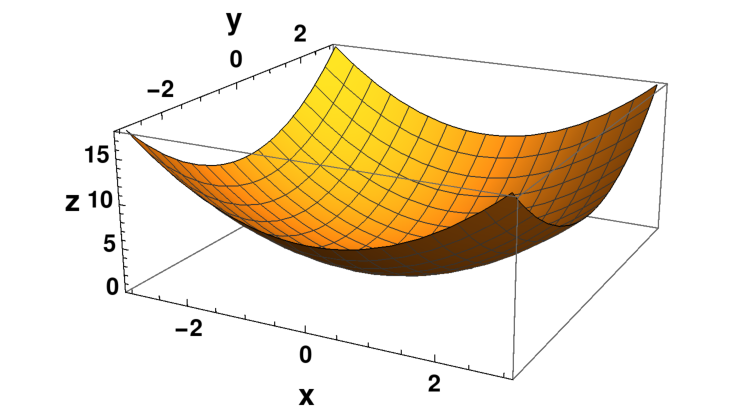
\includegraphics[width=0.46\textwidth]{Figuras/CampoEscalar.pdf}} \hspace{1cm}
        \subfigure[]{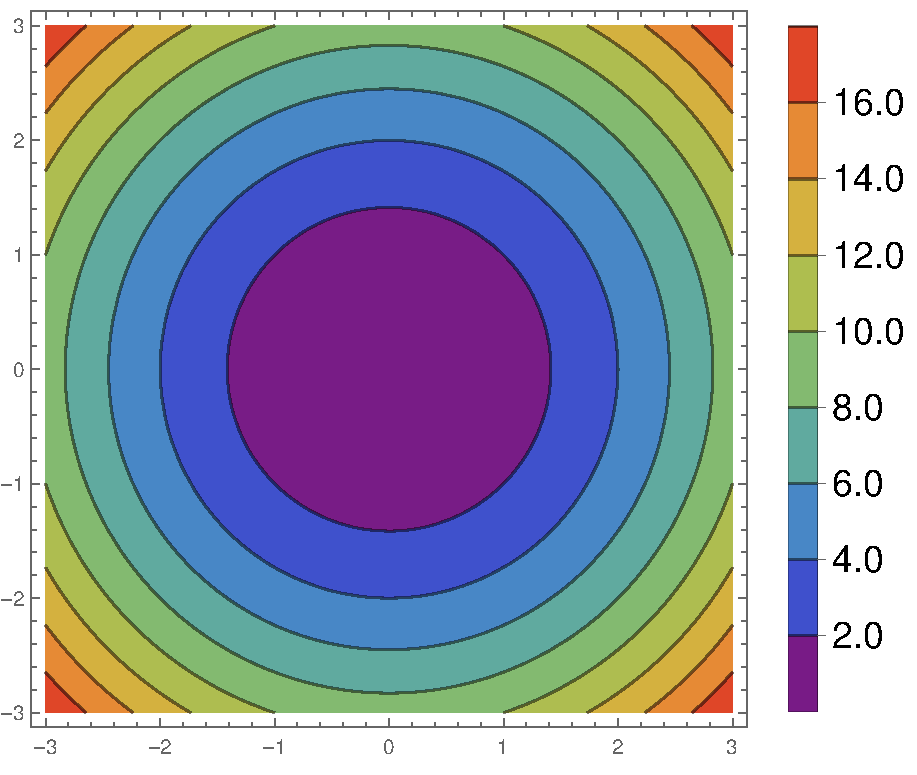
\includegraphics[width=0.35\textwidth]{Figuras/CurvasNivel.pdf}} 
        \caption{En (a), la gráfica del paraboloide $z = x^2+y^2$; y en (b), la gráfica de las curvas de nivel del paraboloide.}
        \label{fig:CampoEscalar}
    \end{figure}
\end{ejemplo}

Por otro lado, para campos escalares $\phi(x,y,z)$, no es posible tener una representación gráfica debido a que la gráfica de la función vive en un espacio de  cuatro dimensiones, pues, bajo la misma lógica del campo $\phi(x,y)$, un punto de la gráfica sería la $4$-tupla $(x,y,z,w) \in \mathbb{R}^4$, con $w = \phi(x,y,z)$. 

 
Un \textbf{campo vectorial} en el espacio de dos (o tres) dimensiones, es una función $\vec{V}$ que asigna a cada punto $(x,y)$ (o $(x,y,z)$) del espacio, un vector en dos (o tres) dimensiones dado por $\vec{V}(x,y)$ (o $\vec{V}(x,y,z)$).

Usando la base canónica de $\mathbb{R}^2$ y $\mathbb{R}^3$: $\{\hat{\imath},\hat{\jmath}\}$ y $\{\hat{\imath},\hat{\jmath}, \hat{k}\}$,  respectivamente. La notación para el campo vectorial $\vec{V}$ está dada por:
\begin{align*}
    \vec{V} (x,y) &= V_x(x,y) \hat{\imath} + V_y(x,y) \hat{\jmath}, \\
    \vec{V}(x,y,z) &= V_x(x,y,z) \hat{\imath} + V_y(x,y,z) \hat{\jmath} + V_z(x,y,z) \hat{k},   
\end{align*}

donde $V_x, V_y$ y $V_z$ son campos escalares.

Es habitual graficar las campos vectoriales dibujando en cada punto $(x,y)$ (o $(x,y,z)$) del espacio el vector $\Vec{V}(x,y)$ (o $\Vec{V}(x,y,z)$).

\begin{ejemplo}
\ 

    \begin{itemize}
        \item $\vec{V}(x,y) = -y \hat{\imath} + x \hat{\jmath}$.

        \begin{figure}[H]
            \centering
            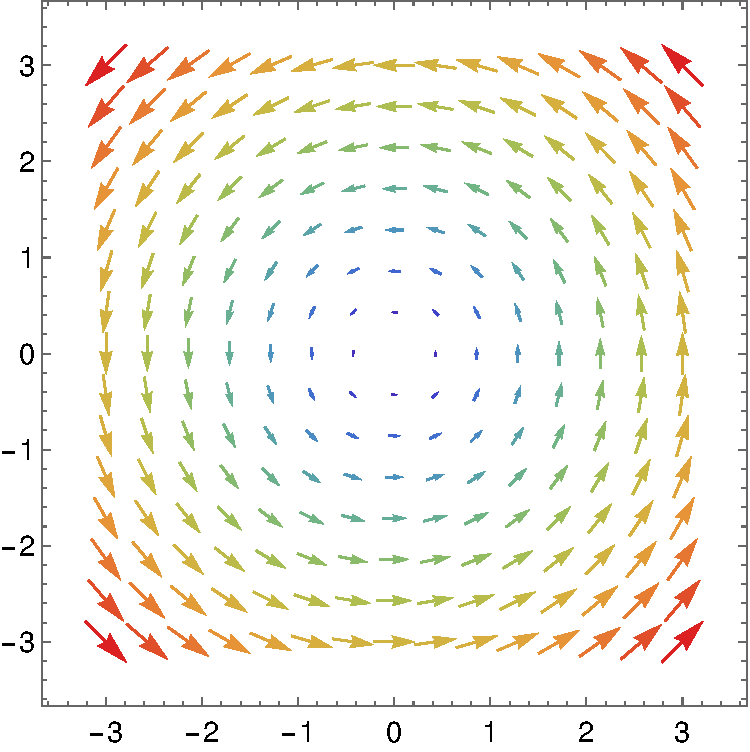
\includegraphics[scale = 0.45]{Figuras/CampoVectorial1.pdf}
            \caption{Gráfica del campo $\vec{V}(x,y) = -y \hat{\imath} + x \hat{\jmath}$.}
            \label{fig:Campo_Vectorial1}
        \end{figure}

        \item Campo en tres dimensiones con simetría radial: $\vec{V}(x,y,z) = x \hat{\imath} + y \hat{\jmath} + z \hat{k}$.

        \begin{figure}[H]
            \centering
            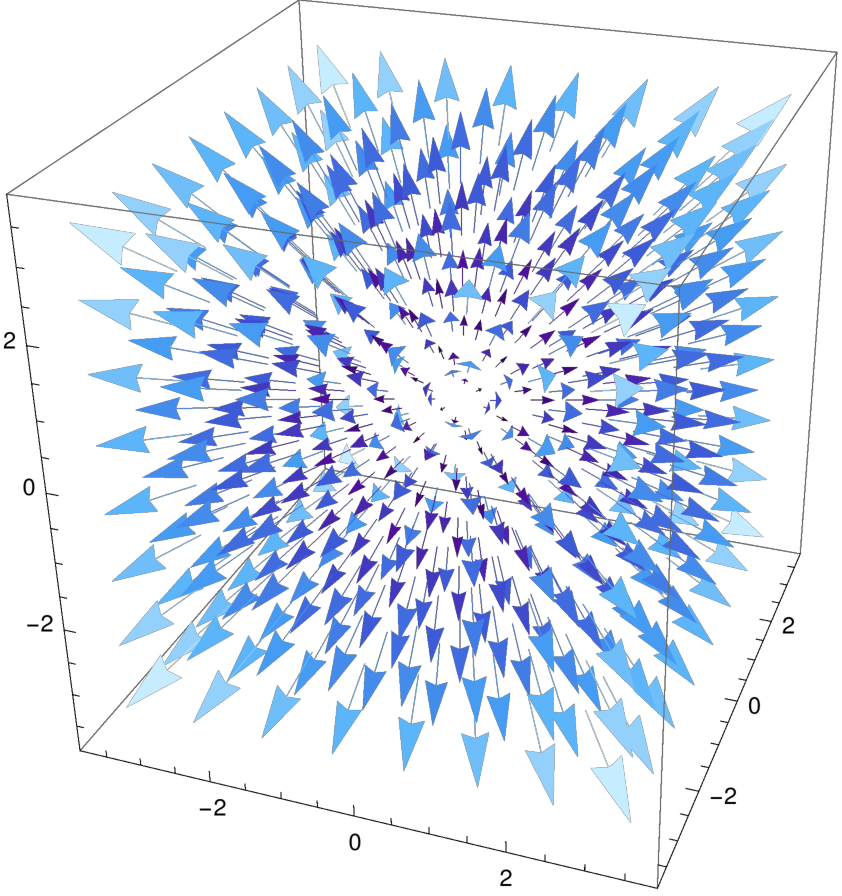
\includegraphics[scale = 0.44]{Figuras/CampoVectorial2.pdf}
            \caption{Gráfica del campo  $\vec{V}(x,y,z) = x \hat{\imath} + y \hat{\jmath} + z \hat{k}$.}
            \label{fig:Campo_Vectorial2}
        \end{figure}
    \end{itemize}
\end{ejemplo}

\section{Operadores vectoriales} \label{Operadores}

Sea la función de una variable real: $f(x)$. De los primeros cursos de Cálculo sabemos que si $f$ es derivable, la derivada $df/dx$ nos indica cómo cambia $f(x)$ con respecto $x$, geométricamente, corresponde a la pendiente de la gráfica $y = f(x)$. 

Si consideramos cantidades infinitesimales,
$$df = \left(\frac{df}{dx} \right) dx.$$

En palabras: Si incrementamos $x$ por una cantidad infinitesimal $dx$, entonces $f$ cambia por una cantidad $df$; la derivada es el factor de proporcionalidad.

\subsection*{Gradiente de un campo escalar}

Si consideramos ahora una función de tres variables: $f(x,y,z)$. Nos gustaría generalizar la noción de “derivada” de la función, que no depende de una sino de tres variables.

Una derivada debería decirnos cuán rápido una función cambia, para el caso de tres variables la situación es más complicada porque ya no tenemos solo una dirección en un eje para evaluar el cambio, sino varias direcciones (representadas como vectores en $\mathbb{R}^3$). 

Definimos, artesanalmente, la derivada parcial de $f(x,y,z)$ con respecto al eje $x_i$,
$$\frac{\partial f}{\partial x_i}, \quad \text{con} ~ x_i = x,y,z,$$

como la “variación” de $f$ con respecto a la dirección dada por el eje $x_i$, manteniendo el resto de las variables constantes. Por ejemplo, 
$$\frac{\partial}{\partial y}[2xy] = 2x,$$

donde hemos derivado suponiendo que $x$ es una constante.

Para saber cuánto varía $f$ cuando nos trasladamos un diferencial de posición $d\Vec{x} = dx \, \hat{\imath} + dy \,\hat{\jmath} + dz \,\hat{k}$, el Cálculo en varias variables nos entrega el siguiente teorema:
$$df = \left(\frac{\partial f}{\partial x}\right) dx + \left(\frac{\partial f}{\partial y}\right) dy +\left(\frac{\partial f}{\partial z}\right) dz.$$

Note que sólo nos bastó definir tres derivadas parciales para cuantificar el cambio infinitesimal de $f$, lo cual se justifica debido a que el espacio tridimensional $\mathbb{R}^3$ sólo tiene tres direcciones linealmente independientes.

Notemos que 
\begin{align*}
    df &= \left( \frac{\partial f}{\partial x} \hat{\imath} +  \frac{\partial f}{\partial y} \hat{\jmath} +  \frac{\partial f}{\partial z} \hat{k}\right)  \cdot (dx \, \hat{\imath} + dy \, \hat{\jmath} + dz \, \hat{k})\\
    &= (\Vec{\nabla} f) \cdot (d\Vec{x}),
\end{align*}

donde 
\begin{shaded}
$$\vec{\nabla}f(x,y,z) := \frac{\partial f}{\partial x} \hat{\imath} + \frac{\partial f}{\partial y} \hat{\jmath} +  \frac{\partial f}{\partial z} \hat{k}$$
\end{shaded}

es el \textbf{gradiente de $f$} (en coordenadas cartesianas).

\textbf{Nota:} Lo expuesto es cierto si $f(x,y,z)$ es un campo escalar diferenciable. \footnote{$f(x,y,z)$ se dice diferenciable si es posible aproximar la gráfica de la función en cada punto por un plano tangente a la gráfica. Además,  garantiza la existencia de las derivadas parciales.}

Si omitimos la función $f$, podemos definir el \textbf{operador nabla}:
\begin{shaded}
$$\vec{\nabla} :=  \hat{\imath} \frac{\partial}{\partial x} +  \hat{\jmath} \frac{\partial}{\partial y} +   \hat{k} \frac{\partial}{\partial z}.$$
\end{shaded}

El vector gradiente tiene dos \underline{interpretaciones geométricas} importantes:

\begin{enumerate}
\item En tres dimensiones, $\vec{\nabla}f(x,y,z)$ es un vector normal al plano tangente a la superficie $f ( x, y, z ) = C$ en cada punto. Para el caso de dos dimensiones, $\vec{\nabla}f(x,y)$ es un vector normal a la recta tangente a la curva $f(x,y) = C$.

\begin{figure}[H]
    \centering
    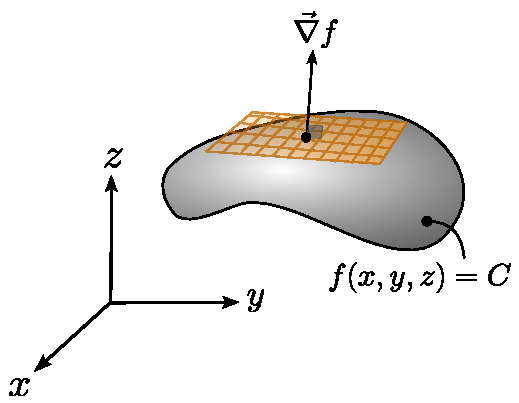
\includegraphics[scale = 0.8]{Figuras/Gradiente1.pdf}
    \caption{El gradiente como vector normal a la superficie $f(x,y,z) = C$.}
    \label{fig:Gradiente1}
\end{figure}

\item En dos dimensiones, $\vec{\nabla}f(x_0,y_0)$  indica la dirección del máximo incremento de $f(x,y)$ en el punto $(x_0,y_0)$. Para el caso de tres dimensiones, $\vec{\nabla}f(x_0,y_0,z_0)$  indica la dirección del máximo incremento de $f(x,y,z)$ en el punto $(x_0,y_0,z_0)$. 

\begin{figure}[H]
    \centering
    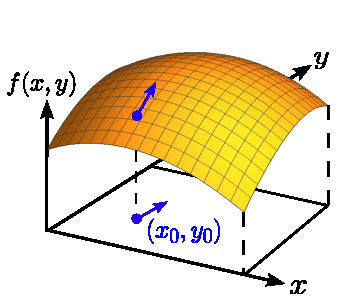
\includegraphics[scale = 0.89]{Figuras/Gradiente2.pdf}
    \caption{El gradiente como dirección de máximo incremento de $f(x,y)$ en $(x_0,y_0)$.}
    \label{fig:Gradiente2}
\end{figure}

\end{enumerate}

\begin{ejemplo}
    Determine el vector normal a la esfera $x^2+y^2+z^2 = 3$ en el punto $(1,1,1)$.

    \textbf{Solución:} Sea $f(x,y,z) = x^2+y^2+z^2$, 
    \begin{align*}
        \frac{\partial f}{\partial x} &= \frac{\partial}{\partial x}[x^2] + \cancelto{0}{\frac{\partial}{\partial x}[y^2]} + \cancelto{0}{\frac{\partial}{\partial x}[z^2]} = 2x,   \\
        \frac{\partial f}{\partial y} &=\cancelto{0}{\frac{\partial}{\partial y}[x^2]} + \frac{\partial}{\partial y}[y^2] + \cancelto{0}{\frac{\partial}{\partial y}[z^2]} = 2y, \\
        \frac{\partial f}{\partial z} &=\cancelto{0}{\frac{\partial}{\partial z}[x^2]} + \cancelto{0}{\frac{\partial}{\partial z}[y^2]} + \frac{\partial}{\partial z}[z^2]  = 2z.
    \end{align*}

    Luego, el gradiente de $f$ es
    $$\Vec{\nabla} f(x,y,z) = 2x \hat{\imath} + 2y \hat{\jmath} + 2z \hat{k}.$$

    Por lo tanto, el vector normal a la esfera en $(1,1,1)$ es $\Vec{\nabla} f(1,1,1) = 2 \hat{\imath} + 2 \hat{\jmath} + 2 \hat{k}.$
\end{ejemplo}

\subsection*{Divergencia de un campo vectorial}

Para un campo vectorial
$$\vec{V} (x,y,z) = V_x(x,y,z) \hat{\imath} + V_y(x,y,z) \hat{\jmath} + V_z(x,y,z) \hat{k} ,$$

la \textbf{divergencia} está definida por
\begin{shaded}
    $$\mbox{div} ~\vec{V} \equiv \vec{\nabla} \cdot \vec{V} := \frac{\partial V_x}{\partial x} + \frac{\partial V_y}{\partial y} + \frac{\partial V_z}{\partial z}.$$
\end{shaded}

\textbf{Nota:} Cualquier campo vectorial para el cual $\vec{\nabla} \cdot \vec{V} = 0$ se dice que es \textit{solenoidal}.

Diremos que la divergencia puede ser considerada como una medida cuantitativa de cuanto un campo vectorial “diverge” o “converge” en un punto dado. 

\begin{figure}[H]
    \centering
    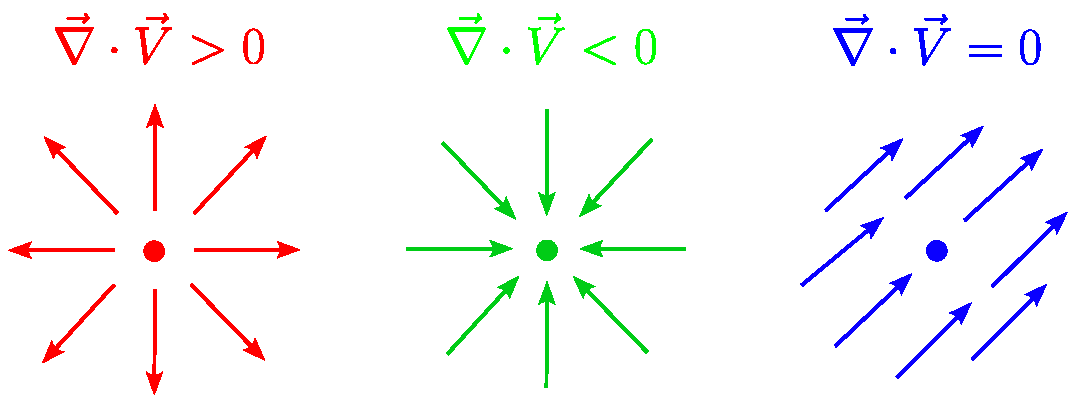
\includegraphics[scale = 0.55]{Figuras/Divergencia.pdf}
    \caption{Interpretación física de la divergencia.}
    \label{fig:sign_divergence}
\end{figure}

Analicemos los tres posibles casos:

\begin{enumerate}
\item Si $\vec{\nabla} \cdot \vec{V} >0$ en algún punto, estamos en presencia de una \textit{fuente} o \textit{manantial} desde donde el campo vectorial radia hacia el exterior. 

\item Si $\vec{\nabla} \cdot \vec{V} < 0$ estamos en presencia de un \textit{sumidero} pues el campo “converge” hacia dicho  punto.

\item  Si $\vec{\nabla} \cdot \vec{V} =0$ el campo no converge ni diverge (no hay fuentes ni sumideros); no pueden tener extremos localizados, las líneas solo pueden ser cerradas, o ir del infinito o al infinito, o dar vueltas sobre sí mismas, sin llegar a cerrarse.
\end{enumerate}

\begin{ejemplo}
    En mecánica de fluidos, la distribución de las velocidades del fluido es descrita por un campo vectorial $v(x, y, z, t)$. Esto representa la velocidad del fluido en el punto $(x, y, z)$ en el instante $t$. En nuestro caso omitiremos la dependencia temporal. Suponga que el campo de velocidades de un fluido es
    $$\Vec{v}(x,y) = (x^2-y^2) \hat{\imath} + 2xy \hat{j}$$

    \begin{figure}[H]
    \centering
    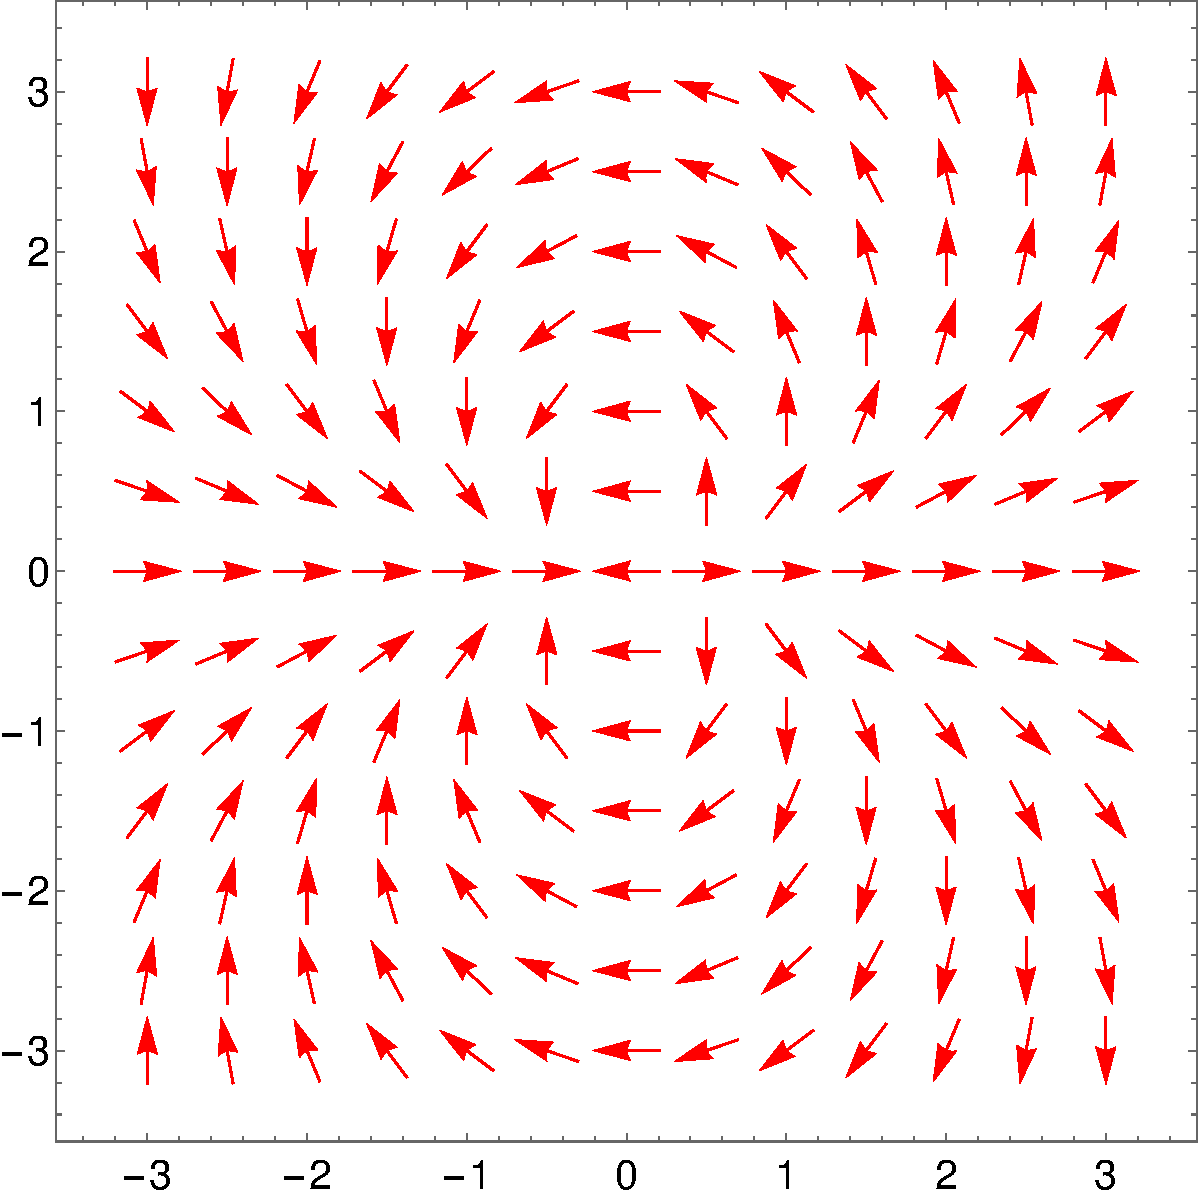
\includegraphics[scale = 0.3]{Figuras/Ej-Divergencia}
    \caption{Gráfica del campo de velocidades $\Vec{v}(x,y) = (x^2-y^2) \hat{\imath} + 2xy \hat{j}$ normalizado.}
    \label{fig:Ej_Divergencia}
    \end{figure}

    Calcule la divergencia y determine si en el punto $(1,2)$ es más una fuente o sumidero.

    \textbf{Solución:} La divergencia está dada por
    $$\vec{\nabla} \cdot \Vec{v} = \frac{\partial}{\partial x}[x^2-y^2] + \frac{\partial}{\partial y}[2xy] = 2x+2x = 4x. $$

    En el punto $(1,2)$, $\vec{\nabla} \cdot \Vec{v}(1,2) = 4 > 0$. Por lo tanto, en este punto se tiene más una fuente que un sumidero. Físicamente, la densidad del fluido decrece en ese punto.
\end{ejemplo}
  

\subsection*{Rotacional de un campo vectorial}

Sea el campo vectorial
$$\vec{V} (x,y,z) = V_x(x,y,z) \hat{\imath} + V_y(x,y,z) \hat{\jmath} + V_z(x,y,z) \hat{k}.$$

El \textbf{rotor} (o \textbf{rotacional}) de $\vec{V}$ está definido por 
\begin{shaded}
 $$\mbox{rot} ~ \vec{V} := \left( \frac{\partial V_z}{\partial y} - \frac{\partial V_y}{\partial z} \right) \hat{\imath} + \left( \frac{\partial V_x}{\partial z} - \frac{\partial V_z}{\partial x} \right) \hat{\jmath} + \left( \frac{\partial V_y}{\partial x} - \frac{\partial V_x}{\partial y} \right) \hat{k}.$$   
\end{shaded}

Otra forma de expresar el rotacional de un campo vectorial es
\begin{shaded}
$$\mbox{rot} ~ \vec{V} \equiv \vec{\nabla} \times \vec{V} = \left| \begin{array}{ccc}
\hat{\imath} & \hat{\jmath} & \hat{k}  \\
\frac{\partial}{\partial x} & \frac{\partial}{\partial y} & \frac{\partial}{\partial z}  \\
V_x & V_y & V_z
\end{array} \right|.$$  
\end{shaded}

El rotor asociado a un campo vectorial $\vec{V}$ es otro campo vectorial, y por tanto el rotor calculado en un punto es un vector. El \textit{rotor} es un operador vectorial $(\vec{\nabla} \times)$ que muestra la tendencia de un campo vectorial a inducir una rotación alrededor de un punto.

Si el rotor de un campo vectorial es cero en un punto significa que el campo vectorial no tiene rotaciones en ese punto (\textit{campo irrotacional}). En cambio si el rotor es distinto de cero significa que el campo tiene circulación o remolinos. En la siguiente figura se ilustra los dos casos para un campo vectorial $\Vec{V}$.

\begin{figure}[H]
    \centering
    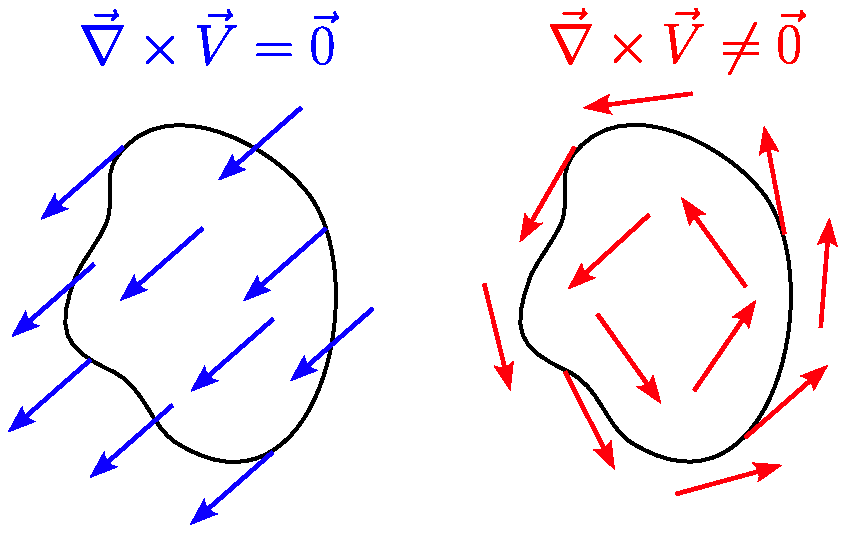
\includegraphics[scale = 0.52]{Figuras/Rotor.pdf}
    \caption{Interpretación física del rotacional.}
    \label{fig:rotor}
\end{figure}

\begin{ejemplo}
    Consideremos el campo vectorial
    $$\Vec{F}(x,y,z) = y \hat{\imath} - x\hat{\jmath}.$$
    
    El rotor está dado por
    
    $$\vec{\nabla} \times \vec{F} = \left| \begin{array}{ccc}
    \hat{\imath} & \hat{\jmath} & \hat{k}  \\
    \frac{\partial}{\partial x} & \frac{\partial}{\partial y} & \frac{\partial}{\partial z}  \\
    y & -x & 0
    \end{array} \right| = 0 \hat{\imath} + 0 \hat{\jmath} + \left( \frac{\partial}{\partial x}[-x] - \frac{\partial}{\partial y} [y]\right) \hat{k} = -2 \hat{k}.$$ 

    \begin{figure}[H]
        \centering
        \subfigure[]{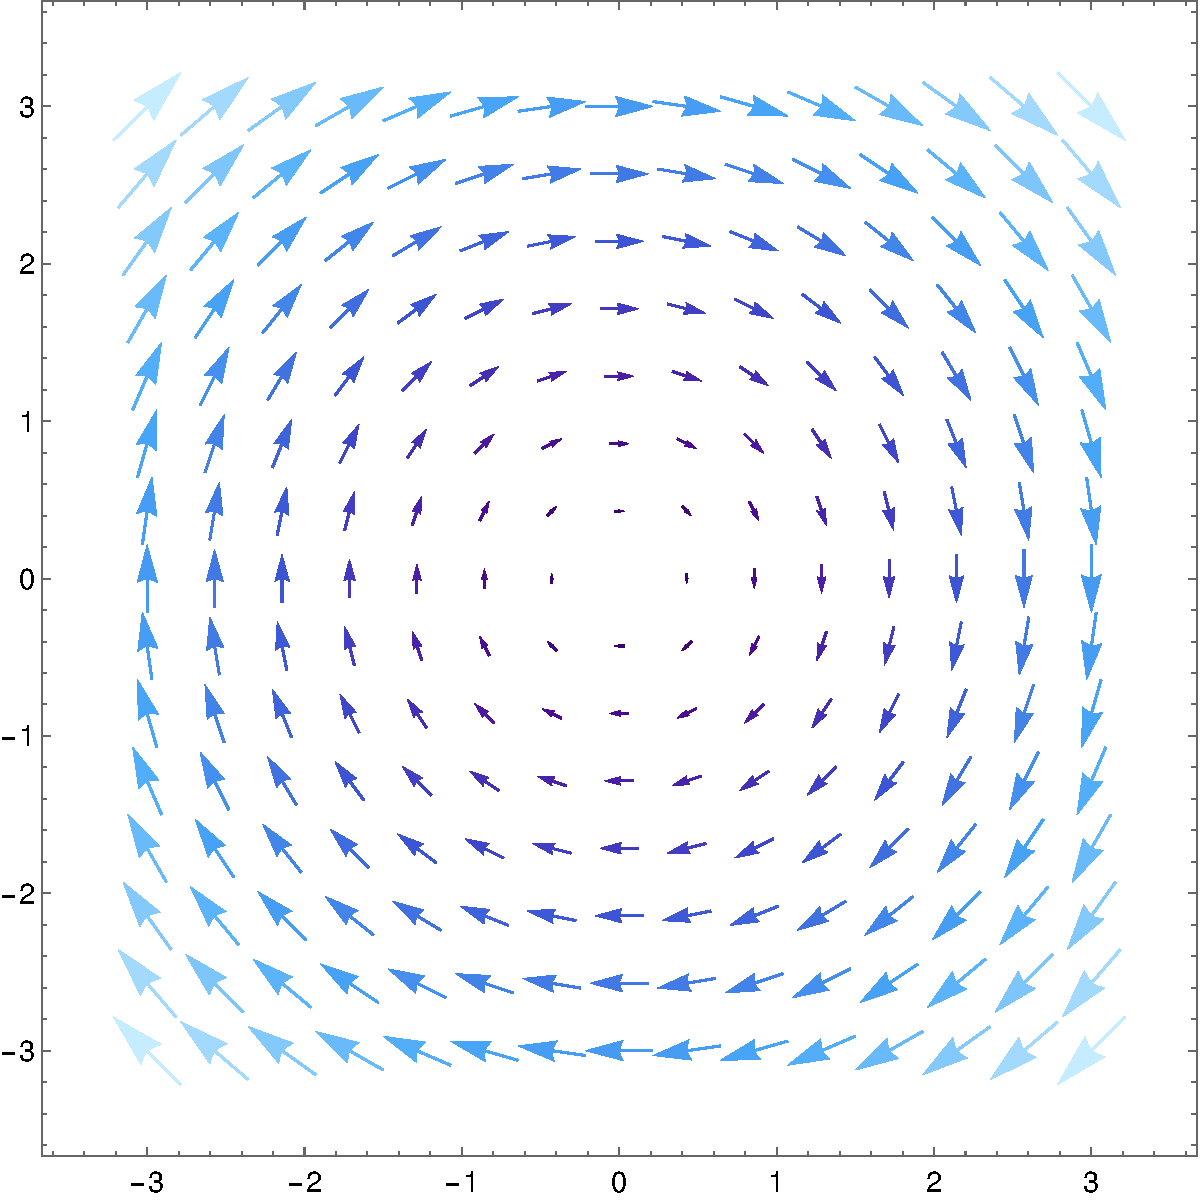
\includegraphics[width=0.36\textwidth]{Figuras/Ej-Rotor-1.pdf}} \hspace{1cm}
        \subfigure[]{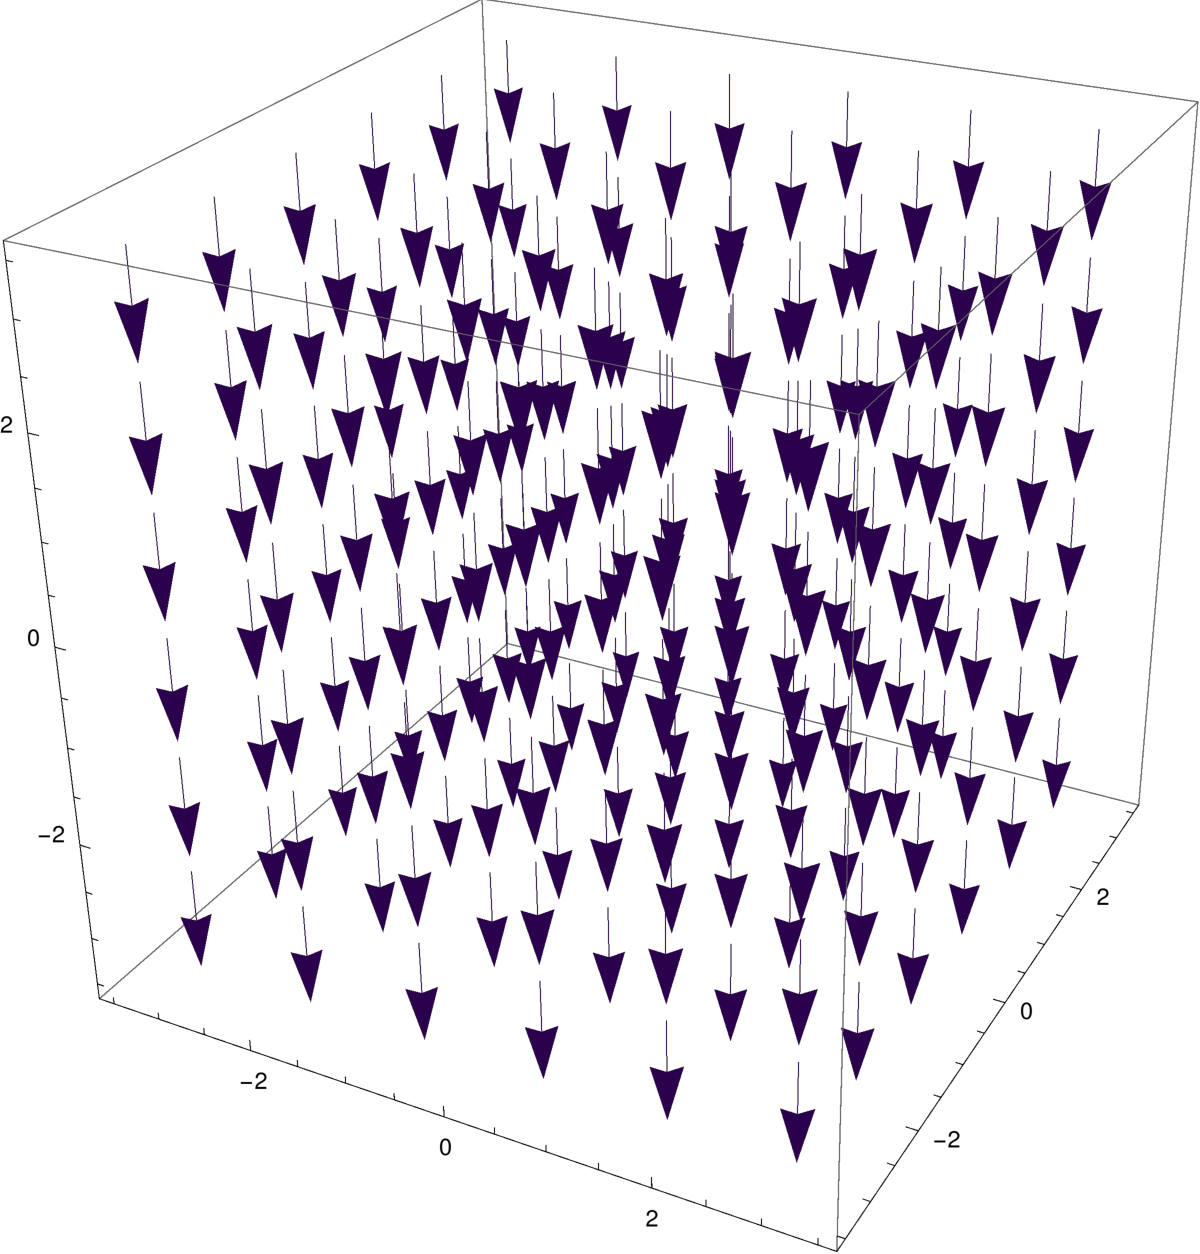
\includegraphics[width=0.36\textwidth]{Figuras/Ej-Rotor-2.pdf}} 
        \caption{Gráfica del campo vectorial $\Vec{F}(x,y,z) = y \hat{\imath} - x\hat{\jmath}$ (a) y su rotacional (b).}
        \label{fig:Ej_Rotor}
    \end{figure}
    
    El campo vectorial resultante describe que la circulación en todos los puntos será en torno de la dirección del eje $z$ negativo. Además, al ser un campo vectorial uniforme, el objeto descrito antes tendrá la misma intensidad del rotacional independiente de donde se sitúe.
\end{ejemplo}

\subsection*{Laplaciano}

En muchas aplicaciones Físicas aparecen ciertas combinaciones del gradiente, la divergencia y el rotacional. Una de ellas es la divergencia de un gradiente.

Sea $f(x,y,z)$ un campo escalar diferenciable:
\begin{align*}
    \vec{\nabla} \cdot \vec{\nabla} f &=  \left( \hat{\imath} \frac{\partial}{\partial x}  + \hat{\jmath} \frac{\partial}{\partial y}   + \hat{k}\frac{\partial}{\partial z}  \right) \cdot \left( \frac{\partial f}{\partial x} \hat{\imath} + \frac{\partial f}{\partial y} \hat{\jmath} + \frac{\partial f}{\partial z} \hat{k} \right) \\
&= \frac{\partial^2 f }{\partial x^2} + \frac{\partial^2 f}{\partial y^2} + \frac{\partial^2 f}{\partial z} .  
\end{align*}

De aquí definimos el \textbf{Laplaciano} de $f$ como
\begin{shaded}
    $$\nabla^2 f := \frac{\partial^2 f }{\partial x^2} + \frac{\partial^2 f}{\partial y^2} + \frac{\partial^2 f}{\partial z^2}.$$
\end{shaded}

\subsection*{Propiedades de los operadores vectoriales}

\begin{teorema} \label{Prop-Op-Vect}
Sean $\Vec{A}$ y $\Vec{B}$ dos campos vectoriales diferenciables y, $\phi$ y $\psi$ dos campos escalares diferenciables de $(x,y,z)$. Entonces,
\begin{enumerate}
    \item $\Vec{\nabla}(\phi + \psi) = \Vec{\nabla} \phi + \Vec{\nabla} \psi$.

    \item $\Vec{\nabla} \cdot (\vec{A} + \Vec{B}) = \Vec{\nabla} \cdot \Vec{A} + \Vec{\nabla} \cdot \Vec{B}$.

    \item $\Vec{\nabla} \times (\vec{A} + \Vec{B} ) = \Vec{\nabla} \times \Vec{A} + \Vec{\nabla} \times \Vec{B}$.

    \item $\Vec{\nabla} \cdot (\phi \Vec{A}) = (\Vec{\nabla} \phi) \cdot \Vec{A} + \phi (\Vec{\nabla} \cdot \Vec{A})$.

    \item $\Vec{\nabla} \times (\phi \Vec{A}) = (\Vec{\nabla} \phi) \times \Vec{A} + \phi(\Vec{\nabla} \times \Vec{A})$.

    \item $\Vec{\nabla} \cdot (\Vec{A} \times \Vec{B}) = \Vec{B} \cdot (\Vec{\nabla} \times \Vec{A}) - \Vec{A} \cdot (\Vec{\nabla} \times \Vec{B})$.

    \item $\Vec{\nabla} \times (\Vec{A} \times \Vec{B}) = (\Vec{B} \cdot \Vec{\nabla}) \Vec{A} - (\Vec{A} \cdot  \Vec{\nabla}) \Vec{B} + \Vec{A}( \Vec{\nabla} \cdot \Vec{B}) - \Vec{B}( \Vec{\nabla} \cdot \Vec{A})$.

    \item $ \Vec{\nabla}(\Vec{A} \cdot \Vec{B}) = (\Vec{B}  \cdot \Vec{\nabla}) \Vec{A} + (\Vec{A} \cdot  \Vec{\nabla}) \Vec{B} + \Vec{A} \times ( \Vec{\nabla} \times \Vec{B}) + \Vec{B} \times ( \Vec{\nabla} \times \Vec{A})$.

    \item Si $\phi$ es de clase $C^2$, $\vec{\nabla} \times  \Vec{\nabla} \phi = \Vec{0}$.

    \item Si $\Vec{A}$ es de clase $C^2$, $\vec{\nabla} \cdot  (\Vec{\nabla} \times \Vec{A}) = 0$.

    \item $\Vec{\nabla} \times (\Vec{\nabla} \times \Vec{A}) = \Vec{\nabla} (\Vec{\nabla} \cdot \Vec{A}) - (\Vec{\nabla} \cdot \Vec{\nabla}) \Vec{A} = \Vec{\nabla}(\Vec{\nabla} \cdot \Vec{A}) - \Vec{\nabla}^2 \Vec{A}$.
\end{enumerate}
\end{teorema}

\begin{demo}
Ejercicio para el lector.
\end{demo}

\textbf{Observación:} El orden de como se aplica el operador es importante. Por ejemplo,
\begin{align*}
    (\Vec{B} \cdot \Vec{\nabla}) \Vec{A} &= \left( B_x \frac{\partial}{\partial x} + B_y \frac{\partial}{\partial y} + B_z \frac{\partial}{\partial z}\right) \left( A_x \hat{\imath} + A_y \hat{\jmath} + A_z \hat{k}\right) \\
    &= \left(B_x \frac{\partial A_x}{\partial x} + B_y \frac{\partial A_x}{\partial y}  + B_z\frac{\partial A_x}{\partial z} \right) \hat{\imath} + \left(B_x \frac{\partial A_y}{\partial x} + B_y \frac{\partial A_y}{\partial y}  + B_z\frac{\partial A_y}{\partial z} \right) \hat{\jmath} \\
    & + \left(B_x \frac{\partial A_z}{\partial x} + B_y \frac{\partial A_z}{\partial y}  + B_z\frac{\partial A_z}{\partial z} \right) \hat{k}
\end{align*}

es distinto de
\begin{align*}
    \Vec{B} ( \Vec{\nabla} \cdot \Vec{A}) &= \left( B_x \hat{\imath} + B_y \hat{\jmath} + B_z \hat{k}\right) \left( \frac{\partial A_x}{\partial x} + \frac{\partial A_y}{\partial y} + \frac{\partial A_z}{\partial z}\right)  \\
    &= \left(B_x \frac{\partial A_x}{\partial x} + B_x \frac{\partial A_y}{\partial y}  + B_x\frac{\partial A_z}{\partial z} \right) \hat{\imath} + \left(B_y \frac{\partial A_x}{\partial x} + B_y \frac{\partial A_y}{\partial y}  + B_y \frac{\partial A_z}{\partial z} \right) \hat{\jmath} \\
    & + \left(B_z \frac{\partial A_x}{\partial x} + B_z \frac{\partial A_y}{\partial y}  + B_z\frac{\partial A_z}{\partial z} \right) \hat{k}.
\end{align*}

\section{Integrales vectoriales}

A lo largo del curso nos encontraremos con campos escalares y vectoriales que varían en el espacio, y necesitaremos con frecuencia integrar estos campos a lo largo de líneas, sobre superficies y a través de volúmenes.

\subsection{Integrales de línea}

Las integrales de línea pueden tener las siguients formas:
\begin{equation*}
\int_C \phi \, d\vec{x}, \quad \int_C \vec{F} \cdot d\vec{x}, \quad \int_C \vec{F} \times d\vec{x},
\end{equation*}

donde $\phi$ es un campo escalar, $\vec{F}$ un campo vectorial y $d\vec{x}$ un vector de desplazamiento infinitesimal. Si $C$ es una curva cerrada, se escribe: 
$$\oint \vec{F} \cdot d\vec{x}.$$

Las integrales $\int_C \vec{F} \cdot d\vec{x}$ son las más usuales en electromagnetismo y es común escribir
$$\int_A^B \Vec{F} \cdot d\vec{x},$$

donde $A$ y $B$ son los puntos iniciales y finales de la trayectoria o curva $C$.

\textbf{Nota:} El sentido de recorrido de la curva cambia el signo del valor de la integral, ésto es,
$$\int_A^B \Vec{F} \cdot d\Vec{x} = - \int_B^A \Vec{F} \cdot d\Vec{x}. $$

\begin{ejemplo}
    Calcule la integral de línea del campo vectorial $\Vec{F}(x,y,z) = y^2 \hat{\imath} + 2x(y+1) \hat{\jmath}$ desde el punto $A = (1,1,0)$ hasta el punto $B = (2,2,0)$, siguiendo las trayectorias (1) y (2) en la figura \ref{fig:Ej_Int_Linea}.

    \begin{figure}[H]
        \centering
        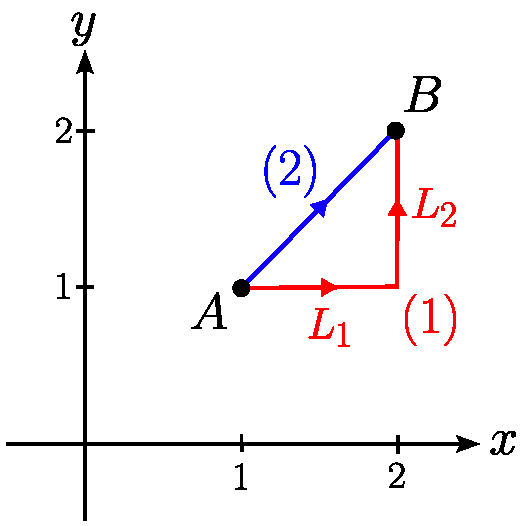
\includegraphics[scale = 0.55]{Figuras/Ej-Integral-Linea.pdf}
        \caption{Curva de integración.}
        \label{fig:Ej_Int_Linea}
    \end{figure}

    \textbf{Solución:} La trayectoria (1) se divide en dos partes. A lo largo del segmento horizontal $L_1$, no hay cambios en $y$ ni en $z$, entonces $dy = dz = 0$ y $d\Vec{x} = dx \hat{\imath}$. Además, a lo largo del segmento, $1 \leq x \leq 2$ e $y = 1$.

    Así,
    $$\int_{L_1} \Vec{F} \cdot d \Vec{x} = \int_1^2 ((1)^2 \hat{\imath} + 2x(1+1) \hat{\jmath}) \cdot (dx \hat{\imath}) = \int_1^2 dx = 1.$$

    En el segmento vertical $L_2$, no hay cambios en $x$ ni en $z$, entonces $dx = dz = 0$ y $d\Vec{x} = dy \hat{\jmath}$. Además, a lo largo de este segmento, $x = 2$ y $1 \leq y \leq 2$.

    Así,
    $$\int_{L_2} \Vec{F} \cdot d \Vec{x} = \int_1^2 (y^2 \hat{\imath} + 2(2)(y+1) \hat{\jmath}) \cdot (dy \hat{\jmath}) = \int_1^24(y+1) dy = 10.$$

    Por lo tanto, la integral de línea en torno a la trayectoria (1) es
    $$\int_A^B \Vec{F} \cdot d\Vec{x} = \int_{L_1} \Vec{F} \cdot d \Vec{x} + \int_{L_2} \Vec{F} \cdot d \Vec{x} = 11.$$

    Por otro lado, para la trayectoria (2), no hay cambios en $z$, así que $dz = 0$. Pero, $y = x$ y, en consecuencia,
    $$dx = dy \Rightarrow d\Vec{x} = dx \hat{\imath} + dy \hat{\jmath} = dx \hat{\imath} + dx \hat{\jmath} = (\hat{\imath} + \hat{\jmath} ) dx.$$

    Hemos elegido la variable $x$ para integrar, lo cual es arbitrario (se llega al mismo resultado eligiendo $y$). Entonces,
    $$\int_A^B \Vec{F} \cdot d\Vec{x} = \int_1^2 (x^2 \hat{\imath} + 2x(x+1) \hat{\jmath}) \cdot (\hat{\imath} + \hat{\jmath} ) dx = \int_1^2 3x^2 + 2x \,dx = 10.$$
\end{ejemplo}

\textbf{Observaciones:}

\begin{enumerate}
    \item Las curvas del ejemplo estaban constituidas de segmentos y el campo vectorial estaba escrito en coordenadas $(x,y,z)$, lo cual facilitó el cálculo usando coordenadas cartesianas. Sin embargo, si se hubiese integrado, por ejemplo, sobre un arco de circunferencia, las coordenadas cartesianas dejan de ser útiles. Entonces, dependiendo de la curva y la forma del campo vectorial, se elige el sistema de coordenadas apropiado para atacar la integral.

    \item En general, las integrales de línea dependen de la trayectoria que unen los puntos.
\end{enumerate}


Un tipo de campo vectorial muy importante al momento de calcular integrales de línea son los campo \textbf{conservativos}. 

Un campo vectorial $\vec{F}$ se dice \textbf{conservativo} si existe un campo escalar $\phi$ tal que
\begin{equation*}
\vec{F} = \vec{\nabla} \phi.
\end{equation*}

De aquí se deriva el \textbf{teorema fundamental para gradientes}, el cual expresa que
\begin{shaded}
   \begin{equation*}
\int_A^B \vec{F} \cdot d\vec{r} = \int_A^B \Vec{\nabla} \phi \cdot d\Vec{x} = \phi(B) - \phi(A),
\end{equation*} 
\end{shaded}

para cualquier curva que una $A$ y $B$.

Si $\Vec{F}$ es un campo conservativo, se verifica:
\begin{enumerate}
\item $\int \vec{F} \cdot d\vec{r}$ es independiente de la trayectoria tomada.

\item $\oint\vec{F} \cdot d\vec{r} = 0$ para toda trayectoria cerrada.

\item $\vec{\nabla} \times \vec{F} = \vec{0}$, es decir, un campo conservativo es irrotacional.
\end{enumerate}

\subsection{Integrales de superficie}

Las integrales de superficie pueden tener las siguientes formas>
\begin{equation*}
\iint_S \phi d\vec{S}, \quad \iint_S \vec{F} \cdot d\vec{S}, \quad \iint_S \vec{F} \times d\vec{S},
\end{equation*}

donde $\phi$ es un campo escalar, $\vec{F}$ un campo vectorial y $d\vec{S}$ un vector de superficie infinitesimal de la superficie $S$ la cual puede ser abierta o cerrada. De nuevo, para superficies cerradas se usa el símbolo $\oiint$.

El elemento $d\vec{S}$ se define perpendicular a la superficie y a veces se escribe como $d\vec{S} = \hat{n} dS$, donde $\hat{n}$ es un vector unitario perpendicular a la superficie en la posición del elemento y $dS$ es la magnitud (escalar) de $d\vec{S}$. Si la superficie encierra un volumen, $\hat{n}$ apunta fuera del volumen (a menos que se indique lo contrario), ver figura \ref{fig:Superficies}-(a).

Para el caso de una superficie $S$ que no está en un volumen cerrado, diremos que la orientación de la curva cerrada $C$, trazada sobre el contorno de $S$, es compatible con la orientación de $S$ si la orientación de $C$ y $S$ cumplen con la regla de la mano derecha, ver figura \ref{fig:Superficies}-(b).

\begin{figure}[H]
    \centering
    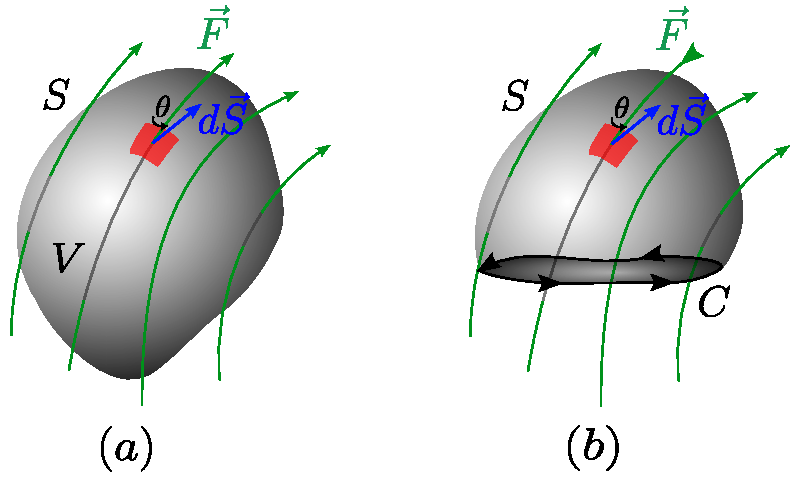
\includegraphics[scale = 0.8]{Figuras/ElementoSuperficie.pdf}
    \caption{En $(a)$ una superficie cerrada y en $(b)$ una superficie abierta. En cada caso se muestra un vector normal a la superficie $d\Vec{S}$, el cual forma un ánuglo $\theta$ con el campo vectorial $\Vec{F}$.}
    \label{fig:Superficies}
\end{figure}


Las integrales de superficie más comunes son las de tipo 
\begin{equation*}
\Phi_F = \iint_S \vec{F} \cdot d\vec{S},
\end{equation*}

llamadas integrales de \textbf{flujo}.

\begin{ejemplo}
    Calcule la integral de superficie de 
    $$\Vec{F}(x,y,z) = 2xz \hat{\imath} + (x+2) \hat{\jmath} + y(z^2-3) \hat{k}$$

    sobre las cinco caras (no incluyendo la basal) de la caja cúbica en la figura \ref{fig:Ej_Int_Superficie}.

    \begin{figure}[H]
        \centering
        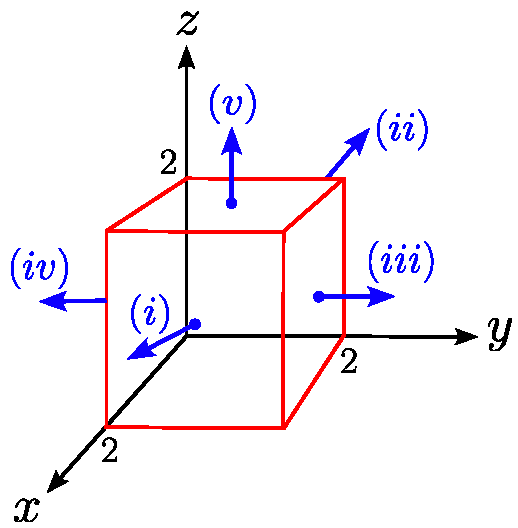
\includegraphics[scale = 0.7]{Figuras/Ej-Integral-Superficie.pdf}
        \caption{Superficie de integración.}
        \label{fig:Ej_Int_Superficie}
    \end{figure}

    \textbf{Solución:}  Tomando las caras una a la vez.

    \begin{itemize}
        \item[(i)] Para la cara $x = 2$, $d\Vec{S} = dydz \hat{\imath}$ con $0 \leq y \leq 2$ y $0 \leq z \leq 2$. Entonces,
        \begin{align*}
             \iint \Vec{F} \cdot d\Vec{S} &= \int_0^2 \int_0^2 (4z \hat{\imath} + (2+2) \hat{\jmath} + y(z^2-3) \hat{k}) \cdot (dydz \hat{\imath})  \\
             &= \int_0^2 \left( \int_0^2 4z dy\right) dz\\
             &= 4 \int_0^2 z \left( \int_0^2 dy \right) dz \\
             &= 4 \int_0^2 2z \,dz \\
             &= 16.
        \end{align*}

        \item[(ii)] Para la cara $x = 0$, $d\Vec{S} = -dydz \hat{\imath}$ con $0 \leq y \leq 2$ y $0 \leq z \leq 2$. Entonces,
        \begin{align*}
             \iint \Vec{F} \cdot d\Vec{S} &= \int_0^2 \int_0^2 (0\hat{\imath} + (0+2) \hat{\jmath} + y(z^2-3) \hat{k}) \cdot (-dydz \hat{\imath})  \\
             &= \int_0^2 \left( \int_0^2 0 \, dy\right) dz\\
             &= 0.
        \end{align*}

        \item[(iii)] Para la cara $y = 2$, $d\Vec{S} = dxdz \hat{\jmath}$ con $0 \leq x \leq 2$ y $0 \leq z \leq 2$. Entonces,
        \begin{align*}
             \iint \Vec{F} \cdot d\Vec{S} &= \int_0^2 \int_0^2 (2xz \hat{\imath} + (x+2) \hat{\jmath} + 2(z^2-3) \hat{k}) \cdot (dxdz \hat{\jmath})  \\
             &= \int_0^2 \left( \int_0^2 x+2 \,dx\right) dz\\
             &=  \int_0^2   6 \, dz \\
             &= 12.
        \end{align*}

        \item[(iv)] Para la cara $y = 0$, $d\Vec{S} = -dxdz \hat{\jmath}$ con $0 \leq x \leq 2$ y $0 \leq z \leq 2$. Entonces,
        \begin{align*}
             \iint \Vec{F} \cdot d\Vec{S} &= \int_0^2 \int_0^2 (2xz \hat{\imath} + (x+2) \hat{\jmath} + 0 \hat{k}) \cdot (-dxdz \hat{\jmath})  \\
             &=- \int_0^2 \left( \int_0^2 x+2 \, dx\right) dz\\
             &=  - 12.
        \end{align*}

        \item[(v)] Para la cara $z = 2$, $d\Vec{S} = dxdy \hat{k}$ con $0 \leq x \leq 2$ y $0 \leq y \leq 2$. Entonces,
        \begin{align*}
             \iint \Vec{F} \cdot d\Vec{S} &= \int_0^2 \int_0^2 (4x \hat{\imath} + (x+2) \hat{\jmath} + y((2)^2-3) \hat{k}) \cdot (dxdy \hat{k})  \\
             &= \int_0^2 \left( \int_0^2 y\, dx\right) dy\\
             &= \int_0^2 2y\,dy \\
             &= 4.
        \end{align*}
    \end{itemize}

    Por lo tanto, el flujo total es
    $$\iint_S \Vec{F} \cdot d\Vec{S} = 16 + 0 + 12 - 12 + 4 = 20.$$
\end{ejemplo}

\textbf{Observación:} Al igual que para las integrales de líneas, la forma del campo vectorial y de la superficie permitió que la integral sea sencillamente calculada en coordenadas cartesianas, pero si nos enfrentamos a, por ejemplo, un cilindro, es conveniente utilizar otras coordenadas.

\subsection{Integral de volumen}

Una integral de volumen es una expresión de la forma
$$\iiint_V f(x,y,z) \,dV,$$

donde $f(x,y,z)$ es un campo escalar y $dV$ un elemento infinitesimal de volumen. En coordenadas cartesianas,
$$dV = dx dy dz.$$

Ocasionalmente nos encontraremos con integrales de volumen de campos vectoriales:
\begin{align*}
  \iiint_V \vec{F} dV &= \iiint_V (F_x \hat{\imath} + F_y \hat{\jmath} + F_z \hat{k}) \,dV\\
  &=\hat{\imath} \iiint_V F_x dV +  \hat{\jmath} \iiint_V F_y dV  + \hat{k} \iiint_V F_z dV, 
\end{align*}

porque los vectores unitarios ($\hat{\imath}$, $\hat{\jmath}$ y $\hat{k}$) son constantes, salen de la integral.

\begin{ejemplo}
    Calcule la integral de volumen del campo escalar $f(x,y,z) = x^2$ sobre el tetraedro con vértices $(0,0,0)$, $(1,0,0)$, $(0,1,0)$ y $(0,0,1)$.

    \textbf{Solución:} La gráfica del tetraedro en conjunto con su proyección en el plano $xy$ se ilustra en la figura \ref{fig:Ej-Int_Volumen}.

    \begin{figure}[H]
        \centering
        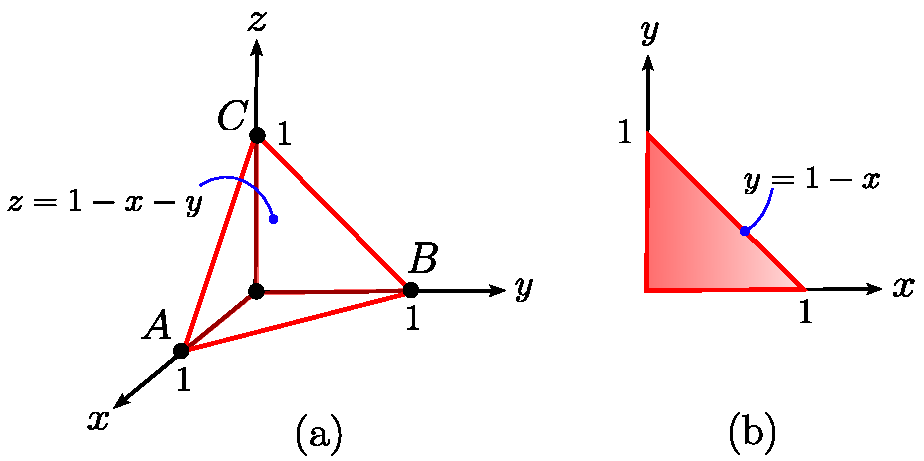
\includegraphics[scale = 0.7]{Figuras/Ej-Integral-Volumen.pdf}
        \caption{En (a) el tetraedro y en (b) la proyección (sombra) del tetraedro en el plano $xy$.}
        \label{fig:Ej-Int_Volumen}
    \end{figure}

    Determinemos la ecuación del plano que pasa por $A = (1,0,0)$, $B = (0,1,0)$ y $C = (0,0,1)$. Sean los vectores
    \begin{align*}
        \overrightarrow{CA} &= (1,0,0) - (0,0,1) = (1,0,-1), \\
        \overrightarrow{CB} &= (0,1,0) - (0,0,1) = (0,1,-1).
    \end{align*}

    Un vector normal al plano es
    $$\Vec{n} = \overrightarrow{CA} \times  \overrightarrow{CB} = (1,1,1).$$

    Entonces, la ecuación del plano está dada por
    $$\Vec{n} \cdot ( (x,y,z) - (1,0,0)) = 0 \Rightarrow x + y + z = 1.$$
    
    Para calcular este tipo de integrales debemos primero elegir un orden de integración, en nuestro caso será integrar en la variable $z$, luego en la variable $y$ y por último en la variable $x$, ésto es, el orden $dzdydx$. Segundo, hay que establecer los límites de integración. Para $z$ imaginemos que tenemos un paralelepípedo de base $dydx$ (las variables que se integrarán después) y altura variable $z$, ver figura \ref{fig:Ej-Int_Volumen-2}-(a). Es claro que independiente donde se sitúe el paralelepípedo dentro del tetraedro, la variable $z$ se encuentra acotada inferiormente por el plano $z = 0$ y superiormente por el plano $z = 1 - x -y$, es decir,
    $$0 \leq z \leq 1-x-y.$$

    Ahora, para $y$, veamos la proyección del tetraedro en el plano $xy$, ver figura \ref{fig:Ej-Int_Volumen-2}-(b). Imaginemos que tenemos un rectángulo de base $dx$ (la variable que se integrará después) y altura variable $y$. Es claro que independiente donde se sitúe el rectángulo, la variable $y$ se encuentra acotada inferiormente por la recta $y = 0$ y superiormente por $y = 1 - x$, es decir,
    $$0 \leq y \leq 1-x.$$

    Finalmente, $x$ se desplaza entre $0$ y $1$, 
    $$0 \leq x \leq 1.$$

     \begin{figure}[H]
        \centering
        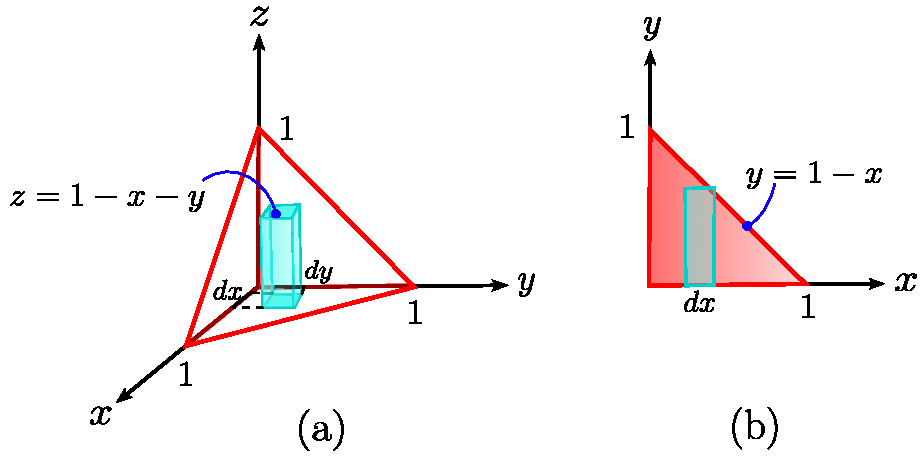
\includegraphics[scale = 0.7]{Figuras/Ej-Integral-Volumen-2.pdf}
        \caption{En (a) el tetraedro y en (b) la proyección  del tetraedro en el plano $xy$ en conjunto con el paralelepípedo y el rectángulo para ayudar a ver los límites de integración.}
        \label{fig:Ej-Int_Volumen-2}
    \end{figure}

    Por lo tanto,
    \begin{align*}
        \iiint_V x^2 \,dV &= \int_0^1 \left(\int_0^{1-x} \left(\int_0^{1-x-y} x^2 \,dz \right) dy \right) dx \\
        &= \int_0^1 \left(\int_0^{1-x} \left.  x^2 z \right|_{z=0}^{z = 1-x-y} dy \right) dx \\
        &= \int_0^1 \left(\int_0^{1-x} x^2(1-x-y) dy \right) dx \\
        &= \int_0^1 x^2 \left[ (1-x)y - \frac{y^2}{2} \right]_{y = 0}^{y = 1-x} dx  \\
        &= \int_0^1 x^2  (1-x)^2- x^2 \frac{(1-x)^2}{2}  \,dx \\
        &= \frac{1}{2} \int_0^1 x^2(1-x)^2 \,dx \\
        &= \frac{1}{60}.
    \end{align*}

    Queda como ejercicio para el lector verificar que para los órdenes de integración:
    \begin{enumerate}
        \item $dxdydz$:
        $$V: \left\{ \begin{array}{ccccl}
             0 & \leq & x & \leq & 1-z-y  \\
             0 & \leq & y & \leq & 1-z \\
             0 & \leq & z & \leq & 1
        \end{array} \right. .$$

        \item $dydzdx$:
        $$V: \left\{ \begin{array}{ccccl}
             0 & \leq & y & \leq & 1-z-x  \\
             0 & \leq & z & \leq & 1-x \\
             0 & \leq & x & \leq &1
        \end{array} \right. .$$
    \end{enumerate}

    se obtiene el mismo valor.
\end{ejemplo}

\subsection{Teoremas integrales}

\begin{teorema}[de Gauss] \label{Gauss}
    Sea $V$ una región limitada por una superficie $S$ suave y cerrada, tal que se le pueda atribuir una orientación en cada punto. Si $\vec{F}$ es un campo vectorial de clase $C^1$ sobre un abierto que contiene a $V$ y $\hat{n}$ la orientación dada por la normal exterior a $S$. Entonces,
    \begin{equation*}
    \boxed{\iint_S \vec{F} \cdot \hat{n}dS = \iiint_V \vec{\nabla} \cdot \vec{F} dV} 
    \end{equation*}
\end{teorema}

\begin{teorema}[de Stokes] \label{Stokes}
    Sea $S$ una superficie suave orientada con un vector unitario $\hat{n}$ y supongamos que $S$ tiene un borde $C$, que es una curva cerrada, lisa a trozos (seccionalmente suave), cuya orientación es compatible con la de $S$.

    Si $\vec{F}$ es un campo vectorial de clase $C^1$ en un abierto que contiene a $S$ y su frontera $C$, se verifica:
    \begin{equation*}
    \boxed{\int_C \vec{F} \cdot d\vec{r} = \iint_S (\vec{\nabla} \times \vec{F}) \cdot \hat{n}dS}
    \end{equation*}
\end{teorema}

\section{Coordenadas curvilíneas}

Las \textbf{coordenadas curvilíneas} son sistemas de coordenadas en el espacio Euclidiano donde las líneas pueden ser curvas. Estas coordenadas pueden ser obtenidas a partir del sistema de coordenadas cartesiano mediante una transformación que es \underline{invertible} en cada punto. Ésto significa que podemos convertir un punto dado en coordenadas cartesianas a un sistema curvilíneo y viceversa.

\subsection{Coordenadas esféricas}

Un punto $P$ en el espacio tridimensional euclídeo, en coordenadas esféricas, se especifica mediante tres coordenadas: $(r, \theta, \varphi)$, donde $r$ es la distancia desde el origen al punto $P$, $\theta$ es el ángulo que se forma entre el semieje $z$ positivo y el vector, y $\varphi$ es el ángulo que se forma entre el semieje $x$ positivo y la proyección del vector en el plano $xy$, ver figura \ref{fig:Coordenadas-Esfericas}.

\begin{figure}[H]
    \centering
    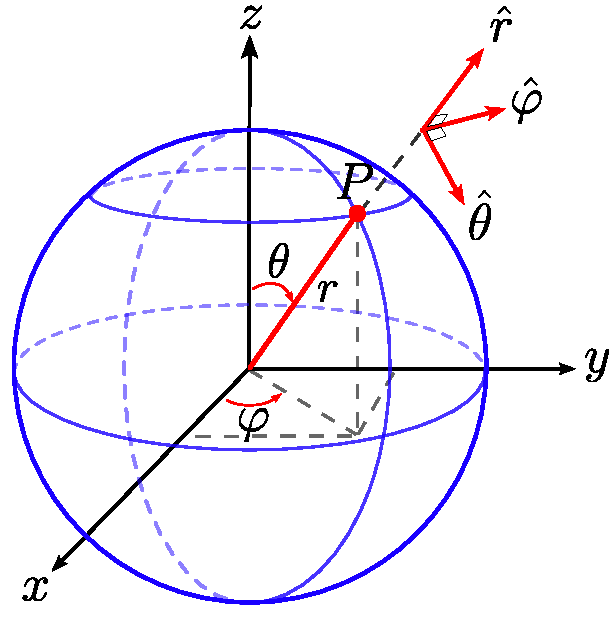
\includegraphics[scale = 0.65]{Figuras/Coordenadas-Esfericas.pdf}
    \caption{Coordenadas esféricas $(r,\theta,\varphi)$ en conjunto con sus vectores unitarios.}
    \label{fig:Coordenadas-Esfericas}
\end{figure}

Si se restringen las coordenadas $r$, $\theta$ y $\varphi$ a
$$r \geq 0, \quad 0 \leq \theta \leq \pi, \quad 0 \leq \varphi < 2\pi,$$

se puede obtener todo punto $P \in \mathbb{R}^3$. Gracias a las restricciones, se tiene la siguiente conversión de coordenadas esféricas a cartesianas:
\begin{align*}
    x &= r \sin \theta \cos \varphi,\\
    y &= r \sin \theta \sin \varphi ,\\
    z &= r \cos \theta,
\end{align*}

y de cartesianas a esféricas: \footnote{Recuerde que el recorrido de la función $\arccos(x)$ es $[-\pi/2, \pi/2]$ y de la función $\arctan(x)$ es $]-\pi/2, \pi/2[$, entonces dependiendo donde se ubique $(x,y,z)$ se tendrá que sumar un múltiplo de $\pi$.}
\begin{align*}
    r &= \sqrt{x^2+y^2+z^2}, \\
    \theta &= \arccos \left(\frac{z}{r} \right) = \arccos \left( \frac{z}{\sqrt{x^2+y^2+z^2}} \right), \\
    \varphi &= \arctan \left( \frac{y}{x} \right).
\end{align*}

La base ortonormal en el sistema de coordenadas esféricas la forman los vectores $\hat{r}, \hat{\theta}$ y $\hat{\varphi}$, ver figura \ref{fig:Coordenadas-Esfericas}, los cuales apuntan en el sentido de crecimiento de las correspondientes coordenadas y verifican:
$$\hat{\theta} \times \hat{\varphi} = \hat{r}.$$

Al igual que toda base, todo vector $\Vec{A}$ puede ser expresado en términos de ellos, en la forma usual:
$$\Vec{A} = A_r \hat{r} + A_{\theta} \hat{\theta} + A_{\varphi} \hat{\varphi}.$$

A partir de la transformación de coordenadas, el vector posición toma la forma
$$\Vec{x} = x \,\hat{\imath} + y \,\hat{\jmath} + z \,\hat{k} = r \sin \theta \cos \varphi \,\hat{\imath} + r \sin \theta \sin \varphi \,\hat{\jmath} + r \cos\theta \,\hat{k}.$$

Así, los vectores unitarios pueden ser expresados en la base cartesiana $\{\hat{\imath}, \hat{\jmath}, \hat{k}\}$, como sigue.
\begin{align*}
    \hat{r} &= \frac{1}{\norm{\frac{\partial \Vec{x}}{\partial r}}}\frac{\partial \Vec{x}}{\partial r} = \sin \theta \cos \varphi \,\hat{\imath} + \sin \theta \sin \varphi \,\hat{\jmath} + \cos \theta \,\hat{k} \\,
    \hat{\theta} &= \frac{1}{\norm{\frac{\partial \Vec{x}}{\partial \theta}}}\frac{\partial \Vec{x}}{\partial \theta} = \cos \theta \cos \varphi \,\hat{\imath} + \cos \theta \sin \varphi \,\hat{\jmath} - \sin \theta   \,\hat{k},  \\
    \hat{\varphi} &= \frac{1}{\norm{\frac{\partial \Vec{x}}{\partial \varphi}}}\frac{\partial \Vec{x}}{\partial \varphi} = - \sin \varphi \,\hat{\imath} + \cos \varphi \,\hat{\jmath} .
\end{align*}

\textbf{Nota:} Dado que la derivada parcial con respecto a una coordenada considera el resto como constantes, el vector unitario es tangente a la curva que se genera manteniendo dichas coordenadas constantes. Por ejemplo, $\hat{r}$ es tangente a la curva que se genera al considerar $\theta$ y $\varphi$ constantes, ésto es, un rayo que parte del origen.

Observe que los vectores unitarios $\hat{r}, \hat{\theta}$ y $\hat{\varphi}$ no son constantes, a diferencia de los vectores unitarios cartesianos, de hecho $\hat{r} = \hat{r}(\theta,\varphi)$, $\hat{\theta} = \hat{\theta}(\theta,\varphi)$ y $\hat{\varphi} = \hat{\varphi}(\theta,\varphi)$. Por lo tanto, al momento de derivar o integrar hay que tener cuidado.

Por lo anterior, el vector posición de un punto $P$ con coordenadas $(r, \theta, \varphi)$ es 
\begin{equation*}
\vec{x} = r \hat{r}
\end{equation*}

Se puede demostrar que los vectores unitarios cartesianos se pueden escribir como combinación lineal de los vectores unitarios esféricos, a saber,
\begin{align*}
    \hat{\imath} &= \sin \theta \cos \varphi \,\hat{r} + \cos \theta \cos \varphi \,\hat{\theta} - \sin \varphi \,\hat{\varphi},\\
    \hat{\jmath} &= \sin \theta \sin\varphi \,\hat{r} + \cos \theta \sin \varphi \,\hat{\theta} + \cos \varphi \,\hat{\varphi}, \\
    \hat{k} &= \cos \theta \,\hat{r} - \sin \theta \,\hat{\theta}.
\end{align*}

Consideremos un punto $(r,\theta, \varphi)$ en el espacio, nos desplazamos infinitesimalmente en las direcciones $\hat{r}$, $\hat{\theta}$ y $\hat{\varphi}$ al punto $(r + dr, \theta + d\theta, \varphi + d\varphi)$. Estamos tentados a escribir, al igual que en coordenadas cartesianas, el elemento infinitesimal de desplazamiento (o de línea) como $d \Vec{x} = dr \hat{r} + d\theta \hat{\theta} + d\varphi \hat{\varphi}$ (\textcolor{red}{NO!!!!!!!}), lo cual es incorrecto, incluso dimensionalmente es inconsistente, pues $d\theta$ y $d\varphi$ no tienen unidades de longitud. Debemos analizar por separado los elementos infinitesimales de longitud en cada dirección.

Un desplazamiento en la dirección $\hat{r}$ es simplemente $dr$ (figura \ref{fig:Elemento-Esferica}-(a)), así 
$$dx_r = dr.$$

Por otro lado, un elemento infinitesimal de longitud en la dirección $\hat{\theta}$ (figura \ref{fig:Elemento-Esferica}-(b)) es
$$dx_{\theta} = r \,d\theta.$$

Similarmente, un elemento infinitesimal de longitud en la dirección $\hat{\varphi}$ (figura \ref{fig:Elemento-Esferica}-(c)) es
$$dx_{\varphi} = r \sin\theta \,d\varphi.$$

Por lo tanto, el desplazamiento infinitesimal general está dado por
\begin{shaded}
    $$d\Vec{x} = dr \, \hat{r} + r \,d\theta \,\hat{\theta} + r \sin \theta \,d\varphi \,\hat{\varphi}.$$
\end{shaded}

\begin{figure}[H]
    \centering
    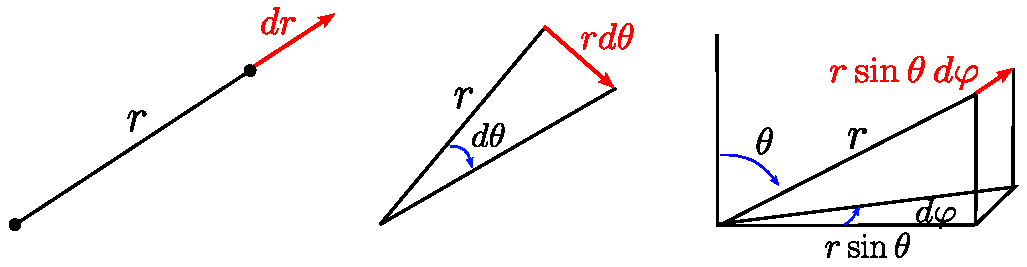
\includegraphics[scale = 0.7]{Figuras/Elemento-Esferica.pdf}
    \caption{}
    \label{fig:Elemento-Esferica}
\end{figure}

\textbf{Observación:} Ésto juega el mismo rol (en las integrales de línea, por ejemplo) de $d\Vec{x} = dx \,\hat{\imath} + dy\,\hat{\jmath} + dz \,\hat{k}$ en las coordenadas cartesianas.

El elemento infinitesimal de volumen, en coordenadas esféricas, es el producto de los tres desplazamientos infinitesimales:
\begin{shaded}
    $$dV = r^2 \sin \theta \,dr\,d\theta\,d\varphi,$$
\end{shaded}

lo cual corresponde al volumen del paralelepípedo formado por los vectores: $dr \,\hat{r}$, $r \,d\theta \, \hat{\theta}$ y $r \sin \theta \,d\varphi \, \hat{\varphi}$.

No existe una expresión general para los elementos de superficie $d\Vec{S}$, ya que estos dependen de la orientación de la superficie. Para obtenerlos uno tiene que analizar la geometría para cada caso. En la figura \ref{fig:Vol-Esfericas}, se encuentran representados los diferentes elementos infinitesimales que se pueden obtener. Para el caso de los elementos infinitesimales  de superficie, se tienen tres casos:
\begin{shaded}
  \begin{equation*}
d\vec{S}_r = r^2 \sen \theta\, d\theta\, d\varphi \,\hat{r} ,\quad d\vec{S}_{\theta} = r \sin\theta \,dr \,d \varphi \,\hat{\theta}, \quad  d\vec{S}_{\varphi} = r \,dr\, d\theta \,\hat{\varphi}.
\end{equation*}  
\end{shaded}

\begin{ejemplo}
    El volumen de una esfera (maciza) de radio $R$ es 
    \begin{align*}
        V = \int dV &= \int_0^{2\pi} \left( \int_0^{\pi} \left( \int_0^R r^2 \sin \theta \,dr \right)d\theta \right) d\varphi \\
        &= \left( \int_0^{2\pi} d\varphi\right) \left(\int_0^{\pi} \sin \theta \,d\theta \right) \left(\int_0^R r^2 \,dr \right) \\
        &= (2\pi) (2) \left(\frac{R^3}{3} \right) = \frac{4}{3} \pi R^3.
    \end{align*}
\end{ejemplo}

\begin{figure}[H]
    \centering
    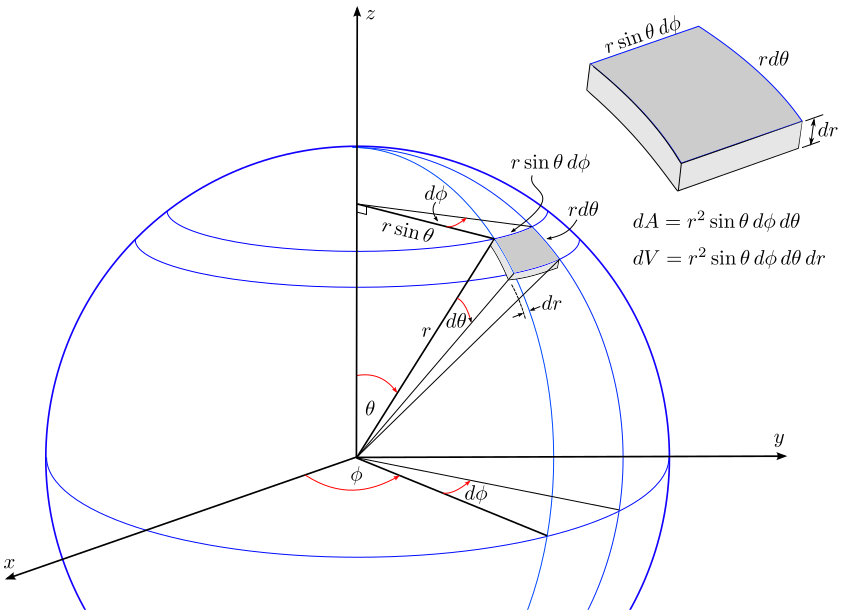
\includegraphics[scale = 0.5]{Figuras/volumenesfericas.png}
    \caption{Elementos infinitesimales en coordenadas esféricas. Recuperado de \cite{Alvarez} en la pág. 35.}
    \label{fig:Vol-Esfericas}
\end{figure}

\subsection{Coordenadas cilíndricas}

Un punto $P$ en el espacio tridimensional euclídeo, en coordenadas cilíndricas, se especifica mediante tres coordenadas: $(\rho, \varphi, z)$, donde $\rho$ es la distancia a $P$ desde el eje $z$, $\varphi$ es el ángulo que se forma entre el semieje $x$ positivo y la proyección del vector en el plano $xy$, y $z$ es la misma coordenada que en cartesianas, ver figura \ref{fig:Coordenadas-Cilindricas}.

\begin{figure}[H]
    \centering
    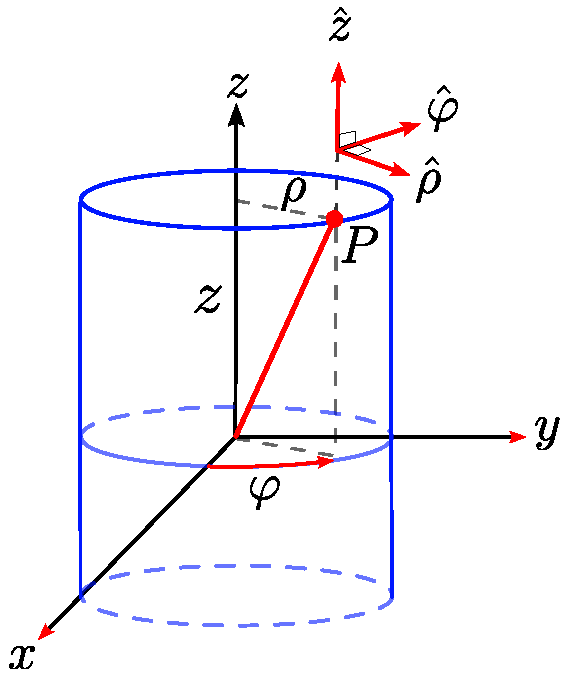
\includegraphics[scale = 0.65]{Figuras/Coordenadas-Cilindricas.pdf}
    \caption{Coordenadas cilíndricas $(\rho,\varphi, z)$ en conjunto con sus vectores unitarios.}
    \label{fig:Coordenadas-Cilindricas}
\end{figure}

Si se restringen las coordenadas $\rho$, $\varphi$ y $z$ a
$$\rho \geq 0, \quad 0 \leq \varphi < 2\pi, \quad -\infty < z < \infty,$$

se puede obtener todo punto $P \in \mathbb{R}^3$. Gracias a las restricciones, se tiene la siguiente conversión de coordenadas cilíndricas a cartesianas:
\begin{align*}
    x &= \rho \cos \varphi,\\
    y &= \rho \sin \varphi ,\\
    z &= z,
\end{align*}

y de cartesianas a cilíndricas:
\begin{align*}
    \rho &= \sqrt{x^2+y^2}, \\
    \varphi &= \arctan \left( \frac{y}{x} \right), \\
    z &= z .
\end{align*}

La base ortonormal en el sistema de coordenadas cilíndricas la forman los vectores $\hat{\rho}, \hat{\varphi}$ y $\hat{k}$, ver figura \ref{fig:Coordenadas-Cilindricas}, que verifican:
$$\hat{\rho} \times \hat{\varphi} = \hat{k}.$$

Al igual que toda base, todo vector $\Vec{A}$ puede ser expresado en términos de ellos, en la forma usual:
$$\Vec{A} = A_{\rho} \hat{\rho}  + A_{\varphi} \hat{\varphi} + A_z \hat{k}.$$

A partir de la transformación de coordenadas, el vector posición toma la forma
$$\Vec{x} = x \,\hat{\imath} + y \,\hat{\jmath} + z \,\hat{k} = \rho \cos \varphi \,\hat{\imath} + \rho \sin \varphi \,\hat{\jmath} + z \,\hat{k}.$$

Así, los vectores unitarios pueden ser expresados en la base cartesiana $\{\hat{\imath}, \hat{\jmath}, \hat{k}\}$, como sigue.
\begin{align*}
    \hat{\rho} &= \frac{1}{\norm{\frac{\partial \Vec{x}}{\partial \rho}}}\frac{\partial \Vec{x}}{\partial \rho} = \cos \varphi \,\hat{\imath} + \sin \varphi \,\hat{\jmath} \\,
    \hat{\varphi} &= \frac{1}{\norm{\frac{\partial \Vec{x}}{\partial \varphi}}}\frac{\partial \Vec{x}}{\partial \varphi} = - \sin \varphi \,\hat{\imath} + \cos \varphi \, \hat{\jmath},  \\
    \hat{k} &= \frac{1}{\norm{\frac{\partial \Vec{x}}{\partial z}}}\frac{\partial \Vec{x}}{\partial z} = \hat{k} .
\end{align*}

Por lo anterior, el vector posición de un punto $P$ con coordenadas $(\rho, \varphi,z)$ es 
\begin{equation*}
\vec{x} = \rho \hat{\rho} + z \hat{k}.
\end{equation*}

Se puede demostrar que los vectores unitarios cartesianos se pueden escribir como combinación lineal de los vectores unitarios cilíndricos, a saber,
\begin{align*}
    \hat{\imath} &= \cos \varphi \,\hat{\rho} - \sin \varphi \, \hat{\varphi}, \\
    \hat{\jmath} &= \sin\varphi \, \hat{\rho} + \cos \varphi \,\hat{\varphi}.
\end{align*}

Consideremos un punto $(\rho, \varphi, z)$ en el espacio, nos desplazamos infinitesimalmente en las direcciones $\hat{\rho}$, $\hat{\varphi}$ y $\hat{k}$ al punto $(\rho + d\rho, \varphi + d\varphi, z + dz)$. A partir de la figura \ref{fig:Elemento-Cilindrica}, se tiene que los elementos infinitesimales de longitud en las direcciones $\hat{\rho}$, $\hat{\varphi}$ y $\hat{k}$, están dados, respectivamente, por
$$dx_{\rho} = d\rho, \quad dx_{\varphi} = \rho \,d\varphi, \quad dx_z = dz.$$

Por lo tanto, el desplazamiento infinitesimal general está dado por
\begin{shaded}
    $$d\Vec{x} = d\rho \, \hat{\rho} + \rho \,d\varphi \,\hat{\varphi} + dz \,\hat{k}.$$
\end{shaded}

\begin{figure}[H]
    \centering
    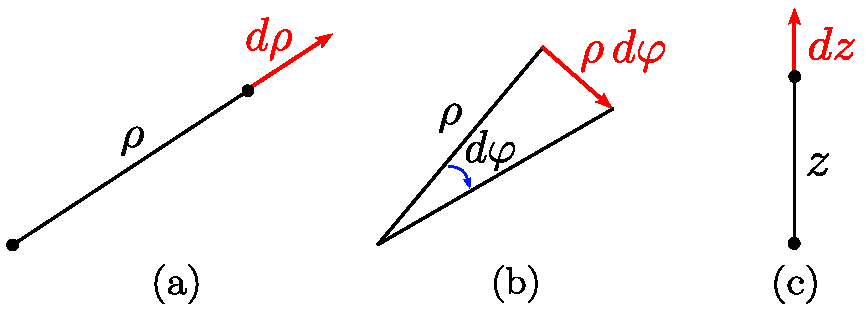
\includegraphics[scale = 0.7]{Figuras/Elemento-Cilindrica.pdf}
    \caption{}
    \label{fig:Elemento-Cilindrica}
\end{figure}

El elemento infinitesimal de volumen, en coordenadas cilíndricas, es el producto de los tres desplazamientos infinitesimales:
\begin{shaded}
    $$dV = \rho \,d\rho\,d\varphi\,dz,$$
\end{shaded}

lo cual corresponde al volumen del paralelepípedo formado por los vectores: $d\rho \hat{\rho}$, $\rho \,d\varphi \, \hat{\varphi}$ y $dz \, \hat{k}$.

 En la figura \ref{fig:Vol-Cilindricas}, se encuentran representados los diferentes elementos infinitesimales que se pueden obtener. Para el caso de los elementos infinitesimales  de superficie, se tienen tres casos:
\begin{shaded}
\begin{equation*}
d\vec{S}_{\rho} = \rho \,d\varphi \,dz \,\hat{\rho},\quad d\vec{S}_{z} = \rho \,d\varphi\, d\rho \,\hat{k},\quad d\vec{S}_{\varphi} = d\rho\, dz \,\hat{\varphi}.
\end{equation*}  
\end{shaded}

\begin{figure}[H]
    \centering
    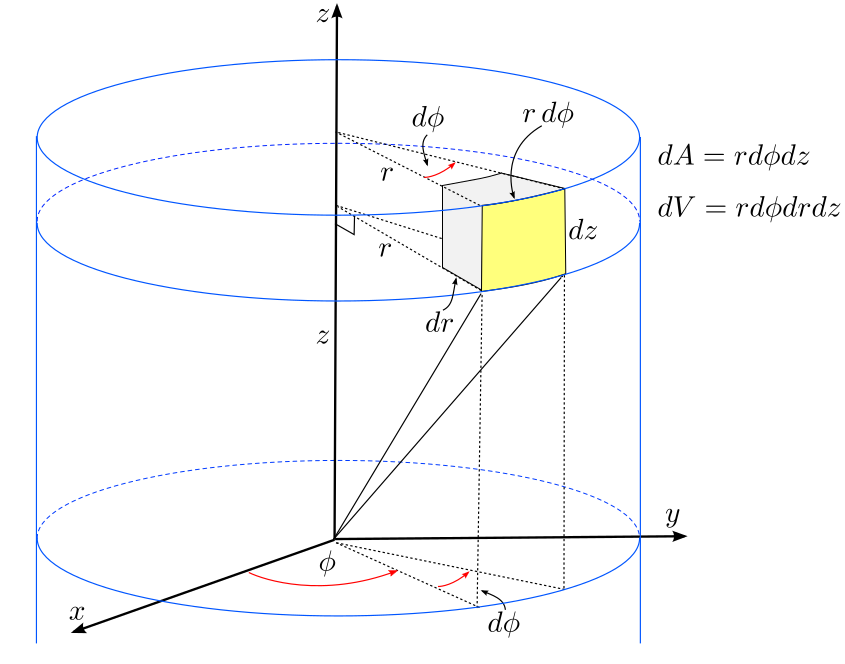
\includegraphics[scale = 0.4]{Figuras/Volumen-Cilindricas.png}
    \caption{Elementos infinitesimales en coordenadas cilíndricas donde se ha representado $\rho \to r$. Recuperado de \cite{Alvarez} en la pág. 37.}
    \label{fig:Vol-Cilindricas}
\end{figure}

\section{Operadores en coordenadas curvilíneas}

En la sección \ref{Operadores} definimos los operadores vectoriales en coordenadas cartesianas. Ahora veremos la forma que tienen en coordenadas esféricas y cilíndricas.

Sea el campo escalar diferenciable $f$ y el campo vectorial diferenciable $\vec{F}$ de componentes $F_{\rho}, F_{\varphi}, F_z$ en coordenadas cilíndricas y de componentes $F_r, F_{\theta}, F_{\varphi}$  en coordenadas esféricas.

\begin{itemize}
\item[i)] El \textbf{gradiente} en coordenadas cilíndricas es
\begin{shaded}
    $$\vec{\nabla} f(\rho, \varphi,z) = \frac{\partial f}{\partial \rho} (\rho, \varphi, z) \hat{\rho} + \frac{1}{\rho}  \frac{\partial f}{\partial \varphi} (\rho, \varphi, z) \hat{\varphi} + \frac{\partial f}{\partial z} (\rho, \varphi, z) \hat{k}$$
\end{shaded}

y en coordenadas esféricas
\begin{shaded}
    $$\vec{\nabla} f(r, \theta,\varphi) = \frac{\partial f}{\partial r} (r, \theta, \varphi) \hat{r} + \frac{1}{r} \frac{\partial f}{\partial \theta}(r, \theta, \varphi) \hat{\theta} + \frac{1}{r\sin\theta}\frac{\partial f}{\partial \varphi}(r, \theta, \varphi) \hat{\varphi}.$$
\end{shaded}

\item[ii)] La \textbf{divergencia} en coordenadas cilíndricas es
\begin{shaded}
    $$\vec{\nabla} \cdot \vec{F}(\rho, \varphi,z) = \frac{1}{\rho} \frac{\partial(\rho F_{\rho})}{\partial \rho} + \frac{1}{\rho} \frac{\partial F{\varphi}}{\partial\varphi} + \frac{\partial F_z}{\partial z}$$
\end{shaded}

y en coordenadas esféricas
\begin{shaded}
    $$\vec{\nabla} \cdot \vec{F}(r,\theta, \varphi) = \frac{1}{r^2} \frac{\partial (r^2 F_r)}{\partial r} + \frac{1}{r\sin\theta} \frac{\partial (\sin\theta F_{\theta})}{\partial \theta} + \frac{1}{r\sin\theta} \frac{\partial F_{\varphi}}{\partial \varphi}.$$
\end{shaded}

\item[iii)] El \textbf{rotacional} en coordenadas cilíndricas es
\begin{shaded}
    $$\vec{\nabla} \times \vec{F} = \left( \frac{1}{\rho} \frac{\partial F_z}{\partial \varphi} - \frac{\partial F_{\varphi}}{\partial z}\right) \hat{\rho} + \left( \frac{\partial F_{\rho}}{\partial z} - \frac{\partial F_z}{\partial \rho}\right) \hat{\varphi} + \frac{1}{\rho} \left[ \frac{\partial (\rho F_{\varphi})}{\partial \rho} - \frac{\partial F_{\rho}}{\partial \varphi} \right] \hat{k}.$$
\end{shaded}

y en coordenadas esféricas
\begin{shaded}
    $$\vec{\nabla} \times \vec{F} = \frac{1}{r \sin \theta} \left[ \frac{\partial (\sin\theta F_{\varphi})}{\partial \theta} - \frac{\partial F_{\theta}}{\partial \varphi} \right]\hat{r} + \frac{1}{r} \left[ \frac{1}{\sin \theta} \frac{\partial F_r}{\partial \varphi} - \frac{\partial (r F_{\varphi})}{\partial r} \right] \hat{\theta} 
     + \frac{1}{r} \left[ \frac{\partial (rF_{\theta})}{\partial r} - \frac{\partial F_r}{\partial \theta} \right] \hat{\varphi}.$$
\end{shaded}


\item[iv)] El \textbf{laplaciano} en coordenadas cilíndricas es
\begin{shaded}
    $$\nabla^2 f(\rho, \varphi,z) = \frac{1}{\rho} \frac{\partial}{\partial \rho} \left(\rho \frac{\partial f}{\partial \rho} \right) + \frac{1}{\rho^2} \frac{\partial^2 f}{\partial \varphi^2}  + \frac{\partial^2 f}{\partial z^2}$$
\end{shaded}

y en coordenadas esféricas
\begin{shaded}
    $$\nabla^2 f(r,\theta,\varphi) = \frac{1}{r^2} \frac{\partial}{\partial r^2} \left( r^2 \frac{\partial f}{\partial r} \right) + \frac{1}{r^2 \sin\theta} \frac{\partial}{\partial \theta} \left( \sin \theta \frac{\partial f}{\partial \theta}\right) + \frac{1}{r^2 \sin^2\theta} \frac{\partial^2 f}{\partial \varphi^2}.$$
\end{shaded}
\end{itemize}





\chapter{Electrostática}

En la naturaliza existen 4 interacciones fundamentales:
\begin{enumerate}
\item Interacción gravitatoria.
\item Fuerza electromagnética.
\item Fuerza nuclear fuerte.
\item Fuerza nuclear débil.
\end{enumerate}

En este curso estudiaremos la segunda, que abarca tanto la fuerza eléctrica como la fuerza magnética.  

Entendemos por \textbf{electromagnetismo} al estudio de los fenómenos eléctricos y magnéticos, los cuales (de forma preliminar) diremos que son producidos por \textit{cargas eléctricas} en reposo o en movimiento.

\myrule{to reversed}{to reversed}

\textbf{Un poco de historia...}

La existencia de la interacción eléctrica fue registrada hace 2.000 años por el griego \textit{Tales de Mileto}, quien observó que un pedazo de ámbar al ser frotado con un un paño, atraía pedacitos de hojas secas. De hecho, la palabra “electricidad” viene del vocablo griego ámbar  (\textbf{elektron}).

\myrule{to reversed}{to reversed}

El electromagnetismo se puede dividir en diferentes ramas tales como: electrostática, circuitería, magnetostática, electrodinámica, \dots

En este capítulo estudiaremos la \textbf{electrostática}, la cual estudia el fenómeno que ocurre cuando las interacciones entre cargas eléctricas están en reposo (o casi).

\section{Carga eléctrica} 

La \textbf{carga eléctrica} es un atributo o propiedad de la materia tan fundamental como la masa, y se hace presente en las partículas  de los átomos constituyentes. 

Existen dos tipos de cargas, las cuales se designan como \textcolor{blue}{positiva} ($+$) y \textcolor{red}{negativa} ($-$). La existencia de estas cargas se observa en el siguiente experimento:

\begin{enumerate}
\item Se frota una barra de vidrio con un paño de seda. 

\item Se frota una varilla de baquelita con un paño de seda.

\begin{figure}[H]
    \centering
    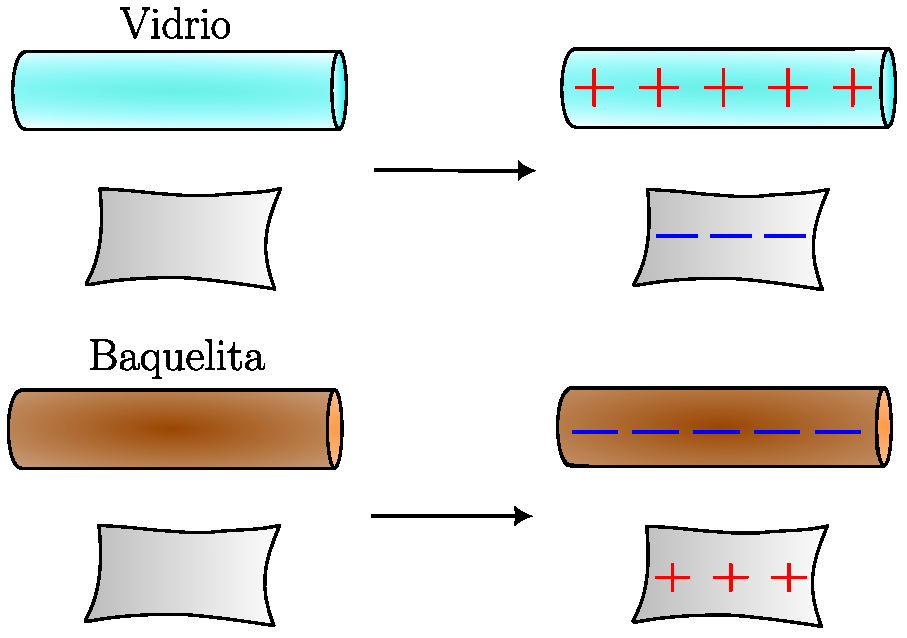
\includegraphics[scale = 0.5]{Figuras/Exp-Carga-Electrico.pdf}
    \caption{La varilla de vidrio queda cargada positivamente al ser frotada con el paño de seda. En cambio la varilla de baquelita queda con carga negativa.}
    \label{fig:Exp-Carga-Electrica1}
\end{figure}

\item Suspendemos la barra de vidrio cargada con un cordón, ver figura \ref{fig:Exp-Carga-Electrica2}-(a), y colocamos cerca una segunda barra de vidrio cargada, observamos que las dos barras se repelen entre sí. Sin embargo, si acercamos la varilla de baquelita, ésta atrae al extremo de la barra de vidrio suspendida, ver figura \ref{fig:Exp-Carga-Electrica2}-(b).

\end{enumerate}

Para poder explicar este resultado se propuso  que la barra de vidrio queda cargada y llamamos a esta carga \textit{positiva}. De igual manera queda cargada la varilla de baquelita y llamamos a esta carga \textit{negativa}.

Así, el paso 3. comprueba un importante principio:

\colorlet{shadecolor}{blue!10}
\begin{shaded}
\begin{center}
\textit{Cargas iguales se repelen y cargas distintas se atraen.}
\end{center}
\end{shaded}
\colorlet{shadecolor}{green!20}

\textbf{¿Pero cuál es el origen de la carga eléctrica?}

La materia está constituida de átomos. Cada átomo consiste de un núcleo, que contiene protones y neutrones, y este núcleo está rodeado por un cierto número de electrones. Los electrones tienen carga \textcolor{blue}{negativa} y los protones \textcolor{red}{positiva}, y los neutrones NO tienen carga eléctrica \footnote{No es adecuado decir carga cero o neutra.}. Los electrones pueden ser extraídos de los átomos mucho más fácilmente que los protones y neutrones. Por ello, el número de protones en el núcleo atómico determina la identidad de los elementos químicos.

La fuerza de repulsión o atracción entre dos cuerpos cargados dependerá de la  “cantidad neta de carga” que posean. Por carga neta se entiende la carga en exceso (positiva o negativa) que un cuerpo posee comparado con el mismo cuerpo neutro. Si se separan uno o más electrones, la estructura restante con carga positiva es un \textbf{ión positivo}. En el caso contrario que el átomo haya ganado uno o más electrones es un \textbf{ión negativo}. Esta ganancia o pérdida de electrones se conoce como \textbf{ionización}.

\begin{figure}[H]
    \centering
    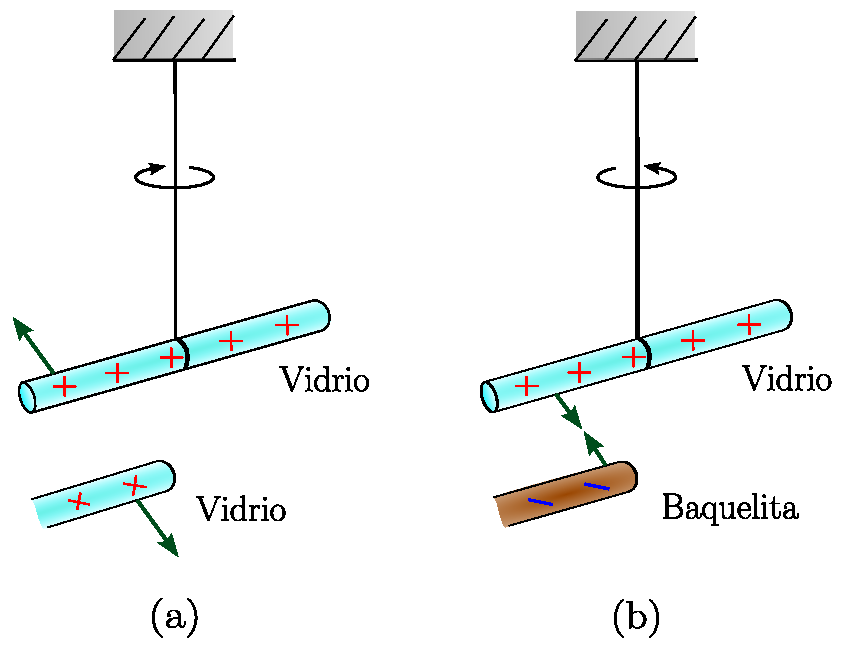
\includegraphics[scale = 0.7]{Figuras/Cargas-Opuestas-Iguales.pdf}
    \caption{(a) Dos varillas con cargas iguales se repelen entre sí. (b) Dos varillas con cargas opuestas se atraen mutuamente.}
    \label{fig:Exp-Carga-Electrica2}
\end{figure}

\subsection{Principios}

\subsubsection{Principio de cuantización de la carga}

Los experimentos demuestran además que la carga está \textbf{cuantizada}. Ésto quiere decir que la carga viene en múltiplos enteros de una carga elemental ($e$). En otras palabras, si un cuerpo tiene una carga neta $q$, entonces necesariamente se cumple:
\begin{equation*}
\boxed{q = \pm N e}
\end{equation*}

donde $N \in \mathbb{N}$ y $e$ es la \textbf{carga fundamental} que tiene un valor de \cite{CODATA}
\begin{equation*}
e = 1.602 176 634 \times 10^{-19} \, [C],
\end{equation*}

donde la unidad de carga es llamada \textbf{Coulomb} ($C$). Para nuestro caso, utilizaremos el valor $e = 1.602 \cdot 10^{-19} \, [C]$. Esto quiere decir que NO puede haber una carga más pequeña que $e$, la cual corresponde al valor absoluto de la carga del electrón.

\textbf{Observación:} La unidad de medida de la carga en el S.I es el Amperè segundo $[A\,s]$, donde $1 \, \mbox{Coulomb} \, = \,1 \,\mbox{Amperè\,segundo}$ y $1 \,[A] = 6.24150962915265 \cdot 10^{18}$ cargas elementales por segundo. Es decir, son necesarios $6 \times 10^{18}$ electrones para completar una carga de $-1.0 \,[C]$!!!

Para darse una idea del tamaño de las partículas que constituyen un átomo, se muestran en la tabla: las masas de los electrones, protones y neutrones junto con sus respectivas cargas \cite{Alvarez}. 

\begin{center}
 \begin{tabular}{ccc}
 \hline
 Partícula & Masa (kg) & Carga (C) \\ \hline
 electrón &   $9.11 \times 10^{-31}$ & $- 1.602 \times 10^{-19} ~ (-e)$ \\
 protón & $1.673 \times 10^{-27}$ & $+ 1.602 \times 10^{-19} ~(+e)$ \\
 neutrón & $1.675 \times 10^{-27}$ &  --- \\
 \hline 
 \end{tabular}
\end{center}

Se puede apreciar que $m_{\text{núcleo}} \approx 2.000 \, m_e$, es decir, el $99 \%$ de la masa del átomo es su núcleo. Además, la magnitud de la carga del electrón o del protón, en valor absoluto, son iguales.

\subsubsection{Principio de conservación de la carga}

Este principio establece que la carga neta de un sistema \textit{aislado} permanece constante, es decir,
\begin{equation*}
\sum_i q_i = cte.
\end{equation*}

Si un sistema parte con un número igual de cargas positivas y negativas, no se puede hacer nada para crear un exceso de carga negativa o positiva en el sistema a menos que traigamos una carga desde afuera del sistema (o quitar alguna carga del sistema).

\subsection{Tipos de materiales}

Las fuerzas entre dos objetos cargados pueden ser muy grandes. La mayoría de los objetos son eléctricamente neutros; tienen igual cantidad de cargas positivas que negativas.

Los materiales están divididos en tres categorías, dependiendo cuan fácilmente permiten el flujo de carga (ej. electrones) a lo largo de ellos. Éstos son:

\begin{itemize}
\item Los \textbf{Conductores} son cuerpos que, aunque estén neutros, tienen una enorme cantidad de \textit{electrones libres}, es decir, no ligados a los átomos, aptos para conducir la electricidad. Obviamente, la carga de estos electrones es neutralizada por la de los protones nucleares que están en los núcleos que supondremos fijos.

\textbf{Ejemplo:} Los metales y los electrolitos.

\item Los \textbf{aisladores} no conducen la electricidad ya que no poseen cargas libres, pero sus moléculas pueden polarizarse bajo influencia de una interacción eléctrica externa. Que se polaricen significa que estas moléculas, aunque neutras, pueden deformarse y/o orientarse, en mayor o menor grado. Esto confiere a los aisladores las denominadas \textit{propiedades dieléctricas} que estudiaremos después.

\textbf{Ejemplo:} Goma, madera, cerámica, plástico, \dots

\item Los \textbf{semiconductores}, que son la base de la electrónica actual, son cuerpos con propiedades de conducción intermedias entre los conductores y aisladores. En ellos se puede variar, con relativa facilidad, el número de cargas libres o portadores de electricidad.

\textbf{Ejemplo:} El silicio y el germanio.
\end{itemize}

\subsection{Métodos para cargar un objeto}

Hay tres maneras de cargar un objeto. 

\begin{enumerate}
\item Por \textbf{frotamiento}: esto es útil para cargar aisladores. Al comienzo de la sección se mostró un ejemplo de este método.

\item Por \textbf{conducción}: es útil para cargar metales y otros conductores. Si un objeto cargado toca a un conductor, una cantidad de carga será transferida entre el objeto y el conductor, de tal manera que el conductor quedará cargado con el mismo signo que la carga del objeto.

\item Por \textbf{inducción}: también es útil para cargar metales y otros conductores. 

 \textbf{Por ejemplo:} Acerquemos, sin tocar, una barra cargada negativamente a una esfera metálica neutra y aislada. Las cargas en la esfera se polarizan, es decir, los electrones se acumulan en un lado de la esfera, y del otro lado se produce deficiencia de electrones (carga +), pero la esfera sigue siendo neutra. Después, se conecta un alambre que permite que los electrones acumulados fluyan a tierra \footnote{ La Tierra es un conductor, y es tan
grande que actúa como una fuente prácticamente infinita de electrones adicionales o como un receptor de los electrones no deseados.}. Se desconecta el alambre de la esfera y se retira la barra con carga. Los electrones de la esfera se redistribuyen: la esfera en conjunto tiene una deficiencia de electrones (carga $+$), ver figura \ref{fig:Induccion-1}. 

En forma análoga, si se acerca una barra
cargada positivamente, se produce al final una esfera cargada negativamente,  ver figura \ref{fig:Induccion-2}.

\begin{figure}[H]
    \centering
    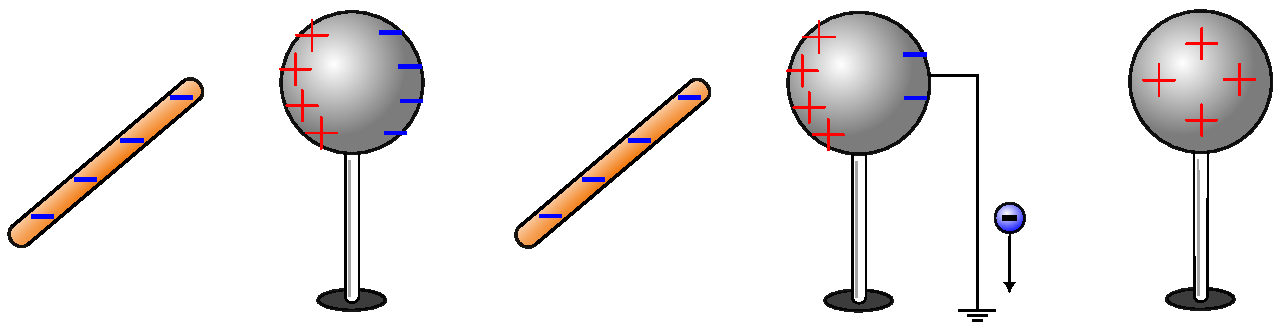
\includegraphics[scale = 0.5]{Figuras/Induccion-1.pdf}
    \caption{Inducción eléctrica, se acerca una barra con carga negativa a una esfera metálica, después de la conexión a tierra la esfera queda cargada positivamente.}
    \label{fig:Induccion-1}
\end{figure}

\begin{figure}[H]
    \centering
    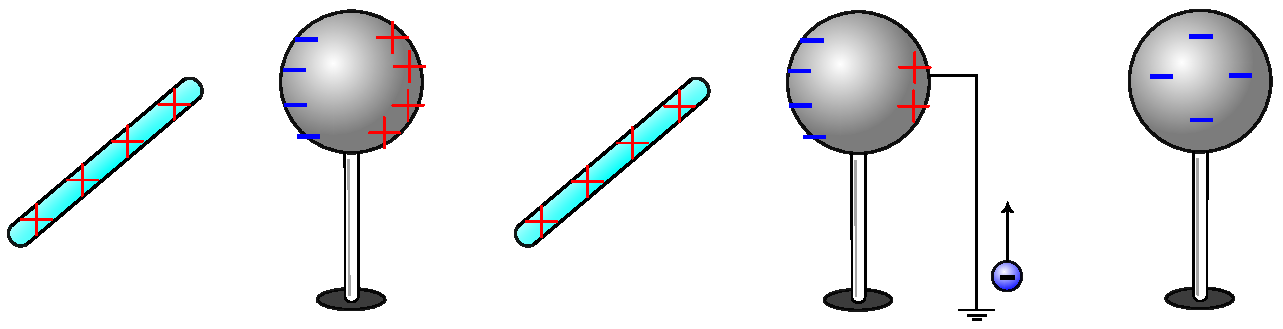
\includegraphics[scale = 0.5]{Figuras/Induccion-2.pdf}
    \caption{Inducción eléctrica, se acerca una barra con carga positiva a una esfera metálica, después de la conexión a tierra la esfera queda cargada negativamente.}
    \label{fig:Induccion-2}
\end{figure}
\end{enumerate}

\section{Ley de Coulomb}

\textbf{Charles Augustin Coulomb} (1736-1806) estudió en detalle, en 1785, las fuerzas de interacción de las partículas con carga eléctrica, utilizando una \textit{balanza de torsión} de Cavendish.

La \textit{balanza de torsión} consiste en una barra liviana colgada en su centro por un alambre de cuarzo (fibra de torsión) cuya constante elástica torsional $K$ se conoce, ver figura \ref{fig:Balanza-Torsion}.
En los extremos de la barra existen esferas de igual masa. Solo una de ellas posee carga eléctrica $q_1$, la cual se enfrenta a otra de carga eléctrica de igual signo $q_2$, fija en el laboratorio. 

Recordemos de los primeros cursos de Física que cuando una barra o varilla rota un ángulo $\theta$ a partir de su posición de equilibrio (en una balanza de torsión), el alambre se tuerce ejerciendo sobre la varilla un torque alrededor del centro que se opone al desplazamiento $\theta$ y de magnitud proporcional al ángulo, $\tau = K \theta$ (en magnitud), donde $K$ es la constante elástica de torsión. Luego de haber alcanzado el equilibrio rotacional, según los datos de la figura \ref{fig:Balanza-Torsion}-(b), se verifica que
$$Fb = K \theta \Rightarrow F = \frac{K\theta}{b},$$

donde $F b$ es el torque generado por la fuerza que ejerce la carga $q_2$ sobre $q_1$ con $b$  la distancia a la que se encuentra el punto $O$ de la recta de aplicación de la fuerza.

Experimentando con diferentes cargas y diferentes longitudes de barra, Coulomb encontró que para cargas puntuales, la magnitud de cada una de las fuerzas eléctricas con que interactúan 2 cargas puntuales es directamente proporcional al producto de las cargas e inversamente proporcional al cuadrado de la distancia que los separa con dirección según la linea que los une.
$$F \propto \frac{|q_1q_2|}{r^2} ~\Rightarrow ~ F = k \frac{|q_1q_2|}{r^2}.$$

El valor de la constante de proporcionalidad $k$ depende del sistema de unidades que se utilice. En el S.I.,
$$k = 8.987551787 \times 10^9 \,[Nm^2/C^2] \approx 9 \times 10^9 \, [Nm^2/C^2].$$

La constante $k$ se suele escribir como:
$$k = \frac{1}{4\pi \varepsilon_0}.$$

Luego, la \textbf{ley de Coulomb} se puede expresar de la siguiente manera
$$\boxed{F = \frac{1}{4\pi\varepsilon_0} \frac{|q_1q_2|}{r^2}}$$

donde las cargas están dadas por $q_1$ y $q_2$, la distancia de separación por $r$ y $\varepsilon_0 = 8.854 \times 10^{-12} \,[C^2/Nm^2]$ es la \textbf{permitividad eléctrica del espacio vacío} \cite{CODATA}.
\begin{figure}
        \centering
        \subfigure[]{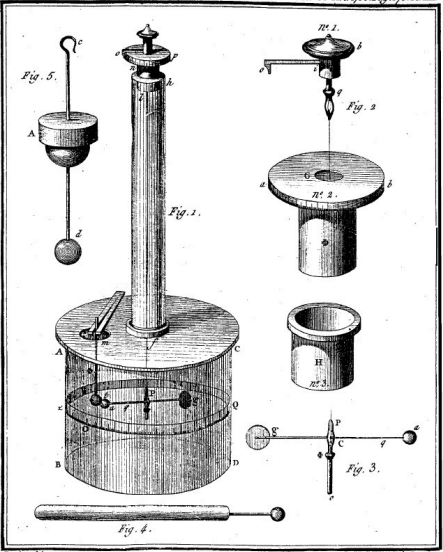
\includegraphics[width=0.5\textwidth]{Figuras/Exp_Coulomb.png}} \hspace{1cm}
        \subfigure[]{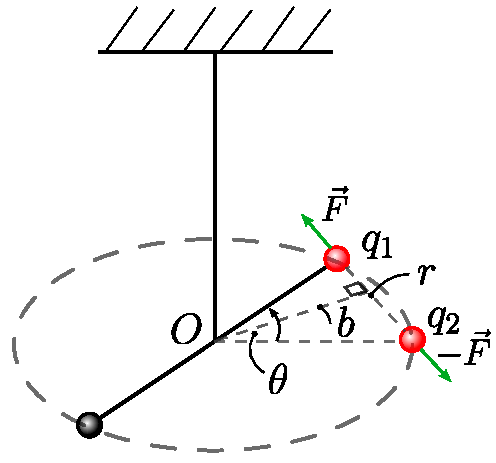
\includegraphics[width=0.4\textwidth]{Figuras/Esquema-Exp-Coulomb.pdf}} 
        \caption{En (a), el diagrama de la balanza de torsión de Coulomb. Recuperado de: Coulomb, C. A. (1788). \textit{Sur l'électricité et le magnétisme, premier mémoir}. En: Mémoires de l'Academie Royale des Sciences pour l’année 1785, Paris, pág 576. En (b), un dibujo esquemático de la balanza de torsión.}
        \label{fig:Balanza-Torsion}
    \end{figure}


\subsection*{Carácter vectorial}

Sean dos cargas puntuales, $q_1$ y $q_2$ en el vacío,  ubicadas mediante los
vectores posición $\vec{x}_1$ y $\vec{x}_2$ respecto a un sistema de referencia.

\begin{figure}[H]
    \centering
    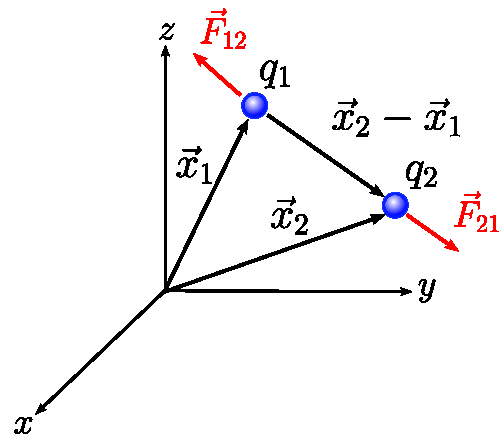
\includegraphics[scale = 0.7]{Figuras/Coulomb-Vectorial.pdf}
    \caption{Posición de las cargas puntuales.}
    \label{fig:Coulomb-Vectorial}
\end{figure}

 La ley de Coulomb establece que la fuerza que actúa sobre una partícula cargada $q_1$ debido a otra partícula cargada $q_2$ es:
 \begin{equation*}
 \vec{F}_{12} = \underbrace{\frac{1}{4\pi \varepsilon_0} \frac{q_1 q_2}{|\vec{x}_1 - \vec{x}_2|^2}}_{\text{Magnitud}} \underbrace{\frac{\vec{x}_1 - \vec{x}_2}{|\vec{x}_1 - \vec{x}_2|}}_{\text{Vector unitario}} = \frac{1}{4\pi \varepsilon_0} \frac{q_1 q_2}{|\vec{x}_1 - \vec{x}_2|^3} (\vec{x}_1 - \vec{x}_2).
 \end{equation*}

Análogamente, la fuerza que actúa sobre la partícula $q_2$ debido a otra
partícula cargada $q_1$ es:
\begin{equation*}
 \vec{F}_{21} = \underbrace{\frac{1}{4\pi \varepsilon_0} \frac{q_1 q_2}{|\vec{x}_2 - \vec{x}_1|^2}}_{\text{Magnitud}} \underbrace{\frac{\vec{x}_2 - \vec{x}_1}{|\vec{x}_2 - \vec{x}_1|}}_{\text{Vector unitario}} = - \frac{1}{4\pi \varepsilon_0} \frac{q_1 q_2}{|\vec{x}_1 - \vec{x}_2|^3} (\vec{x}_1 - \vec{x}_2).
 \end{equation*}

Note que se obedece la \textit{tercera ley de Newton}:
\begin{equation*}
\vec{F}_{12} = - \vec{F}_{21}. 
\end{equation*}

\textbf{Observación:} La ley de Coulomb para distancias muy cortas falla pues $F \to \infty$ cuando $r \to 0$. Si ésto es cierto, no existiría los núcleos atómicos.

\begin{ejemplo}
Calcule la fuerza que actúa sobre la carga $q_1 = -1,0 \times 10^{-6} \,[C]$ ubicada en el punto $(5,5) \,[cm]$ de un sistema cartesiano, y que es ejercida por una carga puntual $q_2 = 2,0 \times 10^{-6} \, [C]$, fija en el punto $(1,2) \,[cm]$. 


\begin{figure}[H]
    \centering
    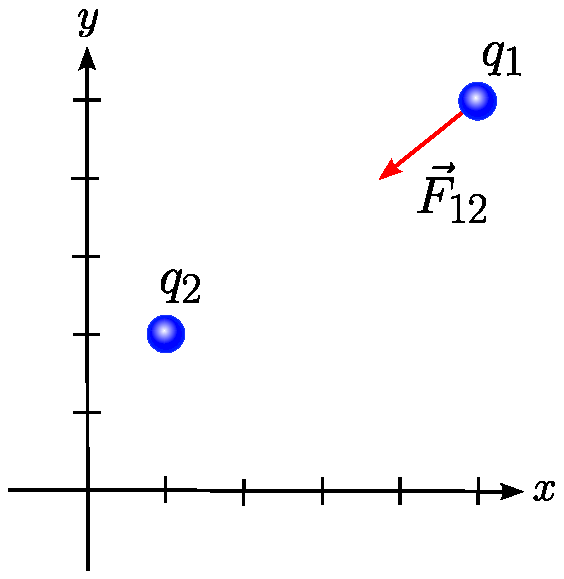
\includegraphics[scale = 0.5]{Figuras/Ej-Coulomb.pdf}
    \caption{Esquema.}
    \label{fig:Ej-Coulomb}
\end{figure}

\textbf{Solución:} Primero, se tiene que $\vec{x}_1 = (5 \,\hat{\imath} + 5 \, \hat{\jmath}) \,[cm]$ y $\vec{x}_2= (  \hat{\imath} + 2 \,\hat{\jmath}) \,[cm]$. Luego,
\begin{align*}
 \vec{x}_1 - \vec{x}_2 &= (5 \,\hat{\imath} + 5 \,\hat{\jmath}) - (\hat{\imath} + 2 \, \hat{\jmath}) \,[cm] = (4 \,\hat{\imath} + 3\,\hat{\jmath}) \,[cm] = (0.04 \,\hat{\imath} + 0.03\,\hat{\jmath}) \,[m], \\
|\vec{x}_1 - \vec{x}_2|^3 &= \left( \sqrt{4^2 + 3^2} \right)^3 = 125 \,[cm^3] = 1.25 \times 10^{-4} \, [m^3].   
\end{align*}

Entonces,
\begin{align*}
    \vec{F}_{12} &= k \frac{q_1q_2}{|\vec{x}_1 - \vec{x}_2|^3} (\vec{x}_1 - \vec{x}_2) \\
&= (9 \times 10^9) \cdot \frac{(-1\times 10^{-6})(2\times 10^{-6})}{1.25 \times 10^{-4}} (0.04 \,\hat{\imath} + 0.03 \,\hat{\jmath})  \, [N]\\
&= -5.76 \,\hat{\imath} - 4.32 \hat{\jmath} \,[N].
\end{align*}

\end{ejemplo}


\begin{ejemplo}
    Una cierta carga $Q$ es dividida en dos partes $q$ y $(Q-q)$, las cuales están separadas por una cierta distancia. ¿Cuál debe ser el valor de $q$ en términos de $Q$ para que la fuerza de repulsión sea máxima entre las dos cargas?

\textbf{Solución:} Designemos la distancia entre las dos cargas como $r$, entonces la magnitud de la fuerza es:
$$F = k \frac{|q||Q-q|}{r^2}.$$

Sabemos que las cargas tienen el mismo signo, así que podemos omitir los valores absolutos y asegurarnos de que $F$ sea positiva
$$F = k \frac{q(Q-q)}{r^2} = k \frac{qQ-q^2}{r^2}.$$

Para encontrar el valor de $q$ que hace máxima esta repulsión derivamos $F$ con respecto a $q$ e igualamos a cero:
$$\frac{dF}{dq} = k \frac{Q -2q}{r^2} = 0 \Rightarrow q = \frac{Q}{2}.$$

Es decir, la máxima repulsión se obtiene cuando dividimos $Q$ por la mitad.
\end{ejemplo}


 \section{Principio de superposición}

La ley de Coulomb, tal como la hemos expresado, describe sólo la interacción de 2 cargas puntuales. Los experimentos muestran que, cuando 2 cargas ejercen fuerzas simultáneamente sobre una tercera carga, la fuerza total que actúa sobre esa carga es la \textbf{suma vectorial} de las fuerzas que las 2 cargas ejercerían individualmente. Esta propiedad recibe el nombre de \textbf{principio de superposición de fuerzas}, la cual es válida para cualquier conjunto de cargas.

Por lo tanto, si sobre una partícula cargada $q_0$ actúan $n$ partículas cargadas $q_i$, entonces la fuerza total sobre $q_0$ es la suma vectorial de todas las fuerzas que sobre ella ejercen independientemente de todas las otras, es decir,
$$\vec{F}_0 = \sum_{i=1}^n \vec{F}_{0i} = \vec{F}_{01} + \vec{F}_{02} + \vec{F}_{03} + \cdots + \vec{F}_{0n},$$


o bien,
$$\vec{F}_0 = \frac{1}{4\pi \varepsilon_0} q_0 \sum_{i=1}^n \frac{q_i}{|\vec{x}_0 - \vec{x}_i|^3} (\vec{x}_0 - \vec{x}_i).$$

\begin{ejemplo}
   Tres cargas puntuales $q_0$, $q_1$ y $q_2$ desconocidas en magnitud y signo, se colocan, respectivamente, en los puntos $(0,0)$, $(a,0)$ y $(0,b)$ de un sistema cartesiano y son tales que ejercen sobre $q_0$ una fuerza de componentes conocidas, $F_x$ y $F_y$. Después se re-arreglan  estas cargas de modo que, aunque $q_0$ queda en $(0,0)$, $q_1$ ocupa el lugar de $q_2$ y ésta se traslada al punto $(-a,0)$, como en la figura \ref{fig:Ej-Principio-Superposicion}. Determine las nuevas componentes $F_x'$ y $F_y'$ de la fuerza sobre $q_0$ en función de $F_x$ y $F_y$.

\begin{figure}[H]
    \centering
    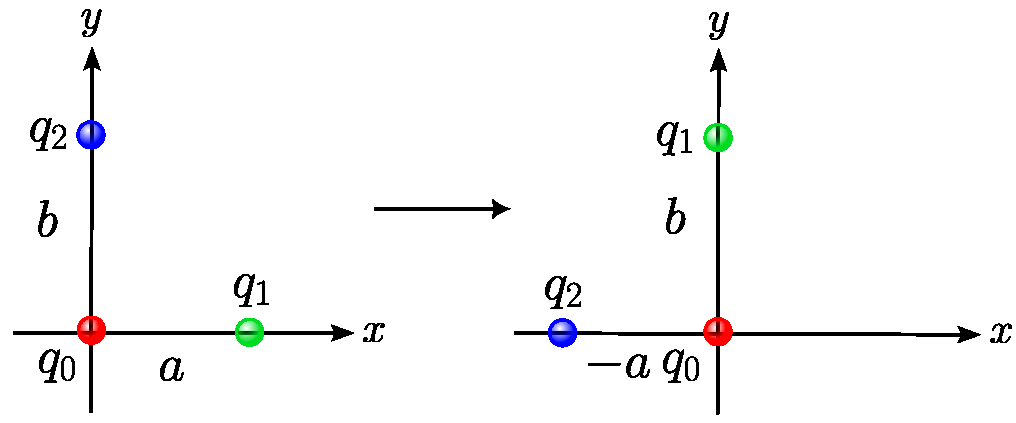
\includegraphics[scale = 0.6]{Figuras/Ej-Principio-Superposicion.pdf}
    \caption{Esquema.}
    \label{fig:Ej-Principio-Superposicion}
\end{figure}

\textbf{Solución:} Primero determinemos la fuerza neta sobre la carga $q_0$ antes del cambio de posición de las cargas.
\begin{align*}
    \vec{F}_0 &= \vec{F}_{01} + \vec{F}_{02} \\
&= k \frac{q_0q_1}{|\vec{x}_0 - \vec{x}_1|^3} (\vec{x}_0- \vec{x}_1) + k \frac{q_0q_2}{|\vec{x}_0 - \vec{x}_2|^3} (\vec{x}_0- \vec{x}_2) \\
&= k \frac{q_0q_1}{a^3} (-a \hat{\imath}) + k \frac{q_0q_2}{b^3} (-b \hat{\jmath}).
\end{align*}

Multiplicando por $\hat{\imath}$ y $\hat{\jmath}$, se obtienen las componentes (dato conocido):
\begin{align*}
    F_x &= - k \frac{q_0q_1}{a^2} \Rightarrow  q_1 = - \frac{F_x a^2}{k q_0}, \\
F_y &= - k \frac{q_0q_2}{b^2} \Rightarrow  q_2 = - \frac{F_y b^2}{k q_0}.
\end{align*}

Luego, cuando se cambia de posición las cargas, la nueva fuerza neta sobre la carga $q_0$ está dada por:
\begin{align*}
    \vec{F}_0 \,' &= \vec{F}_{01}\,' + \vec{F}_{02}\,' \\
&= k \frac{q_0q_1}{|\vec{x}_0 - \vec{x}_1\,'|^3} (\vec{x}_0- \vec{x}_1\,') + k \frac{q_0q_2}{|\vec{x}_0 - \vec{x}_2\,'|^3} (\vec{x}_0- \vec{x}_2\,') \\
&= k \frac{q_0q_1}{b^3} (-b \hat{\jmath}) + k \frac{q_0q_2}{a^3} (a \hat{\imath}).
\end{align*}

Reemplazando los valores de $q_1$ y $q_2$ en función de $F_x$ y $F_y$ encontrados.
$$\vec{F}_0\,' = - \frac{b^2}{a^2}F_y \hat{\imath} + \frac{a^2}{b^2} F_x \hat{\jmath}.$$

Por lo tanto,
$$F_x' = - \frac{b^2}{a^2}F_y ~~\mbox{y}~~ F_y' = \frac{a^2}{b^2} F_x.$$

\end{ejemplo}

\section{Ley de Coulomb para distribuciones continuas de carga}

Hemos visto que la carga eléctrica está cuantizada, pero desde el punto de vista macroscópico, puede considerarse que en los materiales las cargas pueden formar un continuo, pudiendo aplicarse en su análisis el Cálculo Diferencial.


Para aplicar la Ley de Coulomb a situaciones en que aparezcan estos materiales, se los subdivide formando elementos de carga y se aplica el principio de superposición, reemplazando la suma vectorial por una integral vectorial. Así la fuerza neta sobre una carga puntual es
$$\vec{F}_{neta} = \int d \vec{F}.$$

Por ejemplo, una carga puntual $q$ en presencia de una distribución continua de carga, donde $dq'$ es un elemento de carga de la distribución, la fuerza $d\Vec{F}$ que experimenta $q$ debido a $dq'$ es

\begin{figure}[H]
    \centering
    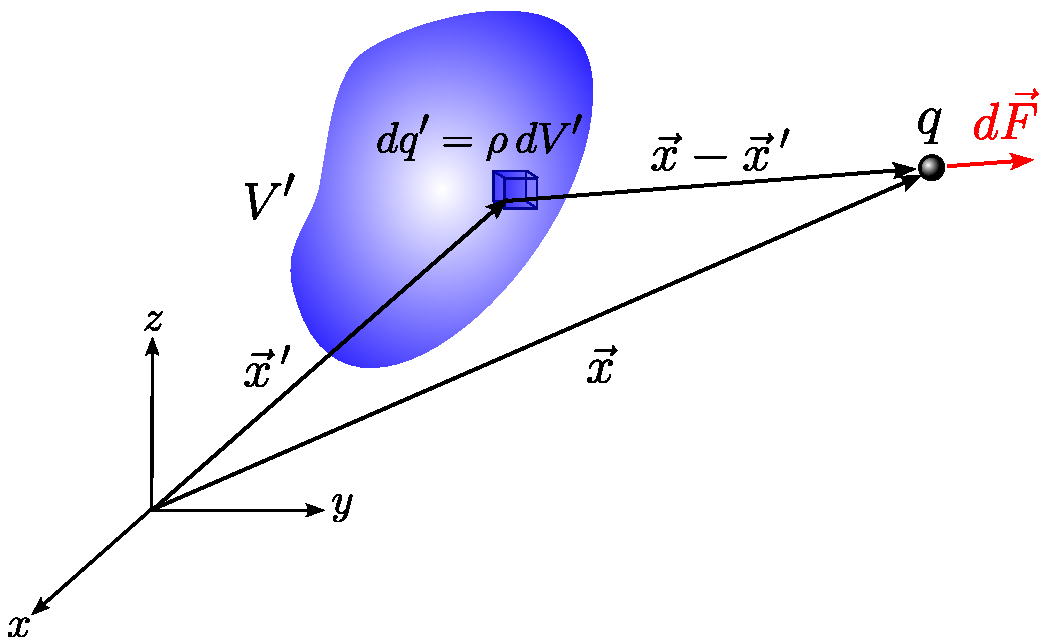
\includegraphics[scale = 0.6]{Figuras/Distribucion-Cargas-Fuerza.pdf}
    \caption{Distribución de carga.}
    \label{fig:Distribu-Carga}
\end{figure}

\begin{shaded}
   \begin{equation*}
d\vec{F} = \frac{1}{4\pi \varepsilon_0} \frac{q \,dq'}{|\vec{x} - \vec{x}\,'|^3} (\vec{x}- \vec{x}\,'),
\end{equation*} 
\end{shaded}

donde $\vec{x}$ es el vector posición de la carga $q$ (constante) y $\vec{x}\,'$ es el vector posición del elemento de carga $dq'$ (no constante).

Para el cálculo de la fuerza debemos integrar, pero necesitamos conocer la forma geométrica del cuerpo y la manera en que varía la \textbf{densidad de carga} en todos sus puntos.

En la práctica es conveniente describir la distribución de carga en función de \textit{densidades de carga}, pues la carga puede estar distribuida en una línea, superficie o volumen.

\begin{itemize}
\item[i)] \textbf{Densidad volumétrica de carga:}
\begin{equation*}
\rho = \frac{dq}{dV} ~ \left[\frac{C}{m^3} \right] \rightarrow dq' = \rho \, dV' ~\rightarrow~ d \vec{F} = k \frac{q \rho \,dV'}{|\vec{x} - \vec{x}\,'|^3} (\vec{x} - \vec{x}\,')
\end{equation*}

\item[ii)] \textbf{Densidad superficial de carga:}
\begin{equation*}
\sigma = \frac{dq}{dS} ~ \left[\frac{C}{m^2} \right] \rightarrow dq' = \sigma \, dS' \rightarrow d \vec{F} = k \frac{q \sigma \, dS'}{|\vec{x} - \vec{x}\,'|^3} (\vec{x} - \vec{x}\,')
\end{equation*}


\item[iii)] \textbf{Densidad lineal de carga:} 
\begin{equation*}
\lambda = \frac{dq}{dl} ~ \left[\frac{C}{m} \right] \rightarrow dq' = \lambda \, dl' \rightarrow d \vec{F} = k \frac{q \lambda \,dl'}{|\vec{x} - \vec{x}\,'|^3} (\vec{x} - \vec{x}\,')
\end{equation*}

\end{itemize}

En el caso de que, por ejemplo, $\rho$ sea uniforme:
\begin{equation*}
\rho = \frac{Q}{V},
\end{equation*}

donde $Q$ es la carga total y $V$ el volumen total de la distribución.

\textbf{Aclaración:} La forma en como se escribieron las densidades de carga puede resultar un poco confusa debido a que NO se trata de una derivada convencional, ésto es, $\rho$ no se obtiene al tomar $q$ como función del volumen y  derivar con respecto a $V$. Por ello, es mejor definir $\rho$ como la siguiente relación entre cantidades infinitesimales: $dq = \rho \,dV$ tal que al integrar se obtenga la carga total del sistema
$$Q = \iiint_V \rho \,dV.$$

Similarmente, para una distribución superficial y una lineal de carga:
$$Q = \iint_S \sigma\,dS \quad \text{o} \quad Q = \int_{L} \lambda \,dl.$$

\textbf{Observación:} Si las densidades de cargas $\lambda$, $\sigma$ y $\rho$ son constantes, se dice que se tiene una distribución de carga \textcolor{red}{uniforme}; pero si dependen de las coordenadas ($\rho(\vec{x}\,')$), obviamente se trata de una distribución de carga \textcolor{red}{no uniforme}.

El signo de la carga está incluido en ellas, por ejemplo,
\begin{equation*}
\lambda = -5 \times 10^{-6} ~ \left[ \frac{C}{m} \right].
\end{equation*}

\begin{ejemplo}
    Una carga eléctrica positiva $q$ está distribuida uniformente con densidad de carga $\lambda $ a lo largo de una línea de longitud $L$, que yace sobre el eje $y$ entre $y=-L$ e $y=L$. Encuentre la fuerza eléctrica que actúa sobre una carga $Q$ situada sobre el eje $x$ a una distancia $x$ del origen.

\begin{figure}[H]
    \centering
    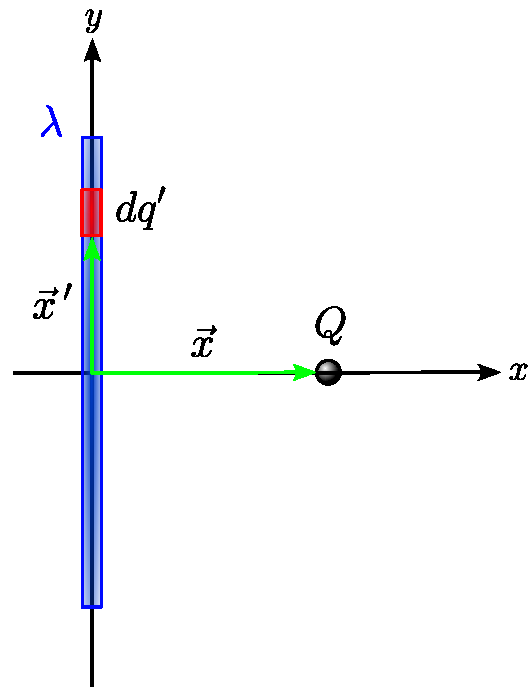
\includegraphics[scale = 0.6]{Figuras/Ej-Distribucion-Carga-1.pdf}
    \caption{Esquema de la situación física.}
    \label{fig:Ej-Distri-Carga-1}
\end{figure}

\textbf{Solución:} Usando coordenadas cartesianas, se tiene que
$$dq' = \lambda \,dy', \quad \Vec{x} = x \, \hat{\imath}, \quad \Vec{x}\,' = y' \,\hat{\jmath},$$

con $-L \leq y' \leq L$.

Por Coulomb, el diferencial de fuerza sobre $Q$ está dado por
\begin{align*}
    d\Vec{F} &= \frac{1}{4\pi \varepsilon_0}  \frac{Q \,dq'}{|\Vec{x} - \Vec{x}\,'|^3}(\Vec{x} - \Vec{x}\,') \\
    &= \frac{Q}{4\pi \varepsilon_0}  \frac{\lambda \,dy'}{|x \, \hat{\imath} - y' \,\hat{\jmath}|^3} (x \, \hat{\imath} - y' \,\hat{\jmath}) \\
    &= \frac{Q}{4\pi \varepsilon_0}  \frac{\lambda \,dy'}{(\sqrt{x^2 + y'\,^2})^3} (x \, \hat{\imath} - y' \,\hat{\jmath}).
\end{align*}

Integrando a ambos lados, la fuerza que actúa sobre $Q$ es
\begin{align*}
    \Vec{F} &= \frac{Q \lambda}{4\pi \varepsilon_0} \int_{-L}^L \frac{x \,\hat{\imath} - y' \,\hat{\jmath}}{(\sqrt{x^2 + y'\,^2})^3}  \,dy' \\
    &= \frac{Q \lambda}{4\pi \varepsilon_0} \left(x \int_{-L}^L \frac{1}{(\sqrt{x^2 + y'\,^2})^3} \,dy' \hat{\imath} + \int_{-L}^{L} \frac{y'}{(\sqrt{x^2+y'\,^2})^3} \,dy' \hat{\jmath} \right).  
\end{align*}

Usando las integrales del apéndice \ref{Integrales-Utiles}, en específico,

\begin{equation*}
\int \frac{1}{(\sqrt{x^2+y'\,^2})^3} \,dy' = \frac{y'}{x^2 \sqrt{x^2+y'\,^2}} + C \quad \text{y} \quad \int \frac{y'}{(\sqrt{x^2+y'\,^2})^3} \,dy' = - \frac{1}{\sqrt{x^2+y'\,^2}} +C,
\end{equation*}

tenemos que 
\begin{align*}
    \Vec{F} &= \frac{Q \lambda}{4\pi \varepsilon_0} \left[ x \frac{y'}{x^2 \sqrt{x^2+y'\,^2}} \hat{\imath} - \frac{1}{\sqrt{x^2+y'\,^2}} \hat{\jmath} \right]_{-L}^{L} \\
    &= \frac{Q \lambda}{4\pi \varepsilon_0} \frac{2L}{x \sqrt{x^2+L^2}} \hat{\imath}.
\end{align*}
\end{ejemplo}

\begin{ejemplo}
    Considere una distribución de carga lineal con forma de semi-circunferencia de radio $R$ y densidad de carga $\lambda$. Determine y calcule la fuerza que esta distribución ejerce sobre una carga puntual $q_0$ ubicada en el centro de curvatura.

\begin{figure}[H]
    \centering
    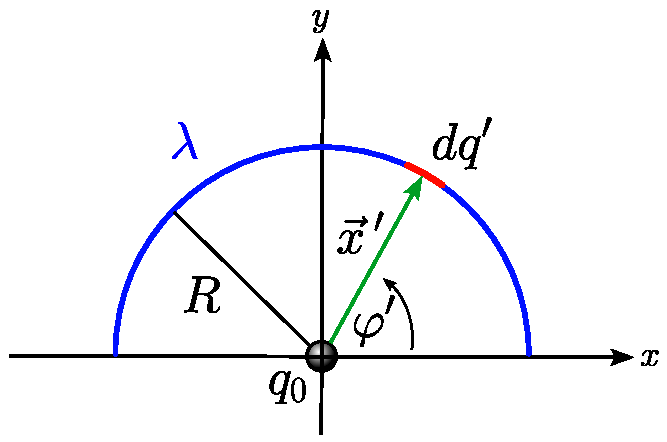
\includegraphics[scale = 0.6]{Figuras/Ej-Distribucion-Carga-2.pdf}
    \caption{Esquema de la situación física.}
    \label{fig:Ej-Distri-Carga-2}
\end{figure}


\textbf{Solución:} Usando coordenadas polares (cilíndricas con $z = 0$), se tiene que
$$dq' = \lambda R \,d\varphi', \quad \Vec{x} = \Vec{0}, \quad \Vec{x}\,' = R \,\hat{\rho} = R (\cos \varphi ' \,\hat{\imath} + \sin \varphi ' \,\hat{\jmath}),$$

con $0 \leq \varphi ' \leq \pi$.

Por Coulomb, el diferencial de fuerza sobre $q_0$ está dado por
\begin{align*}
    d\Vec{F} &= \frac{1}{4\pi \varepsilon_0}  \frac{q_0 \,dq'}{|\Vec{x} - \Vec{x}\,'|^3}(\Vec{x} - \Vec{x}\,) \\
    &= \frac{q_0}{4\pi \varepsilon_0}  \frac{\lambda R \,d\varphi'}{|\Vec{0} - R \hat{\rho}|^3} (\Vec{0} - R \,\hat{\rho}) \\
    &=- \frac{q_0}{4\pi \varepsilon_0}  \frac{\lambda R^2 \,d \varphi'}{R^3} \,\hat{\rho} \\
    &= - \frac{q_0}{4\pi \varepsilon_0}  \frac{\lambda \,d \varphi'}{R} \,\hat{\rho}.
\end{align*}

Integrando a ambos lados, la fuerza que actúa sobre $q_0$ es
\begin{align*}
\Vec{F} &=   - \frac{1}{4\pi \varepsilon_0} \frac{q_0 \lambda}{R}  \int_0^{2\pi}  \,\hat{\rho} \,d\varphi' \\
&= - \frac{1}{4\pi \varepsilon_0} \frac{q_0 \lambda}{R}  \int_0^{2\pi} \cos \varphi ' \,\hat{\imath} + \sin \varphi  '\,\hat{\jmath} \,d\varphi' \\
&= - \frac{1}{4\pi \varepsilon_0} \frac{q_0 \lambda}{R}  \left[\sin \varphi' \, \hat{\imath} - \cos \varphi\,' \,\hat{\jmath} \right]_0^{\pi} \\
&= - \frac{1}{2\pi \varepsilon_0} \frac{q_0 \lambda}{R} \, \hat{\jmath}.
\end{align*}
\end{ejemplo}

\textbf{Observación:} Note que en el primer ejemplo los vectores unitarios salieron de la integral a excepción del segundo ejemplo. Ésto es debido a que los vectores unitarios cartesianos son constantes y los cilíndricos no lo son, por ejemplo, $\hat{\rho}$ es una función de $\varphi$.

\begin{ejemplo}
    Determine la fuerza que una esfera de radio $R$, carga $Q$ y densidad de carga $\rho = cte$, ejerce sobre una carga puntual $q_0$ colocada afuera de ella.
    
\begin{figure}[H]
    \centering
    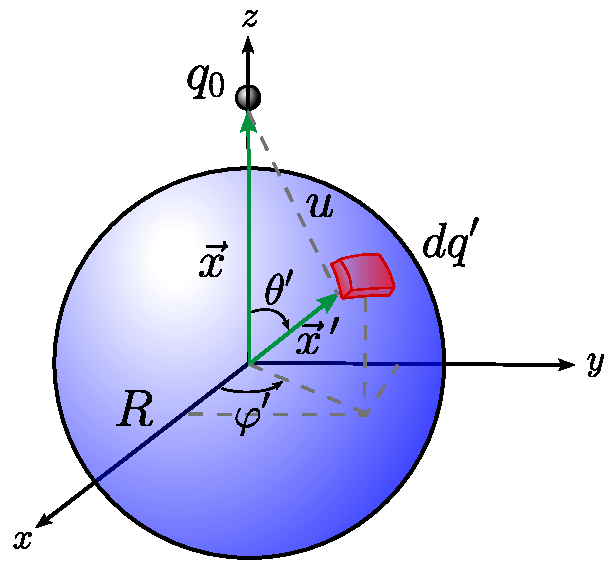
\includegraphics[scale = 0.65]{Figuras/Ej-Distribucion-Carga-3.pdf}
    \caption{Esquema de la situación física.}
    \label{fig:Ej-Distri-Carga-3}
\end{figure}

\textbf{Solución:} Consideremos una esfera maciza cargada uniformemente de radio $R$. Si nos movemos en una circunferencia de radio $r >R$ con el mismo centro que la esfera, observaremos la misma distribución y la fuerza electrostática tendrá la misma intensidad. Por lo tanto, situaremos nuestro sistema de referencia en el centro de ella y sin perder generalidad calcularemos la fuerza que ejerce la esfera sobre una carga puntual $q_0$ ubicada en el eje $z$, ver figura \ref{fig:Ej-Distri-Carga-3}.

Usando coordenadas esféricas, se tiene que
\begin{align*}
    dq' &= \rho \, dV' = \rho r'\,^2 \sin \theta' \,d \varphi' \,d\theta' \,dr', \\
    \Vec{x} \,' &= r' \,\hat{r} = r' (\cos \varphi ' \sin \theta' \,\hat{\imath} + \sin \varphi' \sin \theta' \,\hat{\jmath} + \cos \theta' \,\hat{k}),\\
    \Vec{x} &= z \,\hat{k},
\end{align*}

con $0 \leq r' \leq R$, $0 \leq \theta' \leq \pi$, $0 \leq \varphi' \leq 2\pi$ y $z\geq R$.

Por Coulomb, el diferencial de fuerza sobre $q_0$ está dado por
\begin{align*}
    d\Vec{F}&= \frac{1}{4\pi\varepsilon_0} \frac{q_0 \,dq'}{|\Vec{x} - \Vec{x}\,'|^3} (\Vec{x} - \Vec{x}\,') \\
    &= \frac{q_0 \rho}{4\pi \varepsilon_0} \frac{r'\,^2 \sin \theta' \,d \varphi' \,d\theta' \,dr' }{\left(\sqrt{z^2 + r'\,^2 - 2zr' \cos \theta'} \right)^3} (z\,\hat{k} - r' \,\hat{r}).
\end{align*}

Integrando a ambos lados, la fuerza que actúa sobre $q_0$ es
\begin{align*}
    \Vec{F} &= \frac{q_0 \rho}{4\pi \varepsilon_0} \int_0^R \int_0^{\pi} \int_0^{2\pi} \frac{r'\,^2 \sin \theta'  }{\left(\sqrt{z^2 + r'\,^2 - 2zr' \cos \theta'} \right)^3} (z\,\hat{k} - r' \,\hat{r}) \,d \varphi' \,d\theta' \,dr' \\
    &= \frac{q_0 \rho}{4\pi \varepsilon_0} \int_0^R \int_0^{\pi}  \frac{r'\,^2 \sin \theta'  }{\left(\sqrt{z^2 + r'\,^2 - 2zr' \cos \theta'} \right)^3} \left(\int_0^{2\pi} z\,\hat{k} - r' \,\hat{r} \,d \varphi' \right)\,d\theta' \,dr'.
\end{align*}

Resolvamos,
\begin{align*}
    \int_0^{2\pi} z \, \hat{k} - r' \,\hat{r}  \,d\varphi' &= \int_0^{2\pi} z \,\hat{k} - r'(\cos\varphi' \sin\theta' \, \hat{\imath} + \sin\varphi' \sin\theta' \, \hat{\jmath} + \cos\theta' \, \hat{k}) \,d\varphi' \\
    &= 2\pi (z-r'\cos\theta') \, \hat{k}.
\end{align*}

Luego,
$$\vec{F} =  \frac{ q_0 \rho}{2 \varepsilon_0} \, \hat{k} \int_0^R \int_0^{\pi} \frac{r'\,^2 \sin \theta' (z-r' \cos \theta')}{\left( \sqrt{z^2 + r'\,^2 -2zr' \cos \theta'} \right)^3} \,d\theta' \,dr'.$$

Sea $u > 0$ tal que
\begin{align*}
     u = \sqrt{z^2 + r'\,^2 - 2zr' \cos\theta'} & \Rightarrow  u^2 = z^2 + r'\,^2 - 2zr' \cos\theta' \\
     &\Rightarrow d(u^2) = \frac{d}{d \theta'} [z^2 + r'\,^2 - 2zr' \cos\theta' ] \,d\theta' \\
 & \Rightarrow  d(u^2) = 2zr' \sin \theta'\, d\theta' \\
 & \Rightarrow  u\,du = z r' \sin \theta'\, d\theta'.
\end{align*}

Usando la sustitución (altamente no trivial),
$$\cos \theta' = \frac{z^2 + r'\,^2 - u^2}{2zr'} \Rightarrow \sin \theta'\, d\theta' = \frac{u\,du}{zr'}.$$

Luego, los nuevos límites de integración son:
\begin{align*}
    \pi &\longrightarrow -2zr' = z^2+r'\,^2 -u^2 \Rightarrow  u = z + r', \\
    0 &\longrightarrow u^2 = (z-r')^2 ~\Leftrightarrow~ u = |z-r'| ~\Rightarrow ~ u = z - r'\quad (z \geq r',~ 0 \leq r' \leq R)
\end{align*}

Entonces, 
\begin{align*}
    \Vec{F} &= \frac{ q_0 \rho}{2 \varepsilon_0} \, \hat{k}  \int_0^R \left(\int_{z-r'}^{z+r'} \frac{r'\,^2}{u^3} \left(z- r' \frac{z^2 + r'\,^2 - u^2}{2z r'} \right)  \frac{u \,du}{zr'} \right) \,dr' \\
    &= \frac{ q_0 \rho}{2 \varepsilon_0} \, \hat{k}  \int_0^R \left(\int_{z-r'}^{z+r'} \frac{r'}{z u^2} \left( \frac{z^2 - r'\,^2 + u^2}{2z}  \right) \,du \right) \,dr' \\
    &= \frac{ q_0 \rho}{2 \varepsilon_0} \, \hat{k}  \int_0^R \frac{r'}{2z^2}\left(\int_{z-r'}^{z+r'}  \frac{z^2 - r'\,^2 + u^2}{u^2}  \,du \right) \,dr' \\
    &=  \frac{ q_0 \rho}{2 \varepsilon_0} \, \hat{k}  \int_0^R \frac{r'}{2z^2}\left[ u + \frac{r'\,^2 -z^2}{u} \right]_{z-r'}^{z+r'} \,dr' \\
    &= \frac{ q_0 \rho}{2 \varepsilon_0} \, \hat{k}  \int_0^R \frac{2 r'\,^2}{z^2} \,dr' \\
    &= \frac{ q_0 \rho}{2 \varepsilon_0} \, \hat{k}  \left[ \frac{2}{3z^2} r'\,^3 \right]_0^R \\
    &= \frac{q_0 \rho}{3 \varepsilon_0} \frac{R^3}{z^2} \hat{k} \\
    &= \frac{1}{4\pi \varepsilon_0} \frac{q_0 Q}{z^2} \,\hat{k},
\end{align*}

donde $\frac{4}{3} \pi R^3 \rho = Q$ con $Q$ la carga total de la esfera.
\end{ejemplo}

 \section{Campo eléctrico}

\textit{¿Cómo es posible que una carga eléctrica ejerza una fuerza sobre otra carga sin que no haya nada entremedio?}

En un principio se pensaba que las cargas ejercían una “acción a distancia”. La interpretación actual, desde \textit{Faraday }(1836), es que una carga eléctrica modifica el medio que la rodea y a la propiedad que adquiere se le llama \textbf{Campo Eléctrico} y es este campo el que actúa sobre las cargas que llegan o se encuentran en él.

Para averiguar si en un punto de un recinto existe un campo eléctrico, se coloca allí una carga de prueba $q$, supuesta positiva y pequeña con el fin de que no altere las propiedades del medio, y si dicha carga de prueba experimenta una fuerza es porque ahí existe un campo eléctrico.

Si se saca la carga de prueba, el campo sigue existiendo. Así, \textcolor{red}{el campo eléctrico es el intermediario entre las cargas que interactúan.}

Se define la \textbf{intensidad de campo eléctrico} $\vec{E}$ en un punto ($\vec{x}$) a la fuerza eléctrica en cada unidad de carga que experimenta una carga en ese punto. Se define operacionalmente como:
$$\boxed{\vec{E}(\vec{x}) := \lim_{q \to 0} \frac{\vec{F}}{q}}$$

Note que el proceso $\lim\limits_{q \to 0}$ es necesario dado que el uso de una carga $q$ de forma y magnitud arbitraria en general (mediante la interacción coulombiana) modificará la distribución de cargas original. Si la carga $q$ es cada vez más pequeña en extensión y magnitud, entonces ésta modificará cada vez menos la distribución de carga original.

Si se conoce el campo eléctrico (en el vacío), entonces la fuerza eléctrica que experimenta una carga puntual $q$ es
$$\boxed{\vec{F} = q \vec{E}(\vec{x})}$$

Supongamos que tenemos una carga $q'$ y una carga puntual $q$, por la ley de Coulomb, tenemos que
$$\vec{F} = \frac{1}{4\pi \varepsilon_0} \frac{q q'}{|\vec{x} - \vec{x}\,'|^3} (\vec{x} - \vec{x}\,').$$

Entonces, por la definición de campo eléctrico, podemos escribir
\begin{equation*}
\vec{E}(\vec{x}) = \lim_{q \to 0} \frac{\vec{F}}{q} = \frac{1}{4\pi \varepsilon_0} \frac{ q'}{|\vec{x} - \vec{x}\,'|^3} (\vec{x} - \vec{x}\,').
\end{equation*}

En general, si consideramos $q$ como un punto de campo $\vec{x}$. El \textbf{campo eléctrico} generado por $q'$ en $\vec{x}$, está dado por
\begin{shaded}
$$\vec{E}(\vec{x}) = \frac{1}{4 \pi \varepsilon_0} \frac{ q'}{|\vec{x} - \vec{x}\,'|^3} (\vec{x} - \vec{x}\,').$$
\end{shaded}

El \textbf{principio de superposición} también es aplicable al campo eléctrico. Dado un conjunto de cargas puntuales $q_1,q_2, q_3, \dots, q_n$, con vectores posición $\vec{x}_1, \vec{x}_2, \vec{x}_3, \dots , \vec{x}_n$, entonces el campo eléctrico $\vec{E}$ en un punto situado en $\vec{x}$ causado por las cargas, será
\begin{shaded}
$$\vec{E}(\vec{x}) = \frac{1}{4\pi\varepsilon_0} \sum_{i=1}^n q_i \frac{\vec{x} - \vec{x}_i}{|\vec{x} - \vec{x}_i|^3}.$$
\end{shaded}

\subsection{Campo eléctrico para distribuciones continuas}

En este caso, al igual que para la ley de Coulomb, el vector unitario, $(\vec{x} - \vec{x}\,')/|\vec{x} - \vec{x}\,'|$, tiene dirección variable, que llega al punto donde queremos calcular el campo eléctrico dado por el vector $\vec{x}$ desde el elemento de carga $dq'$.

\begin{figure}[H]
    \centering
    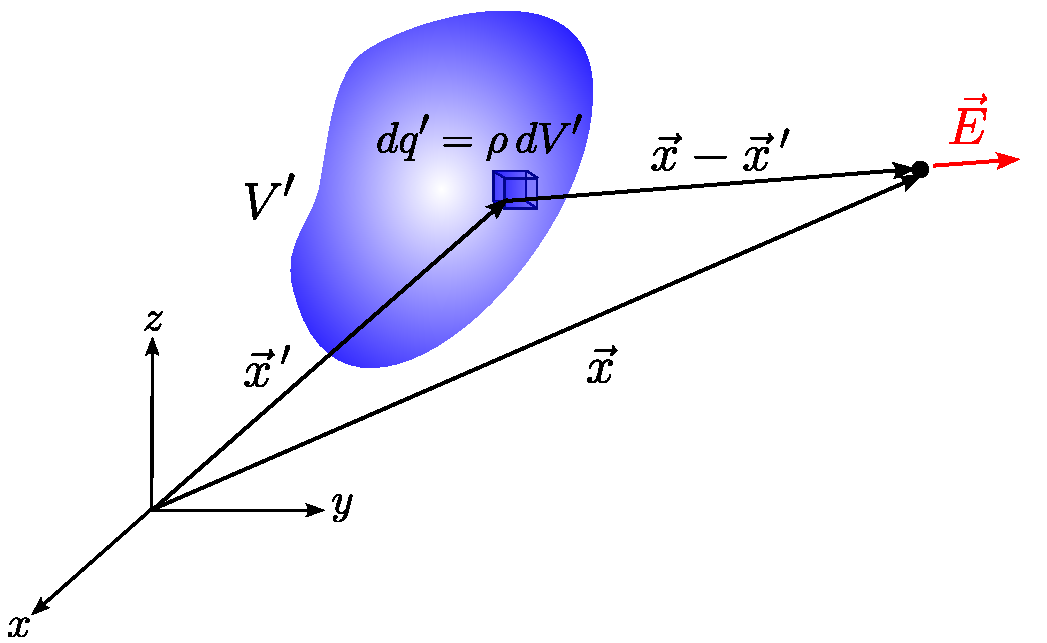
\includegraphics[scale = 0.6]{Figuras/Distribucion-Cargas-E.pdf}
    \caption{Distribución de carga.}
    \label{fig:Distribu-Carga2}
\end{figure}

\begin{equation*}
d\vec{E}(\vec{x}) = \frac{1}{4\pi \varepsilon_0} \frac{dq'}{|\vec{x} - \vec{x}\;'|^3} (\vec{x} - \vec{x}\;').
\end{equation*}

Si queremos calcular el campo eléctrico neto en $\vec{x}$, integramos ambos lados.
\begin{shaded}
    $$\vec{E}(\vec{x}) = \frac{1}{4\pi \varepsilon_0} \int \frac{dq'}{|\vec{x} - \vec{x}\;'|^3} (\vec{x} - \vec{x}\;').$$
\end{shaded}

En que, según sea el caso,
\begin{equation*}
dq = \rho \,dV = \sigma \,dS = \lambda \,dl.
\end{equation*}

\begin{ejemplo}
    Suponga que se tiene un alambre infinito sobre el eje $z$ y con densidad de carga uniforme igual a $\lambda$. Calcule el campo electrostático a una distancia $R$ del alambre.

\begin{figure}[H]
    \centering
    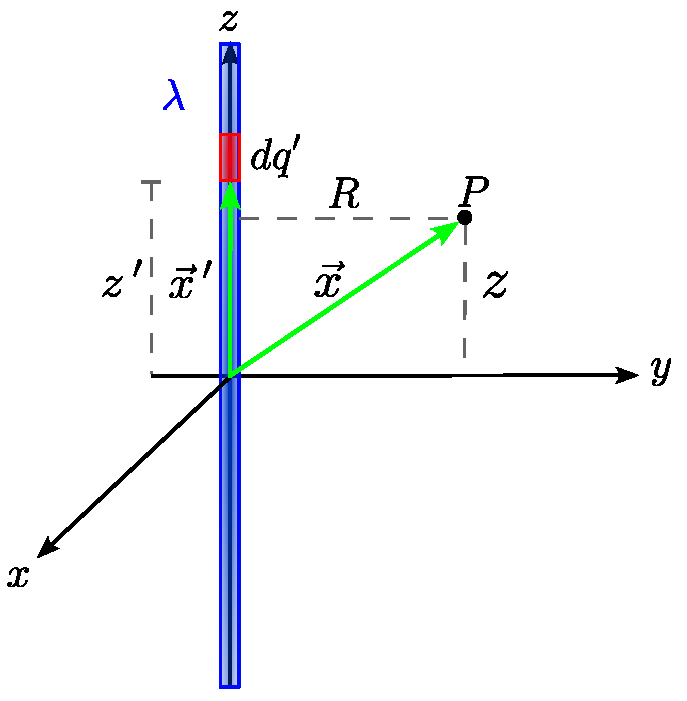
\includegraphics[scale = 0.6]{Figuras/Ej-E-Alambre-Infinito.pdf}
    \caption{Esquema de la situación física.}
    \label{fig:Ej-E-Alambre-Infinito}
\end{figure}

\textbf{Solución:} Considerando un punto $P$ cualquiera en el espacio, éste posee como vector posición:
$$\Vec{x} = R \,\hat{\rho} + z \, \hat{k}.$$

Usando coordenadas cilíndricas, se tiene que
$$dq' = \lambda \,dz', \quad \Vec{x}\,' = z' \,\hat{k},$$

con $- \infty < z' < \infty$.

Luego, el diferencial de campo eléctrico en el punto $P$ está dado por
\begin{align*}
    d \vec{E}(\vec{x}) &= \frac{1}{4\pi \varepsilon_0} \frac{dq'}{|\vec{x} - \vec{x}\,'|^3} (\vec{x} - \vec{x}\,')  \\
&= \frac{1}{4\pi \varepsilon_0} \frac{\lambda \,dz'}{|(R \,\hat{\rho} + z\, \hat{k}) - z' \,\hat{k}|^3} ((R \,\hat{\rho} + z \,\hat{k}) -z'\,\hat{k}) \\
&= \frac{\lambda}{4\pi \varepsilon_0} \frac{R \,\hat{\rho} + (z-z')\, \hat{k}}{(\sqrt{R^2 + (z-z')^2})^3} \,dz'.
\end{align*}

Integrando a ambos lados, el campo eléctrico es 
\begin{align*}
    \Vec{E}(\Vec{x}) &= \frac{\lambda}{4\pi \varepsilon_0} \int_{-\infty}^{\infty} \frac{R \,\hat{\rho} + (z-z')\, \hat{k}}{(\sqrt{R^2 + (z-z')^2})^3} \,dz' \\
    &= \frac{\lambda}{4\pi \varepsilon_0} \left[ \int_{-\infty}^{\infty} \frac{R}{(\sqrt{R^2 + (z-z')^2})^3} \,dz' \, \hat{\rho} + \int_{-\infty}^{\infty} \frac{z-z'}{(\sqrt{R^2 + (z-z')^2})^3} \,dz'\,\hat{k}\right].
\end{align*}

Si hacemos el cambio de variable $u = z - z' \Rightarrow du = - dz'$ en la segunda integral, tenemos que
$$\int_{-\infty}^{\infty} \frac{z-z'}{(\sqrt{R^2 + (z-z')^2})^3} \,dz' = \int_{\infty}^{-\infty} \frac{u}{(\sqrt{R^2 + u^2})^3} (- du) = \int_{-\infty}^{\infty} \frac{u}{(\sqrt{R^2 + u^2})^3} \,du.$$

El integrando es una función impar en $u$, ésto es, si
$$f(u) = \frac{u}{(\sqrt{R^2 + u^2})^3} \Rightarrow f(-u) = - \frac{u}{(\sqrt{R^2 + u^2})^3} = -f(u).$$

Entonces,  la integral desde $-\infty$ a $\infty$ en $u$, se anula. Así,
$$\Vec{E}(\Vec{x}) = \frac{\lambda}{4\pi \varepsilon_0}\int_{-\infty}^{\infty} \frac{R}{(\sqrt{R^2 + (z-z')^2})^3} \,dz' \, \hat{\rho} .$$

Resolviendo la integral indefinida:
$$\int \frac{R}{(\sqrt{R^2 + (z-z')^2})^3} \,dz' = - \frac{z-z'}{R\sqrt{R^2 + (z-z')^2}} + C .$$
 
Por lo tanto, 
\begin{align*}
    \vec{E}(\vec{x}) &= \frac{ \lambda}{4\pi \varepsilon_0} \left[ - \frac{z-z'}{R\sqrt{R^2 + (z-z')^2}} \right]_{-\infty}^{\infty} \hat{\rho} \\
&=  \frac{\lambda}{4\pi \varepsilon_0} \left[ - \frac{z-z'}{ R|z-z'|\sqrt{\frac{R^2}{(z-z')^2} + 1}} \right]_{-\infty}^{\infty} \hat{\rho} \\
&= \frac{\lambda}{4\pi \varepsilon_0} \left( \frac{1}{R} + \frac{1}{R} \right) \hat{\rho}  \\
&= \frac{\lambda}{2\pi \varepsilon_0 R} \,\hat{\rho}.
\end{align*}

\end{ejemplo}

\subsubsection{Campo eléctrico (radial):}

Ahora que se ha obtenido el resultado final, generalicemos para una distancia al eje $z$ arbitraria, lo cual se logra al sustituir $R \rightarrow \rho$.
$$\vec{E}(\Vec{x}) = \frac{\lambda}{2 \pi \varepsilon_0 \rho}\, \hat{\rho}.$$

En ella se observa que el campo eléctrico tiene simetría radial cilíndrica, ésto es, no depende de la coordenada $z$, el vector unitario tiene dirección perpendicular al alambre, y también se observa que la magnitud del campo es inversamente proporcional a la primera potencia de $\rho$.

\textbf{Observación:} Que sea inversamente proporcional a $\rho$ y no a $\rho^2$ significa que el campo de una línea o alambre es más intenso que si fuera el de una carga puntual. Además, este resultado es válido si el alambre es infinito o muy largo tal que no podemos ver los extremos, pues si es finito, al acercarnos a los extremos, el campo eléctrico tendrá una componente en $z$.

\begin{figure}[H]
\centering
\resizebox{12cm}{6cm}{%
\begin{tikzpicture}
[decoration={markings, 
	mark= at position 0.7 with {\arrow[]{latex}}}
] 

% Solve rotation issue
\path[] (-2,-3) rectangle (13.5,5);

% Rotate the illustration
\begin{scope}[transform canvas={rotate=10}]

% Electric Field (arrows of back layer) 
% 3D version
   
   \foreach \j in {1.25,5.75,9.75}
{
\draw[xshift=\j cm] (0,0) ellipse(0.2 and 0.5);
    \begin{scope}[xshift=\j cm,tdplot_main_coords]

        \foreach \angle in {0,45,...,180}
{
\tdplotsetcoord{P2}{2}{\angle}{-40}
\tdplotsetcoord{P1}{0.5}{\angle}{-40}
\draw[thick,postaction={decorate}] (P1) -- (P2);

}
    \end{scope}
}



% Cylindrical shape
\draw [top color= OliveGreen,
			bottom color= OliveGreen,
			middle color=YellowGreen,
			opacity=0.92] (0,-0.5) -- ++(12,0) 
	arc(-90:90:0.2 and 0.5) -- ++(-12,0) 
	arc(90:-90:0.2 and 0.5)--cycle;

\draw[fill=cyan!10] (0,0) ellipse(0.2 and 0.5);



% Electric charge
\foreach \j in {1,3.5,7,11} 
{
	\node at (\j,0){$\textbf{+}$};
}

% Electric Field (arrows of front layer) 
% 3D version

\foreach \j in {1.25,5.75,9.75}
{
    \begin{scope}[xshift=\j cm,tdplot_main_coords]
        \foreach \angle in {180,225,...,360}
{
\tdplotsetcoord{P2}{2}{\angle}{-40}
\tdplotsetcoord{P1}{0.5}{\angle}{-40}
\draw[thick,postaction={decorate}] (P1) -- (P2);

}
    \end{scope}
}


\end{scope} % end scope of the illustration rotation

\end{tikzpicture}
}
\caption{Campo eléctrico de un alambre infinito. Recuperado de: \href{https://latexdraw.com/electric-field-of-line-charge-in-tikz/}{latexdraw.com}.}
\end{figure}

\begin{ejemplo}
     Calcule el campo electrostático en un punto arbitrario que no se encuentre en el plano generado por un plano infinito que posee una densidad de carga uniforme $\sigma$. 

\begin{figure}[H]
    \centering
    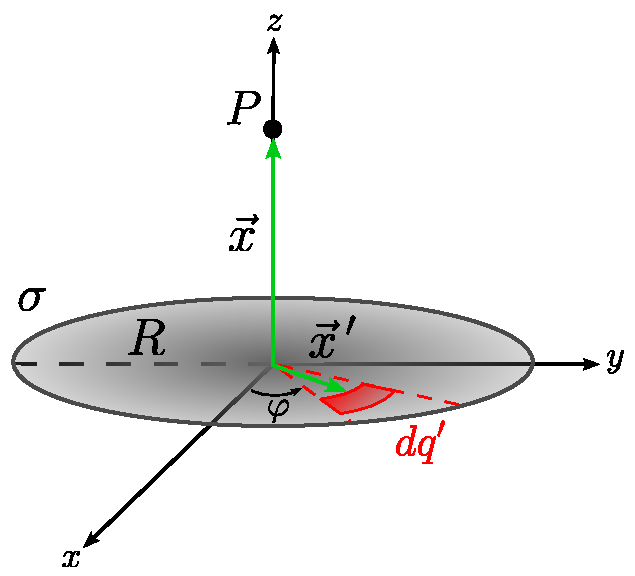
\includegraphics[scale = 0.65]{Figuras/Ej-E-Plano-Infinito.pdf}
    \caption{Esquema de la situación física.}
    \label{fig:Ej-E-Plano-Infinito}
\end{figure}

\textbf{Solución:} Si tenemos un plano infinito y tomamos un punto $P$ que no se encuentre en el plano. Podemos calcular el campo eléctrico en $P$ en el eje $z$, pues se puede tomar un vector normal al plano con dirección pasando por $P$, y un disco de centro en el origen y radio $R$ que se aplicará la condición $R \rightarrow \infty$ para tener el plano infinito, ver figura \ref{fig:Ej-E-Plano-Infinito}.

Usando coordenadas cilíndricas, se tiene que
$$dq' = \sigma \rho \, d\varphi' \,d\rho', \quad \Vec{x} = z \,\hat{k}, \quad \vec{x}\,' = \rho' \,\hat{\rho} = \rho' (\cos \varphi' \,\hat{\imath} + \sin \varphi' \, \hat{\jmath}),$$

con $0 \leq \rho' \leq R$, $0 \leq \varphi ' \leq 2\pi$.

Entonces, el diferencial de campo eléctrico en $\vec{x}$ es
\begin{align*}
    d\Vec{E}(\Vec{x}) &= \frac{1}{4\pi \varepsilon_0} \frac{dq'}{|\vec{x}  - \vec{x}\,'|^3} (\vec{x} - \vec{x}\,') \\
    &=  \frac{\sigma}{4\pi \varepsilon_0} \frac{z \,\hat{k} - \rho' \,\hat{\rho}}{\left( \sqrt{z^2 + \rho'\,^2} \right)^3}\, \rho' \,d\varphi\,' d\rho'.
\end{align*}

Integrando a ambos lados, el campo eléctrico está dado por
\begin{align*}
    \Vec{E}(\Vec{x}) &= \frac{\sigma}{4\pi \varepsilon_0} \int_0^R \int_0^{2\pi} \frac{z \,\hat{k} - \rho' \,\hat{\rho}}{\left( \sqrt{z^2 + \rho'\,^2} \right)^3} \,\rho' \,d\varphi\,' d\rho' \\
    &= \frac{\sigma}{4\pi \varepsilon_0} \int_0^R \frac{\rho'}{\left( \sqrt{z^2 + \rho'\,^2} \right)^3} \left(\int_0^{2\pi} (z \,\hat{k} - \rho' \,\hat{\rho} ) \,d\varphi\,' \right)d\rho' \\
    &= \frac{\sigma}{4\pi \varepsilon_0} \int_0^R \frac{\rho'}{\left( \sqrt{z^2 + \rho'\,^2} \right)^3} \left(\int_0^{2\pi} z \,\hat{k} \,d\varphi' - \rho' \int_0^{2\pi} \hat{\rho}  \,d\varphi\,' \right)d\rho' .
\end{align*}


Como 
$$\int_0^{2\pi} \hat{\rho} \,d\varphi' = \int_0^{2\pi} (\cos \varphi' \, \hat{\imath} + \sin \varphi'\,\hat{\jmath}) \, d\varphi' = \Vec{0},$$

se tiene que 
\begin{align*}
    \Vec{E}(\Vec{x}) &= \frac{\sigma}{4\pi \varepsilon_0} \int_0^R \frac{\rho'}{\left( \sqrt{z^2 + \rho'\,^2} \right)^3} \left(\int_0^{2\pi} z \,\hat{k} \,d\varphi'\right)d\rho' \\
    &= \frac{\sigma}{4\pi \varepsilon_0} \int_0^R \frac{\rho'}{\left( \sqrt{z^2 + \rho'\,^2} \right)^3} \, 2\pi z \, \hat{k} d\rho' \\
    &= \frac{\sigma}{2 \varepsilon_0} z \,\hat{k} \int_0^R\frac{\rho'}{\left( \sqrt{z^2 + \rho'\,^2} \right)^3} \,d\rho'.
\end{align*}

Usando la integral \eqref{A-I3} del apéndice \ref{Integrales-Utiles}, se obtiene
\begin{align*}
    \Vec{E}(\Vec{x}) &= \frac{\sigma z}{2 \varepsilon_0}  \,\hat{k} \left[ - \frac{1}{\sqrt{z^2 + \rho'\,^2}}\right]_0^R \\
    &= \frac{\sigma z}{2 \varepsilon_0}  \left(\frac{1}{|z|} - \frac{1}{\sqrt{z^2 + R^2}} \right) \,\hat{k}.
\end{align*}

Finalmente, tomamos el límite cuando $R \to \infty$.
\begin{align*}
    \lim_{R \to \infty} \Vec{E}(\Vec{x}) &= \frac{\sigma z}{2 \varepsilon_0}  \lim_{R\to \infty} \left(\frac{1}{|z|} - \frac{1}{\sqrt{z^2 + R^2}}\right) \hat{k} \\
    &= \frac{\sigma z}{2 \varepsilon_0 |z|} \,\hat{k}.  .
\end{align*}

Por lo tanto, el campo eléctrico de un plano infinito, en cualquier punto del espacio, es
\begin{equation*}
\vec{E}(\vec{x}) = \left\{ \begin{array}{c}
\scaleto{\frac{\sigma}{2 \epsilon_0}}{20pt} \, \hat{k} ~~,~~ \mbox{si} ~z>0 \\ \\
-\scaleto{\frac{\sigma}{2 \epsilon_0} }{20pt}\, \hat{k} ~,~~\mbox{si}  ~z<0
\end{array} \right.
\end{equation*}
\end{ejemplo}

\begin{ejemplo}
    Considere un cascarón esférico de radio $R$ y con densidad de carga uniforme $\sigma$. Calcule la intensidad del campo electrostático en un punto al interior del cascarón.
    
\begin{figure}[H]
    \centering
    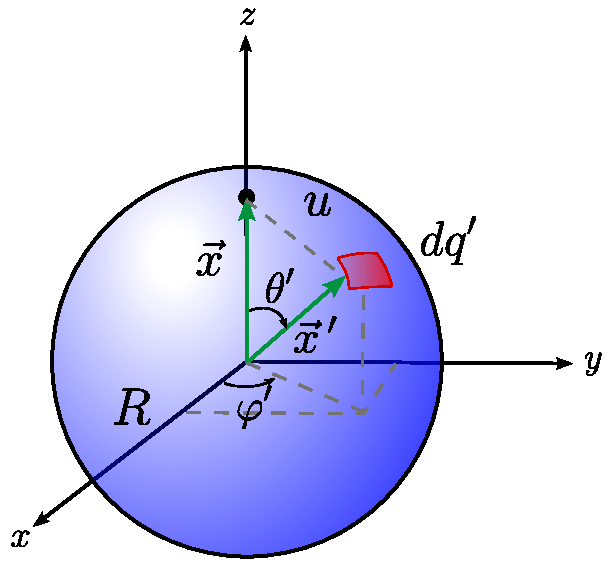
\includegraphics[scale = 0.65]{Figuras/Ej-E-Cascaron-Esferico.pdf}
    \caption{Esquema de la situación física.}
    \label{fig:Ej-E-Cascaron}
\end{figure}

\textbf{Solución:} Consideremos un cascarón esférico cargado uniformemente de radio $R$. Si nos movemos en una circunferencia de radio $r < R$ con el mismo centro que la esfera, observaremos la misma distribución y el campo eléctrico tendrá la misma intensidad. Por lo tanto, situaremos nuestro sistema de referencia en el centro de ella y sin perder generalidad calcularemos el campo electrostático en un punto situado en el eje $z$, ver figura \ref{fig:Ej-E-Cascaron}.

Usando coordenadas esféricas, se tiene que
\begin{align*}
    dq' &= \sigma R^2 \sin \theta\,d\theta'\,d\varphi', \\
    \Vec{x} &= z \, \hat{k}, \\
    \Vec{x}\,' &= R \,\hat{r} = R (\sin \theta' \cos \varphi' \, \hat{\imath} + \sin \theta' \sin\varphi' \,\hat{\jmath} + \cos \theta' \,\hat{k}),
\end{align*}

con $0 \leq \theta' \leq \pi$, $0 \leq \varphi' \leq 2\pi$ y $0 < z < R$.

Entonces, el diferencial de campo eléctrico en $\vec{x}$ es
\begin{align*}
    d\Vec{E}(\Vec{x}) &= \frac{1}{4\pi \varepsilon_0} \frac{dq'}{|\Vec{x} - \Vec{x}\,'|^3} (\Vec{x} - \Vec{x}\,') \\
    &= \frac{\sigma}{4\pi \varepsilon_0} \frac{R^2 \sin \theta'\, d\theta' \,d\varphi'}{|z\,\hat{k} - R\,\hat{r}|^3} (z\,\hat{k} - R \hat{r}) \\
    &= \frac{\sigma}{4\pi \varepsilon_0} \frac{z\,\hat{k} - R \hat{r}}{\left( \sqrt{z^2 + R^2 - 2zR \cos \theta'}\right)^3} R^2 \sin \theta' \,d\theta'\,d\varphi'.
\end{align*}

Integrando a ambos lados, el campo eléctrico está dado por
\begin{align*}
    \Vec{E}(\Vec{x}) &= \frac{\sigma R^2}{4\pi \varepsilon_0} \int_0^{\pi} \int_0^{2\pi} \frac{\sin \theta' (z\,\hat{k} - R \hat{r})}{\left( \sqrt{z^2 + R^2 - 2zR \cos \theta'}\right)^3} \,d\varphi'\,d\theta' \\
    &= \frac{\sigma R^2}{4\pi \varepsilon_0} \int_0^{\pi} \frac{\sin \theta'}{\left( \sqrt{z^2 + R^2 - 2zR \cos \theta'}\right)^3} \left( \int_0^{2\pi} (z\,\hat{k} - R \, \hat{r}) \,d\varphi'  \right)  \,d\theta'. 
\end{align*}

Resolvamos,
\begin{align*}
  \int_0^{2\pi} (z\,\hat{k} - R \, \hat{r}) \,d\varphi' &=    \int_0^{2\pi} (z\,\hat{k} - R (\sin \theta' \cos \varphi' \, \hat{\imath} + \sin \theta' \sin\varphi' \,\hat{\jmath} + \cos \theta' \,\hat{k})) \,d\varphi' \\
  &= 2\pi (z - R\cos\theta') \,\hat{k}.
\end{align*}

Luego,
$$\Vec{E}(\Vec{x}) = \frac{\sigma R^2}{2 \varepsilon_0} \,\hat{k} \int_0^{\pi} \frac{\sin \theta'(z-R \cos \theta')}{\left( \sqrt{z^2 + R^2 - 2zR \cos \theta'}\right)^3}   \,d\theta'.$$

Sea $u > 0$ tal que
\begin{align*}
     u = \sqrt{z^2 + R^2 - 2zR \cos\theta'} & \Rightarrow  u^2 = z^2 + R^2 - 2zR \cos\theta' \\
     &\Rightarrow d(u^2) = \frac{d}{d \theta'} [z^2 + R^2 - 2zR \cos\theta' ] \,d\theta' \\
 & \Rightarrow  d(u^2) = 2zR \sin \theta'\, d\theta' \\
 & \Rightarrow  u\,du = z R \sin \theta'\, d\theta'.
\end{align*}

Usando la sustitución (altamente no trivial),
$$\cos \theta' = \frac{z^2 + R^2 - u^2}{2zR} \Rightarrow \sin \theta'\, d\theta' = \frac{u\,du}{zR}.$$

Luego, los nuevos límites de integración son:
\begin{align*}
    \pi &\longrightarrow -2zR = z^2+R^2 -u^2 \Rightarrow  u = z + R, \\
    0 &\longrightarrow u^2 = (z-R)^2 ~\Leftrightarrow~ u = |z-R| ~\Rightarrow ~ u =  R - z \quad (0 < z < R).
\end{align*}

Entonces, 
\begin{align*}
    \Vec{E}(\Vec{x}) &= \frac{\sigma R^2}{2 \varepsilon_0} \,\hat{k} \int_{R-z}^{R+z} \frac{1}{u^3} \left( z - \frac{z^2+R^2-u^2}{2z}\right) \frac{u}{zR} \,du \\
    &= \frac{\sigma R^2}{2 \varepsilon_0} \,\hat{k} \int_{R-z}^{R+z} \frac{z^2 - R^2 + u^2}{2z} \cdot \frac{1}{u^2 z R} \,du \\
    &= \frac{\sigma R}{4 \varepsilon_0 z^2} \,\hat{k} \int_{R-z}^{R+z} \frac{z^2 - R^2 + u^2}{u^2}  \,du \\
    &= \frac{\sigma R}{4 \varepsilon_0 z^2} \,\hat{k} \left[u + \frac{R^2 - z^2}{u} \right]_{R-z}^{R+z} \\
    &= \frac{\sigma R}{4 \varepsilon_0 z^2} \,\hat{k} \left[2z + \frac{R^2-z^2}{R+z} - \frac{R^2-z^2}{R-z} \right] \\
    &= \Vec{0}.
\end{align*}

Para $z = 0$ (el origen) queda de ejercicio probar que también $\vec{E}(\vec{0}) = \vec{0}$.
\end{ejemplo}
 
\section{Líneas de campo eléctrico}

Las \textbf{líneas de campo eléctrico} son líneas que intentan representarlo. Convenimos en dibujarlas en la dirección y sentido del campo eléctrico, de tal manera que el campo resulta \underline{tangente} a estas líneas. En un región en que el campo es continuo no se puede dibujar todas las líneas y es necesario espaciarlas. Estas líneas no se cortan ya que el campo es único.


\begin{itemize}
\item[a)] Para una carga puntual: 

\begin{figure}[H]
        \centering
        \subfigure[]{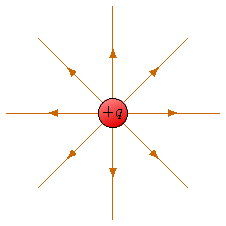
\includegraphics[width=0.36\textwidth]{Figuras/Campo-E-Carga+.pdf}} \hspace{1cm}
        \subfigure[]{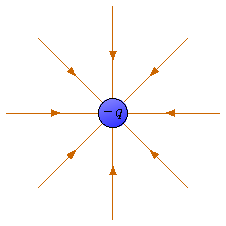
\includegraphics[width=0.36\textwidth]{Figuras/Campo-E-Carga-.pdf}} 
        \caption{Campo eléctrico de cargas puntuales positivas (a) y negativas (b). Recuperado de: \href{https://tikz.net/electric_fieldlines1/}{tikz.net}. }
        \label{fig:Campo-Cargas-Puntuales-1}
    \end{figure}

\item[b)] Para dos cargas puntuales de igual valor:

\begin{figure}[H]
        \centering
        \subfigure[]{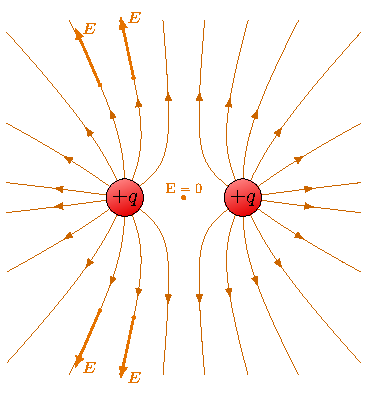
\includegraphics[width=0.36\textwidth]{Figuras/Campo-E-CargasIguales.pdf}} \hspace{1cm}
        \subfigure[]{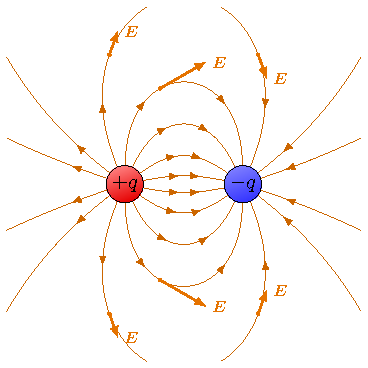
\includegraphics[width=0.36\textwidth]{Figuras/Campo-E-CargasOpuestas-.pdf}} 
        \caption{Campo eléctrico de dos cargas puntuales positivas (a) y opuestas (b). Recuperado de: \href{https://tikz.net/electric_fieldlines2/}{tikz.net}. }
        \label{fig:Campo-Cargas-Puntuales-2}
    \end{figure}

\item[c)] Para dos cargas puntuales de diferentes valores:

\begin{figure}[H]
        \centering
        \subfigure[]{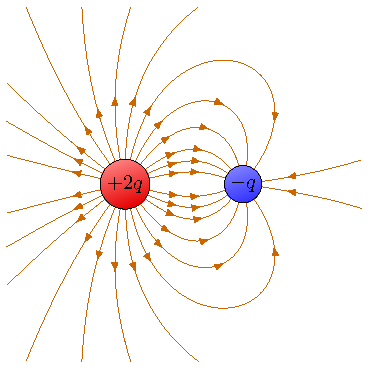
\includegraphics[width=0.36\textwidth]{Figuras/Campo-E-Cargas-MagDistintas-1.pdf}} \hspace{1cm}
        \subfigure[]{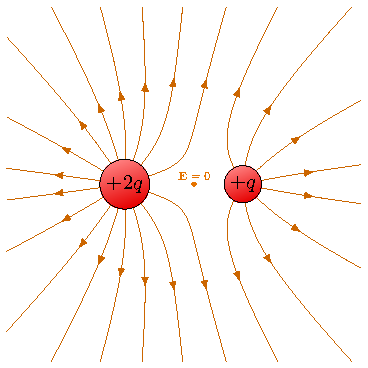
\includegraphics[width=0.36\textwidth]{Figuras/Campo-E-Cargas-MagDistintas-2.pdf}} 
        \caption{Campo eléctrico de cargas puntuales opuestas con distintos valores (a) y positivas con distintos valores (b). Recuperado de: \href{https://tikz.net/electric_fieldlines2/}{tikz.net}. }
        \label{fig:Campo-Cargas-Puntuales-3}
\end{figure}

\end{itemize}

\section{Flujo eléctrico}

Consideremos un campo vectorial que representa  al campo eléctrico generado por cargas en reposo. De ésta manera, el \textbf{flujo de campo eléctrico} queda definido por:
\begin{shaded}
    $$\Phi_E = \iint_S \Vec{E} \cdot d\Vec{S}.$$
\end{shaded}

Esta cantidad matemática mide el número de líneas que pasan a través de una superficie.

Las unidades de medida se desprenden de la definición: $[\Phi] = [\frac{N}{C} \,m^2]$.

Hay que notar que la superficie puede ser abierta o cerrada. En el caso de una \textit{superficie cerrada} el flujo se denota:
\begin{shaded}
    $$\Phi_E = \oiint_S \Vec{E} \cdot d\Vec{S}.$$
\end{shaded}

\textbf{Observación:} Si dentro de la superficie cerrada no hay ninguna carga, el número de líneas que entran en la superficie es igual al número de líneas que salen de ella. De este modo, el flujo neto será cero. 

Lo anterior se puede ver en el siguiente ejemplo.

\begin{ejemplo}
    Dado un campo eléctrico uniforme, calcule el flujo eléctrico a través de la superficie de un cubo y un cilindro tal como se indica en la figura \ref{fig:Flujo-E}.

\begin{figure}[H]
    \centering
    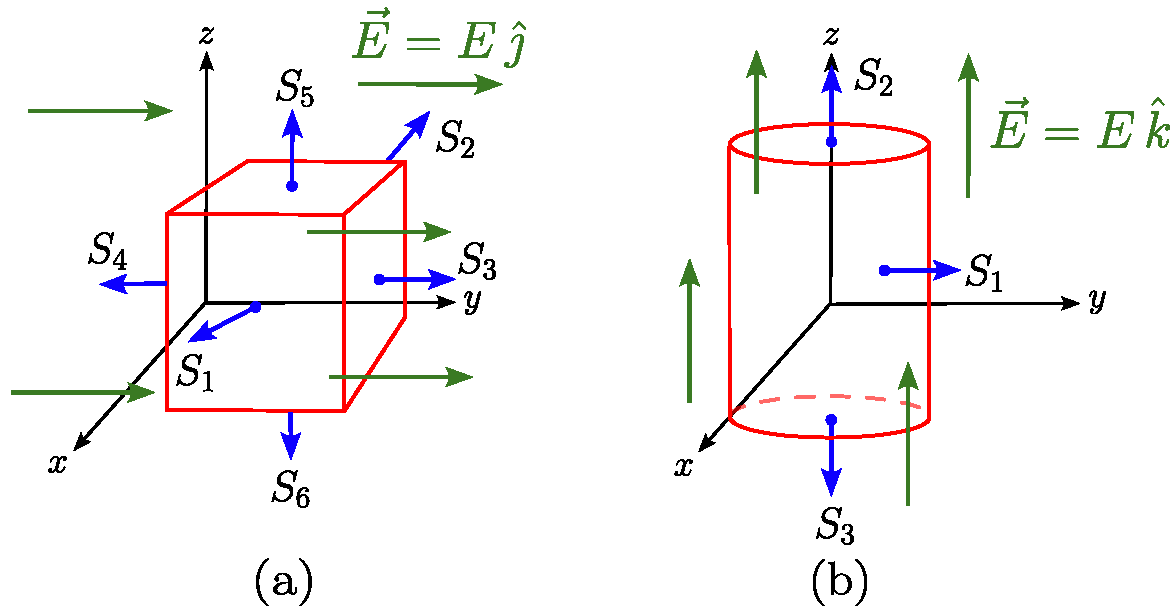
\includegraphics[scale = 0.6]{Figuras/Ej-Flujo-Electrico.pdf}
    \caption{Un cubo en presencia de un campo eléctrico uniforme en la dirección del eje $y$ (a) y un cilindro en presencia de un campo eléctrico uniforme en la dirección del eje $z$.}
    \label{fig:Flujo-E}
\end{figure}

\textbf{Solución:} Para el caso del cubo.
\begin{align*}
    \Phi_E &= \oiint_S \vec{E} \cdot d\vec{S} \\
&= \iint_{S_1} \vec{E} \cdot d\vec{S}_1 +  \iint_{S_2}\vec{E} \cdot d\vec{S}_2 + \iint_{S_3}\vec{E} \cdot d\vec{S}_3 \\
&\quad + \iint_{S_4}\vec{E} \cdot d\vec{S}_4 + \iint_{S_5}\vec{E} \cdot d\vec{S}_5 + \iint_{S_6}\vec{E} \cdot d\vec{S}_6  \\
&= \iint_{S_1} (E \hat{\jmath})\cdot(dydz \hat{\imath}) +  \iint_{S_2} (E \hat{\jmath})\cdot(-dydz \hat{\imath}) + \iint_{S_3} (E \hat{\jmath})\cdot(dxdz \hat{\jmath}) \\
&\quad + \iint_{S_4} (E \hat{\jmath})\cdot(-dxdz \hat{\jmath}) + \iint_{S_5} (E \hat{\jmath})\cdot(dxdy \hat{k}) + \iint_{S_6} (E \hat{\jmath})\cdot(-dxdy \hat{k}) \\
&= E \iint_{S_3} dxdz - E \iint_{S_4} dxdz\\
&= 0.
\end{align*}

Para el caso del cilindro:
\begin{align*}
\Phi_E &= \oiint_S \vec{E} \cdot d\vec{S} \\
&= \iint_{S_1}\vec{E} \cdot d\vec{S}_1 +  \iint_{S_2}\vec{E} \cdot d\vec{S}_2 + \iint_{S_3}\vec{E} \cdot d\vec{S}_3 \\
&= \iint_{S_1} (E \hat{k})\cdot(\rho d\varphi dz \hat{\rho}) +  \iint_{S_2} (E \hat{k})\cdot( \rho d\rho d\varphi \hat{k}) + \iint_{S_3} (E \hat{k})\cdot( -\rho d\rho d\varphi \hat{k})  \\
&= E \iint_{S_2} \rho d\rho d\varphi  - E \iint_{S_3} \rho d\rho d\varphi  = 0.
\end{align*}


\end{ejemplo}

Un caso especial es cuando el campo eléctrico es uniforme, de tal manera que puede salir fuera de la integral.
$$\Phi_E = \iint_S \vec{E} \cdot d\vec{S} = \iint_S E dS \cos \theta = E \iint_S dS \cos \theta.$$

Es más, si el campo eléctrico es \underline{perpendicular} a la superficie ($\theta = 0$), se tiene
$$\Phi_E = E \iint_S dS \cos 0 = E \iint_S dS = E A,$$

donde $A$ es el área de la superficie.

\section{Ley de Gauss} \label{Ley-Gauss}

\subsection{Forma integral de la ley de Gauss}

La \textbf{ley de Gauss} es una consecuencia de la ley de Coulomb, \footnote{La demostración matemática de la ley de Gauss se escapa de los contenidos del curso.} pero está formulada de una manera tal que permite calcular fácilmente los campos eléctricos producidos por distribuciones de carga altamente simétricas. Por ejemplo: esferas aisladas, esferas concéntricas, cilindros aislados,
cilindros concéntricos, lineas rectas, planos aislados, planos paralelos, etc.

\textbf{Enunciado:} El flujo eléctrico total que atraviesa una superficie cerrada arbitraria es igual a la carga total encerrada dividida por la permitividad eléctrica del vacío $\varepsilon_0$.
\begin{shaded}
  $$\Phi_e = \oiint_S \vec{E} \cdot d\vec{S} = \frac{q_{encerrada}}{\varepsilon_0}. $$
\end{shaded}

La superficie $S$ se llama \textbf{superficie Gaussiana} y es una superficie imaginaria (matemática) que sirve para calcular la integral de superficie $\oint_S \vec{E} \cdot d\vec{S}$. La idea es escoger una superficie conveniente con el objetivo de facilitar el cálculo de la integral, para ello es crucial saber la forma del campo eléctrico.

Esta ley puede interpretarse, en electrostática, entendiendo el flujo como una medida del número de líneas de campo que atraviesan la superficie en cuestión. Para una carga puntual es evidente que este número es constante si la carga está contenida por la superficie y es nulo si está fuera. Además, al ser la densidad de líneas proporcionales a la magnitud de la carga, resulta que este flujo es proporcional a la carga, si está encerrada, o nulo, si no lo está.

\begin{figure}[H]
    \centering
    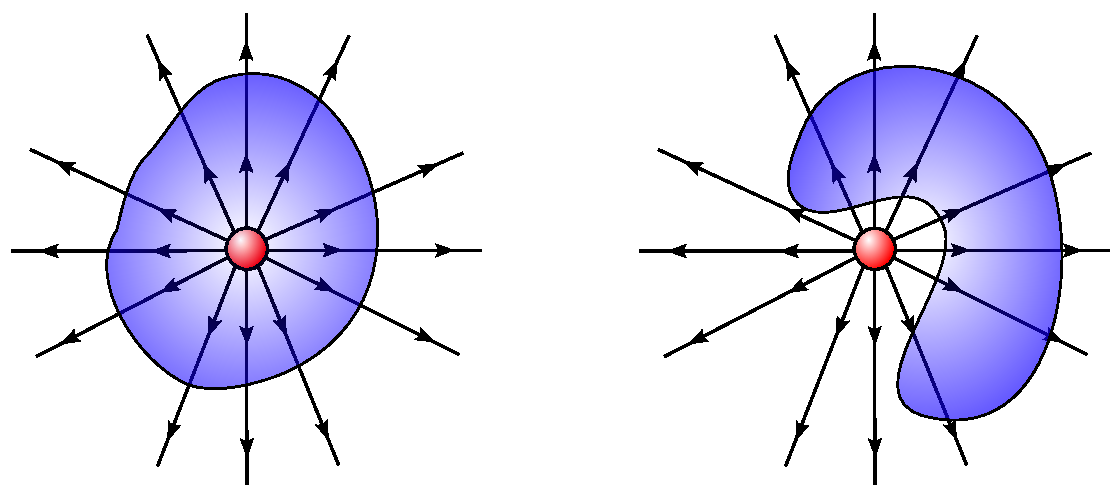
\includegraphics[scale = 0.6]{Figuras/LeyGauss.pdf}
    \caption{}
    \label{fig:Gauss-Law}
\end{figure}

Cuando tenemos una distribución de cargas, por el principio de superposición, sólo tendremos que considerar las cargas interiores, resultando la \textit{ley de Gauss}.

\begin{ejemplo}
     Una esfera de radio $R$ tiene una densidad volumétrica de carga $\rho = cte$. Determinar el campo eléctrico a) afuera de la esfera y b) adentro de ella.

\begin{figure}[H]
    \centering
    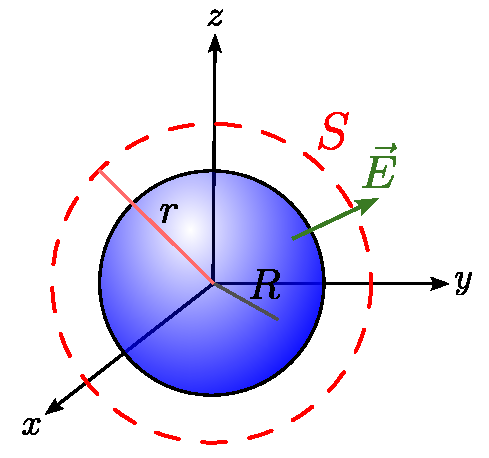
\includegraphics[scale = 0.7]{Figuras/Ej-Gauss-1.pdf}
    \caption{Superficie Gaussiana para la esfera de radio $R$ cargada uniformemente.}
    \label{fig:Ej-Gauss-1}
\end{figure}

\textbf{Solución:} El campo eléctrico de la esfera es radial, es decir, $\vec{E} = E \,\hat{r}$. Por ello, se aplicará la ley de Gauss utilizando como \textit{superficie Gaussiana} ($S$) el cascarón de una esfera centrada en el origen con radio $r$, donde el módulo del campo es constante a esa distancia.

\begin{itemize}
\item[a)] Para $r > R$, usando coordenadas esféricas, se tiene que

\begin{itemize}
\item $dq' = \rho r'\,^2 \sin \theta ' \,d\varphi'\, d\theta' dr'$ 

\item $d\vec{S} = r^2 \sin \theta \,d\varphi\, d\theta \, \hat{r}$ (diferencial de superficie de $S$).
\end{itemize}

Por la Ley de Gauss, tenemos que
\begingroup
\allowdisplaybreaks
\begin{align*}
    \oiint_S \vec{E} \cdot d\vec{S} &= \frac{q_{encerrada}}{\varepsilon_0} \\
    \int_0^{\pi} \int_0^{2\pi} (E \,\hat{r}) \cdot (r^2 \sin \theta\, d\varphi \,d\theta \,\hat{r}) &= \frac{1}{\varepsilon_0} \int_0^Q dq' \\
    \int_0^{\pi} \int_0^{2\pi} E   r^2 \sin \theta \, d\varphi \,d\theta &= \frac{1}{\varepsilon_0} \int_0^R\int_0^{\pi}\int_0^{2\pi} \rho r'\,^2  \sin \theta'\, d\varphi'\, d\theta'\, dr' \\
    2\pi E r^2 \int_0^{\pi} \sin \theta \,d\theta &= \frac{2\pi \rho}{\varepsilon_0} \int_0^R r'^2 \left( \int_0^\pi \sin \theta'\, d\theta' \right)  dr' \\ 
    4\pi r^2 E &= \frac{4}{3\varepsilon_0} \pi R^3 \rho \\
    E &= \frac{R^3 \rho}{3 \varepsilon_0 r^2}.
\end{align*}
\endgroup

Por lo tanto, 
$$\vec{E}(\vec{x}) = \frac{R^3 \rho}{3 \varepsilon_0 r^2} \,\hat{r} = \frac{1}{4\pi \varepsilon_0} \frac{Q}{r^2}\, \hat{r}, \quad r > R,$$ 

donde $Q$ es la carga total de la esfera.

\item[b)] Para $0 \leq r < R$, se tiene que la superficie Gaussiana encierra una esfera y un cascarón esférico, el campo que contribuye el cascarón es cero, por lo tanto el campo que a traviesa $S$ es radial (campo exterior de una esfera).

Usando coordenadas esféricas, se tiene que

\begin{itemize}
\item $dq' = \rho r'\,^2 \sin \theta'\, d\varphi'\, d\theta'\, dr'$ 

\item $d\vec{S} = r^2 \sin \theta\, d\varphi\, d\theta\, \hat{r}$ (diferencial de superficie de $S$).
\end{itemize}

Por la Ley de Gauss, tenemos que
\begin{align*}
    \oiint_S \vec{E} \cdot d\vec{S} &= \frac{q_{encerrada}}{\varepsilon_0} \\
    \int_0^{\pi} \int_0^{2\pi} (E \,\hat{r}) \cdot (r^2 \sin \theta\, d\varphi \,d\theta \,\hat{r}) &= \frac{1}{\varepsilon_0} \int_0^Q dq' \\
    \int_0^{\pi} \int_0^{2\pi} E   r^2 \sin \theta \, d\varphi \,d\theta &= \frac{1}{\varepsilon_0} \int_0^r\int_0^{\pi}\int_0^{2\pi} \rho r'\,^2  \sin \theta'\, d\varphi'\, d\theta'\, dr' \\
    2\pi E r^2 \int_0^{\pi} \sin \theta \,d\theta &= \frac{2\pi \rho}{\varepsilon_0} \int_0^r r'^2 \left( \int_0^\pi \sin \theta'\, d\theta' \right)  dr' \\ 
    4\pi r^2 E &= \frac{4}{3\varepsilon_0} \pi r^3 \rho \\
    E &= \frac{\rho r}{3 \varepsilon_0}.
\end{align*}

Por lo tanto, 
$$\vec{E}(\vec{x}) = \frac{ \rho r}{3 \epsilon_0} \, \hat{r} = \frac{1}{4\pi \varepsilon_0} \frac{Qr}{R^3} \,\hat{r}, \quad r < R .$$
\end{itemize}
\end{ejemplo} 


\begin{ejemplo}
     Encontrar el campo eléctrico a una distancia $R$ de un alambre infinito cuya densidad de carga lineal $\lambda = cte$.

\begin{figure}[H]
    \centering
    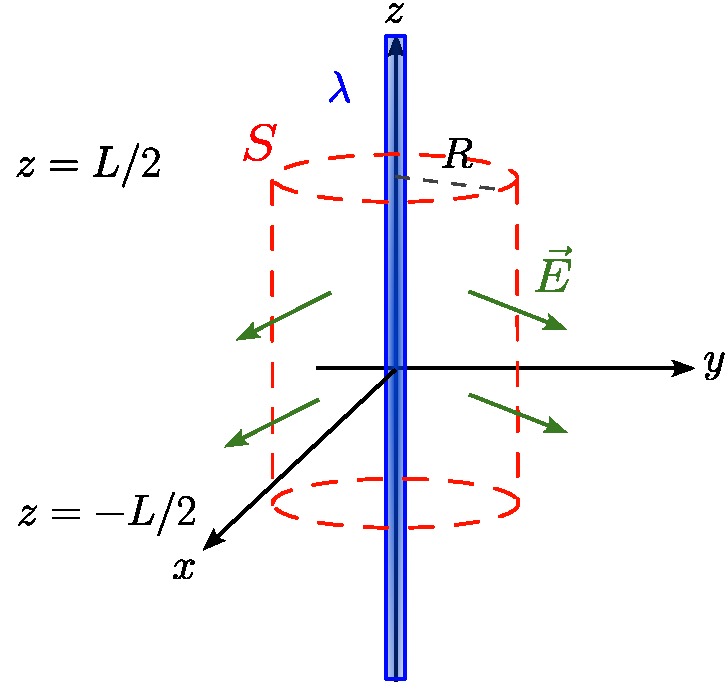
\includegraphics[scale = 0.65]{Figuras/Ej-Gauss-2.pdf}
    \caption{Superficie Gaussiana para un alambre infinito $R$ cargado uniformemente.}
    \label{fig:Ej-Gauss-2}
\end{figure}

\textbf{Solución:} El campo eléctrico del alambre infinito está en la dirección de $\hat{\rho}$, es decir, $\vec{E} = E \hat{\rho}$. Por ello, para aplicar la Ley de Gauss, se utilizará como \textit{superficie Gaussiana} un cilindro centrado en el origen de radio $R$, distancia donde queremos evaluar el campo, la cual el campo tiene módulo constante, y altura $L$ con la  tapa inferior en el plano $z = -L/2$ y la tapa superior en el plano $z = L/2$.

Usando coordenadas cilíndricas, se tiene que

\begin{itemize}
\item $dq = \lambda \,dz $ (diferencial de la carga encerrada),

\item $d\vec{S}_M = R \, d\varphi \,dz \hat{\rho} $ (elemento de superficie del manto).

\item $d\vec{S}_{TI} = - R \,d\varphi\, d\rho \,\hat{k}$ (elemento de superficie de la tapa inferior). 

\item $d\vec{S}_{TS} = R \,d\varphi\, d\rho \,\hat{k}$ (elemento de superficie de la tapa superior).
\end{itemize}

Calculemos
\begingroup
\allowdisplaybreaks
\begin{align*}
    \oiint_S \vec{E} \cdot d\vec{S} &= \iint_{S_{M}} \vec{E} \cdot d\vec{S}_M + \iint_{S_{TI}} \vec{E} \cdot d\vec{S}_{TI} + \iint_{S_{TS}} \vec{E} \cdot d\vec{S}_{TS} \\
    &= \int_{-L/2}^{L/2} \int_0^{2\pi} (E\,\hat{\rho}) \cdot (R\,d\varphi\, dz \,\hat{\rho}) + \cancelto{0}{\int_0^R \int_0^{2\pi} (E\,\hat{\rho})\cdot (- R \,d\varphi \,d\rho \,\hat{k} )} \\
    & \quad + \cancelto{0}{\int_0^R \int_0^{2\pi} (E\,\hat{\rho})\cdot (R \,d\varphi\, d\rho\, \hat{k})} \\
    &= \int_{-L/2}^{L/2} \int_0^{2\pi} E R \,d\varphi \,dz \\
    &= 2\pi L ER.
\end{align*}
\endgroup

Por la ley de Gauss, tenemos que
\begin{align*}
    \oiint_S \vec{E} \cdot d\vec{S} = \frac{q_{encerrada}}{\varepsilon_0} &\Rightarrow 2\pi L E R = \frac{1}{\varepsilon_0} \int_{-L/2}^{L/2} \lambda \,dz = \frac{\lambda L}{\varepsilon} \\
    &\Rightarrow E = \frac{\lambda}{2\pi \varepsilon_0 R}.
\end{align*}

Por lo tanto, generalizando ($R \to \rho$),
$$\Vec{E}(\Vec{x}) = \frac{\lambda}{2\pi \varepsilon_0 \rho} \,\hat{\rho}.$$

\end{ejemplo}

\begin{ejemplo}[Propuesto]
Determinar el campo electrostático  de un plano infinito en el plano $xy$. 

\textbf{Hint:} Tomar como superficie Gaussiana un cilindro centrado en el origen tal que el plano divida al cilindro en dos. 

\textbf{Solución:}  $\vec{E} = \frac{\sigma}{2\varepsilon_0} \,\hat{k}$ para $z > 0$ y $\vec{E} = - \frac{\sigma}{2 \varepsilon_0} \,\hat{k}$ para $z <0$.

\end{ejemplo}


\subsection{Forma diferencial de la ley de Gauss}

La ley de Gauss (para  la electrostática) está dada por
$$\oiint_S \vec{E} \cdot d\vec{S} = \frac{q}{\varepsilon_0}.$$

Para cargas distribuidas en un volumen, podemos escribir la carga por
$$q = \iiint_V \rho(\vec{x}) \,dV.$$

Luego, 
$$\oiint_S \vec{E} \cdot d\vec{S} = \frac{1}{\varepsilon_0} \iiint_V \rho(\vec{x}) \,dV.$$

Por el teorema de Gauss (de la divergencia), tenemos que
$$\oiint_S \vec{E} \cdot d\vec{S} = \iiint_V \vec{\nabla} \cdot \vec{E} \,dV$$ 

Por transitividad, 
\begin{equation*}
\iiint_V \frac{1}{\varepsilon_0} \rho (\vec{x}) d V =   \iiint_V \vec{\nabla} \cdot \vec{E} \,dV.
\end{equation*}

Así, hemos probado que \textcolor{red}{para todo volumen} $V$, se verifica
$$\iiint_V \left( \frac{1}{\varepsilon_0} \rho (\vec{x}) - \vec{\nabla} \cdot \vec{E}  \right) \, dV= 0.$$


Por lo tanto, se obtiene ecuación
\begin{shaded}
$$\vec{\nabla} \cdot \vec{E} = \frac{\rho(\vec{x})}{\varepsilon_0},$$    
\end{shaded}

conocida como la \textbf{primera ecuación de Maxwell}.


\chapter{Potencial electrostático}

\section{Introducción al potencial}

Un diferencial de  campo eléctrico, para una distribución continua de carga, está dado por:
$$d\vec{E}(\vec{x}) = \frac{1}{4\pi\varepsilon_0} \frac{dq'}{|\vec{x} - \vec{x}\;'|^2} \frac{(\vec{x} - \vec{x}\;')}{ |\vec{x} - \vec{x}\;'|}.$$

Integrando la ecuación y usando la relación $dq' = \rho(\vec{x}\;') \,dV' $ (suponiendo que se tiene una distribución volumétrica), tenemos que
$$\vec{E}(\Vec{x}) = \frac{1}{4\pi\varepsilon_0} \iiint_{V'} \rho(\vec{x}\,') \frac{(\vec{x} - \vec{x}\,')}{|\vec{x} - \vec{x}\,'|^3}\,dV'.$$

Pero,
\begin{equation}
 \frac{(\vec{x} - \vec{x}\,')}{|\vec{x} - \vec{x}\,'|^3} = - \vec{\nabla}_{\vec{x}} \left( \frac{1}{|\vec{x} - \vec{x}\,'|} \right).   \label{Identidad-Grad}
\end{equation}

\begin{demo}
En efecto, considerando que $ \vec{\nabla}_{\vec{x}} (\cdots) $ indica que el gradiente se calcula con respecto a las coordenadas de $ \vec{x} $ .

Sea $\vec{x} = (x,y,z)$ y $\vec{x}\,' = (x',y',z')$, se tiene
$$\frac{1}{|\vec{x} - \vec{x}\,'|} = \frac{1}{\sqrt{(x-x')^2 + (y-y')^2 + (z-z')^2}}.$$

Luego,
\begin{align*}
   \frac{\partial }{\partial x} \left[ \frac{1}{|\vec{x} - \vec{x}\,'|} \right] &= -\frac{1}{2 ((x-x')^2 + (y-y')^2 + (z-z')^2)^{3/2}} \cdot 2(x-x') \\
&= - \frac{(x-x')}{|\vec{x} - \vec{x}\,'|^3}, \\
\frac{\partial }{\partial y} \left[ \frac{1}{|\vec{x} - \vec{x}\,'|} \right] &= -\frac{1}{2 ((x-x')^2 + (y-y')^2 + (z-z')^2)^{3/2}} \cdot 2(y-y') \\ 
&= - \frac{(y-y')}{|\vec{x} - \vec{x}\,'|^3}, \\
\frac{\partial }{\partial z} \left[ \frac{1}{|\vec{x} - \vec{x}\,'|} \right] &= -\frac{1}{2 ((x-x')^2 + (y-y')^2 + (z-z')^2)^{3/2}} \cdot 2(z-z') \\ 
&= - \frac{(z-z')}{|\vec{x} - \vec{x}\,'|^3}. 
\end{align*}

Entonces,
$$ - \vec{\nabla}_{\vec{x}} \left( \frac{1}{|\vec{x} - \vec{x}\,'|} \right) = \frac{(\vec{x} - \vec{x}\,')}{|\vec{x} - \vec{x}\,'|^3} .$$
\end{demo}

Reemplazando en la expresión para el campo eléctrico.
$$\Vec{E}(\vec{x}) = - \frac{1}{4\pi \varepsilon_0} \iiint_{V'} \vec{\nabla}_{\vec{x}} \left( \frac{\rho(\vec{x}\,')}{|\vec{x} - \vec{x}\,'|} \right) dV'.$$

Como el gradiente depende de $\vec{x}$ y la integral es con respecto a las coordenadas de  $\vec{x}\,'$, podemos intercambiar el orden de estos.
\begin{equation}
\vec{E}(\Vec{x}) = - \vec{\nabla}_{\vec{x}} \left( \frac{1}{4\pi \varepsilon_0} \iiint_{V'} \frac{\rho(\vec{x}\,')}{|\vec{x} - \vec{x}\,'|} \,dV' \right). \label{Campo-Potencial}
\end{equation}

Aplicando el rotor a ambos lados.
$$\Vec{\nabla} \times \vec{E}(\Vec{x}) = - \Vec{\nabla} \times \vec{\nabla}_{\vec{x}} \left( \frac{1}{4\pi \varepsilon_0} \iiint_{V'} \frac{\rho(\vec{x}\,')}{|\vec{x} - \vec{x}\,'|} \,dV' \right).$$

Del teorema \ref{Prop-Op-Vect}, tenemos que $\Vec{\nabla} \times \Vec{\nabla} \phi = \Vec{0}$. Luego,
\begin{shaded}
$$\vec{\nabla} \times \vec{E} = \vec{0}.$$
\end{shaded}

Entonces, el campo electrostático \footnote{En general, el campo eléctrico no es conservativo, pero sí el electrostático.} es irrotacional y por ende, conservativo.

A partir de la ecuación \eqref{Campo-Potencial}, definimos el \textbf{potencial escalar eléctrico} $\phi$ como
\begin{shaded}
\begin{equation}
\vec{E}(\vec{x}) = - \vec{\nabla} \phi(\vec{x}). \label{Relacion-Campo-Potencial}
\end{equation}
\end{shaded}

Ésto implica que:
$$- \vec{\nabla}\phi(\vec{x}) = - \vec{\nabla}_{\vec{x}} \left( \frac{1}{4\pi \varepsilon_0} \iiint_{V'} \frac{\rho(\vec{x}\,')}{|\vec{x} - \vec{x}\,'|} \,dV' \right).$$


Por lo tanto,
\begin{shaded}
    $$\phi(\vec{x}) =  \frac{1}{4\pi \varepsilon_0} \iiint_{V'} \frac{\rho(\vec{x}\,')}{|\vec{x} - \vec{x}\,'|} \,dV' + \phi_0,$$
\end{shaded}

donde $\phi_0$ es el potencial de referencia (constante de integración).

\section{Significado físico del potencial}

El potencial eléctrico, o potencial escalar, o simplemente potencial, tiene una interpretación física cuando consideramos el trabajo hecho sobre una carga de prueba $q$ al trasladar la desde un punto $A$ a otro punto $B$ en presencia de un campo eléctrico $\vec{E}(\vec{x})$, como lo muestra la  figura \ref{fig:Significado-Potencial}.

\begin{figure}[H]
    \centering
    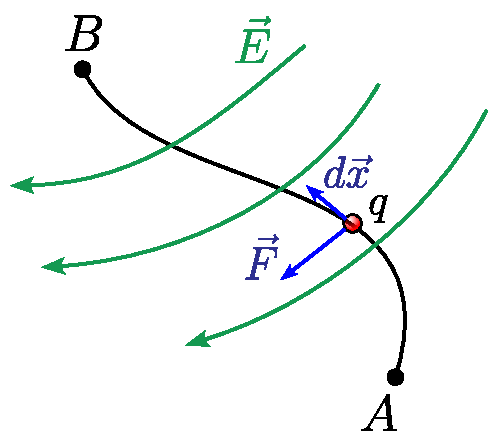
\includegraphics[scale = 0.65]{Figuras/Significado-Potencial.pdf}
    \caption{Interpretación física del potencial.}
    \label{fig:Significado-Potencial}
\end{figure}

La fuerza que actúa sobre la carga en cualquier punto es
$$\vec{F} = q \vec{E}.$$

Entonces, el trabajo efectuado al mover la carga desde $A$ hasta $B$ es 
$$W = - \int_A^B \vec{F} \cdot d\vec{x} = -q \int_A^B \vec{E} \cdot d\vec{x}.$$

El signo menos aparece porque estamos calculando el trabajo hecho sobre la carga  en contra de la acción del campo (trabajo externo). Con la definición \eqref{Relacion-Campo-Potencial}, el trabajo puede ser escrito como
$$W = q \int_A^B \vec{\nabla} \phi \cdot d\vec{x} = q \int_A^B d\phi = q (\phi(B) - \phi(A)).$$

Ésto muestra que $q\phi$ puede ser interpretado como la energía potencial de la carga de prueba en el campo electrostático. 

Finalmente, se tiene una importante relación.
\begin{shaded}
    $$- \int_A^B \vec{E} \cdot d\vec{x} = \phi(B) - \phi(A).$$
\end{shaded}

Se mencionó una energía potencial en el penúltimo párrafo, la cual puede ser asociada a una fuerza conservativa. Por ello, se probará que la fuerza electrostática y por consiguiente el campo electrostático (no dinámico) es conservativo.

Recordemos que
$$\vec{\nabla} \times \vec{E} = \vec{ \nabla} \times (- \vec{\nabla} \phi) = \vec{0}.$$

Usando el teorema de Stokes,
$$\oint_C \vec{E} \cdot d\vec{x} = \iint_S \vec{\nabla} \times \vec{E} \cdot \hat{n} dS = 0,$$

lo cual implica que
$$\oint_C \vec{F} \cdot d\vec{x} = \oint_C q \vec{E} \cdot d\vec{x} = 0.$$

Por lo tanto, $\vec{F}$ es una fuerza conservativa, pues el trabajo realizado en cualquier trayectoria cerrada es cero.

Entonces,
$$W = -\Delta U,$$

donde $U$ es la \textbf{energía potencial eléctrica}.

Por otro lado,
$$-W = -q \int_A^B \vec{E} \cdot d\vec{x} = q \int_A^B \vec{\nabla} \phi \cdot d \vec{x} = \Delta U$$
$$\Rightarrow \qquad \frac{- W}{q} = \int_A^B \vec{\nabla} \phi \cdot d \vec{x} = \frac{\Delta U}{q} = \phi(B) - \phi(A).$$

\newpage
\textbf{Observaciones:}
\begin{enumerate}

\item La diferencia de potencial electrostático lo podemos interpretar como el trabajo realizado para traer una carga desde el punto $A$ hasta el punto $B$ por unidad de carga. 

\item  El potencial electrostático también es llamado \textbf{voltaje} ($V$) y $\Delta V = V_B - V_A$ es la diferencia del voltaje.

\item La unidad de medida es el “Volt”, $1 \,[V] = 1 \, \mbox{Volt} = \frac{1 J}{1C}$.

\item El valor de $\phi$ en una posición no tiene sentido (al igual que en el caso gravitacional, sólo las diferencias de energía potencial tienen significado) a menos que definamos una posición de referencia donde el potencial valga cero. Es usual elegir el punto $A$ en el infinito del tal forma que $\phi(\infty) = 0$. Para así, definir el potencial en un punto $B$ como
$$\phi(B) = - \int_{\infty}^B \vec{E} \cdot d\vec{x}.$$

\textbf{Ojito:} El punto de referencia en el infinito no siempre es una buena elección, por ejemplo, para distribuciones infinitas.

\item No hay que confundir la \textbf{energía potencial electrostática} con \textbf{potencial electrostático}. La energía potencial se mide en \textit{Joule} y es un número único (es trabajo) mientras que el potencial se mide en \textit{Volt} y es diferente en todas partes del espacio.
\end{enumerate}

\section{Potencial eléctrico de cargas puntuales}

El campo eléctrico generado por una carga puntual $q'$ ubicada en el origen está dado por:
$$\Vec{E}(x,y,z) = \frac{1}{4\pi \varepsilon_0} \frac{q'}{(\sqrt{x^2+y^2+z^2})^3} (x \,\hat{\imath} + y \, \hat{\jmath} + z\, \hat{k}).$$

En coordenadas esféricas,
$$\Vec{E}(\Vec{x}) =  \frac{1}{4\pi \varepsilon_0} \frac{q'}{r^2} \, \hat{r}.$$

Como $\vec{E} = - \vec{\nabla} \phi$, se  tiene que
$$\frac{1}{4\pi \varepsilon_0} \frac{q'}{r^2} \, \hat{r} = - \frac{\partial \phi}{\partial r} \,\hat{r} - \frac{1}{r} \frac{\partial \phi}{\partial \theta} \,\hat{\theta} - \frac{1}{r\sin\theta} \frac{\partial \phi}{\partial \varphi} \,\hat{\varphi},$$

donde se escribió el gradiente en coordenadas esféricas. Igualando la componentes, tenemos que
$$\frac{\partial \phi}{\partial r} = -\frac{1}{4\pi \varepsilon_0} \frac{q'}{r^2} \,\wedge\, \frac{\partial \phi}{\partial \theta} = 0 \,\wedge\, \frac{\partial \phi}{\partial \varphi} = 0,$$

es decir, el potencial no depende de $\theta$ y $\varphi$. Entonces, $\phi$ es solo de función de $r$ y por tanto la derivada parcial pasa a escribirse como una derivada ordinaria, ésto es,
$$\frac{d\phi}{dr} =  -\frac{1}{4\pi \varepsilon_0} \frac{q'}{r^2}.$$

Integrando con respecto a $r$,
$$\phi(r) =  \frac{1}{4\pi\varepsilon_0} \frac{q'}{r} + C.$$

Si imponemos que $\phi(\infty) \stackrel{!}{=} 0$, es decir, elegimos como potencial de referencia cero en el infinito, obtenemos que $C = 0$. Luego,
$$\phi(r) =  \frac{1}{4\pi\varepsilon_0} \frac{q'}{r}.$$

Ahora, si consideramos otro sistema coordenado tal que el vector posición de la carga es $\vec{x}\,'$, tenemos que para este sistema, el potencial está dado por
\begin{shaded}
    $$\phi(\Vec{x}) = \frac{1}{4\pi \varepsilon_0} \frac{q'}{|\vec{x} - \Vec{x}\,'|}.$$
\end{shaded}

Podemos interpretar este potencial electrostático como el trabajo que sería realizado sobre una carga $q$ debido a $q'$ para traerla desde el infinito hasta el punto $\Vec{x}$.

Para obtener el potencial eléctrico resultante entre dos o más cargas $q_i$, se aplica el \textit{principio de superposición}. Así, el potencial eléctrico total en $\vec{x}$, es la suma de los potenciales individuales:
\begin{shaded}
    $$\phi(\Vec{x}) = \frac{1}{4\pi \varepsilon_0} \sum_i \frac{q_i}{|\Vec{x} - \Vec{x}_i|},$$
\end{shaded}

donde $\vec{x}_i$ es la posición de la carga $q_i$.

\section{Potencial eléctrico de distribuciones continuas de carga}

Para una distribución continua de carga consideramos un elemento de carga $dq'$ en un volumen $dV'$.

\begin{figure}[H]
    \centering
    \includegraphics[scale = 0.6]{Figuras/Distribucion-Cargas-Potencial.pdf}
    \caption{Distribución de carga.}
    \label{fig:Distribu-Carga-2}
\end{figure}

El potencial en $\Vec{x}$ debido a $dq'$ es
\begin{equation*}
d\phi = \frac{1}{4\pi\varepsilon_0} \frac{dq'}{|\vec{x} - \vec{x}\,'|}.
\end{equation*}

Integrando en todo el volumen,
\begin{shaded}
\begin{equation}
   \phi(\vec{x}) = \frac{1}{4\pi\varepsilon_0} \iiint_{V'} \frac{dq'}{|\vec{x} - \vec{x}\,'|} = \frac{1}{4\pi\varepsilon_0} \iiint_{V'} \frac{\rho(\vec{x}\,')}{|\vec{x} - \vec{x}\,'|} \,dV'. \label{Potencial-Distri}
\end{equation}
\end{shaded}

En la ecuación \eqref{Potencial-Distri} se supuso que se tenía una distribución volumétrica de carga.

\textbf{Observación:} En la expresión del potencial para una carga puntual o una distribución continua estamos suponiendo que $\phi(\infty) = 0$ (válido para toda distribución finita o compacta), pero hay casos en que esa elección no es posible. Siempre hay que tener en mente que lo que se está calculando, es en realidad una diferencia de potencial:
$$\Delta \phi = \frac{1}{4\pi \varepsilon_0} \int \frac{dq'}{|\vec{x} - \vec{x}\,'|}.$$

\subsection{Aplicaciones del potencial}

\begin{ejemplo}
 Un semianillo de radio $R$ tiene una densidad lineal de carga $\lambda(\varphi) =  \frac{A}{R} \sin \varphi$, con $A = cte$, ver figura \ref{fig:Ej-Potencial-1}. Calcular el potencial electrostático sobre el eje $z$ generado por el semianillo.

\begin{figure}[H]
    \centering
    \includegraphics[scale = 0.6]{Figuras/Ej-Potencia-1.pdf}
    \caption{Semianillo de radio $R$ con $\lambda(\varphi) = \frac{A}{R} \sin \varphi$.}
    \label{fig:Ej-Potencial-1}
\end{figure}

\textbf{Solución:} Para calcular el potencial electrostático, se considerará el de referencia cero en el infinito, lo cual es posible ya que la distribución de carga es compacta.

Usando coordenadas cilíndricas, se tiene que
$$dq' = \lambda(\varphi') R \,d\varphi', \quad \vec{x} = z \,\hat{k}, \quad \Vec{x}\,' = R\,\hat{\rho} = R(\cos \varphi'\,\hat{\imath} + \sin \varphi'\,\hat{\jmath}),$$

con $0\leq \varphi' \leq \pi$.

Luego, el diferencial de potencial electrostático en $\vec{x}$ está dado por
\begin{align*}
    d\phi(\Vec{x}) &= \frac{1}{4\pi\varepsilon_0} \frac{dq'}{|\vec{x} - \Vec{x}\,'|} \\
    &= \frac{1}{4\pi\varepsilon_0} \frac{\lambda(\varphi') R}{|z\,\hat{k} - R\,\hat{\rho}|} \,d\varphi' \\
    &= \frac{1}{4\pi\varepsilon_0} \frac{A\sin\varphi'}{\sqrt{z^2 + R^2}} \,d\varphi'.
\end{align*}

Integrando a ambos lados, el potencial electrostático es
\begin{align*}
    \phi(\Vec{x}) &= \int_0^{\pi} \frac{1}{4\pi\varepsilon_0} \frac{A\sin\varphi'}{\sqrt{z^2 + R^2}} \,d\varphi' \\
    &= \frac{1}{4\pi \varepsilon_0} \frac{A}{\sqrt{z^2+R^2}} \int_0^{\pi} \sin \varphi' \,d\varphi' \\
    &= \frac{1}{4\pi \varepsilon_0} \frac{A}{\sqrt{z^2+R^2}} [-\cos\varphi']_0^{\pi} \\
    &=  \frac{1}{2\pi \varepsilon_0} \frac{A}{\sqrt{z^2+R^2}}.
\end{align*}

\end{ejemplo}

\begin{ejemplo} \label{Potencial-Disco}
   Para un disco con densidad de carga constante $\sigma$, radio interior $r$ y radio exterior $R$. Calcule el campo potencial electrostático para el punto $P$, ver figura \ref{fig:Ej-Potencial-2}.

\begin{figure}[H]
    \centering
    \includegraphics[scale = 0.65]{Figuras/Ej-Potencial-2.pdf}
    \caption{Disco de radio interior $r$ y radio exterior $R$ con densidad de carga $\sigma$ constante.}
    \label{fig:Ej-Potencial-2}
\end{figure}

\textbf{Solución:} Para calcular el potencial electrostático, se considerará el de referencia cero en el infinito, lo cual es posible ya que la distribución de carga es compacta.

Usando coordenadas cilíndricas, se tiene que
$$dq' = \sigma \rho' \,d\varphi'\,d\rho',\quad \Vec{x} = z\,\hat{k}, \quad \Vec{x}\,' = \rho' \, \hat{\rho} = \rho' (\cos \varphi'\,\hat{\imath} + \sin \varphi'\,\hat{\jmath}).$$

Luego, el diferencial de potencial electrostático en $\vec{x}$ está dado por
\begin{align*}
    d\phi(\Vec{x}) &= \frac{1}{4\pi\varepsilon_0} \frac{dq'}{|\vec{x} - \Vec{x}\,'|} \\
    &= \frac{1}{4\pi\varepsilon_0} \frac{\sigma \rho' \,d\varphi'\,d\rho'}{|z\,\hat{k} - \rho' \,\hat{\rho}|}\\
    &= \frac{1}{4\pi\varepsilon_0} \frac{\sigma \rho'}{\sqrt{z^2 + \rho'\,^2}} \,d\varphi'\,d\rho'.
\end{align*}

Integrando a ambos lados, el potencial electrostático es
\begingroup
\allowdisplaybreaks
\begin{align*}
    \phi(\Vec{x}) &= \int_r^R \int_0^{2\pi}  \frac{1}{4\pi\varepsilon_0} \frac{\sigma \rho'}{\sqrt{z^2 + \rho'\,^2}} \,d\varphi'\,d\rho' \\
    &= \frac{\sigma}{4\pi \varepsilon_0} \int_r^R \frac{\rho'}{\sqrt{z^2+\rho'\,^2}} \left(\int_0^{2\pi} d\varphi' \right) d\rho' \\
    &= \frac{2\pi \sigma}{4\pi \varepsilon_0} \int_r^R \frac{\rho'}{\sqrt{z^2+\rho'\,^2}}  d\rho' \\
    &= \frac{\sigma}{2\varepsilon_0} \left[ \sqrt{z^2 + \rho'\,^2}\right]_r^R \\
    &= \frac{\sigma}{2\varepsilon_0} \left( \sqrt{z^2 + R^2} - \sqrt{z^2 + r^2}\right).
\end{align*}
\endgroup
  
\end{ejemplo}

\begin{ejemplo}
Calcule el potencial electrostático para cualquier punto en el espacio de la esfera de radio $R$ y con densidad de carga uniforme e igual a $\rho$.

\textbf{Solución:} En la sección \ref{Ley-Gauss} calculamos el campo electrostático de una esfera de radio $R$ y densidad de carga $\rho$, el cual está dado por:
$$\Vec{E}(r) = \left\{ \begin{array}{cl}
   \frac{\rho R^3 }{3\varepsilon_0 r^2} \,\hat{r},  & \text{si} \quad r > R  \\
    \frac{\rho r}{3\varepsilon_0} \,\hat{r}, & \text{si} \quad  0 \leq r < R 
\end{array} \right. .$$

Para calcular el potencial electrostático, recordemos que 
$$\phi(B) - \phi(A) = - \int_A^B \Vec{E} \cdot d\Vec{x}.$$

Como el campo electrostático es conservativo, la integral de línea no depende del camino de integración, por tanto elegiremos la trayectoria que une a un punto $A$ ubicado al infinito con el punto $B$ cualquiera con coordenada esférica $r$ por medio de  un rayo que parte de $A$ hasta $B$. Luego, $d\Vec{x} = dr'\,\hat{r}$ y
$$\phi(r) - \phi(\infty) = - \int_{\infty}^{r} (E(r') \,\hat{r}) \cdot (dr' \,\hat{r}) = -\int_{\infty}^r E(r') \,dr'.$$

Imponiendo $\phi(\infty) \stackrel{!}{=} 0$,
$$\phi(r) = - \int_{\infty}^r E(r') \,dr'.$$

\begin{itemize}
\item[i)] Si $r > R$, 
\begin{align*}
    \phi(r) = - \int_{\infty}^r E(r') \,dr' 
    &= - \int_{\infty}^r \frac{\rho R^3 }{3 \varepsilon_0 r'\,^2} \,  dr' \\
&= - \frac{\rho R^3}{3\varepsilon_0} \int_{\infty}^r \frac{1}{r'\,^2}\, dr' \\
&= - \frac{\rho R^3}{3\varepsilon_0} \left[ - \frac{1}{r'} \right]_{\infty}^r \\
&= \frac{\rho R^3}{3\varepsilon_0 r}.
\end{align*}

\item[ii)] Si $0 \leq r  < R$, 
\begin{align*}
    \phi(r) &= - \int_{\infty}^r E(r') \,dr' \\
    & = - \int_{\infty}^R \frac{\rho R^3}{3 \varepsilon_0 r'\,^2} \, dr' - \int_{R}^r \frac{\rho r'}{3 \varepsilon_0} dr' \\
&= - \frac{\rho R^3 }{3\varepsilon_0} \int_{\infty}^R \frac{1}{r'\,^2} \,dr' - \frac{\rho}{3\varepsilon_0} \int_R^r r' \,dr' \\
&= - \frac{\rho R^3}{3\varepsilon_0} \left[ -\frac{1}{r'} \right]_{\infty}^R - \frac{\rho}{3\varepsilon_0} \left[ \frac{1}{2}r'\,^2 \right]_R^r \\
&= \frac{\rho R^3}{3\varepsilon_0 R} - \frac{\rho}{3\varepsilon_0} \left( \frac{r^2}{2} - \frac{R^2}{2} \right) \\
&= \frac{\rho}{6 \varepsilon_0}(3R^2 - r^2).
\end{align*}

Por lo tanto,
\begin{equation*}
\phi(r) =  \left\{ \begin{array}{cl}
   \frac{\rho R^3 }{3\varepsilon_0 r} ,  & \text{si} \quad r > R  \\
    \frac{\rho}{6\varepsilon_0} (3R^2-r^2), & \text{si} \quad  0 \leq r < R 
\end{array} \right. .
\end{equation*}

\end{itemize}
\end{ejemplo}

\begin{ejemplo}\label{Potencial-Plano-Inf}
     Calcule el potencial electrostático a una distancia $d$, generado por un plano infinito con densidad de carga uniforme y de valor $\sigma$.

\textbf{Solución:} En este caso no podemos asumir que el potencial es cero en el infinito, pues el campo no es débil en el infinito como en el caso de las distribuciones de carga compactas. De hecho, si usamos el potencial de un disco  finito del ejemplo \ref{Potencial-Disco} y tomamos $r = 0$ y el límite cuando $R$ tiende al infinito:
$$\lim_{R \to \infty} \frac{\sigma}{2\varepsilon_0} \left( \sqrt{z^2 + R^2} - z \right) = \infty,$$

es decir, esta ecuación no puede ser usada.

Si consideramos el plano infinito en el plano $xy$, el campo eléctrico está dado por:
\begin{equation*}
\Vec{E}(\Vec{x}) =  \left\{ \begin{array}{cl}
   \frac{\sigma}{2 \varepsilon_0} \,\hat{k} ,  & \text{si} \quad z > 0  \\
    - \frac{\sigma}{2 \varepsilon_0} \,\hat{k}, & \text{si} \quad  z < 0 
\end{array} \right. .
\end{equation*}

De nuevo, para calcular el potencial electrostático, recordemos que
$$\phi(B) - \phi(A) = - \int_A^B \Vec{E} \cdot d\Vec{x}.$$

Elegimos como trayectoria aquella que une al punto $A$ con coordenada $d' \geq 0$ en el eje $z$ mediante un segmento con el punto $B$ con coordenada $z$ igual a $d > 0$. Luego, $d\Vec{x} = dz\,\hat{k}$ y
$$\phi(d) - \phi(d') = - \int_{d'}^{d} (E\,\hat{k}) \cdot (dz\,\hat{k}) = - \int_{d'}^d \frac{\sigma}{2\varepsilon_0} \,dz = - \frac{\sigma}{2\varepsilon}(d-d').$$

Si imponemos, por ejemplo, $\phi(d') \stackrel{!}{=} 0$ en $d' = 0$, tenemos que
$$\phi(d) = - \frac{\sigma}{2\varepsilon_0} d.$$

Si $B$ es un punto con coordenada $z$ igual a $-d$, 
$$\phi(-d)= \frac{\sigma}{2\varepsilon_0} d.$$

Por lo tanto, generalizando para todo punto con coordenada $z$ en el espacio,
$$\phi(z) = - \frac{\sigma}{2\varepsilon_0}|z|.$$

\end{ejemplo}

\subsection{Continuidad de los campos}

En la figura \ref{fig:Campo-Plano-Inf}, están representadas las gráficas del campo eléctrico (sin considerar dirección) y el potencial del plano infinito dados por el ejemplo \ref{Potencial-Plano-Inf}.

    \begin{figure}[H]
        \centering
        \subfigure[]{\includegraphics[width=0.4
        \textwidth]{Figuras/Campo-E-Plano.pdf}} \hspace{1cm}
        \subfigure[]{\includegraphics[width=0.4\textwidth]{Figuras/Potencial-Plano.pdf}} 
        \caption{Gráficas del campo eléctrico (a) y el potencial (b) del plano infinito.}
        \label{fig:Campo-Plano-Inf}
    \end{figure}

Claramente el campo eléctrico presenta una discontinuidad en $z = 0$, es decir, donde se ubica la distribución superficial de carga. Sin embargo, el potencial es continuo en todo el espacio.  

En general, el campo eléctrico y el potencial son continuos para toda distribución volumétrica de carga con densidad $\rho(\Vec{x})$ (finita y continua). Sin embargo, si consideramos distribuciones superficiales de carga ($\rho$ discontinua y divergente), el campo eléctrico tenderá a ser discontinuo en la región donde se ubica la distribución superficial de carga (donde $\rho$ es discontinuo), pero finito en el resto de los puntos del espacio. En cambio el potencial seguirá siendo continuo. En el caso de que la distribución de carga se modele incluyendo cargas puntuales o líneas de carga, el potencial ya no será finito en todo punto.

\section{Energía potencial electrostática}

Consideremos un sistema formado por una carga puntual $q_1$ con vector posición $\Vec{x}_1$, ver figura \ref{fig:Energía-Potencial}-(a). Queremos traer (desde el infinito) una carga puntual $q_2$ hasta la posición $\Vec{x}_2$, para ello debemos efectuar un trabajo en contra del campo eléctrico creado por $q_1$, que está dado por \footnote{Recuerde que $\Delta U = q \Delta \phi$ y hemos supuesto que el cero potencial en el infinito.}
$$U = q_2 \phi_1(\Vec{x}_2) = \frac{1}{4\pi\varepsilon_0}\frac{q_1 q_2}{|\Vec{x}_2 - \Vec{x}_1|},$$

donde $\phi_1$ es el potencial debido a la carga $q_1$.

\textbf{Nota:} Si las cargas tienen igual signo, $U > 0$ y corresponderá a la energía invertida para armar el sistema,  la cual será almacenada y al desarmar el sistema esta será la energía liberada. Por otro lado, si las cargas tienen signos opuestos, $U < 0$ y corresponderá a la energía que se necesitará para desarmar el sistema.

Ahora, si traemos (desde el infinito) otra carga puntual $q_3$ hasta la posición $\Vec{x}_3$, ver figura \ref{fig:Energía-Potencial}, la energía potencial será
$$U_3 = q_3 \phi_1(\vec{x_3}) + q_3 \phi_2(\Vec{x}_3) = \frac{1}{4\pi\varepsilon_0}\frac{q_1 q_3}{|\Vec{x}_3 - \Vec{x}_1|} + \frac{1}{4\pi\varepsilon_0}\frac{q_2 q_3}{|\Vec{x}_3 - \Vec{x}_2|}.$$

Luego, la energía potencial almacenada en el sistema es:
$$U = \frac{1}{4\pi \varepsilon_0} \left(\frac{q_1 q_2}{|\Vec{x}_2 - \Vec{x}_1|} + \frac{q_1q_3}{|\Vec{x}_3-\Vec{x}_1| } + \frac{q_2 q_3}{|\Vec{x}_3 - \Vec{x}_2|} \right).$$

Podemos reescribir la expresión anterior de la forma
\begin{align*}
    U &= \frac{1}{2} \left[q_1 \left( \frac{1}{4\pi \varepsilon_0} \frac{q_2}{|\Vec{x}_2-\Vec{x}_1|} + \frac{1}{4\pi \varepsilon_0} \frac{q_3}{|\Vec{x}_3-\Vec{x}_1|} \right) + q_2 \left( \frac{1}{4\pi \varepsilon_0} \frac{q_1}{|\Vec{x}_1-\Vec{x}_2|} + \frac{1}{4\pi \varepsilon_0} \frac{q_3}{|\Vec{x}_3-\Vec{x}_2|} \right) \right. \\
    &\quad \left. + q_3 \left( \frac{1}{4\pi \varepsilon_0} \frac{q_1}{|\Vec{x}_1-\Vec{x}_3|} + \frac{1}{4\pi \varepsilon_0} \frac{q_2}{|\Vec{x}_2-\Vec{x}_3|} \right) \right].
\end{align*}

\begin{figure}[H]
    \centering
    \includegraphics[scale = 0.65]{Figuras/Energia-Potencial.pdf}
    \caption{Construcción de una configuración de cargas empezando con una carga $q_1$, añadiendo luego una carga $q_2$ (a) y una carga $q_3$ (b).}
    \label{fig:Energía-Potencial}
\end{figure}

Generalizando para $n$ cargas:
\begin{shaded}
  $$U = \frac{1}{2} \sum_{i,j (i\neq j)}^n \frac{1}{4\pi \varepsilon_0} \frac{q_i q_j}{|\Vec{x}_j - \Vec{x}_i|} = \frac{1}{2} \sum_{i,j (i\neq j)}^n q_i \phi_i(\Vec{x}_j),$$ 
\end{shaded}

donde  $\phi_i(\Vec{x}_j)$ es el potencial electrostático en el punto donde se sitúa la carga $q_j$ debido a la carga $q_i$ .

En el caso de una \textit{distribución continua de carga}, la energía potencial almacenada (energía de formación) está dada por:
\begin{shaded}
   $$ U = \frac{1}{2} \iiint_{V} \phi(\Vec{x}) \,dq = \frac{1}{2} \iiint_{V} \rho(\Vec{x}) \phi(\Vec{x}) \,dV, $$
\end{shaded}

donde se ha supuesto una distribución volumétrica de carga.

\begin{ejemplo}
    Encontrar la energía necesaria para formar una esfera de carga total $Q$, de radio $R$ y densidad volumétrica de carga constante $\rho$.

\textbf{Solución:} De la sección anterior, se tiene que el potencial electrostático en un punto dentro de la esfera está dado por:
$$\phi(r)= \frac{\rho}{6 \varepsilon_0}(3R^2 - r^2), \quad 0 \leq r \leq R. $$

Como $\rho = cte$,
$$Q = \rho V = \frac{4}{3} \pi R^3 \rho \Rightarrow  \rho = \frac{3 Q}{4\pi R^3}.$$

Luego,
$$\phi(r)= \frac{Q(3R^2-r^2)}{8 \pi \varepsilon_0R^3}, \quad 0 \leq r \leq R. $$

Usando coordenadas esféricas, se tiene que
$$dV = r^2 \sin \theta \,d\varphi\,d\theta\,dr.$$

Por lo tanto, la energía de formación está dada por
\begin{align*}
    U &= \frac{1}{2} \iiint_V \phi(\Vec{x}) \rho \,dV \\
    &= \frac{1}{2} \rho \int_0^R \int_0^{\pi} \int_0^{2\pi} \frac{Q(3R^2-r^2)}{8 \pi \varepsilon_0 R^3} r^2 \sin \theta \,d\varphi \,d\theta\, dr\\
    &= \frac{Q \rho}{16 \pi \varepsilon_0 R^3} \int_0^R (3R^2 - r^2)r^2 \left(  \int_0^{\pi} \sin \theta \left( \int_0^{2\pi} d\varphi \right) d\theta \right) dr \\
    &=  \frac{2\pi Q \rho}{16 \pi \varepsilon_0 R^3} \int_0^R 3 R^2r^2-r^4 \left( \int_0^{\pi} \sin \theta d\theta  \right) dr \\
    &= \frac{Q \rho}{8 \varepsilon_0 R^3} \int_0^R (3R^2 r^2 -r^4) [- \cos\theta]_0^{\pi} dr \\
&= \frac{Q \rho}{4\varepsilon_0 R^3} \int_0^R 3R^2r^2-r^4 dr \\
&=  \frac{Q \rho}{4\varepsilon_0 R^3} \left[ R^2r^3 - \frac{r^5}{5}  \right]_0^R \\
&= \frac{Q \rho}{4 \varepsilon_0 R^3} \left( R^5 - \frac{R^5}{5}  \right) \\
&= \frac{Q \rho R^2}{5 \varepsilon_0}.
\end{align*}

Reemplazando $\rho = \frac{3 Q}{4\pi R^3}$,
$$U = \frac{3 Q^2}{20 \pi \varepsilon_0 R}.$$
\end{ejemplo}


\section{Superficies equipotenciales}

Tal como las líneas de un campo vectorial proporcionan una manera apropiada de visualizar el campo electroestático para una distribución de cargas, el potencial electroestático en diversos puntos se puede representar gráficamente mediante \textbf{superficies equipotenciales}.

En general:

\begin{itemize}
\item[i)] Las superficies equipotenciales son aquellas en las que todos sus puntos tienen el mismo potencial. En otras palabras,
$$\Delta \phi = 0.$$

Además, puesto que $\Delta U = q \Delta \Phi$, no se efectúa trabajo para mover una partícula cargada $q$ entre dos puntos de la misma superficie equipotencial.

\item[ii)] El campo electroestático $\vec{E}$ es perpendicular a la superficie equipotencial.

En efecto, de la expresión $\phi(B) - \phi(A) = - \int_A^B \vec{E} \cdot d\vec{x}$ podemos decir que cuando una carga efectúa un desplazamiento infinitesimal $d\vec{x}$ a lo largo de una superficie equipotencial, entonces
$$d\phi = \vec{E} \cdot d\vec{x} = 0 \Rightarrow \vec{E} \perp d\vec{x}.$$
\end{itemize} 

\begin{ejemplo}
    Considere dos cargas puntuales $q_1$ y $q_2$, con vectores posición $\Vec{x}_1$ y $\Vec{x}_2$, respectivamente. Encuentre las superficies equipotenciales.

    \textbf{Solución:}  El potencial electroestático en un punto $\Vec{x}$ está dado por
$$\phi(\Vec{x}) = \phi_1(\Vec{x}) + \phi_2(\Vec{x}) = \frac{1}{4\pi\varepsilon_0} \frac{q_1}{|\Vec{x} - \vec{x}_1|} + \frac{1}{4\pi\varepsilon_0} \frac{q_2}{|\Vec{x} - \vec{x}_2|}.$$

Usando coordenadas cartesianas, 
$$\Vec{x} = (x,y,z), \quad \Vec{x}_1 = (x_1,y_1,z_1), \quad \Vec{x}_2 = (x_2,y_2,z_2).$$

\begin{itemize}
\item \textbf{Caso 1}: $q_2 = 0$,
$$\phi = \frac{1}{4\pi\varepsilon_0} \frac{q_1}{\sqrt{(x-x_1)^2 + (y-y_1)^2  + (z-z_1)^2}}.$$

Para encontrar la superficie equipotencial tomemos $\phi = \phi_0 \neq 0$ constante.
$$(x-x_1)^2 + (y-y_1)^2 + (z-z_1)^2 = \left( \frac{1}{4\pi\varepsilon_0} \frac{q_1}{\phi_0} \right)^2.$$

Por lo tanto, las superficies equipotenciales para una carga puntual $q_1$ son esferas centradas en $(x_1,y_1,z_1)$ y radio $q_1/(4\pi\varepsilon_0 \phi_0)$. 

\item \textbf{Caso 2}: Si $q_1 = q_2 \neq 0$, la ecuación que define la superficie está dada por:
\begin{equation*}
 \frac{q_1}{\sqrt{(x-x_1)^2 + (y-y_1)^2  + (z-z_1)^2}} + \frac{q_2}{\sqrt{(x-x_2)^2 + (y-y_2)^2  + (z-z_2)^2}} = cte.
\end{equation*}
\end{itemize}
\end{ejemplo}

En la  figura \ref{fig:SuperficiesEquipotenciales}, las líneas azules corresponden a superficies equipotenciales. En \textcolor{red}{a)} las líneas de campo radiales y las superficies equipotenciales son esferas concéntricas. En \textcolor{red}{b)} y \textcolor{red}{c)} vemos superficies equipotenciales de dos cargas.


\begin{figure}[H]
        \centering
        \subfigure[]{\includegraphics[width=0.37\textwidth]{Figuras/Equipotencial-Carga+.pdf}} \hspace{1cm}
        \subfigure[]{\includegraphics[width=0.37\textwidth]{Figuras/Equipotencial-Carga+-.pdf}} 
        \hspace{1cm}
        \subfigure[]{\includegraphics[width=0.37\textwidth]{Figuras/Equipotencial-Carga++.pdf}} 
        \caption{Campo eléctrico y superficies equipotenciales de una carga puntual positiva (a), de dos cargas con signos opuestos (b) y dos cargas positivas (c). Recuperado de: \href{https://tikz.net/electric_fieldlines2/}{tikz.net}. } \label{fig:SuperficiesEquipotenciales}
    \end{figure}


\section{Ecuación de Poisson y Laplace*}

De la forma diferencial de la ley de Gauss:
$$\Vec{\nabla} \cdot \Vec{E} = \frac{\rho(\Vec{x})}{\varepsilon_0}$$

y recordando que (en electrostática) $\Vec{E} = - \Vec{\nabla} \phi$, podemos combinar estos dos términos
$$\Vec{\nabla} \cdot (- \Vec{\nabla} \phi) = - (\Vec{\nabla} \cdot\Vec{\nabla} ) \phi = \frac{\rho(\Vec{x})}{\varepsilon_0}.$$

Pero, $\Vec{\nabla} \cdot\Vec{\nabla} = \nabla^2$ es el laplaciano. Entonces, el potencial electrostático satisface la \textbf{ecuación de Poisson}
\begin{shaded}
    $$\nabla^2 \phi = - \frac{\rho}{\varepsilon_0}.$$
\end{shaded}

En regiones del espacio donde no se encuentren distribuciones de carga, $\rho \equiv 0$, el potencial satisface la \textbf{ecuación de Laplace}:
\begin{shaded}
    $$\nabla^2 \phi = 0.$$
\end{shaded}

Para resolver cualquiera de las ecuaciones diferenciales, tendremos que hacer consideraciones de simetría, expresar el laplaciano en un sistema coordenado adecuado para facilitar los cálculos y plantear condiciones de borde.

\begin{ejemplo}
    Considere dos cilindros coaxiales muy largos, a diferente potencial, ver figura \ref{fig:CilindrosCoaxiales}. Encontrar el potencial entre los cilindros y el campo eléctrico.

    \begin{figure}[H]
        \centering
        \includegraphics[scale = 0.65]{Figuras/Ej-EcLaplace.pdf}
        \caption{Cilindros coaxiales.}
        \label{fig:CilindrosCoaxiales}
    \end{figure}

    \textbf{Solución:} Dado que los cilindros son extensos bajo un potencial constante, tenemos simetría de traslación con respecto al eje $z$ y simetría de rotación con respecto al eje $z$. Entonces, el potencial no depende de $\varphi$ ni de $z$. La ecuación de Laplace en coordenada cilíndricas es
    $$\nabla^2 \phi = \frac{1}{\rho} \frac{\partial}{\partial \rho}\left(\rho \frac{\partial \phi}{\partial \rho} \right) + \frac{1}{r^2} \frac{\partial^2 \phi}{\partial \varphi^2} + \frac{\partial^2 \phi}{\partial z^2} = 0,$$

    la cual queda reducida a
    $$\frac{1}{\rho} \frac{d}{d\rho}\left( \rho \frac{d \phi}{d\rho} \right) = 0.$$

    Integrando dos veces con respecto a $\rho$, tenemos que
    $$\rho \frac{d\phi}{d\rho} = C_1 \Rightarrow \frac{d \phi}{d\rho} = \frac{A}{\rho} \Rightarrow \phi(\rho) = C_1 \ln(\rho) + C_2,$$

    donde $C_1$ y $C_2$ son constantes de integración. Si imponemos las condiciones de borde: $\phi(a) = \phi_0$ y $\phi(b) = 0$, encontramos que
    $$C_1 = - \phi_0\frac{1}{\ln(b/a)}~\text{y}~ C_2 = \phi_0 \frac{\ln(b)}{\ln(b/a)}.$$

    Por lo tanto,
    $$\phi(\rho) = \phi_0 \frac{\ln(b/\rho)}{\ln(b/a)}.$$

    El campo eléctrico está dado por
    $$\Vec{E} = - \Vec{\nabla} \phi = - \left( \frac{\partial \phi}{\partial \rho} \,\hat{\rho} + \frac{1}{\rho} \frac{\partial \phi}{\partial \varphi} \,\hat{\varphi} + \frac{\partial \phi}{\partial z}\,\hat{k} \right) = \frac{\phi_0}{\rho \ln(b/a)} \,\hat{\rho}.$$
\end{ejemplo}

\section{El momento dipolar eléctrico}

Un \textbf{dipolo eléctrico} es un sistema formado por dos cargas puntuales iguales y de signo contrario y fijas a una distancia $d$. Consideremos entonces dos cargas $+q$ y $-q$ con vectores posición $\Vec{x}_1 = (d/2) \,\hat{k}$ y $\Vec{x}_2 = -(d/2)\,\hat{k}$, ver figura \ref{fig:dipolo}.

El potencial en todo punto del espacio está dado por
$$\phi(\Vec{x}) = \frac{q}{4\pi\varepsilon_0} \left( \frac{1}{|\Vec{x} - \Vec{x}_1|} - \frac{1}{|\Vec{x} - \Vec{x}_2|}\right).$$

Usando coordenadas esféricas, $\Vec{x} = r \,\hat{r} = r(\sin \theta \cos\varphi \,\hat{\imath} + \sin \theta \sin \varphi\,\hat{\jmath} + \cos \theta \,\hat{k})$, tenemos que \footnote{Se obtiene el mismo resultado aplicando el teorema del coseno.}
\begingroup
\allowdisplaybreaks
\begin{align*}
    |\Vec{x} - \Vec{x}_1| &= \sqrt{\left(r\,\hat{r} - \frac{d}{2} \,\hat{k} \right) \cdot\left(r\,\hat{r} - \frac{d}{2} \,\hat{k} \right) } \\
    &= \sqrt{r^2 + \left(\frac{d}{2} \right)^2 - 2 r \left( \frac{d}{2} \right) \hat{r} \cdot \hat{k}} \\
    &= \sqrt{r^2 + \left(\frac{d}{2} \right)^2 - rd \cos\theta} ,\\
     |\Vec{x} - \Vec{x}_2| &= \sqrt{\left(r\,\hat{r} + \frac{d}{2} \,\hat{k} \right) \cdot\left(r\,\hat{r} + \frac{d}{2} \,\hat{k} \right) } \\
    &= \sqrt{r^2 + \left(\frac{d}{2} \right)^2 + 2 r \left( \frac{d}{2} \right) \hat{r} \cdot \hat{k}} \\
    &= \sqrt{r^2 + \left(\frac{d}{2} \right)^2 + rd \cos\theta} .
\end{align*}
\endgroup


Luego, nuestro potencial nos queda
\begin{equation}
  \phi(r,\theta) = \frac{q}{4\pi\varepsilon_0} \left(\frac{1}{\sqrt{r^2 + \left(\frac{d}{2} \right)^2 - rd \cos\theta}} - \frac{1}{\sqrt{r^2 + \left(\frac{d}{2} \right)^2 + rd \cos\theta}} \right). \label{PotencialDipolo}  
\end{equation}

\begin{figure}[H]
    \centering
    \includegraphics[scale = 0.7]{Figuras/DipoloElectrico.pdf}
    \caption{Dipolo eléctrico.}
    \label{fig:dipolo}
\end{figure}

Nos interesa tomar el límite cuando $d \to 0$. Sea la función 
$$f(d) = \frac{1}{\sqrt{r^2 + \left(\frac{d}{2} \right)^2 - rd \cos\theta}}, \quad \text{para} ~ d \ll 1,$$

expandamos en serie de Taylor alrededor de $d = 0$ para $d \ll 1$:
\begin{align*}
    f(d) &= f(0) + f'(0) d + \mathcal{O}(d^2) \\
    &= \frac{1}{r} - \frac{1}{2r^3} (-r \cos\theta) d + \mathcal{O}(d^2) \\
    &= \frac{1}{r} + \frac{d}{2r^2} \cos \theta + \mathcal{O}(d^2) .
\end{align*}

\textbf{Notación:} $\mathcal{O}(d^2)$ significa que los sumando restantes son proporcionales a $d^2$.

Similarmente,
$$\frac{1}{\sqrt{r^2 + \left(\frac{d}{2} \right)^2 + rd \cos\theta}} = \frac{1}{r} - \frac{d}{2r^2} \cos\theta + \mathcal{O}(d^2).$$

Reemplazando en \eqref{PotencialDipolo},
\begin{align*}
   \phi(r, \theta) &= \frac{q}{4\pi\varepsilon}  \left( \frac{1}{r} + \frac{d}{2r^2} \cos \theta - \frac{1}{r} +  \frac{d}{2r^2} \cos \theta \mathcal{O}(d^2) \right) \\
   &= \frac{q}{4\pi \varepsilon_0} \frac{d}{r^2} \cos \theta + \mathcal{O}(qd^2).
\end{align*}

Tomando los límites: $d\to 0$ y $q \to \infty$ tal que $d\cdot q$ sea finito, encontramos que 
$$\phi(r,\theta) \to  \frac{1}{4\pi \varepsilon_0} \frac{qd}{r^2} \cos \theta.$$

La configuración de cargas, bajo estos límites, se conoce como \textbf{dipolo eléctrico ideal} y si definimos el \textbf{momento dipolar eléctrico} como el vector 
$$\Vec{p} := q \Vec{d},$$

donde $\vec{d}$ es un vector de módulo $d$ que va desde la carga negativa a la positiva, tenemos que el potencial del dipolo ideal está dado por
\begin{shaded}
\begin{equation}
   \phi_{dip}(r,\theta) = \frac{p}{4\pi \varepsilon_0} \frac{\cos \theta}{r^2} = \frac{1}{4\pi \varepsilon_0} \frac{\vec{p} \cdot \hat{r}}{r^2}. \label{Potencial-Dipolo-Ideal}
\end{equation}
\end{shaded}

Para obtener el campo eléctrico producido por el dipolo, usaremos el gradiente en coordenadas esféricas.
\begin{align*}
    \Vec{E} &= - \vec{\nabla} \phi \\
    &= - \left( \frac{\partial \phi}{\partial r} \, \hat{r} +  \frac{1}{r} \frac{\partial \phi}{\partial \theta} \, \hat{\theta} + \frac{1}{r\sin\theta} \frac{\partial \phi}{\partial \varphi} \,\hat{\varphi} \right) \\
    &= \frac{1}{4\pi \varepsilon_0} \left(\frac{2p \cos\theta}{r^3} \,\hat{r} + \frac{p \sin\theta}{r^3} \,\theta \right).
\end{align*}

A partir de la figura \ref{fig:MomentoDipolar}, se desprenden las siguientes relaciones:
$$p \cos \theta\,\hat{r} = (\Vec{p} \cdot \hat{r}) \,\hat{r}, \quad p \sin \theta\,\hat{\theta} = - (\Vec{p} - p\cos\theta \,\hat{r}).$$

\begin{figure}[H]
    \centering
    \includegraphics[scale = 0.3]{Figuras/MOmentoDIpolar2.png}
    \caption{Momento dipolar.}
    \label{fig:MomentoDipolar}
\end{figure}

Luego,
\begin{align*}
    \Vec{E} &= \frac{1}{4\pi \varepsilon_0} \frac{1}{r^3} \left(2(\Vec{p} \cdot \hat{r}) \,\hat{r} - (\Vec{p} - p \cos \theta \,\hat{r})  \right) \\
    &=\frac{1}{4\pi \varepsilon_0} \frac{1}{r^3} \left(2(\Vec{p} \cdot \hat{r}) \,\hat{r} - (\Vec{p} - (\Vec{p} \cdot \hat{r}) \,\hat{r})  \right) \\
    &= \frac{1}{4\pi\varepsilon_0} \frac{3(\Vec{p} \cdot \hat{r}) \,\hat{r} - \Vec{p}}{r^3}.
\end{align*}

Por lo tanto, el campo eléctrico de un dipolo ideal está dado por
\begin{shaded}
    $$\Vec{E} = \frac{1}{4\pi \varepsilon_0} \frac{2p \cos\theta\,\hat{r} + p\sin\theta\,\hat{\theta}}{r^3} = \frac{1}{4\pi\varepsilon_0} \frac{3(\Vec{p} \cdot \hat{r}) \,\hat{r} - \Vec{p}}{r^3}.$$
\end{shaded}

\textbf{Observación:} El análisis hecho consideró que la distancia entre las cargas tendía a cero. Queda como ejercicio para el lector verificar que se obtiene el mismo resultado si evaluamos el potencial y el campo eléctrico del dipolo (no ideal) muy lejos, en particular, $d/r \ll 1$. En otras palabras, el dipolo se aproxima a un dipolo ideal muy lejos.

\textbf{Hint:} Expandir en serie de Taylor alrededor de $(d/r) = 0$  la función
$$f\left( \frac{d}{r}\right) = \frac{1}{r\sqrt{1 + \left( \frac{d}{2r}\right)^2 - \frac{d}{r} \cos\theta}}, \quad \text{para} ~ \frac{d}{r} \ll 1.$$

Por último, calculemos el torque sobre un dipolo en un campo externo uniforme.

De la mecánica, sabemos que el torque está dado por $\vec{\tau} = \vec{x} \times \vec{F}$. En el caso del dipolo, se ve que las fuerzas forman una pareja, ver figura \ref{fig:Torque}, de modo que podemos tomar el torque con respecto a $-q$.

\begin{figure}[H]
    \centering
    \includegraphics[scale = 0.7]{Figuras/TorqueDipolo.pdf}
    \caption{Torque de un dipolo.}
    \label{fig:Torque}
\end{figure}

Así, podemos escribir
\begin{shaded}
    $$\vec{\tau} = \vec{d} \times q \vec{E} = q\vec{d} \times \vec{E} = \vec{p} \times \vec{E}.$$
\end{shaded}

\section{Conductores}

Entenderemos por \textbf{conductor}, un material que posee movilidad de un número alto de cargas eléctricas que se encuentran en su interior. Si aplicamos un campo eléctrico sobre este tipo de materiales, estas cargas se pueden mover por el interior del material.

Ahora vamos a examinar un caso especial cuando las cargas en el conductor no se mueven, es decir, están en \textbf{equilibrio electrostático}. Para lograr ésto, se establece que en un conductor (cargado), las cargas (en exceso) se distribuyen de tal manera de reducir la repulsión entre ellas.

\begin{figure}[H]
    \centering
    \includegraphics[scale = 0.6]{Figuras/Conductor.pdf}
    \caption{Conductor sometido a un campo externo (a) para luego entrar en equilibrio electrostático (b).}
    \label{fig:Conductor}
\end{figure}

Un conductor en equilibrio electrostático tiene las siguientes propiedades:

\begin{enumerate}
\item El campo eléctrico dentro  de un conductor en equilibrio electrostático es nulo.

\textbf{Explicación:} Para lograr el equilibrio, las cargas se distribuyen de tal manera que ellas no sufran ninguna fuerza neta. Como consecuencia $\vec{E}_{int} = \vec{0}$, pero al estar las cargas separadas (polarizadas), estas generarían un campo eléctrico que irradia hacia el exterior del conductor.

\item Cualquier carga neta en un conductor aislado debe estar en la superficie, no necesariamente de manera uniforme.

\textbf{Explicación:} Supongamos que tenemos un conductor cargado. Imaginemos una superficie gaussiana muy cercana a la superficie del conductor, ver figura \ref{fig:Gauss-Conductor}.

\begin{figure}[H]
    \centering
    \includegraphics[scale = 0.57]{Figuras/Conductor-Gauss.pdf}
    \caption{}
    \label{fig:Gauss-Conductor}
\end{figure}

La ley de Gauss nos dice que el flujo a través de esa superficie debe ser igual a la carga encerrada:
$$\Phi_{E} = \oiint_S \vec{E} \cdot d\vec{S} = \frac{q_{enc}}{\varepsilon_0}.$$

Pero, puesto que $\vec{E} = \vec{0}$ en el interior, $\Phi_{E} = 0$, y en consecuencia $q_{enc} = 0$. Es decir no hay carga en el interior. Ahora, si colocamos la superficie gaussiana arbitrariamente muy cerca de la superficie conductora, el resultado es el mismo. Por lo tanto, si el conductor está cargado, la carga debe estar necesariamente en la superficie.

\item Si $A$ y $B$ son dos puntos arbitrarios sobre la superficie de un conductor, entonces $\Delta \Phi = \Phi(B) - \Phi(A) = 0$. Ésto implica que el campo eléctrico es perpendicular a la superficie.

\textbf{Explicación:} Si $\Delta \Phi \neq 0$, entonces $d\Phi = \vec{E} \cdot d\vec{x} \neq 0$. Por lo tanto, existiría una componente paralela a la superficie, lo que haría mover a las cargas en contradicción con la condición de equilibrio electrostático.

\item En un conductor de forma irregular, la densidad de carga es mayor donde el radio de curvatura de la superficie es menor.

\textbf{Explicación:} Si un conductor tiene exceso de cargas, éstas se repelerán y tratarán de estar lo más alejadas posible uno de los otras. En superficies planas la repulsión es mayor que si estuvieran en una región con alto grado de curvatura. En regiones con puntas las cargas sentirán menor repulsión entre sí y habrá una mayor densidad de carga en esa región.
\end{enumerate}

\begin{ejemplo}
    Una esfera maciza de radio $a$ y carga $Q$ uniformemente distribuida es blindada por una capa conductora de espesor uniforme $a$. La carga neta de la capa es nula. Calcule el potencial $\phi(r)$ en todo el espacio. Considere $\phi$ nulo infinitamente lejos de la esfera.
    \begin{figure}[H]
        \centering
        \includegraphics[scale = 0.6]{Figuras/Ej-Conductor.pdf}
        \caption{Esfera maciza de radio $a$ y carga $Q$ rodeada por una capa conductora de espesor uniforme $a$.}
        \label{fig:Ej-Conductor}
    \end{figure}
    
    \textbf{Solución:} Primero determinemos el campo eléctrico, para ello usaremos la ley de Gauss aprovechando que el campo es radial por simetría esférica. Como en ejemplos anteriores se desarrollo en detalle este tipo de cálculo, se omitirán pasos.

    Consideremos el cascarón esférico $S$ de radio $r$ centrado en el centro de la esfera maciza. 

    \begin{enumerate}
        \item Para $r > 2a$, 
        $$\oiint_S \Vec{E} \cdot d\Vec{S} = \frac{Q}{\varepsilon_0} \Rightarrow 4\pi r^2 E = \frac{Q}{\varepsilon_0} \Rightarrow \Vec{E}(r) = \frac{Q}{4\pi\varepsilon_0 r^2} \,\hat{r}.$$

        \item Para $a < r < 2a$,
        $$\Vec{E}(r) = \Vec{0}.$$

        \item Para $r< a$,
        $$\oiint_S \Vec{E} \cdot d\Vec{S} = \frac{q_{encerrada}}{\varepsilon_0} \Rightarrow 4\pi r^2 E = \frac{Q r^3}{\varepsilon_0 a^3} \Rightarrow \Vec{E}(r) = \frac{Q r}{4\pi\varepsilon_0 a^3} \,\hat{r}.$$
    \end{enumerate}

    Ahora, calculemos el potencial siguiendo una trayectoria radial desde el infinito hasta un punto con coordenada esférica $r$.

    \begin{itemize}
        \item Para $r > 2a$,
        $$\phi(r) - \phi(\infty) = -\int_{\infty}^r \Vec{E} \cdot d\vec{x} = -\int_{\infty}^r \frac{Q}{4\pi\varepsilon_0 r^2} \,dr = \frac{Q}{4\pi\varepsilon_0 r}.$$

        Si imponemos $\phi(\infty) \stackrel{!}{=} 0$, tenemos que
        $$\phi(r) = \frac{Q}{4\pi\varepsilon_0 r}.$$

        \item Para $a \leq r \leq 2 a$, tenemos que $\Vec{E}(r) = \Vec{0}$. Luego, el potencial es constante y por continuidad, tendrá el mismo valor que en la frontera $r = 2a$, es decir,
        $$\phi(r) = \phi(2a) = \frac{Q}{8\pi\varepsilon_0 a}.$$

        \item Para $r < a$, 
        \begin{align*}
            \phi(r) &= - \int_{\infty}^r E(r) \,dr \\
            &= - \left( \int_{\infty}^{2a} \frac{Q}{4\pi\varepsilon_0 r^2} \,dr + \cancelto{0}{\int_{2a}^a E(r) \,dr} + \int_a^r  \frac{Qr}{4\pi \varepsilon_0 a^3} \,dr \right) \\
            &= \frac{Q}{8\pi \varepsilon_0 a} + \frac{Q(a^2-r^2)}{8\pi \varepsilon_0 a^3}.
        \end{align*}
    \end{itemize}
\end{ejemplo}

\section{Capacitadores}

Un \textbf{capacitor} o \textbf{condensador} está formado por dos conductores aislados eléctricamente uno del otro, ya sea por medio del vacío o un aislante (dieléctrico). Uno con carga $Q$ y el otro $-Q$, ver figura \ref{fig:capacitador}.

\begin{figure}
    \centering
    \includegraphics[scale = 0.55]{Figuras/Capacitador.pdf}
    \caption{Capacitador.}
    \label{fig:capacitador}
\end{figure}

Se puede demostrar experimentalmente que $Q \varpropto V$, y la constante de proporcionalidad $C$ se denomina \textbf{capacitancia} y se escribe como
\begin{shaded}
    $$C = \frac{Q}{|\Delta V|} = \frac{Q}{V}.$$
\end{shaded}

La unidad de medida de la capacitancia es el \textit{Faradio} ($F$) tal que
$$1 \,F  = \frac{1 \,C}{1\,V}.$$

La capacitancia de un capacitador es una propiedad física de dos conductores y depende de: la geometría del capacitor y la permitividad eléctrica $(\varepsilon)$ del medio.

\subsection*{Capacitor de placas paralelas}

Este capacitor consiste en dos placas metálicas paralelas de área $A$, cargadas con una carga $Q$ y separadas por una distancia $d$. Si ignoramos los efectos de borde podemos considerar el campo en el interior uniforme con dirección $\hat{\imath}$, es decir, estamos haciendo la aproximación de dos planos infinitos. 

\begin{figure}[H]
    \centering
    \includegraphics[scale = 0.8]{Figuras/Capacitador-Placas-Paralelas.pdf}
    \caption{Capacitador de placas paralelas.}
    \label{fig:Cap-Placas}
\end{figure}

El campo el eléctrico de un plano infinito ubicado en el plano $x = 0$, está dado por
$$\Vec{E}(x) =  \left\{ \begin{array}{cl}
   \frac{\sigma}{2 \varepsilon_0} \,\hat{\imath} ,  & \text{si} \quad x > 0  \\
    - \frac{\sigma}{2 \varepsilon_0} \,\hat{\imath}, & \text{si} \quad  x < 0 
\end{array} \right. .$$

Por consiguiente, al considerar dos planos infinitos, uno ubicado en el plano $x = 0$ y el otro en el plano $x = d$, tenemos que los campos eléctricos fuera del capacitador se cancelan, sobreviviendo solo el campo entre las placas dado por
$$\Vec{E}(x) = \frac{\sigma}{2\varepsilon_0} \,\hat{\imath} + \frac{\sigma}{2\varepsilon_0} \,\hat{\imath} = \frac{\sigma}{\varepsilon_0} \,\hat{\imath}, \quad 0 < x < d.$$

La diferencial de potencial se obtiene de
$$\Delta V = V(d) - V(0) = - \int_0^d \left(\frac{\sigma}{\varepsilon_0} \,\hat{\imath} \right) \cdot (dx\,\hat{\imath}) = - \int_0^d \frac{\sigma}{\varepsilon_0} dx = - \frac{\sigma}{\varepsilon_0} d.$$

Tomando el valor absoluto de $\Delta V$, la capacitancia es
$$C = \frac{Q}{|\Delta V|} = \frac{\sigma A}{\frac{\sigma}{\varepsilon_0} d} = \frac{\varepsilon_0 A}{d}.$$

\subsection*{Capacitador cilíndrico}

Este capacitador consiste en un cilindro sólido de radio $a$ y carga $+Q$ rodeado coaxialmente por una cáscara cilíndrica de radio $b$ y carga opuesta $-Q$. 

\begin{figure}[H]
    \centering
    \includegraphics[scale = 0.7]{Figuras/Capacitador-Cilindrico.pdf}
    \caption{Capacitador cilíndrico.}
    \label{fig:Cap-Cilindrico}
\end{figure}

Si consideramos el largo $L$ del cilindro lo suficientemente grande, podemos aproximar el campo eléctrico al de un alambre infinito de densidad lineal de carga $\lambda$, a saber,
$$\Vec{E}(\rho) = \frac{\lambda}{2\pi \varepsilon_0 \rho}  \,\hat{\rho}, \quad a < \rho < b.$$

La diferencial de potencial entre los puntos $a$ y $b$ es
$$  \Delta V = - \int_a^b \Vec{E}(\rho) \cdot d\Vec{x}  
= - \int_a^b\frac{\lambda}{2\pi \varepsilon_0 \rho}\, d\rho 
= - \frac{\lambda}{2\pi \varepsilon_0} \int_a^b \frac{1}{\rho} \,d\rho 
= - \frac{\lambda}{2\pi \varepsilon_0} \ln\left( \frac{b}{a} \right).  $$

Entonces, la capacitancia está dada por
$$C =  \frac{Q}{|\Delta V|} = 2\pi \varepsilon_0  \frac{Q}{\lambda\ln\left(  \frac{b}{a}\right)}.$$

Pero, $\lambda = Q/L$. Por lo tanto,
$$C = 2\pi \varepsilon_0  \frac{L}{\ln\left(  \frac{b}{a}\right)}.$$

\subsection*{Capacitador esférico}

Un capacitador esférico consiste de un cascarón conductor de radio $b$ y carga $-Q$ concéntrico con una esfera conductora más pequeña de radio $a$ y carga $+Q$.

\begin{figure}[H]
    \centering
    \includegraphics[scale = 0.7]{Figuras/Capacitador-Esferico.pdf}
    \caption{Capacitador esférico.}
    \label{fig:Cap-Esferico}
\end{figure}

Usando la ley de Gauss se puede encontrar fácilmente el campo eléctrico entre $a$ y $b$:
$$\Vec{E}(r) = \frac{Q}{4\pi \varepsilon_0 r^2} \,\hat{r}, \quad a < r < b.$$

La diferencial de potencial es
$$\Delta V = - \int_a^b \Vec{E}(r) \cdot d\Vec{x} = - \int_a^b \frac{Q}{4\pi \varepsilon_0 r^2} \,dr = - \frac{Q}{4\pi \varepsilon_0 r^2} \left[ - \frac{1}{r}  \right]_a^b = \frac{Q}{4\pi \varepsilon_0} \left( \frac{1}{b} - \frac{1}{a} \right).$$

Note que la diferencia de potencial es negativa. Entonces,
$$|\Delta V| = \frac{Q}{4\pi \varepsilon_0} \left( \frac{1}{a} - \frac{1}{b} \right) = \frac{Q}{4\pi \varepsilon_0} \cdot \frac{b-a}{ab}.$$

Luego, la capitancia es
$$C = \frac{Q}{|\Delta V|} = 4\pi \varepsilon_0 \frac{ab}{b-a}.$$

Note que, con la expresión anterior podemos calcular la capacitancia de un conductor aislado. Si hacemos $b \to  \infty$, la capacitancia queda
\begin{equation*}
C = \lim_{b \to \infty} \left[ 4\pi \varepsilon_0 \frac{ab}{b-a} \right] = 4\pi \varepsilon_0 \lim_{b \to \infty} \left[\frac{a}{1 - \frac{a}{b}} \right] = 4\pi \varepsilon_0 a.
\end{equation*}

\subsection*{Combinaciones de capacitadores}

\begin{enumerate}
\item \textbf{Capacitadores en serie}: En este caso dos o más capacitadores se conectan uno a continuación del otro y se supone que la fuente voltaica se ha aplicado en los extremos de esta combinación. De ello resulta que la carga de ellos es la misma. Nos interesa encontrar la capacitancia total o equivalente, es decir, el valor de la capacitancia de un solo capacitador que podría sustituir a todos los capacitadores del circuito para simplificarlo tal que el circuito resultante sea equivalente al original.

Por simplicidad, consideremos dos capacitadores cualesquiera de capacitancias $C_1$ y $C_2$ con voltajes $V_1$ y $V_2$, respectivamente.

\begin{figure}[H]
    \centering
    \includegraphics[scale = 0.8]{Figuras/Capacitador-Serie.pdf}
    \caption{Capacitadores en serie.}
    \label{fig:Cap-Serie}
\end{figure}

De la definición de capacitancia:
$$C_1 = \frac{Q}{V_1} ~~\text{y}~~ C_2 = \frac{Q}{V_2}.$$

Pero $V_1 + V_2 = V_{ab}$. Luego,
$$V_{ab} = V_1 + V_2 = \frac{Q}{C_1} + \frac{Q}{C_2}.$$

Entonces, la capacitancia equivalente a la combinación es
\begin{align*}
  V_{ab} = V_1 + V_2 
&\Rightarrow  \frac{Q}{C_{eq}} = \frac{Q}{C_1} + \frac{Q}{C_2} \\
&\Rightarrow  \frac{1}{C_{eq}} = \frac{1}{C_1} + \frac{1}{C_2}.  
\end{align*}

Generalizando para $n$ capacitadores en serie:
\begin{shaded}
    $$\frac{1}{C_{eq}} = \sum_{i=1}^n \frac{1}{C_i}$$
\end{shaded}

\item \textbf{Capacitadores en paralelo}: En este caso se unen entre si los extremos de los capacitadores a un lado de ellos y los otros extremos también se unen entre si, ver figura \ref{fig:Cap-Paralelo}. De ello resulta que todos tienen la misma diferencial de potencial.

\begin{figure}[H]
    \centering
    \includegraphics[scale = 0.8]{Figuras/Capacitador-Paralelo.pdf}
    \caption{Capacitadores en paralelo.}
    \label{fig:Cap-Paralelo}
\end{figure}

De la definición de capacitancia:
$$C_1 = \frac{Q}{V_1} ~~\text{y}~~ C_2 = \frac{Q}{V_2}.$$

Como $V_1 = V_2 = V_{ab}$, se tiene que
$$Q_1 = C_1 V_{ab}  ~~\text{y}~~ Q_2 = C_2 V_{ab}.$$

La carga producida se distribuye, es decir, $Q= Q_1 + Q_2$ con $Q = V_{ab} C_{eq}$, entonces
$$V_{ab}C_{eq} = V_{ab} C_1 +  V_{ab} C_2 \Rightarrow C_{eq} = C_1 + C_2.$$

Generalizando para $n$ capacitadores en paralelo:
\begin{shaded}
    $$C_{eq} = \sum_{i=1}^n C_i.$$
\end{shaded}

\end{enumerate}

\subsection*{Energía de un capacitador en el vacío}

Para hacer este cálculo supondremos que  un agente externo lleva elementos de carga $dq$ desde el lado de menor potencial al de potencial mayor (de la placa negativa a la positiva), ésto es, contra del potencial. Consideremos un instante en que la carga del lado positivo es $q$ y que el voltaje entre ambos elementos del capacitador es $V$, dado que el trabajo elemental hecho por la fuerza externa equilibrante es igual al incremento de energía potencial, se tiene que
$$dU = V \,dq = \frac{q}{C} \,dq.$$

Si durante este proceso se transfiere una carga $Q$ de una placa a otra:
$$U = \int_0^Q \frac{q}{C} \,dq = \frac{Q^2}{2C}.$$

Usando $Q = CV$ queda
\begin{shaded}
 \begin{equation*}
U = \frac{1}{2} CV^2
\end{equation*}
\begin{center}
(Energía almacenada en el capacitador)
\end{center}   
\end{shaded}

\subsection*{Densidad de energía eléctrica}

La \textbf{densidad de energía} es la energía  almacenada en un campo eléctrico por unidad de volumen, es decir,
$$u := \frac{dU}{dv}.$$

Si la energía es uniforme, entonces $u = U/v$.

En el caso del campo de un condensador plano:
$$u = \frac{U}{v} = \frac{\frac{1}{2}CV^2}{Ad} = \frac{\frac{1}{2} \left( \frac{\varepsilon_0 A}{d} \right)V^2}{Ad} = \frac{1}{2} \varepsilon_0 \left( \frac{V}{d} \right)^2.$$

Como $V = Ed$,
\begin{shaded}
   $$ u = \frac{1}{2} \varepsilon_0 E^2.$$
\end{shaded}

Este resultado, obtenido para un capacitador plano, se puede generalizar al campo de otros capacitadores, incluso para una esfera.

\begin{ejemplo}
Cosidere una esfera con carga total $Q$ y radio $R$. Si la carga se encuentra distribuida uniformemente, calcule la energía almacenada en la intensidad del campo electrostático generado por la distribución esférica.

\textbf{Solución:} Recordemos que el campo electrostático de una esfera de densidad de carga uniforme de radio $R$, en coordenadas esféricas, está dado por
$$\Vec{E}(r) =  \left\{ \begin{array}{cl}
   \frac{Q}{4\pi \varepsilon_0 r^2} \,\hat{r}  ,  & \text{si} \quad r \geq R  \\
    \frac{Qr}{4\pi \varepsilon_0 R^3}\,\hat{r}, & \text{si} \quad  0 < r < R 
\end{array} \right. .$$

De la definición de densidad de energía:
$$u = \frac{d U}{dv} = \frac{1}{2} \varepsilon_0 E^2 \Rightarrow dU = \frac{1}{2} \varepsilon_0 E^2 dv.$$

Integrando en todo el espacio, usando coordenadas esféricas, se tiene que
\begin{align*}
U &= \int_0^{\infty} \int_0^{\pi} \int_0^{2\pi} \frac{1}{2} \varepsilon_0 E^2 r^2 \sin\theta \,d\varphi \,d\theta \,dr \\
&= \frac{1}{2} \varepsilon_0 \left\{ \int_0^R \int_0^{\pi} \int_0^{2\pi} \frac{Q^2r^2}{16\pi^2 \varepsilon_0^2 R^6} r^2 \sin\theta \,d\varphi\, d\theta \,dr + \int_R^{\infty} \int_0^{\pi} \int_0^{2\pi} \frac{Q^2}{16\pi^2 \varepsilon_0^2 r^4} r^2 \sin\theta \,d\varphi \,d\theta \,dr \right\} \\
&= \frac{Q^2 }{32\pi^2 \varepsilon_0} \left\{ \frac{1}{R^6}\int_0^R r^4 \int_0^{\pi} \sin\theta \int_0^{2\pi} d\varphi \,d\theta \,dr + \int_R^{ \infty} \frac{1}{r^2} \int_0^{\pi} \sin \theta \int_0^{2\pi} d\varphi \,d\theta \,dr \right\} \\
&= \frac{2\pi Q^2}{32 \pi^2 \varepsilon_0} \left\{ \frac{1}{R^6} \int_0^R r^4 \int_0^{\pi} \sin \theta \,d\theta \,dr + \int_R^{\infty} \frac{1}{r^2} \int_0^{\pi} \sin\theta \,d\theta\, dr\right\} \\
&= \frac{2Q^2}{16 \pi \varepsilon_0} \left\{ \frac{1}{R^6} \int_0^R r^4 \,dr + \int_R^{\infty} \frac{1}{r^2} \,dr \right\} \\
&= \frac{Q^2}{8 \pi \varepsilon_0} \left\{ \frac{1}{R^6} \left[ \frac{r^5}{5} \right]_0^R + \left[ - \frac{1}{r} \right]_R^{\infty} \right\} \\
&= \frac{Q^2}{8\pi \varepsilon_0} \left\{ \frac{1}{5R} + \frac{1}{R} \right\} \\
&= \frac{3Q^2}{20\pi \varepsilon_0 R}.
\end{align*}
\end{ejemplo}

\section{Campo eléctrico en la materia}

\subsection{Dieléctricos}

Un material \textbf{dieléctrico} es un aislante que al ser sometido a un campo eléctrico externo ($\vec{E}_0$), éste se poraliza. En otras palabras, se producen desplazamientos de cargas dentro de las moléculas de tal forma que se crean pequeños \underline{dipolos eléctricos}.

\begin{figure}[H]
    \centering
    \includegraphics[scale = 0.5]{Figuras/Dielectrico.pdf}
    \caption{Orientación de los dipolos de un dieléctrico en presencia de un campo eléctrico externo.}
    \label{fig:Dielectrico}
\end{figure}

Las cargas de polarización (dipolos) crean un campo eléctrico en dirección contraria al externo, llamado \textbf{campo de polarización}, $\vec{E}_p$, de manera que el campo total es:
$$\vec{E} = \vec{E}_0 + \vec{E}_p.$$

O en forma escalar 
\begin{equation}
E = E_0 - E_p. \label{CampoTotal}
\end{equation}

El dieléctrico tiene el efecto de disminuir el campo externo y depende del dieléctrico elegido.

Note que con solo la ecuación \eqref{CampoTotal}, no podemos saber el campo total en un dieléctrico, pues hay dos incógnitas ($E$, $E_p$). Aquí, entra la Física proponiendo el siguiente modelo:
$$\vec{E}_p = - \chi \vec{E},$$

donde $\chi$ es definida como una cantidad positiva llamada \textbf{susceptibilidad eléctrica}.

Luego,
$$\vec{E} = \vec{E}_0 - \chi \vec{E} \Rightarrow  (1+\chi)\vec{E} = \vec{E}_0 \Rightarrow  \vec{E} = \frac{\vec{E}_0}{1+\chi}.$$

Se define la \textbf{constante dieléctrica} $\kappa > 1$ como
\begin{shaded}
$$\kappa := 1 + \chi,$$    
\end{shaded}

quedando
\begin{shaded}
  $$\vec{E} = \frac{\vec{E}_0}{\kappa}.$$  
\end{shaded}

A continuación, una tabla con algunas constantes dieléctricas con su respectivo campo de ruptura dieléctrica que simbolizamos con $E_M$. Éste es el máximo campo que soporta el dieléctrico antes de que salte en él una chispa por ionización.

\begin{center}
\begin{tabular}{|c|c|c|}
\hline 
Material & $\kappa$ & $E_M (10^6 \,[V/m])$ \\
\hline 
Vacío & 1.00000 & $\infty$ \\
Aire seco &  1.0006 & 3 \\
Agua & 78 & --- \\
Papel seco & 3.7 & 16 \\
Vidrio & 5.6 & 14 \\
\hline
\end{tabular}
\end{center}

\subsubsection{Capacitador lleno con dieléctrico}

Podemos encontrar fácilmente la relación entre la capacitancia de un capacitador lleno con dieléctrico, de cualquier forma geométrica, con la de uno vacío.

\begin{itemize}
\item[i)] \textbf{Sin dieléctrico}: El capacitador ha sido cargado con voltaje $V_0$ y ha adquirido una carga libre $Q_0$, y después se ha desconectado de la fuente voltaica.

\begin{figure}[H]
    \centering
    \includegraphics[scale = 0.6]{Figuras/Capacitador-Sin-Dielectric.pdf}
    \caption{Capacitador sin dieléctrico.}
    \label{fig:Cap-Sin-Dielectrico}
\end{figure}

La capacidad está dada por
$$C_0 = \frac{Q_0}{V_0} ~~\mbox{en que}~~ V_0 = \int \vec{E}_0 \cdot d\vec{x}.$$

\item[ii)] \textbf{Con dieléctrico}: El mismo capacitador se ha llenado con dieléctrico y al estar desconectado conserva su carga $Q_0$.

\begin{figure}[H]
    \centering
    \includegraphics[scale = 0.6]{Figuras/Capacitador-ConDielectrico.pdf}
    \caption{Capacitador con dieléctrico.}
    \label{fig:Cap-Con-Dielectrico}
\end{figure}

 En este caso,
$$C = \frac{Q_0}{V},$$

donde 
$$V = \int \vec{E} \cdot d\vec{x} = \frac{1}{\kappa}\int \vec{E}_0 \cdot d\vec{x} = \frac{V_0}{\kappa}. $$

Luego,
\begin{shaded}
 $$C = \frac{Q_0}{V_0 / \kappa} = \kappa C_0,$$   
\end{shaded}

es decir, la nueva capacitancia aumentó en un factor $\kappa$. 

Puesto que su voltaje disminuyó, entonces puede adquirir más carga si se aplica de nuevo la fuente. En ese caso,
\begin{equation*}
C = \frac{Q}{V_0} = \kappa C_0 ~~\mbox{y}~~ Q = \kappa C_0 V_0 = \kappa Q_0.
\end{equation*}

\end{itemize}

\begin{ejemplo}
   Calcular la capacitancia de un capacitador plano, de área $A$, separación $d$ y lleno con tres dieléctricos de espesor $d_1$, $d_2$ y $d_3$, y constantes dieléctricas $\kappa_1$, $\kappa_2$ y $\kappa_3$, respectivamente.

\begin{figure}[H]
    \centering
    \includegraphics[scale = 0.7]{Figuras/Ej-Dielectrico.pdf}
    \caption{Capacitador lleno de tres dieléctricos.}
    \label{fig:Ej-Dielectrico}
\end{figure}

\textbf{Solución:} Por definición del potencial electrostático,
\begingroup
\allowdisplaybreaks
\begin{align*}
    V_{ab} = V(a) - V(b) &= \int_0^d \Vec{E} \cdot d\Vec{x} \\
    &= \int_0^d (E \,\hat{\imath}) \cdot (dx\, \hat{\imath}) \\
&= \int_0^d E \,dx \\
&= \int_0^{d_1} \frac{E_0}{\kappa_1} \,dx + \int_{d_1}^{d_1 + d_2} \frac{E_0}{\kappa_2} \,dx + \int_{d_1 + d_2}^{d_1  + d_2 + d_3} \frac{E_0}{\kappa_3} \,dx  \\
&= \frac{E_0}{\kappa_1} d_1 + \frac{E_0}{\kappa_2} d_2 + \frac{E_0}{\kappa_3} d_3.
\end{align*}
\endgroup

Luego, la capacitancia está dada por
$$C = \frac{Q}{V_{ab}} = \frac{Q_0}{\frac{E_0}{\kappa_1} d_1 + \frac{E_0}{\kappa_2} d_2 + \frac{E_0}{\kappa_3} d_3}.$$

Recordando que para un capacitador de placas paralelas: $E_0 = \frac{\sigma_0}{\varepsilon_0}$ y que $Q_0 = \sigma A$. Por lo tanto,
\begin{align*}
    C &= \frac{\sigma_0 A}{\frac{\sigma_0}{\varepsilon_0 \kappa_1} d_1 + \frac{\sigma_0}{\varepsilon_0 \kappa_2} d_2 + \frac{\sigma_0}{\varepsilon_0  \kappa_3} d_3} \\ 
    &= \frac{\varepsilon_0 A}{\frac{d_1}{\kappa_1} + \frac{d_2}{\kappa_2}  + \frac{d_3}{\kappa_3}}.
\end{align*}
  
\end{ejemplo}

\subsubsection{Energía de capacitadores con dieléctrico}

La relación para la energía o de la densidad de energía se mantienen cambiando $\varepsilon_0$ por $\varepsilon = \kappa \varepsilon_0$, ya que las consideraciones físicas en su deducción no cambian.

Así, para un capacitador plano lleno de un dieléctrico vemos que la capacitancia está dada por
$$C = \kappa C_0 = \kappa \varepsilon_0 \frac{A}{d} = \varepsilon \frac{A}{d}.$$

Su energía es
\begin{shaded}
    $$U = \frac{1}{2} C V^2 = \kappa U_0.$$
\end{shaded}

La densidad de energía de un medio dieléctrico es
\begin{shaded}
    $$u = \frac{1}{2} \varepsilon E^2.$$
\end{shaded}

\subsubsection{Densidad de polarización}

La aparición de $\Vec{E}_{p}$ en el capacitor de placas paralelas es equivalente a la aparición de una densidad de carga superficial en ambas caras del dieléctrico, ver figura \ref{fig:densidad-polarizacion}.

\begin{figure}[H]
    \centering
    \includegraphics[scale = 0.7]{Figuras/Densidad-Polarizacion.pdf}
    \caption{Densidad de polarización}
    \label{fig:densidad-polarizacion}
\end{figure}

Usando la ley de Gauss al cilindro de radio $R$ que tiene una tapa en el dieléctrico y la otra tapa dentro del conductor tal que el campo eléctrico sea nulo,
\begin{align*}
    \oiint_S \Vec{E} \cdot d\Vec{S} &= \frac{q_{enc}}{\varepsilon_0} \\
    \int_{S_{tapa}} \Vec{E} \cdot d\Vec{S} &= \frac{1}{\varepsilon_0}\int_0^R \int_0^{2\pi} (\sigma_0 - \sigma_p) \rho\,d\varphi\,d\rho \\
    \int_0^R \int_0^{2 \pi} (E\,\hat{k}) \cdot (\rho \,d\varphi \,d\rho \,\hat{k}) &= \frac{2\pi (\sigma_0 - \sigma_p)}{\varepsilon_0} \int_0^R \rho \,d\rho \\
    \pi R^2 E &= \frac{\pi R^2(\sigma_0 - \sigma_p)}{\varepsilon_0} \\
    E&= \frac{\sigma_0 - \sigma_p}{\varepsilon_0}.
\end{align*}

Pero $E =  \frac{E_0}{\kappa} = \frac{\sigma_0}{\kappa \varepsilon_0}$, entonces igualando 
\begin{shaded}
 \begin{equation}
\sigma_p = \sigma_0 \left(  1- \frac{1}{\kappa} \right) \label{densidadDePolarizacion}
\end{equation}
\end{shaded}

Multiplicando por el área del capacitador, encontramos que la carga de polarización es
\begin{shaded}
    $$q_p = q_0 \left(  1- \frac{1}{\kappa} \right).$$
\end{shaded}

\subsection{Vector de polarización*}

Formalicemos la discusión hecha para materiales dieléctricos. Al estar en presencia de un campo externo, si el dieléctrico esta formado por átomos neutros (o moléculas apolares), el campo inducirá en cada uno un pequeño momento dipolar, apuntando en la misma dirección del campo. Si el dieléctrico está hecho de moléculas polares, cada dipolo permanente experimentará un torque, tendiendo a alinearse en la dirección del campo. 

En los dos casos discutidos se tiene el mismo resultado: varios ``dipolitos'' apuntando en la dirección del campo. El material se dice que se \textit{polariza}. Para medir este efecto definimos al  \textbf{vector de polarización} $\Vec{P}$ como la densidad de momento dipolar,
$$\Vec{P}(\Vec{x}) := ``\lim_{\Delta V \to 0}" \frac{\sum \Vec{p}_i}{\Delta V},$$

donde $\sum\Vec{p}_i$ es el \textit{momento dipolar total de las cargas del material contenidas en el volumen $\Delta V$}. La región con volumen $\Delta V$ se considera centrada en el punto $\Vec{x}$, suficientemente pequeña desde el punto de vista macroscópico, pero grande comparada con la escala determinada por la estructura atómica/molecular del material. 

 \begin{figure}[H]
     \centering
     \includegraphics[scale = 0.6]{Figuras/Polarizacion.pdf}
     \caption{Dipolos en un volumen $\Delta V$.}
     \label{fig:Polarizacion-Volumen}
 \end{figure}

Equivalentemente, el vector de polarización es definido tal que el momento dipolar $d\Vec{p}$ en un elemento de volumen (macroscópico) $dV$ es dado por $d\Vec{p} = \Vec{P}(\Vec{x})\,dV$ \footnote{De forma análoga a la densidad de carga.}. En consecuencia, el momento dipolar total de las cargas contenidas en un volumen $V$ está dado por
$$\Vec{p}_V = \iiint_V \Vec{P}(\Vec{x}) \,dV.$$ 

De la ecuación \eqref{Potencial-Dipolo-Ideal}, tenemos que el potencial generado por un dipolo ideal de momento dipolar $\Vec{p}$ ubicado en el origen es 
$$\phi_{dip}(\Vec{x}) = \frac{1}{4\pi \varepsilon_0} \frac{\Vec{p} \cdot \hat{r}}{r^2} = \frac{1}{4\pi \varepsilon_0} \frac{\Vec{p} \cdot \Vec{x}}{|\Vec{x}|^3},\quad \Vec{x} = r\,\hat{r}.$$

Ahora, si el dipolo se ubica en $\Vec{x}\,'$, efectuamos una traslación de tal forma que el potencial nos queda
$$\phi_{dip}(\Vec{x}) = \frac{1}{4\pi \varepsilon_0} \frac{\Vec{p} \cdot (\Vec{x} - \Vec{x}\,')}{|\Vec{x} - \Vec{x}\,'|^3}.$$

Luego, el potencial generado por una pequeña región de un medio polarizado con elemento de volumen $dV'$ y polarización $\Vec{P}$ es dada por

\begin{figure}[H]
    \centering
    \includegraphics[scale = 0.6]{Figuras/Distribucion-Cargas-Polarizacion.pdf}
    \caption{Distribución de carga.}
    \label{fig:Distribu-Carga-3}
\end{figure}

$$d\phi(\Vec{x}) = \frac{1}{4\pi\varepsilon_0} \frac{\Vec{P}(\Vec{x}\,') \cdot (\Vec{x} - \Vec{x}\,') \,dV'}{|\Vec{x} - \Vec{x}\,'|^3}.$$

Por lo tanto, el potencial (macroscópico), bajo el modelo de considerar el dieléctrico como una ``nube" de dipolos ideales, está dado por 
\begin{shaded}
    $$\phi(\Vec{x}) = \frac{1}{4\pi \varepsilon_0} \iiint_V \frac{\Vec{P}(\Vec{x}\,') \cdot (\Vec{x} - \Vec{x}\,') }{|\Vec{x} - \Vec{x}\,'|^3} \,dV'$$
\end{shaded}

Usando la identidad \eqref{Identidad-Grad}, podemos escribir
\begin{align*}
    \frac{\Vec{P}(\Vec{x}\,') \cdot (\Vec{x} - \Vec{x}\,')}{|\Vec{x} - \vec{x}\,'|^3} &= \Vec{P}(\Vec{x}\,') \cdot \Vec{\nabla}\,' \left( \frac{1}{|\Vec{x} - \Vec{x}\,'|^3} \right) \\
    &= \Vec{\nabla}\,' \cdot \left( \frac{\Vec{P}(\vec{x}\,')}{|\Vec{x} - \Vec{x}\,'|} \right) - \frac{\Vec{\nabla}\,' \cdot \Vec{P}(\Vec{x}\,')}{|\Vec{x} - \Vec{x}\,'|},
\end{align*}

donde $\Vec{\nabla}\,'$ es el operador nabla con las derivadas parciales con respecto a las coordenadas primas $(x',y',z')$ en el dieléctrico.  

Sea $S'$ la superficie que encierra al volumen $V'$ con elemento de superficie $d\Vec{S}' = \hat{n} dS'$, por el teorema de Gauss,
\begin{align*}
    \phi(\Vec{x}) &= \frac{1}{4\pi\varepsilon_0} \left[ \iiint_{V'} \Vec{\nabla}\,' \cdot \left( \frac{\Vec{P}(\vec{x}\,')}{|\Vec{x} - \Vec{x}\,'|} \right) \,dV' -  \iiint_{V'} \frac{\Vec{\nabla}\,' \cdot \Vec{P}(\Vec{x}\,')}{|\Vec{x} - \Vec{x}\,'|} \,dV'\right] \\
    &= \frac{1}{4\pi \varepsilon_0} \iint_{S'}  \frac{\Vec{P}(\vec{x}\,') \cdot \hat{n}}{|\Vec{x} - \Vec{x}\,'|} \,dS' - \frac{1}{4\pi \varepsilon_0} \iiint_{V'} \frac{\Vec{\nabla}\,' \cdot \Vec{P}(\Vec{x}\,')}{|\Vec{x} - \Vec{x}\,'|} \,dV'.
\end{align*}

El primer término se ve como el potencial de una superficie cargada con densidad de carga
\begin{shaded}
    $$\sigma_p := \vec{P} \cdot \hat{n},$$
\end{shaded}

mientras que el segundo término se ve como el potencial de un volumen con densidad de carga
\begin{shaded}
    $$\rho_p := - \Vec{\nabla} \cdot \Vec{P}.$$
\end{shaded}

Así, el potencial total es 
\begin{shaded}
    $$\phi(\Vec{x}) = \frac{1}{4\pi \varepsilon_0} \iint_{S'}  \frac{\sigma_p(\vec{x}\,')}{|\Vec{x} - \Vec{x}\,'|} \,dS' + \frac{1}{4\pi \varepsilon_0} \iiint_{V'} \frac{\rho_p(\Vec{x}\,')}{|\Vec{x} - \Vec{x}\,'|} \,dV'.$$
\end{shaded}


\textbf{Observación:} Note que la carga total de polarización, tal como se espera, es nula:
$$Q_p = \iiint_V \rho_p \,dV + \oiint_{S} \sigma_p \,dS = \iiint_V \Vec{\nabla} \cdot \Vec{P} \,dV - \iiint_{V} \Vec{\nabla} \cdot \Vec{P}  \,dV = 0,$$

donde se usó el teorema de Gauss.

\begin{ejemplo}
    Considere una esfera de radio $R$ polarizada radialmente con
    $$\Vec{P} = P_0 \,\hat{r},$$

    donde $P_0$ es una constante.
    \begin{itemize}
        \item[(a)] Calcule las densidades de polarización $\sigma_p$ y $\rho_p$.

        \item[(b)] Encuentre el campo eléctrico en el interior y exterior de la esfera.
    \end{itemize}
    
    \textbf{Solución:} En el interior de la esfera, 
    $$\rho_p = - \Vec{\nabla} \cdot \Vec{P} = - \frac{1}{r^2} \frac{d}{dr}(r^2 P_0) = - \frac{2P_0}{r}, \quad r < R,$$

    y nulo en el exterior. La densidad superficial de carga es
    $$\sigma_p = \Vec{P} \cdot \hat{n} = ( P_0 \,\hat{r}) \cdot \hat{r} = P_0.$$

     \begin{figure}[H]
        \centering
        \includegraphics[scale = 0.65]{Figuras/Ej-Polarizacion.pdf}
        \caption{Esfera polarizada radialmente.}
        \label{fig:Esfera-Polarizada-Radial}
    \end{figure}

    Ahora calculemos el campo eléctrico, para ello determinaremos el campo eléctrico de una distribución de carga con 
    $$\rho_p = \left\{\begin{array}{cl}
        -\frac{2P_0}{r}, & \mbox{si} ~ r < R  \\
        0, & \mbox{si} ~ r > R  
    \end{array} \right., \quad \sigma_p = P_0 \quad (r = R),$$

    y nos aprovecharemos de que la distribución posee simetría esférica.

    Luego podemos suponer que el potencial eléctrico sólo depende de la coordenada $r$: $\phi = \phi(r)$ y, en consecuencia, el campo eléctrico es radial, pues
    $$\Vec{E} = - \Vec{\nabla} \phi = - \frac{d \phi}{dr} \,\hat{r} = E(r) \,\hat{r}.$$

    Usando la ley de Gauss a una superficie $S$ esférica de radio $r$ concéntrica con la esfera dieléctrica, el flujo del campo eléctrico es
    $$\oiint_S \Vec{E} \cdot d\Vec{S} = \iint E(r) \,dS = 4\pi r^2 E.$$

    \begin{itemize}
        \item Si $r < R$, por la ley de Gauss,
        $$4\pi r^2 E = \frac{q_{enc}}{\varepsilon_0} = \frac{1}{ \varepsilon_0} \iiint_{r < R} \rho_p \,dV.$$

        La carga encerrada es
        \begin{align*}
            q_{enc} = \iiint_{r < R} \rho_p \,dV &= \int_0^r \int_0^{\pi} \int_0^{2\pi} \left( - \frac{2P_0}{r'}\right) r'\,^2 \sin \theta \,d\varphi \,d\theta \,dr' \\
            &= - 8\pi P_0 \int_0^r r' \,dr' \\
            &= - 4\pi P_0 r^2
        \end{align*}

        y el campo eléctrico está dado por
        $$4\pi r^2 E = - \frac{4\pi P_0 r^2}{\varepsilon_0} \Rightarrow \Vec{E} = - \frac{P_0}{\varepsilon_0} \, \hat{r} = - \frac{\Vec{P}}{\varepsilon_0}.$$

        \item Si $r > R$, debemos tener en consideración la carga en el volumen como en la superficie, la cual es nula por lo demostrado. Entonces,
        $$\Vec{E} = \Vec{0}, \quad r  > R.$$
    \end{itemize}

    Combinando ambos resultados,
    $$\Vec{E} = \left\{\begin{array}{cl}
        -\frac{\Vec{P}}{\varepsilon_0}, & \mbox{si} ~ r < R  \\
        0, & \mbox{si} ~ r > R  
    \end{array} \right..$$
\end{ejemplo}

\subsection{Vector de desplazamiento*}

Vimos que cuando un dieléctrico está polarizado, aparece una densidad volumétrica de carga $\rho_p$. Esta densidad genera a su vez un campo eléctrico, el cual se superpone a cualquier otro campo eléctrico presente. Este campo es generado por, lo que llamaremos, \textbf{cargas libres} (o \textbf{externas}), con densidad de carga $\rho_{libre}$. Entonces, dentro del dieléctrico, la densidad de carga puede ser escrita como:
$$\rho =  \rho_{libre} + \rho_p,$$

y usando la forma diferencial de la ley de Gauss, tenemos que el campo eléctrico total (no solo el generado por la polarización) verifica que 
$$\Vec{\nabla} \cdot \Vec{E} = \frac{1}{\varepsilon_0} (  \rho_{libre} + \rho_p).$$


Pero, $\rho_{p} = - \Vec{\nabla} \cdot \Vec{P}$. Luego,
$$\Vec{\nabla} \cdot \Vec{E} = \frac{1}{\varepsilon_0} (\rho - \Vec{\nabla} \cdot \vec{P}).$$

Reordenando,
$$\Vec{\nabla} \cdot ( \varepsilon_0 \Vec{E} + \Vec{P}) = \rho_{libre}.$$

La expresión entre paréntesis se conoce como el \textbf{vector de desplazamiento eléctrico},
\begin{shaded}
    $$\Vec{D} := \varepsilon_0 \Vec{E} + \Vec{P}.$$
\end{shaded}

Por lo tanto, en términos de $\Vec{D}$, la forma diferencial de la ley de Gauss se puede escribir, de forma más general, como
\begin{shaded}
    $$\Vec{\nabla} \cdot \Vec{D} = \rho_{libre}.$$
\end{shaded}

Usando el teorema de Gauss, es directo probar la forma integral,
\begin{shaded}
    $$\oiint_S \Vec{D} \cdot d\Vec{S} = q_{libre},$$
\end{shaded}

donde $q_{libre}$ denota la carga total libre encerrada en el volumen.

\subsection{Susceptibilidad eléctrica y constante dieléctrica*}

El grado de polarización de un dieléctrico va a depender de la naturaleza molecular del dieléctrico y también del campo eléctrico aplicado. A nivel macroscópico, experimentalmente se ha encontrado que $\Vec{P}$ depende de $\Vec{E}$, $\Vec{P} = \Vec{P}(\Vec{E})$, es decir, si el campo eléctrico varía en todo punto del material, entonces así lo hará el vector de polarización.

La forma más sencilla es cuando el material es \textbf{lineal} e \textbf{isotrópico}. El material se dice lineal si  $\Vec{P}$ depende linealmente de $\Vec{E}$ e isotrópico si éste no posee ninguna dirección preferente. Por lo tanto, la polarización debe necesariamente ser paralela al campo eléctrico, independientemente de la dirección de este último. Luego, podemos escribir 
\begin{shaded}
    $$\Vec{P} = \varepsilon_0 \chi \Vec{E},$$
\end{shaded}

donde, de nuevo, $\chi$ es la \textbf{susceptibilidad eléctrica} del material .\footnote{Para materiales no isotrópicos (anisotrópicos), pero lineales, la relación es idéntica salvo que $\chi$ pasa a ser un tensor.}

\textbf{Observación:} Es importante destacar que $\chi$ puede depender de la posición, $\chi = \chi(\Vec{x})$, pero si el medio es además homogéneo, $\chi$ no depende de la posición, es decir, es constante.

Muchos materiales presentan propiedades de polarización independientes de la dirección del campo eléctrico, es decir, son isótropos. Por ejemplo, los gases, líquidos (excepto los, así llamados, cristales líquidos), sólidos amorfos (plásticos, vidrio).

Ahora, si combinamos esta ecuación con $\Vec{D} = \varepsilon_0 \Vec{E} + \Vec{P}$,
$$\Vec{D} = \varepsilon_0 \Vec{E} + \varepsilon_0 \chi \Vec{E} = \varepsilon_0 (1 +\chi) \Vec{E}$$

y definimos la \textbf{permitividad eléctrica} del material como
\begin{shaded}
$$\varepsilon := \varepsilon_0 (1 +\chi) $$    
\end{shaded}

de tal forma que el desplazamiento toma la forma
$$\Vec{D} = \varepsilon \Vec{E}.$$

Anteriormente ya habíamos introducido la constante dieléctrica $\kappa$, la cual ahora podemos relacionar con $\varepsilon$
$$\varepsilon = \kappa \varepsilon_0.$$

Como $\kappa$ es una cantidad adimensional, es más conveniente trabajar con ella
$$\kappa = \frac{\varepsilon}{\varepsilon_0} = 1 + \chi.$$

Por lo tanto, para un medio lineal
\begin{shaded}
    $$\Vec{P} = (\kappa - 1)\varepsilon_0 \Vec{E} = (\varepsilon - \varepsilon_0) \Vec{E} ~~\text{y}~~ \Vec{D} = \kappa\varepsilon_0 \Vec{E}.$$
\end{shaded}

\textbf{Observación:} El vacío puede ser considerado como ``medio isótropo"\, con $\chi = 0$ y $\kappa = 1$, es decir, no polarizable.

\begin{ejemplo}
    Consideremos una carga $q$ localizada en el origen y sumergida en un dieléctrico de extensión infinita y constante $\kappa$. Encontrar el campo eléctrico en el dieléctrico.

    \begin{figure}[H]
        \centering
        \includegraphics[scale = 0.55]{Figuras/Ej-Isotropico.png}
        \caption{Carga en un medio dieléctrico. 
 Recuperado de \cite{Alvarez} en la pág. 128. }
        \label{fig:Carga-Dielectrico}
    \end{figure}

    \textbf{Solución:} Si suponemos que el material es lineal e isotrópico, los vectores $\Vec{E}$, $\Vec{D}$ y $\Vec{P}$ son paralelos. Por simetría esférica, el campo eléctrico es radial, así que
    $$\Vec{D} = D(r)  \,\hat{r}, \quad \Vec{E} = E(r) \,\hat{r}, \quad \Vec{P} = P(r) \,\hat{r}.$$

    Usando la ley de Gauss para una superficie gaussiana esférica de radio $r$ con origen en la carga $q$,
    \begin{align*}
       \oiint_S \Vec{D} \cdot d\Vec{S} &= q_{libre} \\
       \int_0^{\pi} \int_0^{2\pi} (D(r) \,\hat{r}) \cdot (r^2 \sin \theta \,d\varphi \,d\theta) &= q \\
       4\pi r^2 D(r) &= q \\
       D(r) &= \frac{q}{4\pi r^2}.
    \end{align*}

    Entonces,
    $$\Vec{D} = \frac{q}{4\pi r^2} \,\hat{r}.$$

    El campo eléctrico se obtiene de $\Vec{D} = \varepsilon \Vec{E} = \kappa \varepsilon_0 \Vec{E}$,
    $$\Vec{E} = \frac{q}{4\pi \kappa \varepsilon_0 r^2} \,\hat{r}.$$

    Por último, el vector de polarización está dado por
    $$\Vec{P} = (\kappa -1) \varepsilon_0 \Vec{E} = \frac{(\kappa-1)q}{4\pi \kappa r^2} \,\hat{r}.$$
\end{ejemplo}

\subsection{Condiciones de borde*} \label{sec:Cond-Borde-Dielectricos}

Consideremos dos dieléctricos separados por una superficie de frontera, ver figura \ref{fig:Borde-Normal}. Queremos saber como cambian los vectores $\Vec{E}$ y $\Vec{D}$ cuando estos cruzan la frontera. 

\begin{figure}[H]
    \centering
    \includegraphics[scale = 0.6]{Figuras/Condicion-Borde-Normal.pdf}
    \caption{Condición de borde para la componente normal.}
    \label{fig:Borde-Normal}
\end{figure}

Si ampliamos la superficie, ésta se aproximará a un plano de tal forma que la densidad de carga (libre) y $\Vec{D}$ sean constantes. Aplicamos la ley de Gauss usando como superficie $S$ el cilindro de la figura \ref{fig:Borde-Normal}. 
$$\oiint_S \Vec{D} \cdot d\Vec{S} = q_{libre}.$$

Como $\sigma_{libre}$ se puede considerar constante, la carga libre encerrada $q_{libre} = \sigma_{libre} \Delta S$, luego separando las superficies que constituyen el cilindro,
\begin{equation}
\iint_{S_1} \Vec{D}_1 \cdot d\Vec{S} + \iint_{S_2} \Vec{D}_2 \cdot d\Vec{S} + \iint_{S_3} \Vec{D} \cdot d\Vec{S} = \sigma_{libre} \Delta S,    \label{Borden-Normal}
\end{equation}

donde $S_1$ es la tapa inferior, $S_2$ la tapa superior y $S_3$ el manto del cilindro. 

Ahora, si $\Delta h \to 0$, la integral $\int_{S_3} \Vec{D} \cdot d\Vec{S}$, que es proporcional a $\Delta h$, se anula en este límite. Además, si consideramos $\hat{n}$ el vector unitario normal a la superficie que apunta desde la región 1 hasta la región 2, la ecuación \eqref{Borden-Normal} nos queda:
\begin{align*}
    -(\Vec{D}_1 \cdot \hat{n}) \iint_{S_1} dS + (\Vec{D}_2 \cdot \hat{n}) \iint_{S_2} dS &= \sigma_{libre} \Delta S \\
    -(\Vec{D}_1 \cdot \hat{n}) \Delta S + (\Vec{D}_2 \cdot \hat{n}) \Delta S &= \sigma_{libre} \Delta S \\
    -(\Vec{D}_1 \cdot \hat{n}) + (\Vec{D}_2 \cdot \hat{n}) &= \sigma_{libre}.
\end{align*}

Por lo tanto,
\begin{shaded}
\begin{equation}
  \Vec{D}_2 \cdot \hat{n} - \Vec{D}_1 \cdot \hat{n} = \sigma_{libre}.  \label{Componente-Normal}
\end{equation}
\end{shaded}

La expresión \eqref{Componente-Normal} nos quiere decir que la componente normal de $\Vec{D}$ es discontinua en una interfase entre dos dieléctricos siempre y cuando exista una carga superficial.

\textbf{Observación:} Si los medios son lineales e isotrópicos $\Vec{D} = \varepsilon \Vec{E}$ y las regiones 1 y 2 tienen permitividades $\varepsilon_1$ y $\varepsilon_2$, respectivamente, se cumple
$$\varepsilon_2 \Vec{E}_2 \cdot \hat{n} - \varepsilon_1 \Vec{E}_1 \cdot \hat{n} = \sigma_{libre}.$$

Para el vacío, $\varepsilon_1 = \varepsilon_2 = \varepsilon_0$
$$\Vec{E}_2 \cdot \hat{n} - \Vec{E}_1 \cdot \hat{n} = \frac{\sigma}{\varepsilon_0},$$

donde hemos denotado $\sigma_{libre}$ simplemente como $\sigma$.

Por otro lado, estudiemos qué sucede con la componente tangencial del campo eléctrico. 

\begin{figure}[H]
    \centering
    \includegraphics[scale = 0.6]{Figuras/Condicion-Borde-Tangencial.pdf}
    \caption{Condición de borde para la componente tangencial.}
    \label{fig:Borde-Tangencial}
\end{figure}

Como el campo eléctrico es conservativo (en electrostática), la integral de línea siguiendo cualquier curva cerrada es cero. En nuestro caso elegimos el camino rectangular $abcd$ de la figura \ref{fig:Borde-Tangencial}.
$$\oint_{abcd} \Vec{E} \cdot \,d\Vec{x} = 0.$$

 Descomponemos la trayectoria en los segmentos $ab$, $bc$, $cd$ y $da$:
\begin{equation}
\int_{ab} \Vec{E} \cdot d\Vec{x} + \int_{bc} \Vec{E} \cdot d\Vec{x} + \int_{cd} \Vec{E} \cdot d\Vec{x} + \int_{da} \Vec{E} \cdot d\Vec{x} = 0.   \label{Borden-Tangencial}
\end{equation}

Ahora, si $\Delta h \to 0$, las integrales $\int_{bc} \Vec{E} \cdot d\Vec{x}$ y  $\int_{da} \Vec{E} \cdot d\Vec{x}$, que son proporcionales a $\Delta h$, se anula en este límite. Además, si consideramos $\hat{t}$ un vector tangencial a la superficie que apunta en el mismo sentido que el segmento $ab$, la ecuación \eqref{Borden-Tangencial} nos queda:
\begin{align*}
    (\Vec{E}_2 \cdot \hat{t}) \int_{ab} dx - (\Vec{E}_1 \cdot \hat{t}) \int_{cd} dx &= 0 \\
    (\Vec{E}_2 \cdot \hat{t}) \Delta l - (\Vec{E}_1 \cdot \hat{t}) \Delta l &= 0 .
\end{align*}

Por lo tanto, 
\begin{shaded}
\begin{equation}
    \Vec{E}_2 \cdot \hat{t} = \Vec{E}_1 \cdot \hat{t}.    \label{Componente-Tangencial}
\end{equation}
\end{shaded}

Dado que la dirección del vector $\hat{t}$ es arbitraria (pero siempre tangencial a la superficie), la condición \eqref{Componente-Tangencial} implica que las componentes tangenciales (2 componentes linealmente independientes) del campo eléctrico permanecen inalteradas al cruzar la superficie, es decir, la componente tangencial del campo eléctrico es continua.

\begin{ejemplo} \label{Ej-Cond-Borde}
Una esfera conductora de radio $R$ flota hasta la mitad en un medio dieléctrico de permitividad eléctrica $\varepsilon_1$. La región sobre la esfera es un gas de permitividad eléctrica $\varepsilon_2$. La esfera está carga con una carga igual a $Q$.

\begin{figure}[H]
    \centering
    \includegraphics[scale = 0.45]{Figuras/Ej-Condicion-Borde.png}
    \caption{Esfera conductora sumergida en dos dieléctricos.}
    \label{fig:Ej-Condicion-Borde}
\end{figure}

\begin{itemize}
    \item[(a)] Calcule el campo eléctrico en todo el espacio. 

    \item[(b)] Calcule la densidad de carga libre superficial en la esfera conductora, y la densidad superficial de carga de polarización de ambos medios dieléctricos en la interfaz con la esfera.
\end{itemize}

\textbf{Solución:} Primero elegimos un sistema coordenado como el de la figura \ref{fig:Ej-Condicion-Borde-1}.

\begin{figure}[H]
    \centering
    \includegraphics[scale = 0.6]{Figuras/Ej-Condicion-Borde.pdf}
    \caption{Sistema coordenado.}
    \label{fig:Ej-Condicion-Borde-1}
\end{figure}

\begin{itemize}
    \item[(a)] Para $r < R$, se tiene que $\Vec{E} = \Vec{0}$ ya que es un conductor. Para $r > R$, usaremos la ley de Gauss, teniendo en cuenta que $\Vec{D} = D(r) \,\hat{r}$ y la superficie Gaussiana $S$ esférica de radio $r$ centrada en la esfera conductora. Así,
    $$\oiint_S \Vec{D} \cdot d\Vec{S} =  q_{libre} \Rightarrow \int_0^{\pi} \int_0^{2\pi} D(r) r^2 \sin \theta \,d\varphi \,d\theta = Q.$$

    Si $\Vec{D}_1$ y $\Vec{D}_2$ son los vectores de desplazamiento de los dieléctricos con permitividad eléctrica  $\varepsilon_1$ y $\varepsilon_2$, respectivamente, tenemos que
    \begin{align*}
     \int_0^{\pi/2} \int_0^{2\pi} D_2(r) r^2 \sin \theta \,d\varphi \,d\theta + \int_{\pi/2}^{\pi} \int_0^{2\pi} D_2(r) r^2 \sin \theta \,d\varphi \,d\theta &= Q\\
    \Rightarrow \quad D_2(r) \cdot 2\pi r^2 + D_1(r) \cdot 2\pi r^2 &= Q.   
    \end{align*}

    Ahora, debido a la simetría, el campo eléctrico es completamente tangente a la interfase de los medios, ver figura \ref{fig:Ej-Condicion-Borde-2}. Entonces, $\Vec{E}_1 = \Vec{E}_2 = \Vec{E}$. Además, $D_1(r) = \varepsilon_1 E(r)$ y $D_2(r) = \varepsilon_2 E(r)$. Por lo tanto, el campo eléctrico, para $r > R$, está dado por
    $$\Vec{E}(r) = \frac{Q}{2\pi r^2(\varepsilon_1 + \varepsilon_2)} \,\hat{r}.$$

    \begin{figure}[H]
    \centering
    \includegraphics[scale = 0.6]{Figuras/Ej-Condicion-Borde-2.pdf}
    \caption{Vectores de desplazamiento (a) y el campo eléctrico (b) de una esfera sumergida en dos dieléctricos.}
    \label{fig:Ej-Condicion-Borde-2}
\end{figure}
    
    \item[(b)] La densidad de carga libre dependerá del hemisferio de la esfera. Entonces, para el hemisferio inferior:
    $$\sigma_{l1} = \left.\vec{D}_1(r) \cdot \hat{n} \right|_{r = R} = \frac{\varepsilon_1Q}{2\pi R^2(\varepsilon_1 + \varepsilon_2)} \hat{r} \cdot \hat{r} = \frac{\varepsilon_1Q}{2\pi R^2(\varepsilon_1 + \varepsilon_2)}$$

    y para el hemisferio superior:
     $$\sigma_{l2} = \left.\vec{D}_2(r) \cdot \hat{n} \right|_{r = R} = \frac{\varepsilon_2Q}{2\pi R^2(\varepsilon_1 + \varepsilon_2)} \hat{r} \cdot \hat{r} = \frac{\varepsilon_2Q}{2\pi R^2(\varepsilon_1 + \varepsilon_2)}.$$

     Por otro lado, para calcular las cargas de polarización debemos primero determinar el vector de polarización en cada medio. Para ello, recordemos que
     $$\Vec{D} = \varepsilon_0 \Vec{E} + \Vec{P} = \varepsilon \Vec{E} \Rightarrow \vec{P} = (\varepsilon - \varepsilon_0) \Vec{E}.$$

     Así, para el medio de permitividad $\varepsilon_1$,
     $$\Vec{P}_1 = (\varepsilon_1 - \varepsilon_0) \Vec{E} = \frac{(\varepsilon_1 - \varepsilon_0)Q}{2\pi r^2(\varepsilon_1 + \varepsilon_2)} \,\hat{r}.$$

     Luego,
     $$\sigma_{p1} = \left.\vec{P}_1(r) \cdot \hat{n} \right|_{r = R} = \frac{(\varepsilon_1 - \varepsilon_0) Q}{2\pi R^2(\varepsilon_1 + \varepsilon_2)} \hat{r} \cdot (-\hat{r}) = - \frac{(\varepsilon_1 - \varepsilon_0)Q}{2\pi R^2(\varepsilon_1 + \varepsilon_2)}.$$

     Análogamente,
     $$\sigma_{p2}  = - \frac{(\varepsilon_2 - \varepsilon_0)Q}{2\pi R^2(\varepsilon_1 + \varepsilon_2)}.$$

     Notar el hecho que el vector unitario normal en el caso de la densidad de carga libre apunta desde el conductor al dieléctrico y en el caso de la densidad de carga de polarización apunta en el sentido inverso.
\end{itemize}

\end{ejemplo}

\subsection{La ecuación de Poisson y Laplace en un medio dieléctrico*}

Si el medio dieléctrico es lineal isotrópico y homogéneo, de la ley de Gauss, $\Vec{\nabla} \cdot \Vec{D} = \rho$, $\Vec{D} = \varepsilon \Vec{E}$ y de $\Vec{E} = - \Vec{\nabla} \phi$, 
\begin{shaded}
    $$\nabla^2 \phi = -\frac{\rho}{\varepsilon}.$$
\end{shaded}

Por otro lado, la ecuación de Laplace queda idéntica a la del vacío 
\begin{shaded}
    $$\nabla^2 \phi = 0.$$
\end{shaded}

\begin{ejemplo}
Dos conductores esféricos concéntricos de radios $a$ y $b$, con $a < b$, están separados por un dieléctrico cuya constante varía según la ley:
$$\varepsilon(r) = \frac{c+r}{r},$$

donde $r$ es la distancia al centro común de las dos esferas conductoras. Si la esfera interior está aislada y lleva carga $Q$, considerando que la esfera exterior está conectada a tierra. Encuentre el potencial eléctrico en el dieléctrico.

\textbf{Solución:} Dado que entre los conductores no hay carga, $\rho_{libre} = 0$, y por la ley de Gauss, se satisface:
\begin{equation}
 \Vec{\nabla} \cdot \Vec{D} = 0.   \label{Ej-Laplace-1}
\end{equation}

Considerando el dieléctrico como un medio lineal e isotrópico, $\Vec{D} = \varepsilon \Vec{E}$, pero en este caso $\varepsilon$ es una función de radio, así que el medio no es homogéneo. Luego,
$$\Vec{D} = \varepsilon(r) \Vec{E} = \left( \frac{c+r}{r} \right) \Vec{E} = \left( \frac{c+r}{r} \right) \left( - \Vec{\nabla} \phi\right).$$

\begin{figure}[H]
    \centering
    \includegraphics[scale = 0.8]{Figuras/Ej-Laplace-Dielectric.pdf}
    \caption{Capacitador conectado a tierra rellenado con un dieléctrico de permitividad eléctrica $\varepsilon(r)$.}
    \label{fig:Ej-Laplace-Dielectric}
\end{figure}

El problema presenta simetría axial y azimutal (es decir, esférica), por lo que $\phi = \phi(r)$. En coordenadas esféricas,
$$\Vec{\nabla} \phi(r) = \frac{d \phi(r)}{d r}\,\hat{r}.$$

Reemplazando en \eqref{Ej-Laplace-1},
\begin{align*}
    \Vec{\nabla} \cdot \left( - \left( \frac{c+r}{r} \right) \frac{d \phi}{d r} \,\hat{r}\right) &= 0 \\
    \frac{1}{r^2} \frac{d}{d r} \left[ r^2 \left( - \frac{c+r}{r} \frac{d \phi}{d r} \right)\right] &= 0 \\
    \frac{d}{dr} \left[- r(c+r) \frac{d \phi}{dr} \right] &= 0 \\
    (cr + r^2) \frac{d\phi}{dr} &= -A \\
    \frac{d\phi}{dr} &= - \frac{A}{cr+r^2},
\end{align*}

donde $A$ es una constante de integración. Integrando con respecto a $r$:
\begingroup
\allowdisplaybreaks
\begin{align*}
    \phi(r) &= \int - \frac{A}{cr+r^2} \,dr + B \\
    &= A \left(  \int \frac{1}{c(c+r)} \,dr - \int \frac{1}{cr} \,dr \right) + B \\
    &= A \left( \frac{1}{c}\ln(c+r) - \frac{1}{c} \ln(r) \right) + B \\
    &= \frac{A}{c} \ln\left(\frac{c+r}{r} \right) + B, \quad a \leq r \leq b.
\end{align*}
\endgroup

Para encontrar las constante de integración $A$ y $B$, debemos evaluar las condiciones de borde:
\begin{itemize}
    \item $(\Vec{D}_2 - \Vec{D}_1) \cdot \hat{n}|_{r = a} = \sigma_{libre}$.
    
    \item $\phi(b) = 0$, pues el conductor externo está conectado a tierra.
\end{itemize}

Si la carga $Q$ está distribuida uniformemente, 
$$\sigma_{libre} = \frac{Q}{4\pi a^2}.$$

En $r = a$, $\Vec{D}_1 = \Vec{0}$, entonces la primera condición de borde nos queda:
$$\Vec{D}_2 = \varepsilon \Vec{E}|_{r=a} \cdot \hat{n} = - \varepsilon(r) \Vec{\nabla} \phi|_{r = a}  \cdot \hat{r} = \sigma_{libre}.$$

Aplicando el gradiente en coordenadas esféricas, 
$$-\varepsilon(r) \left. \frac{\partial \phi}{\partial r} \right|_{r = a} =\frac{Q}{4\pi a^2}.$$

Calculando
$$\frac{\partial \phi}{\partial r} =  \frac{A}{c} \frac{\partial}{\partial r} \left[\ln\left(\frac{c+r}{r}  \right) \right] = - \frac{A}{r(c+r)}.$$

Entonces,
$$-\varepsilon(r) \left. \frac{\partial \phi}{\partial r} \right|_{r = a} =  \frac{c+a}{a} \cdot \frac{A}{a(c+a)} = \frac{Q}{4\pi a^2} \Rightarrow A = \frac{Q}{4\pi}.$$

Así,
$$\phi(r) = \frac{Q}{4\pi c} \ln\left(\frac{c+r}{r} \right) + B, \quad a \leq r \leq b.$$

Ahora, si imponemos $\phi(b) = 0$, tenemos que 
$$\frac{Q}{4\pi c} \ln\left(\frac{c+b}{b} \right) + B = 0 \Rightarrow B = - \frac{Q}{4\pi c} \ln\left(\frac{c+b}{b} \right).$$

Por lo tanto,
$$\phi(r) =  \frac{Q}{4\pi c} \ln \left\{\left( \frac{b}{r}\right) \left( \frac{c+r}{c+b}\right) \right\}, \quad a \leq r\leq b.$$
\end{ejemplo}

\subsection{Energía electrostática en términos de \texorpdfstring{$\Vec{E}$}{TEXT} y \texorpdfstring{$\Vec{D}$}{TEXT}*}

Recordemos que la energía electrostática de una distribución continua de cargas está dada por
$$U = \frac{1}{2} \iiint_{V} \rho \phi(\Vec{x}) \,dV.$$

Si sustituimos $\rho = \Vec{\nabla} \cdot \Vec{D}$,
$$U = \frac{1}{2} \iiint_{V} (\Vec{\nabla} \cdot \vec{D}) \phi(\Vec{x}) \,dV.$$

Usando la identidad 
$$\Vec{\nabla}\cdot (\phi \Vec{D}) = \phi \Vec{\nabla} \cdot \Vec{D} + \Vec{D} \cdot \Vec{\nabla} \phi,$$

tenemos que
$$U = \frac{1}{2} \iiint_{V} (\Vec{\nabla}\cdot (\phi \Vec{D}) -  \Vec{D} \cdot \Vec{\nabla} \phi) \,dV = \frac{1}{2} \iiint_{V} \Vec{\nabla} \cdot (\phi \Vec{D}) \,dV - \frac{1}{2} \iiint_{V} \Vec{D} \cdot \Vec{\nabla} \phi \,dV.$$

En la primera integral usamos el teorema de Gauss y en la segunda sustituimos $\Vec{\nabla} \phi = - \Vec{E}$.
$$U = \frac{1}{2} \oiint_{S} \phi \Vec{D} \cdot d\Vec{S} + \frac{1}{2} \iiint_{V} \Vec{D} \cdot \Vec{E} \,dV.$$

La superficie $S$ puede ser cualquiera que rodee a las cargas, por lo tanto podemos elegir una esfera de radio $R$. Cuando se toma el límite $R \to \infty$, el potencial disminuye a razón de $1/R$ mientras que el desplazamiento disminuye a razón $1/R^2$. Por otro lado, la superficie $S$ aumenta a razón $R^2$. Es decir, la primera integral disminuye a razón $1/R$ y se hará cero a medida que $R \to \infty$. De esta manera podemos despreciar la integral de superficie y escribir:
\begin{shaded}
    $$U = \frac{1}{2} \iiint_{\mathbb{R}^3} \Vec{D} \cdot \Vec{E} \,dV.$$
\end{shaded}

Para un medio lineal e isótropo $\Vec{D} = \varepsilon \Vec{E}$,
\begin{shaded}
    $$U = \frac{1}{2} \iiint_{\mathbb{R}^3} \varepsilon \Vec{E}^2\,dV.$$
\end{shaded}

\begin{ejemplo}
    Calcule la energía almacenada en el campo eléctrico en el ejemplo \ref{Ej-Cond-Borde}.

    \textbf{Solución:} En el ejemplo \ref{Ej-Cond-Borde} encontramos que el campo eléctrico estaba dado por
    $$\vec{E}(r) = \left\{ \begin{array}{cl}
        \Vec{0}, & \text{si} ~ r < R  \\
         \frac{Q}{2\pi r^2 (\varepsilon_1 + \varepsilon_2)} \,\hat{r},& \text{si} ~ r > R 
    \end{array} \right. .$$

    Además, 
    $$\varepsilon = \left\{ \begin{array}{cl}
        0, & \text{si} ~ r < R  \\
         \varepsilon_2, & \text{si} ~ r > R ~\wedge~ 0 \leq \theta < \pi/2 \\ 
          \varepsilon_1, & \text{si} ~ r > R ~\wedge~ \pi/2 \leq \theta < \pi
    \end{array} \right. .$$

    Por lo tanto, la energía almacenada en el campo eléctrico es
    \begin{align*}
        U &= \frac{1}{2} \iiint_{\mathbb{R}^3} \varepsilon \Vec{E}^2 \,dV \\
        &= \frac{1}{2} \left\{ \int_R^{\infty} \int_0^{\pi/2} \int_0^{2\pi}  \frac{\varepsilon_2 Q^2}{4\pi^2 r^4 (\varepsilon_1 + \varepsilon_2)^2}   r^2 \sin \theta \,d\varphi \,d\theta \,dr \right. \\
        &\left. \quad + \int_R^{\infty} \int_{\pi/2}^{\pi} \int_0^{2\pi}   \frac{\varepsilon_1 Q^2}{4\pi^2 r^4 (\varepsilon_1 + \varepsilon_2)^2}  r^2 \sin \theta \,d\varphi \,d\theta \,dr  \right\} \\
        &= \frac{Q^2}{8\pi^2 (\varepsilon_1 + \varepsilon_2)^2} \left\{ 2\pi \varepsilon_2 \int_R^{\infty} \frac{1}{r^2} \int_0^{\pi/2} \sin \theta \,d\theta \,dr +  2\pi \varepsilon_1 \int_R^{\infty} \frac{1}{r^2} \int_{\pi/2}^{\pi} \sin \theta \,d\theta \,dr \right\} \\
        &= \frac{Q^2}{8\pi^2 (\varepsilon_1 + \varepsilon_2)^2} \left\{ 2\pi \varepsilon_2 \int_R^{\infty} \frac{1}{r^2} \,dr +  2\pi \varepsilon_1 \int_R^{\infty} \frac{1}{r^2} \,dr \right\} \\
        &= \frac{Q^2}{8\pi^2 (\varepsilon_1 + \varepsilon_2)^2} \cdot \frac{2\pi}{R} (\varepsilon_1 + \varepsilon_2) \\
        &= \frac{Q^2}{4\pi R (\varepsilon_1 + \varepsilon_2)}.
    \end{align*}
\end{ejemplo}
\chapter{Corriente eléctrica}

En los capítulos anteriores las cargas involucradas en los procesos físicos estaban en reposo. Ahora vamos a revisar procesos donde las cargas están en movimiento, constituyendo así un flujo de corriente.

\section{Corriente eléctrica y densidad de corriente}

Si colocamos un alambre entre los terminales (bornes) de una fuente voltaica, ésta generará una diferencia de potencial, la cual se traduce a un  campo eléctrico no nulo dentro del metal. Dado que en el metal existen cargas libres, el campo eléctrico provocará su movimiento, ver figura \ref{fig:Corriente-Electrica}.
 
\begin{figure}[H]
    \centering
    \includegraphics[scale = 0.9]{Figuras/Corriente-Electrica.pdf}
    \caption{Corriente eléctrica.}
    \label{fig:Corriente-Electrica}
\end{figure}

Entendemos por \textbf{corriente eléctrica} al flujo de portadores de carga a través de una superficie real o imaginaria. Estas cargas pueden ser electrones en un metal o en un tubo de rayos catódicos, o iones de un electrolito.

Si a través de cualquier corte transversal de área $A$  pasa una carga $dQ$ en un tiempo $dt$. Se define la \textbf{intensidad de corriente} como
\begin{shaded}
$$I:= \frac{dQ}{dt}.$$
\end{shaded}

La unidad de medida en el S.I es el \textit{ampère} ($A$), donde 
$$1 \, A = 1 \, \frac{C}{s}.$$

\textbf{Observación:} La corriente eléctrica es un escalar pero tiene sentido positivo o negativo.

\textbf{Propiedades de la corriente:}

\begin{enumerate}
\item La corriente eléctrica es la misma en todas las secciones transversales de un conductor, aún cuando la sección transversal sea diferente a lo largo del conductor.

\item La dirección de la corriente es la dirección en que se moverían las cargas positivas llamada \textit{corriente convencional}. Pero ojo: las partículas que transportan carga a través del alambre son los electrones libres, la convención ha permanecido por razones históricas.
\end{enumerate}

\subsection{Densidad de corriente}

Consideremos una superficie sobre la cual inciden cargas con densidad de carga $\rho$ moviéndose con velocidad $\Vec{v}$, cruzando un elemento de superficie (orientado) $d\Vec{S} = \hat{n} \,dS$, ver figura \ref{fig:Densidad-Corriente}.

\begin{figure}[H]
    \centering
    \includegraphics[scale = 0.95]{Figuras/Densidad-Corriente.pdf}
    \caption{Carga con densidad $\rho$ fluyendo con velocidad $\Vec{v}$ a través de un elemento de superficie $d\Vec{S}$.}
    \label{fig:Densidad-Corriente}
\end{figure}

La carga neta que atraviesa $dS$ en un intervalo $dt$ es
\begin{equation}
  dQ = \rho\,dV = \rho \underbrace{\,dS}_{\text{Base}} \underbrace{\,(v\,dt) \cos \theta}_{\text{Altura}}  = \rho (\Vec{v} \cdot \hat{n}) \,dS\,dt = \rho \Vec{v}\cdot d\Vec{S} \,dt. \label{Derivacion-J}  
\end{equation}

Se define la \textbf{densidad de corriente eléctrica} $\Vec{J}$ como
\begin{shaded}
   $$ \Vec{J}(\Vec{x},t) := \rho(\Vec{x},t) \Vec{v}(\Vec{x},t).$$
\end{shaded}

 La unidad de medida en el S.I. es $\left[\frac{A}{m^2} \right]$.

En otras palabras, la densidad de corriente es la
carga por unidad de tiempo y por unidad de superficie que atraviesa un elemento de área normal dado. Como consecuencia de la expresión \eqref{Derivacion-J}, la corriente eléctrica que atraviesa una superficie $S$ está dada por
\begin{shaded}
    $$I = \iint_S \Vec{J} \cdot d\Vec{S}.$$
\end{shaded}

\textbf{Observación:} Note que hemos escrito que los campos dependen de la posición y el tiempo, lo cual es cierto en general. Ahora bien, hasta el momento sólo consideraremos el estado estacionario, es decir, sin dependencia temporal.

\subsection{Corriente convencional}

En los comienzos de la Electrotecnia se creía que la corriente eléctrica en los metales consistía en el movimiento de las cargas positivas, en sentido contrario a los electrones. Afortunadamente la situación es equivalente ya que, como veremos, la densidad de corriente es igual para ambos tipos de portadores de carga.

Para iniciar nuestro estudio imaginemos un elemento de conductor en el que existen $n$ portadores de carga libres por unidad de volumen. Si el portador es positivo la carga es $e$ y si es negativo $-e$. En presencia de un campo eléctrico, los portadores de carga se moverán estacionariamente con una velocidad media o de arrastre, $\Vec{v}_a$ (portadores positivos) y $-\Vec{v}_a$ (portadores negativos), paralela y dependiente de él, ver figura \ref{fig:Corriente-Convencional}.

\begin{figure}[H]
    \centering
    \includegraphics[scale = 0.89]{Figuras/Corriente-Convencional.pdf}
    \caption{Corriente convencional y electrónica.}
    \label{fig:Corriente-Convencional}
\end{figure}

Las densidades de corriente para el caso de la corriente convencional y la electrónica son, respectivamente,
$$\vec{J}_{+} = e\, n \,\vec{v}_{a}, \quad \Vec{J}_{-} = (-e) n (-\vec{v}_{a}) = e n \vec{v}_{a}.$$

Luego, las densidades de corriente son iguales.

\textbf{Observación:} Las carga convencionales no son los protones de los átomos de la red.

\section{Ecuación de continuidad}

La densidad de corriente $\vec{J}$ y la densidad volumétrica de carga $\rho$ son cantidades que están relacionadas por medio de una ecuación diferencial llamada \textbf{ecuación de continuidad}.

Consideremos un volumen $V$ arbitrario, encerrado por una superficie $\partial V$, en que la carga neta varía en el tiempo ($\rho = \rho(\vec{x},t)$). Entonces la corriente que entra en la superficie es
$$I = - \oiint_{\partial V} \vec{J} \cdot d\vec{S},$$

el signo menos es porque el diferencial de superficie $d\vec{S}$ siempre apunta hacia afuera en una superficie cerrada. Entonces, si $\vec{J}$ entra, $I = dQ/dt > 0$ lo que implica un aumento de cargas dentro del volumen. Pero, si $\vec{J}$ sale, $I = dQ/dt < 0$ lo que implica una disminución de cargas dentro del volumen.

Aplicando el teorema de Gauss,
\begin{equation}
I = - \oiint_{\partial V} \vec{J} \cdot d\vec{S} = - \iiint_V \vec{\nabla} \cdot \vec{J} \,dV. \label{Continuidad1}
\end{equation}

Como $I = dQ/dt$ y $Q = \iiint_V \rho \,dV$, se tiene que
\begin{equation}
I = \frac{d}{dt} \left( \iiint_V \rho(\vec{x},t) \,dV \right) \Rightarrow I = \iiint_V \frac{\partial \rho}{\partial t} \,dV.  \label{Continuidad2}
\end{equation}

Igualando \eqref{Continuidad1} y \eqref{Continuidad2}:
$$- \iiint_V \vec{\nabla} \cdot \vec{J} \,dV  = \iiint_V \frac{\partial \rho}{\partial t} \,dV \Rightarrow \iiint_V \left( \frac{\partial \rho}{\partial t} + \vec{\nabla} \cdot \vec{J} \right) \,dV = 0,$$

puesto que $V$ es arbitrario, entonces que la expresión anterior sea cero, implica que el integrando debe ser cero
\begin{shaded}
 $$\frac{\partial \rho}{\partial t} + \vec{\nabla} \cdot \vec{J} = 0.$$   
\end{shaded}

\textbf{Observación:} Para el caso de \textbf{corrientes estacionarias}, es decir, flujos de cargas continuos que han circulado desde siempre producto de un campo eléctrico estacionario, se tiene que
$$\frac{\partial \rho}{\partial t} = 0, \quad \frac{\partial \Vec{J}}{\partial t} = \Vec{0},$$

la ecuación de continuidad toma la forma
$$\vec{\nabla} \cdot \vec{J} = 0.$$

\begin{ejemplo}
Consideremos una densidad de corriente dirigida radialmente hacia afuera y que decrece exponencialmente con el tiempo, $\Vec{J} = \frac{1}{r} e^{-t} \,\hat{r}$. Calcular la densidad de carga.

\textbf{Solución:} Por la ecuación de continuidad,
$$- \frac{\partial \rho}{\partial t} = \vec{\nabla} \cdot \Vec{J} = \vec{\nabla} \cdot \left( \frac{1}{r} e^{-t} \,\hat{r}\right).$$

Usando la divergencia en coordenadas esféricas:
$$\Vec{\nabla} \cdot \Vec{J} = \frac{1}{r^2} \frac{\partial}{\partial r}  \left( r^2 \cdot\frac{1}{r} e^{-t} \right) = \frac{1}{r^2} e^{-t}.$$

Luego,
$$\frac{\partial \rho}{\partial t} = - \frac{1}{r^2} e^{-t}.$$

Integramos con respecto a $t$, recordando que, en general, la densidad depende de las coordenadas y el tiempo, aparecerá una constante de integración que depende de las coordenadas.
$$\rho(r,t) = \int - \frac{1}{r^2} e^{-t} \,dt + C(r) = \frac{1}{r^2} e^{-t} + C(r).$$

Si asumimos que la densidad se anula en un tiempo largo ($\rho \to 0$ cuando $t \to \infty$), encontramos que $C(r) = 0$. Por lo tanto,
$$\rho(r,t) = \frac{1}{r^2} e^{-t}.$$
\end{ejemplo}

\section{Ley de Ohm}

\subsection{Ley de Ohm microscópica}

Mucho antes de que se supiera de la existencia de átomos y electrones, Ohm estableció la ley experimental que lleva su nombre, y que hoy se escribe
\begin{shaded}
\begin{equation}
      \Vec{J}(\Vec{x}) = \sigma \Vec{E}(\Vec{x}), \label{Ohm-Micro}  
\end{equation}
\end{shaded}

donde $\sigma$ es la \textbf{conductividad} del medio (no confundir con la densidad de carga superficial). Su recíproco,
$$\rho = \frac{1}{\sigma}$$

es la \textbf{resistividad} (de nuevo, no confundir con la densidad de carga). \footnote{En algunos libros denotan la conductividad por $g$ y la resistividad por $\mu$.}

\textbf{Nota:} Esta forma de la ley de Ohm se conoce como \textit{ley de Ohm microscópica} y es una muy buena aproximación para una gran cantidad de materiales conductores.

La unidad de medida de la resistividad, en el S.I, es
\begin{equation*}
1 \left[ \frac{V}{A}\,m \right] = 1 [\Omega \,m]
\end{equation*}

donde $1 \, [\Omega] = 1 \, [V/A]$ es el \textit{Ohm}. 

A continuación entregaremos una visión microscópica a la ley enunciada con una interpretación de la conductividad.

Usando la segunda ley de Newton a un portador de carga $q$ de cualquier signo:
$$\vec{F} = m\vec{a} ~\Rightarrow~ q\vec{E} = m \frac{d\vec{v}}{dt},$$

la cual es válida hasta que el portador choca y se detiene. Este reinicia su trayectoria y vuelve a chocar y así sucesivamente (entre colisiones).

Definimos el \textbf{tiempo entre colisiones} $\tau$ tal que 
$$q\vec{E} = m \frac{\vec{v}_a}{\tau},$$

donde $\vec{v}_a$ es la velocidad de arrastre del portador.

Despejando la velocidad de arrastre,
$$\vec{v}_a = \frac{q \tau}{m} \vec{E}.$$

Definimos como \textbf{movilidad del portador} al factor $\mu := \frac{q \tau}{m}$, para así obtener
$$\vec{v}_a = \mu \vec{E}.$$

Entonces, la densidad de corriente se puede expresar como
$$\vec{J} = n q \mu \vec{E},$$

donde $n$ es la densidad de los portadores de carga por unidad de volumen. Comparando con \eqref{Ohm-Micro}, hemos encontrado una expresión microscópica para la conductividad:
$$\sigma = nq \mu  = \frac{n q^2 \tau}{m}.$$

Por lo tanto, la conductividad tiene que ver con la densidad de cargas de conducción $n$ y con el tiempo entre colisiones $\tau$.

\subsection{Ley de Ohm macroscópica}

Para que exista una corriente eléctrica debe existir electrones libres y una diferencia de potencial
$$V_{ab} = V_a - V_b = - \int_b^a \vec{E} \cdot d\vec{x} = \int_a^b \vec{E} \cdot d\vec{x}.$$

Para un metal, $\vec{E} = \rho \vec{J}$,  entonces
$$V_{ab} = \int_a^b \rho \vec{J} \cdot d\vec{x},$$

en que la densidad de corriente se obtiene de
$$I = \iint_S \vec{J} \cdot d\vec{S}.$$

Combinando estas dos ecuaciones se obtiene la ley de Ohm para los casos de interés. Por ejemplo, consideremos un cable de resistividad $\rho$, sección transversal $A$ constantes y largo $L$, ver figura \ref{fig:Ley-Ohm}. 

\begin{figure}[H]
    \centering
    \includegraphics[scale = 0.7]{Figuras/Ley-Ohm.pdf}
    \caption{Alambre homogéneo que obedece la ley de Ohm.}
    \label{fig:Ley-Ohm}
\end{figure}

Además, asumiremos que $\Vec{E}$ y $\Vec{J}$ son uniformes, bajo estas condiciones, $\Vec{E}$ y $\Vec{J}$ son perpendiculares a la sección de área $A$ del cilindro. Así,
    \begin{align*}
        V_{ab} &= \int_a^b \rho \vec{J} \cdot d\vec{x} = \rho \int_0^L (J \,\hat{\imath})\cdot (dx \,\hat{\imath}) = \rho J L, \\
        I&= \iint_S \vec{J} \cdot d\vec{S} = \iint_S (J\,\hat{\imath}) \cdot (dS \,\hat{\imath}) = J \iint_S \,dS = JA.
    \end{align*}

Entonces,
$$V_{ab} = \rho JL = \rho \frac{L}{A} I.$$

Definimos la \textbf{resistencia eléctrica} por
\begin{shaded}
    $$R := \rho \frac{L}{A}.$$
\end{shaded}

Así, obtenemos la conocida \textbf{ley de Ohm macroscópica}
\begin{shaded}
    $$V_{ab} = RI.$$
\end{shaded}

La unidad de medida de la resistencia es el \textit{Ohm} ($[\Omega]$).

\textbf{Observaciones:}

\begin{enumerate}
\item  Estas expresiones son válidas solo para conductores homogéneos e isótropos de sección transversal uniforme sometido a un campo eléctrico uniforme. Si los campos no son uniformes, la resistencia puede ser definida de todas manera como $V/I$, donde $V$ es la diferencia de potencial entre dos superficies a distinto potencial del material, e $I$ es la corriente total que va del conductor positivo al negativo. Recordando que
$$V = - \int_{C} \Vec{E} \cdot d\Vec{x} ~~\text{y}~~ I = \oiint_S \Vec{J} \cdot d\Vec{S},$$

obtenemos que la resistencia está dada por
$$R = \frac{V}{I} = \frac{- \int_{C} \Vec{E} \cdot d\Vec{x}}{\oiint_S \Vec{J} \cdot d\Vec{S}} = \frac{- \int_{C} \Vec{E} \cdot d\Vec{x}}{\oiint_S \sigma \Vec{E} \cdot  d\Vec{S}}.$$

\item Cualquier material que al aplicarle una diferencia de potencial, satisface la relación $V = IR$, diremos que es \textit{óhmico}.

\item Para calcular la resistencia de una sección cónica, podemos usar la ecuación para una sección transversal uniforme considerando diferenciales de longitud :
$$dR = \rho \frac{dL}{A(L)}.$$
\end{enumerate}

\section{Combinaciones de resistencias}

Deseamos tener la resistencia total equivalente de dos combinaciones:

\begin{itemize}
\item[i)] \textbf{En serie:} En este caso la corriente $I$ que pasa por ambas resistencias es la misma.

\begin{figure}[H]
    \centering
    \includegraphics[scale = 0.7]{Figuras/Resistencias-Serie.pdf}
    \caption{Resistencias en serie}
    \label{fig:R-Serie}
\end{figure}

Dado que $V_{ac} = V_{ab} + V_{bc}$, ver figura \ref{fig:R-Serie}, por la ley de Ohm, tenemos que
\begin{align*}
  V_{ac} = V_{ab} + V_{bc} &\Rightarrow R_{eq} I = R_1 I + R_2 I \\
&\Rightarrow   R_{eq} = R_1 + R_2.  
\end{align*}


En general, para $n$ resistencias en serie,
\begin{shaded}
 $$R_{eq} = \sum_{i=1}^n R_i. $$  
\end{shaded}

\item[ii)] \textbf{En paralelo:}  En este caso ambas resistencias están a la misma diferencia de potencial, es decir, $V_{ab} = V_1 = V_2$, ver figura \ref{fig:R-Paralelo}. 

\begin{figure}[H]
    \centering
    \includegraphics[scale = 0.7]{Figuras/Resistencias-Paralelo.pdf}
    \caption{Resistencias en paralelo.}
    \label{fig:R-Paralelo}
\end{figure}

Las corrientes se suman:
$$I = I_1 + I_2.$$

Por la ley de Ohm, sabemos que $I = \frac{V}{R}$. Luego,
\begin{align*}
   I = I_1 + I_2 
&\Rightarrow  \frac{V_{ab}}{R_{eq}} = \frac{V_{ab}}{R_1} + \frac{V_{ab}}{R_2} \\
&\Rightarrow \frac{1}{R_{eq}} = \frac{1}{R_1} + \frac{1}{R_2}. 
\end{align*}

En general, para $n$ resistencias en paralelo,
\begin{shaded}
    $$\frac{1}{R_{eq}} = \sum_{i=1}^n \frac{1}{R_i}.$$
\end{shaded}
\end{itemize}

\textbf{Observación:} Compare estos resultados con los obtenidos para capacitores en serie y en paralelo.

\section{Cálculo de resistencias*}

\begin{ejemplo}
    Un material de resistividad uniforme $\rho$ tiene forma de cuña tal como se muestra en la figura \ref{fig:Ej-1-Calculo-R}-(a). Encontrar la resistencia entre la cara $A$ y $B$.

    \begin{figure}[H]
        \centering
        \includegraphics[scale = 0.7]{Figuras/Ej-1-Calculo-Resistencia.pdf}
        \caption{Resistencia de una cuña.}
        \label{fig:Ej-1-Calculo-R}
    \end{figure}

    \textbf{Solución:} Dado que el área transversal no es constante, no podemos utilizar directamente la ecuación $R = \frac{\rho L}{A}$. Entonces, procedemos a usar diferenciales considerando pequeños bloques de largo $dx$, altura $y$ y ancho $w$, ver figura \ref{fig:Ej-1-Calculo-R}-(b), de tal forma que el área transversal de cada elemento infinitesimal sea constante. 

    El área transversal de cada bloque es $A = wy$ y la resistencia es
    $$dR = \rho \frac{dx}{A} = \rho \frac{dx}{wy},$$

    donde $x$ e $y$ son variables a lo largo de la cuña. Para poder integrar esta expresión es necesario expresar $y$ como función de $x$. Utilizando el sistema coordenado de la figura \ref{fig:Ej-1-Calculo-R}-(b), la recta que pasa por los puntos $(0,h_1)$ y $(L,h_2)$ está dada por
    $$y = \frac{h_2 - h_1}{L}x + h_1.$$

    Así, 
    $$dR = \frac{\rho \,dx}{w \left( \frac{h_2 - h_1}{L}x + h_1\right)}.$$

    Cada uno de los bloques está en serie para formar la cuña, pues están a distinto potencial pero la intensidad de corriente que pasa a través de la cuña desde la cara $A$ a la $B$ es la misma. Entonces, integramos para calcular la resistencia total:
    $$R = \frac{\rho}{w} \int_0^L \frac{1}{\left( \frac{h_2 - h_1}{L}x + h_1\right)}  \,dx =  \left.  \frac{\rho}{w} \frac{1}{\frac{h_2-h_1}{L}} \ln \left(  \frac{h_2 - h_1}{L}x + h_1\right) \right|_0^L = \frac{\rho L}{w(h_2-h_1)} \ln \left(\frac{h_2}{h_1} \right).$$
\end{ejemplo}

\begin{ejemplo}
    Un semianillo de sección transversal rectangular de grosor $h$, con radio interior $a$ y exterior $b$, está hecho de un material conductor uniforme de resistividad $\rho$. Encuentre la resistencia eléctrica del semianillo entre sus caras rectangulares.

    \begin{figure}[H]
        \centering
        \includegraphics[scale = 0.75]{Figuras/Ej-2-Calculo-Resistencia.pdf}
        \caption{Resistencia de un semianillo.}
        \label{fig:Ej-2-Calculo-Resistencia}
    \end{figure}

    \textbf{Solución:} Dividimos en trozos infinitesimales el semianillo, para ello consideremos semianillos muy delgados de ancho $dx$ y altura $h$ tal como se muestra en la figura \ref{fig:Ej-2-Calculo-Resistencia}.

      \begin{figure}[H]
        \centering
        \includegraphics[scale = 0.75]{Figuras/Ej-2-Calculo-Resistencia-SistCoordenado.pdf}
        \caption{Resistencia de un semianillo.}
        \label{fig:Ej-2-Calculo-Resistencia-2}
    \end{figure}

    El área transversal de cada anillo es $A = h\,dx$ y la longitud que recorrerá la corriente es $L = \pi x$ (la mitad de una circunferencia). Así, su resistencia está dada por
    $$dR = \rho \frac{\pi x}{h\,dx}.$$

    Cada uno de los semianillos está en paralelo para formar el semianillo completo, pues están a igual potencial pero la intensidad de corriente no es la misma, pero si constante, en cada semianillo infinitesimal. Entonces, el recíproco de la resistencia total es
    $$\frac{1}{R} = \int_a^{b} \frac{h\,dx}{\pi \rho x} = \frac{h}{\pi \rho} \int_a^b \frac{1}{x}\,dx = \frac{h}{\pi\rho} \ln\left(\frac{b}{a}\right).$$

    Por lo tanto, la resistencia nos queda
    $$R = \frac{\pi \rho}{h \ln\left(\frac{b}{a} \right)}.$$
\end{ejemplo}

\section{Condiciones de borde*}
Sabemos que para corrientes estacionarias,
$$\Vec{\nabla} \cdot \Vec{J} = 0.$$

Por el teorema de Gauss, ésto implica que
$$\oiint_S \Vec{J} \cdot d\Vec{S} = 0.$$

Usando el mismo razonamiento hecho para el vector de desplazamiento eléctrico $\Vec{D}$ en la sección \ref{sec:Cond-Borde-Dielectricos}, donde teníamos que cuando no hay cargas libres $\oiint_S \Vec{D} \cdot d\Vec{S} = 0$ y se obtuvo la condición de borde $\Vec{D}_1 \cdot \hat{n} = \Vec{D}_2 \cdot \hat{n}$. En nuestro caso, la condición de borde para $\Vec{J}$ es
\begin{shaded}
    $$\Vec{J}_1 \cdot \hat{n} = \Vec{J}_2 \cdot \hat{n},$$
\end{shaded}

o bien,
\begin{shaded}
    $$ \sigma_1 \Vec{E}_1 \cdot \hat{n} =  \sigma_2 \Vec{E}_2 \cdot \hat{n}.$$
\end{shaded}

La condición de borde para el campo eléctrico es idéntica a la anterior:
$$\Vec{E}_1 \cdot \hat{t} = \Vec{E}_2 \cdot \hat{t},$$

pero como $\Vec{J} = \sigma \Vec{E}$, obtenemos una condición para las componentes tangenciales de $\Vec{J}$, a saber,
\begin{shaded}
    $$\frac{\Vec{J}_1 \cdot \hat{t}}{\sigma_1} = \frac{\Vec{J}_2 \cdot \hat{t}}{\sigma_2}.$$
\end{shaded}

\begin{ejemplo}
Considere un capacitador de placas cuadradas separadas a una distancia $d$. Dentro del capacitador existen dos medios con constantes dieléctricas y conductividades, $\varepsilon_1$, $g_1$ y $\varepsilon_2$, $g_2$. Los medios llenan la mitad del volumen del capacitador, ver figura \ref{fig:Ej-Cond-Borde-J}. Despreciando los efectos de borde determine los vectores $\Vec{J}$, $\Vec{E}$ y $\Vec{D}$ entre las placas conductoras en la condición de equilibrio.


    \textbf{Solución:} Despreciando los efectos de borde supondremos que los campos y densidades de corrientes tienen dirección en el eje $z$. Como estamos en la condición de equilibrio, no hay variación en la densidad superficial de carga entre los dos medios, por lo tanto se cumple la condición de un régimen permamente,
    $$\Vec{\nabla} \cdot \Vec{J} = 0,$$

    lo cual implica la continuidad de las componentes normales a la densidad de corriente:
    \begin{equation}
     \Vec{J}_1 \cdot \hat{n} = \Vec{J}_2 \cdot \hat{n}.   \label{Ej-CB-J-1}
    \end{equation}
    
    \begin{figure}[H]
        \centering
        \includegraphics[scale = 0.7]{Figuras/El-Condicion-Borde-J.pdf}
        \caption{Capacitador compuesto.}
        \label{fig:Ej-Cond-Borde-J}
    \end{figure}
    
    Para los campos eléctricos, $\Vec{E}_1 = E_1 \,\hat{k}$ y $\Vec{E}_2 = E_2 \,\hat{k}$. De la ley de Ohm, se tiene que
    $$\Vec{J}_1 = g_1 \Vec{E}_1 ~~\text{y}~~ \Vec{J}_2 = g_2 \Vec{E}_2.$$

    Por lo tanto, de la ecuación \eqref{Ej-CB-J-1},
    \begin{equation}
        (g_1 E_1 \,\hat{z}) \cdot \hat{z} =  (g_2 E_2 \,\hat{z}) \cdot \hat{z} \Rightarrow g_1 E_1 = g_2E_2 \Rightarrow g_1 \vec{E}_1 = g_2 \Vec{E}_2. \label{Ej-CB-J-2}
    \end{equation}

    Por otro lado, sabemos que el potencial y  el campo eléctrico están relacionados por medio de la expresión
    $$V(B) - V_(A) = - \int_A^B \Vec{E} \cdot d\Vec{x}.$$

    En este caso, elegimos $A = (0,0,0)$, $B = (0,0,d)$ y $d\Vec{x} = dz\,\hat{k}$. Como $V(A) = V_0$ y $V(B) = 0$ (conectado a tierra), tenemos que
    $$V_0 = \int_0^{d/2} (E_1 \,\hat{k}) \cdot (dz \,\hat{k}) + \int_{d/2}^d (E_2 \,\hat{k}) \cdot (dz \,\hat{k}) =  \frac{d}{2} E_1 + \frac{d}{2} E_2.$$

   Luego,
   $$\Vec{E}_1 + \Vec{E}_2 = \frac{2V_0}{d} \,\hat{k}.$$

   Usando la condición \eqref{Ej-CB-J-2}, obtenemos que
   $$\vec{E}_1 = \frac{2g_2 V_0}{d(g_1 + g_2)} \,\hat{k} ~~\text{y}~~ \vec{E}_2 = \frac{2g_1 V_0}{d(g_1 + g_2)} \,\hat{k}.$$

   Luego, las densidades de corriente son
   $$\Vec{J}_1 = \Vec{J}_2 = \frac{2g_1 g_2 V_0}{d(g_1 + g_2)} \,\hat{k}.$$

   Para los vectores desplazamiento:
   \begin{align*}
       \Vec{D}_1 &= \varepsilon_1 \Vec{E}_1 = \frac{2 \varepsilon_1 g_2 V_0}{d(g_1 + g_2)} \,\hat{k} ,\\
       \Vec{D}_2 &= \varepsilon_2 \Vec{E}_2 = \frac{2 \varepsilon_2 g_1 V_0}{d(g_1 + g_2)} \,\hat{k}.
   \end{align*}
\end{ejemplo}

\section{Transferencia de energía en un circuito}

Supongamos que tenemos una fuente voltaica que entrega energía a un circuito compuesto de esta fuente y un dispositivo, ver figura \ref{fig:Energia-Circuito}.

\begin{figure}[H]
    \centering
    \includegraphics[scale = 0.8]{Figuras/Energia-Circuito.pdf}
    \caption{Transferencia de energía en un circuito.}
    \label{fig:Energia-Circuito}
\end{figure}

El terminal $a$ está conectado a un potencial mayor que el terminal $b$. Por lo tanto, una carga $dq$ que se mueve de $a$ hasta $b$ disminuye su energía potencial en
$$V_{ab} dq.$$

Como la energía siempre se conserva, la cantidad de energía que disminuye la carga $dq$ tiene que ser transformada en otra forma de energía en el artefacto.

En un tiempo $dt$ la energía transferida dentro del artefacto está dada por:
$$dU = V_{ab} dq = I V_{ab} dt.$$

Recordando la definición de \textbf{potencia}, se tiene que
\begin{shaded}
    $$P = \frac{dU}{dt} = I V_{ab},$$
\end{shaded}

la cual nos indica la rapidez con la que se entrega o se extrae energía hacia o desde un elemento de un circuito.

Si el dispositivo es óhmico:
\begin{shaded}
 $$P = IV_{ab} = I^2R = \frac{V_{ab}^2}{R}.$$   
\end{shaded}

La unidad de medida en el S.I. es el \textit{Watt}, donde
$$1 \, [W] = 1 \,[A V] = 1 \, [(C/s)(J/C)] = 1\, [J/s].$$

\section{Fuerza electromotriz}

En adelante vamos a analizar circuitos con corrientes estacionarias, es decir, corrientes en circuitos de \textbf{corriente continua}.

Para que un circuito se mantenga una corriente eléctrica, debe existir una fuente voltaica que proporcione la energía. Se llama \textbf{fuerza electromotriz} de la fuente a la energía por unidad de carga que ella entrega:
\begin{shaded}
    $$\varepsilon = \frac{dW}{dq},$$
\end{shaded}

con unidad de medida, en el S.I, $1 \, [V] = 1 \, [J/C]$.

\begin{figure}[H]
    \centering
    \includegraphics[scale = 0.75]{Figuras/fem.pdf}
    \caption{Fuerza electromotriz.}
    \label{fig:fem}
\end{figure}

De la figura \ref{fig:fem} vemos que el $+$ está a mayor potencial que el $-$ y los portadores positivos se mueven como muestran las flechas azules.

Aclaramos que el nombre fuerza es equivocado y se debe a razones históricas, no es una fuerza sino un voltaje. Habitualmente a la fuerza electromotriz se le llama \textit{fem}. 

De la definición de \textit{fem}, se tiene que
$$\varepsilon = \frac{dW}{dq} \Rightarrow dW = \varepsilon dq.$$

Dado que la potencia entregada por la fuente es $P = \frac{dW}{dt}$, entonces
$$\frac{dW}{dt} = \varepsilon \frac{dq}{dt} \Rightarrow \boxed{P = \varepsilon I}$$

Luego, $P$ es la potencia entregada por la fuente voltaica. Sabiamos que la potencia estaba definida por $P = IV$, entonces con ésto se demuestra que la \textit{fem} en realidad es una diferencia de potencial entre dos puntos.

\subsection*{Analogía gravitatoria}

En la figura \ref{fig:fem}, la fuente de fem realiza un trabajo sobre los portadores de carga. Esta energía almacenada en el trayecto como energía eléctrica, aparece luego como energía interna en la resistencia $R$. En la figura \ref{fig:Analogia-Gravitatoria}, una persona, por ejemplo, Darth Vader, al levantar las bolas de boliche desde el piso hasta la estantería (usando la `` fuerza ''), efectúa un trabajo sobre ellas. Esta energía se almacena en el trayecto como energía del campo gravitatorio. Las bolas ruedan lenta y uniformemente a lo largo de la estantería, cayendo por el extremo derecho dentro de un cilindro lleno de un medio viscoso. Se hunden hasta el fondo con una velocidad esencialmente constante (desde el mayor potencial $A$ al menor potencial $B$), para luego rodar de regreso a lo largo del suelo hacia la izquierda. La energía proporcionada por Darth Vader aparece al final como energía interna en el fluido viscoso, dando como resultado una elevación de la temperatura.

\begin{figure}[H]
    \centering
    \includegraphics[scale = 0.59]{Figuras/Interpretacion-Fem.pdf}
    \caption{Analogía gravitatoria, en
la que el trabajo realizado por Darth Vader mantiene un flujo uniforme de bolas de boliche.}
    \label{fig:Analogia-Gravitatoria}
\end{figure}

\subsection*{Cálculo de la diferencia de potencial en un circuito cerrado}

\begin{itemize}
\item[a)] \textbf{Usando conservación de la energía:}

\begin{figure}[H]
    \centering
    \includegraphics[scale = 0.75]{Figuras/Circuito-Cerrado.pdf}
    \label{fig:Circuito-Cerrado}
\end{figure}

La energía disipada en la resistencia en un tiempo $dt$ está dada por
$$I^2R \,dt.$$

Durante este mismo tiempo la fuente de \textit{fem} realiza un trabajo
$$dW = \varepsilon \,dq = \varepsilon I \,dt.$$

Usando el principio de la conservación de la energía:
$$\varepsilon I \,dt = I^2 R \,dt 
 \Rightarrow \boxed{\varepsilon - IR = 0}$$

Ésto nos dice que la suma algebraica de los cambios en el potencial encontrado en un recorrido completo del circuito cerrado es cero, lo cual se puede generalizar para cualquier circuito cerrado.

\item[b)] \textbf{Usando el concepto de potencial:}

Recorriendo el circuito en el sentido de la corriente, comenzando del punto $a$, con un potencial $V_a$, se tiene que
$$V_a - IR + \varepsilon = V_a \Rightarrow \boxed{\varepsilon -IR = 0}$$

La razón de porqué el potencial en la resistencia es negativo se debe a que en la resistencia ocurre una caída del potencial, es decir, las cargas al pasar por la resistencia, el potencial que tenían en $a$, disminuye en un valor de $IR$.

\end{itemize}

\section{Leyes de Kirchhoff}

Los cálculos hechos en la sección anterior se pueden sistematizar y generalizar en estas leyes para así resolver circuitos más complejos.

Antes de enunciar las leyes, veamos algunas definiciones previas:

\begin{itemize}
\item Llamamos \textbf{nodo} de un circuito al punto donde se unen 3 o más conductores.

\item Llamamos \textbf{rama} de un circuito a cualquier trayectoria  que une 2 nodos.

\item Llamamos \textbf{malla} de un circuito a un recorrido cerrado en él.
\end{itemize}

Con lo anterior, enunciemos las leyes:

\begin{enumerate}
\item \textbf{Ley de los nodos:} La suma algebraica de las corrientes que entran en un nodo es igual a las que salen.
\begin{shaded}
 $$\sum I_{entrante} = \sum I_{saliente}.$$   
\end{shaded}

\item \textbf{Ley de las mallas:} La suma algebraica de las diferencias de potencial en cualquier malla es cero.
\begin{shaded}
    $$\sum_n \varepsilon_n + \sum_k V_k = 0.$$
\end{shaded}

\end{enumerate}

Para la ley de las mallas debemos tener en cuenta lo siguiente:

\begin{itemize}
\item[i)] Si una resistencia se recorre en la dirección de la corriente, el cambio en el potencial es $-IR$ y si lo recorre en la dirección opuesta es $+IR$.

\item[ii)] Si una fuente de \textit{fem} se recorre desde el terminal negativo al positivo, el cambio en el potencial es $+\varepsilon$ y si se recorre en la dirección opuesta es $- \varepsilon$.
\end{itemize}

La figura \ref{fig:Recorrido-Circuito} resume lo expuesto.

\textbf{Observación:} La primera ley es consecuencia de la conservación de la carga y la segunda, de la conservación de la energía.

\begin{figure}[H]
    \centering
    \includegraphics[scale = 0.8]{Figuras/Recorrido-del-circuito.pdf}
    \caption{Reglas para determinar las diferencias de potencial a través de una resistencia y una fem.}
    \label{fig:Recorrido-Circuito}
\end{figure}


\begin{ejemplo}[Resistencia interna de una fuente de \textit{fem}]

Las fuentes voltaicas pueden tener resistencia interna, la cual denotaremos por $r$. Nuestro objetivo será calcular la diferencia de potencial en los bornes de la batería, es decir, entre $a$ y $b$ conocidos los valores de $r$, $R$ y $\varepsilon$.

\begin{figure}[H]
    \centering
    \includegraphics[scale = 0.8]{Figuras/Ej-1-Kirchoff.pdf}
    \caption{Resistencia interna de una fuente de fem.}
    \label{fig:resistencia-fem}
\end{figure}

Recorriendo este circuito en el sentido de la corriente desde el punto $b$ hasta el mismo punto $b$.
\begin{align*}
  V_b + \varepsilon - Ir - IR = V_b &\Rightarrow  \varepsilon - Ir - IR = 0 \\
&\Rightarrow I = \frac{\varepsilon}{r+R}.  
\end{align*}

Recorriendo este circuito en el sentido de la corriente, comenzando en $a$ hasta $b$.
\begin{align*}
  V_a - IR = V_b &\Rightarrow  V_a - V_b = IR \\
&\Rightarrow  V_{ab} = \frac{\varepsilon R}{r + R}.  
\end{align*}

\end{ejemplo}

\begin{ejemplo}
    Considere el circuito de la figura \ref{fig:Ej-2-Circuito},

\begin{figure}[H]
    \centering
    \includegraphics[scale = 0.67]{Figuras/Ej-2-Kirchoff.pdf}
    \caption{Circuito.}
    \label{fig:Ej-2-Circuito}
\end{figure}

donde $R_1 = 2 \,[\Omega]$, $R_2 = 4 \,[\Omega]$, $R_3 = 2 \,[\Omega]$, $R_4 = 2 \, [\Omega]$, $R_5 = 2 \,[\Omega]$, $\varepsilon_1 = 2 \,[V]$,$ \varepsilon_2 = 2 \,[V]$ y $\varepsilon_3 = 4 \,[V]$.

Determinar:
\begin{itemize}
\item[a)] La corriente en cada una de las resistencias.

\textbf{Solución:} Primero, reconocemos que tenemos dos mallas, $M_1$ y $M_2$, las cuales daremos sentidos, ver figura \ref{fig:Ej-2-Recorridos}. En segundo lugar, reconocemos que el circuito tiene dos nodos y tres ramas, y a cada rama asignamos un sentido de corriente, el cual es arbitrario.

\begin{figure}[H]
    \centering
    \includegraphics[scale = 0.67]{Figuras/Ej-2-Kirchoff-Recorridos.pdf}
    \caption{Recorridos de corriente y de malla.}
    \label{fig:Ej-2-Recorridos}
\end{figure}

Usando las leyes de Kirchhoff, tenemos la ecuación de nodos:
$$I_1 = I_2 + I_3$$

y las ecuaciones de mallas:
\begin{align*}
  - \varepsilon_1 + I_1 R_5 + \varepsilon_2 + I_3 R_3 + I_1 R_1 &= 0,\\
- I_3 R_3 - \varepsilon_2 + I_2 R_4 + \varepsilon_3 + I_2 R_2 &= 0 . 
\end{align*}

Reemplazando los datos en las 3 ecuaciones, se obtiene el siguiente sistema.
\begin{equation*}
\left\{ \begin{array}{ccl}
I_1 - I_2 - I_3 &=& 0  \\
-2 + 2I_1 + 2 + 2I_3 + 2I_1 &=& 0 \\
-2I_3 - 2 + 2I_2 + 4 +4I_2 &=& 0
\end{array} \right. \Leftrightarrow  \left\{ \begin{array}{ccl}
I_1 - I_2 - I_3 &=& 0  \\
2I_1 + I_3 &=& 0 \\
3I_2 - I_3 &=& -1
\end{array} \right.
\end{equation*}

Para resolver el sistema puede aplicar su método favorito. En nuestro caso aplicaremos el método de Eliminación de Gauss-Jordan aprendido en su lindo curso de Álgebra Lineal. La matriz ampliada del sistema es
\begin{equation*}
\left( \begin{array}{ccc|c}
1 & -1 & -1 & 0 \\
2 & 0 & 1 & 0 \\
0 & 3 & -1 & -1
\end{array} \right)  \longrightarrow \left( \begin{array}{ccc|c}
1 & -1 & -1 & 0 \\
0 & 1 & \frac{3}{2} & 0 \\
0 & 0 & 1 & \frac{2}{11}
\end{array} \right).
\end{equation*}

El sistema equivalente es
\begin{equation*}
\left\{ \begin{array}{ccl}
I_1 - I_2 - I_3 &=& 0  \\
I_2 + \frac{3}{2} I_3 &=& 0 \\
 I_3 &=&  \frac{2}{11}
\end{array} \right. ~\Leftrightarrow~ \left\{ \begin{array}{ccl}
I_1  &=& -\frac{1}{11} \\
I_2  &=& -\frac{3}{11} \\
 I_3 &=&  \frac{2}{11}
\end{array} \right. .
\end{equation*}

El signo negativo de las corrientes $I_1$ y $I_2$ nos dice que en realidad la corriente fluye en el sentido opuesto elegido.

\item[b)] La potencia disipada en la resistencia $R_3$.

\textbf{Solución:} La potencia disipada en $R_3$ está dada por:
$$P = I_3 V_3 = I_3^2 R_3 = \left( \frac{2}{11}\right)^2 \cdot 2 = \frac{8}{121} \,[W].$$

\item[c)] La diferencia de potencial entre los puntos $a$ y $b$.

\textbf{Solución:} Usando el concepto de la diferencia de potencial, hacemos un recorrido desde $a$ hasta $b$ pasando por la resistencia $R_4$.
\begin{align*}
  V_a - \varepsilon_3 - I_2 R_4 = V_b 
&\Rightarrow  V_a - V_b = \varepsilon_3 + I_2 R_4 \\
&\Rightarrow   V_a - V_b = 4 + \left( - \frac{3}{11} \right) \cdot 2  \\
 &\Rightarrow  V_{ab} =  \frac{38}{11} \,[V].  
\end{align*}

\end{itemize} 
\end{ejemplo}

\section{Instrumentos de medición}

A continuación se presenta un circuito compuesto por una \textit{fem} ($\varepsilon$) y dos resistencias ($R_1$ y $R_2$).

\begin{figure}[H]
    \centering
    \includegraphics[scale = 0.8]{Figuras/Instrumentos-Medida.pdf}
    \caption{Instrumentos de medición.}
    \label{fig:Instrumentos}
\end{figure}

Nuestro objetivo es medir la corriente en los puntos $a$ y $b$ y el voltaje entre los puntos $c$ y $d$, para ellos son necesarios los siguientes instrumentos de medición:

\begin{enumerate}
\item El \textbf{amperímetro}, instrumento de medida de la intensidad de corriente, el cual debe ubicarse en serie con respecto al elemento al cual se le quiere medir la corriente. La resistencia interna de un amperímetro debe ser mucho menor a las resistencias que forman el circuito para así no alterar la corriente.

\item El \textbf{voltímetro}, instrumento de medida de diferencias de potencial, el cual debe ubicarse en paralelo al elemento al cual se le quiere determinar su voltaje. La resistencia del voltímetro debe ser mucho mayor que la resistencia a la cual se le desea medir la diferencia de potencial para que la corriente que pase por él sea ínfima.
\end{enumerate}

\section{Circuito RC}

En esta sección estudiaremos circuitos compuestos por una \textit{fem} ($\varepsilon$), una resistencia ($R$), un capacitador ($C$) y un interruptor ($S$), donde la carga y corriente no son constantes ($q = q(t)$ e $I = I(t)$).

Analizaremos dos etapas de acuerdo la posición del interruptor $S$, ver figura \ref{fig:Circuito-RC}.

\begin{itemize}
\item[i)] \textbf{Carga de un capacitador:}

Supongamos que el interruptor está en la posición 1.

\begin{figure}[H]
    \centering
    \includegraphics[scale = 0.75]{Figuras/Circuito-RC-Carga.pdf}
    \caption{Circuito RC.}
    \label{fig:Circuito-RC}
\end{figure}

Usando las leyes de Kirchhoff con un recorrido en el sentido de la corriente:
\begin{align}
  \varepsilon - IR - \frac{q}{C} = 0 
&\Rightarrow \varepsilon - R \frac{dq}{dt} - \frac{q}{C}  = 0 \nonumber \\
&\Rightarrow  R \frac{dq}{dt} + \frac{q}{C}  = \varepsilon \nonumber \\
&\Rightarrow  \frac{dq}{dt} +  \frac{q}{RC} =\frac{\varepsilon}{R}.   \label{eq:Circuit-RC}
\end{align}

Al resolver la ecuación diferencial ordinaria (EDO) lineal de primer orden, la solución general está dada por
$$q(t) = \varepsilon C + c_1 e^{-\frac{t}{RC}}, \quad c_1 \in \mathbb{R}.$$

Si $q(0) = 0$ (capacitador completamente descargado al inicio), entonces la constante $c_1 = - \varepsilon C$. Luego,
\begin{align*}
  q(t) &= \varepsilon C - \varepsilon C e^{-\frac{t}{RC}} = C \varepsilon (1 - e^{-\frac{t}{RC}}) \\
\Rightarrow ~ I(t) &= \frac{dq}{dt} = \frac{\varepsilon}{R}e^{-\frac{t}{RC}}.  
\end{align*}

Notemos que $\lim\limits_{t \to + \infty} q(t) =  C \varepsilon = Q$ es la carga máxima la cual se cargará el capacitador y para $t = 0$, $I(t) = \frac{\varepsilon}{R} = I_0$ es la corriente inicial y máxima la cual el sistema parte.

Definiendo la \textbf{constante capacitiva de tiempo} por $\tau_c := RC$.
\begin{shaded}
  $$q(t) = Q (1 - e^{-\frac{t}{\tau_c}}) ~~\mbox{y}~~ I(t) = I_0 e^{-\frac{t}{\tau_c}}.$$  
\end{shaded}

\textbf{Observación:} La constante capacitiva de tiempo es el tiempo en que ha aumentado la carga en el capacitador en un factor de $1 - e^{-1}$ ($\approx 63\%$) de su valor final $C\varepsilon$.

A continuación se presenta la gráfica general de $q$ e $I$ en el proceso de carga de un capacitador.

\begin{figure}[H]
    \centering
    \includegraphics[scale = 0.9]{Figuras/Grafica-RC-Carga.pdf}
    \caption{Gráficas de carga en función del tiempo (a) y de la corriente en función del tiempo (b) para la carga de un capacitador en un circuito RC.}
    \label{fig:Grafica-RC-Carga}
\end{figure}

\item[ii)] \textbf{Descarga de un capacitador:}

Supongamos que el capacitador luego de cargarse, el interruptor es puesto en la posición $2$, ver figura \ref{fig:Circuito-RC}. En esta situación $\varepsilon = 0$ y el capacitador se descarga a través de la resistencia $R$.

La ecuación \eqref{eq:Circuit-RC} nos queda
$$\frac{dq}{dt} + \frac{q}{RC} = 0.$$

Al resolver la EDO lineal de primer orden, la solución general está dada por:
$$q(t) = c_1 e^{-\frac{t}{RC}}, \quad c_1 \in \mathbb{R}.$$

Si $q(0) = Q = \varepsilon C$ (inicialmente el capacitador), entonces la constante $c_1 = Q$.

Luego,
\begin{align*}
 q(t) &= Q e^{-\frac{t}{RC}}  \\
\Rightarrow ~ I(t) &= \frac{dq}{dt} = - \frac{Q}{RC}e^{-\frac{t}{RC}} = -  \frac{\varepsilon}{R}e^{-\frac{t}{RC}} = -I_0  e^{-\frac{t}{RC}}.   
\end{align*}

Reemplazando $\tau_c := RC$, encontramos que
\begin{shaded}
  $$q(t) = Q e^{-\frac{t}{\tau_c}} ~~\mbox{y}~~ I(t) = - I_0 e^{-\frac{t}{\tau_c}}.$$  
\end{shaded}

\textbf{Observación:} Para $t = \tau_c$, la carga del capacitador se reduce a $Qe^{-1}$, lo cual es de alrededor del $37\%$ de la carga inicial $Q$. 

El signo negativo de la corriente demuestra que la corriente fluye en dirección opuesta a la mostrada en la figura \ref{fig:Circuito-RC}. Esto es como debería ser, puesto que el capacitador se está descargando en lugar de cargarse.

A continuación se presenta la gráfica general de $q$ e $I$ en el proceso de carga de un capacitador.

\begin{figure}[H]
    \centering
    \includegraphics[scale = 0.9]{Figuras/Grafica-RC-Descarga.pdf}
    \caption{Gráficas de carga en función del tiempo (a) y de la corriente en función del tiempo (b) para la descarga de un capacitador en un circuito RC.}
    \label{fig:Grafica-RC-Descarga}
\end{figure}

\end{itemize}

\chapter{Magnetostática}

\section{Campo magnético y fuerza magnética}

Estudiaremos \textbf{campos magnéticos} estáticos (independientes del tiempo), pero, por el momento, sin preocuparnos cual es el origen de estos. 

Sabemos que al tener una carga de prueba $q$ en presencia de un campo eléctrico $\vec{E}$, la carga experimenta una fuerza dada por
$$\vec{F}_e = q \vec{E}.$$

Ahora, si ponemos la misma carga en movimiento con  velocidad $\vec{v}$ en presencia de un campo magnético $\vec{B}$, experimentalmente se ha demostrado que la carga experimenta una fuerza
\begin{shaded}
$$\vec{F}_m = q\vec{v} \times \vec{B}.$$
\end{shaded}

\begin{figure}[H]
    \centering
    \includegraphics[scale = 1.4]{Figuras/Fuerza-Magnetica.pdf}
    \caption{Fuerza magnética para una carga positiva (a) y negativa (b).}
    \label{fig:Fuerza-Magnetica}
\end{figure}

La unidad de medida del campo magnético es el \textit{Tesla} ($T$), donde \footnote{Es más común utilizar la unidad del sistema CGS (el \textit{Gauss} ($G$)) que la unidad del SI (el \textit{Tesla}) para el campo magnético, donde $1 \, [T] = 10^4 \, [G]$. Por ejemplo, el campo magnético de la Tierra es aproximadamente medio Gauss.}
$$1 \,[T] = 1 \, \left[ \frac{N s}{C m } \right] = 1 \,\left[ \frac{N}{A  m } \right].$$

Como la fuerza magnética se expresa con un producto cruz, el vector $\vec{F}_m$ es perpendicular a $\vec{v}$ y a $\vec{B}$. Además, la magnitud de la fuerza magnética sobre la carga es 
$$F_m = |q| vB \sin \theta,$$

donde $\theta$ es el menor ángulo que se forma entre $\vec{v}$ y $\vec{B}$. Luego, es inmediato ver que: la fuerza es nula si $\vec{v} \parallel \vec{B}$ y máxima cuando $\vec{v} \perp \vec{B}$.

\textbf{Observación:} Dado que la fuerza magnética y la velocidad de la carga son perpendiculares, tenemos que el \textit{campo magnético no realiza trabajo sobre la carga}. En consecuencia, el campo magnético sólo puede cambiar la dirección de la velocidad de una carga y no su módulo (energía cinética). \footnote{Recordar el teorema del trabajo y la energía: $W_{ab} = \int_a^b \vec{F} \cdot d\vec{x} = E_k(b) - E_k(a)$.}

Si sumamos la fuerza eléctrica y la magnética, obtenemos la \textbf{fuerza de Lorentz}:
\begin{shaded}
    $$\vec{F} = q (\vec{E} + \vec{v} \times \vec{B}).$$
\end{shaded}

\section{Aplicaciones de la fuerza de Lorentz}

Analizaremos tres problemas los cuales se aplicará lo estudiado en la sección anterior más conocimientos básicos de la mecánica newtoniana.

\begin{ejemplo}[Ciclotrón]
    Consideremos una carga puntual $q$ de masa $m$ que se mueve con una velocidad constante $\Vec{v}$. En cierto instante se ``prende'' un campo magnético uniforme $\Vec{B}$ perpendicular a la velocidad. Describa el movimiento de la carga $q$. 

\textbf{Solución:} Por regla de la mano derecha, notamos que el campo magnético produce una fuerza $\Vec{F}$ de tal forma que la velocidad de la carga cambia de dirección describiendo un movimiento circular uniforme (no cambia el módulo de la velocidad), para una demostración más rigurosa consulte el apéndice \ref{Mov-B-cte}.  

Si consideremos el sistema coordenado dado en la figura \ref{fig:Ciclotron} con $\Vec{B} = -B\,\hat{k}$, aplicando la segunda ley de Newton en coordenadas polares,
\begin{equation}
 \Vec{F} = q\vec{v} \times \vec{B} = m \frac{v^2}{r} (-\hat{r}), \label{Ciclotron-1}   
\end{equation}

donde $\Vec{a}_c = - m \frac{v^2}{r} \,\hat{r}$ es la aceleración centrípeta.

\begin{figure}[H]
    \centering
    \includegraphics[scale = 1]{Figuras/Ciclotron.pdf}
    \caption{Ciclotrón}
    \label{fig:Ciclotron}
\end{figure}

En el instante inicial, 
$$\Vec{v} = v \,\hat{\jmath} ~~\text{y}~~ \Vec{a}_c = -  m \frac{v^2}{r} \,\hat{\imath}.$$

Reemplazando en \eqref{Ciclotron-1},
$$(q v\,\hat{\jmath}) \times (-B \,\hat{k}) = - m \frac{v^2}{r} \,\hat{\imath} \Rightarrow qvB = m \frac{v^2}{r}.$$

Entonces, el radio de curvatura es
\begin{equation*}
\boxed{r = \frac{mv}{qB}}
\end{equation*}

Recordemos que para el movimiento circular uniforme, la rapidez angular está dada por $\omega = v/r$. En nuestro caso,
\begin{equation*}
\boxed{\omega = \frac{qB}{m}}
\end{equation*}

Además,
\begin{equation*}
\boxed{f = \frac{\omega}{2\pi} = \frac{qB}{2\pi m}}
\end{equation*}

La expresión anterior se conoce como la \textbf{frecuencia de ciclotrón}. Es una característica de una partícula moviéndose en un campo magnético determinado.

\textbf{Observación:} En el caso que la velocidad de la carga puntual $q$ no sea perpendicular al campo magnético, el movimiento resultante es helicoidal. En efecto, si descomponemos la velocidad en una componente perpendicular al campo $\Vec{v}_{\perp}$ y otra componente paralela al campo $\Vec{v}_{\parallel}$, tal que $\Vec{v} = \vec{v}_{\perp} + \Vec{v}_{\parallel}$. Las ecuaciones para $\Vec{v}_{\perp}$ son las mismas del ciclotrón, pero para $\Vec{v}_{\parallel}$ se obtiene un movimiento rectilíneo uniforme a lo largo del campo. Por lo tanto, el movimiento resultante es la composición del movimiento en cada componente dando como resultado una helicoide, ver figura \ref{fig:Helicoide}.

\begin{figure}[H]
    \centering
    \includegraphics[scale = 0.9]{Figuras/Helicoidal.pdf}
    \caption{Carga puntual en un campo magnético uniforme con velocidad no perpendicular al campo.}
    \label{fig:Helicoide}
\end{figure}
\end{ejemplo}

\begin{ejemplo}[Selector de velocidades]
Queremos encontrar un método que nos permita seleccionar partículas cargadas con cierta velocidad dado un campo eléctrico  y magnético.

Supongamos que tenemos una partícula de carga $q$ que se mueve con una velocidad $\vec{v}$ en presencia de un campo magnético $\vec{B}$ y eléctrico $\vec{E}$ tal como se indica en la  figura \ref{fig:Selector-Velocidades}.

\begin{figure}[H]
    \centering
    \includegraphics[scale = 0.9]{Figuras/Selector-Velocidades.pdf}
    \caption{Selector de velocidades.}
    \label{fig:Selector-Velocidades}
\end{figure}

Si ajustamos los campos eléctrico y magnético para que la fuerza de Lorentz se anule y así $\vec{v} = cte$ (la partícula no dobla).
$$\Vec{F}_e + \Vec{F}_m = -qE \,\hat{\jmath} + qvB \,\hat{\jmath} = \vec{0} \Rightarrow qE = qvB.$$

Entonces,
\begin{equation*}
\boxed{v = \frac{E}{B}}
\end{equation*}


\textbf{Conclusiones:}

\begin{enumerate}
\item Para seleccionar las partículas con rapidez $v$ es necesario ajustar los campos tal que $v = \frac{E}{B}$.

\item El valor $v$ es independiente de la carga y de la masa.
\end{enumerate}
\end{ejemplo}

\begin{ejemplo}[Selector de masas]
   
Ahora, no solo nos interesa un mecanismo para seleccionar  partículas con cierta velocidad, sino también su masa. Para ello se sigue el esquema de la figura \ref{fig:Selector-Masas}. En (a) se ajustan los valores del campo eléctrico $\Vec{E}$ y el campo magnético $\Vec{B}$, para seleccionar las partículas que posean una cierta velocidad $\Vec{v}$ tal que $v = E/B$. Una vez seleccionada la velocidad, éstas se hacen pasar por otra zona (b), donde sólo hay un campo magnético $\Vec{B}\,'$.

\begin{figure}[H]
    \centering
    \includegraphics[scale = 0.7]{Figuras/Selector-Masas.pdf}
    \caption{Selector de masas.}
    \label{fig:Selector-Masas}
\end{figure}

Según lo visto en el ejemplo del ciclotrón, las partículas se desviarán siguiente una trayectoria circular con radio 
\begin{equation*}
\boxed{R = \frac{mv}{qB'}}
\end{equation*}

 Las partículas al ser pasadas por otro campo magnético (ajustable), algunas describen trayectorias circulares, donde el radio solo depende de la masa, obteniéndose así un selector de masas.
\end{ejemplo}

\section{Efecto Hall}

El \textbf{efecto Hall} consiste en la deflexión que experimentan los portadores de carga cuando fluyen por un conductor delgado sumergido en un campo magnético.

Consideremos una cinta conductora en un campo eléctrico estacionario $\Vec{E}$ en la dirección del eje $y$ y un campo magnético $\vec{B}$ uniforme y perpendicular al plano (en la dirección del eje $x$), ver figura \ref{fig:Efecto-Hall}. Se puede deducir una expresión que permite calcular la concentración efectiva y el tipo de portadores de carga.

\begin{figure}[H]
    \centering
    \includegraphics[scale = 0.8]{Figuras/Efecto_Hall.pdf}
    \caption{Efecto Hall.}
    \label{fig:Efecto-Hall}
\end{figure}

Supongamos que la corriente se debe al movimiento de portadores de carga positivos con carga $q$, entonces sobre ellos actúa una fuerza magnética
$$\vec{F}_m = q\vec{v} \times \vec{B},$$

la cual cual deflecta las cargas a la parte inferior del conductor. Así, dicho borde queda cargado positivamente y como la cinta es neutra, el borde de la parte superior queda cargado negativamente.

Estas cargas crean un campo electrostático llamado \textbf{campo de Hall}, que establece una condición de equilibrio para los portadores:
$$\vec{F}_m  + \vec{F}_e = \vec{0} \Rightarrow q(\vec{v} \times \vec{B} + \vec{E}_H) = \vec{0}.$$

Entonces,
$$\vec{E}_H = - \vec{v} \times \vec{B}.$$

Si $n$ es la densidad de portadores de carga por unidad de volumen, la densidad de corriente está dada por
$$\vec{J} = qn \vec{v} \Rightarrow \vec{v} = \frac{1}{qn} \vec{J}.$$

Definimos el \textbf{coeficiente de Hall} como
\begin{shaded}
    $$R_H = \frac{1}{qn}.$$
\end{shaded}

De esta manera, podemos reescribir el campo de Hall de la siguiente forma.
\begin{shaded}
    $$\Vec{E}_H = - \Vec{v} \times \Vec{B} = -R_H \Vec{J} \times \Vec{B}.$$
\end{shaded}

Para el sistema de referencia de la figura \ref{fig:Efecto-Hall}, tenemos que
$$\vec{E}_H = - R_H (J\, \hat{\jmath} \times B \,\hat{\imath}) = R_H JB  \,\hat{k}.$$

Ahora definimos el \textbf{voltaje de Hall} como la diferencia de potencial desde $z = 0$ hasta $z = h$.
\begin{align*}
    V_H &= \int_0^h \vec{E}_H \cdot d\vec{x} \\
&= \int_0^h (R_H JB  \hat{k}) \cdot (dz \,\hat{k}) \\
&=\int_0^h R_H JB  \,dz \\
&= R_HJB h.
\end{align*}

Como la intensidad de corriente está dada por
$$I = \iint_S \Vec{J} \cdot d\Vec{S} = \int_0^w \int_0^h (J \,\hat{\jmath})  \cdot (dz \,dx \, \hat{j}) = J wh \Rightarrow J = \frac{I}{wh},$$

donde $w$ es el ancho de la cinta conductora y $h$ el alto.

Reemplazando en $V_H$:
\begin{shaded}
    $$V_H = R_H \frac{IB}{w}.$$
\end{shaded}

En los experimentos, se puede posicionar un voltímetro para medir esta diferencia de potencial, lo cual es de útil para saber en verdad si son los portadores positivos o negativos los que se mueven, pues

\begin{itemize}
\item Si $V_H >0$ los portadores son positivos.

\item Si $V_H < 0$ los portadores son negativos.
\end{itemize}

\section{Fuerza magnética sobre un conductor con corriente}

Vimos que existe una fuerza sobre una carga en movimiento en presencia de un campo magnético. Ahora determinaremos la fuerza sobre un conductor, ver figura \ref{fig:Fm-Conductor}.

\begin{figure}[H]
    \centering
    \includegraphics[scale = 0.95]{Figuras/Fuerza-Magnetica-Conductor.pdf}
    \caption{Fuerza magnética sobre un conductor.}
    \label{fig:Fm-Conductor}
\end{figure}

Si en un campo magnético $\vec{B}$ existe un alambre por el que fluye una corriente $I$, cada una de las cargas en movimiento experimenta una fuerza magnética dada por
$$\vec{f}_m = q \vec{v}_a \times \vec{B},$$

donde $\vec{v}_a$ es la velocidad de arrastre de la carga $q$.

Si $n$ es el número de portadores de carga móviles por unidad de volumen (densidad de portadores de carga), entonces la fuerza sobre un segmento de conductor de largo $dx$ y sección transversal $A$, ésta dada por
$$d\Vec{F}_m = n q (A dx) \Vec{v}_a \times \Vec{B}.$$

Como la corriente (para un conductor recto) se puede escribir $I = J A = n q A v_a$, tenemos que
$$d\vec{F}_m = (nAqv_a)(dx \,\hat{v}_a) \times \vec{B} = I (dx\, \hat{v}_a) \times \vec{B} = I d\vec{x} \times \vec{B}.$$

Por lo tanto, la fuerza ejercida sobre un alambre conductor con corriente $I$ en presencia de un campo magnético $\Vec{B}$, es
\begin{shaded}
    $$\Vec{F}_m = \int_a^b I \,d\Vec{x} \times \Vec{B},$$
\end{shaded}

donde $a$ y $b$ representan los extremos del conductor.

\textbf{Caso particular:} Para un alambre recto de longitud $L$ que circula una corriente $I$ sumergido en un campo uniforme $\vec{B}$, la fuerza magnética sobre él es

\begin{equation*}
\vec{F}_m = I \vec{L} \times \vec{B}.
\end{equation*}

En general, si las cargas están distribuidas continuamente, entonces la fuerza magnética total sobre un volumen $V$ con densidad $\rho$ y velocidad $\Vec{v}$ será
 \begin{shaded}
 $$\vec{F}_m = \iiint_V \rho \Vec{v} \times \Vec{B} \,dV = \iiint_V  \Vec{J} \times \Vec{B} \,dV.$$    
 \end{shaded}

\subsection{Aplicación: Torque sobre una espira}

Consideremos una espira rectangular en el plano $xz$ de lados $a$ y $b$ por la cual fluye una corriente $I$ con el sentido de la figura \ref{fig:Espira}. Determinemos el torque que un campo magnético uniforme en la dirección del eje $x$ ejerce sobre la espira.

\begin{figure}[H]
    \centering
    \includegraphics[scale = 0.8]{Figuras/Espira.pdf}
    \caption{Espira rectangular con corriente $I$ rotando sobre el eje $z$ producto de un campo magnético uniforme $\Vec{B}$ en (a) y su proyección sobre el plano $xy$ en (b).}
    \label{fig:Espira}
\end{figure}

Producto del campo magnético, la espira rotará quedando Los lados de longitud $a$ del rectángulo paralelos al eje de rotación (eje $z$).

Recordemos que para este caso particular, la fuerza sobre cada lado de la espira está dada por
$$\vec{F} = I \vec{L} \times \vec{B}.$$


Entonces, las fuerzas que actúan en la espira son:
\begin{align*}
 \vec{F}_1 &= I (a \,\hat{k}) \times (B \,\hat{\imath}) = IaB \,\hat{\jmath}, \\
\vec{F}_2 &= I (-a \,\hat{k}) \times (B\, \hat{\imath}) = -IaB \,\hat{j}, \\
\vec{F}_3 &= I (b \sin\theta \,\hat{\imath} - b \cos\theta \,\hat{\jmath}) \times (B \,\hat{\jmath}) = Ib \sin \theta B \,\hat{k}, \\
\vec{F}_4 &= I (-b \sin \theta \,\hat{\imath} + b \cos \theta \,\hat{\jmath}) \times (B\, \hat{j}) = -Ib \sin \theta B \,\hat{k}.   
\end{align*}

De inmediato vemos que
$$\sum \vec{F} = \vec{F}_1 + \vec{F}_2 + \vec{F}_3 + \vec{F}_4 = \vec{0}.$$

Por lo tanto, no hay movimiento traslacional, pero sí rotacional, debido a que las fuerzas $\vec{F}_1$ y $\vec{F}_2$ producen torque.

Considerando
\begin{align*}
\vec{x}_1 &= \frac{b}{2} \cos \left( \theta + \frac{\pi}{2} \right) \hat{\imath} + \frac{b}{2} \sin \left(\theta + \frac{\pi}{2} \right) = \frac{b}{2} (- \sin \theta \,\hat{\imath} + \cos\theta \,\hat{\jmath}), \\
\vec{x}_2 &= - \vec{x}_1 = \frac{b}{2} (\sin \theta \,\hat{\imath} - \cos\theta \,\hat{\jmath}),    
\end{align*}

el torque neto con respecto al origen del sistema está dado por
\begin{align*}
\vec{\tau} &= \vec{x}_1 \times \vec{F}_1 + \vec{x}_2 \times \vec{F}_2 \\
&= \frac{b}{2} (- \sin \theta \,\hat{\imath} + \cos\theta \,\hat{\jmath}) \times (IaB \,\hat{\jmath}) +\frac{b}{2} (\sin \theta \,\hat{\imath} - \cos\theta \,\hat{\jmath}) \times (-IaB \,\hat{\jmath}) \\
&= -IaB \frac{b}{2} \sin \theta\, \hat{k} - IaB \frac{b}{2} \sin \theta \,\hat{k} \\
&= - IabB \sin \theta \,\hat{k} \\
&= -I AB \sin \theta \,\hat{k},    
\end{align*}


donde $A$ es el área de la espira.

Si definimos el \textbf{momento dipolar magnético} como 
\begin{shaded}
    $$\Vec{\mu} = I \vec{A} = IA \,\hat{n},$$
\end{shaded}

donde $\hat{n}$ es el vector unitario normal a la superficie limitada por la esfera.

El torque neto nos queda
\begin{shaded}
    $$\vec{\tau} = \vec{\mu} \times \vec{B}.$$
\end{shaded}

En efecto, a partir de la figura \ref{fig:Espira}, tenemos que
$$\hat{n} = \cos \theta \,\hat{\imath} + \sin\theta \,\hat{\jmath}.$$

Luego,
\begin{align*}
   \vec{\tau} = \vec{\mu} \times \vec{B} &= (IA \,\hat{n}) \times (B\,\hat{\imath}) \\
   &= IA B (\cos \theta \,\hat{\imath} + \sin  \theta \,\hat{\jmath}) \times \hat{\imath} \\
   &= - IAB \sin \theta\,\hat{k}.
\end{align*}

\textbf{Observación 1:} Este resultado se puede generalizar para una espira de cualquier otra forma.

\textbf{Observación 2:} Lo expuesto corresponde a los principios del funcionamiento de un motor eléctrico. \footnote{En el siguiente \href{https://youtu.be/24lasu4V8NI}{link} se encuentra alojado un vídeo con una animación que ilustra el funcionamiento de un motor eléctrico.}

\section{Ley de Biot-Savart}

Biot y Savart encontraron que el campo magnético $d\vec{B}$ que un pequeño segmento $d\vec{x}\,'$ orientado en la dirección de la corriente $I$ y ubicado en la posición $\vec{x}\,'$ en un punto de posición $\vec{x}$ está dado por:
$$d\vec{B} = \frac{\mu_0}{4\pi} \frac{I d\vec{x}\,' \times (\vec{x} - \vec{x}\,')}{|\vec{x} - \vec{x}\,'|^3},$$

\begin{figure}[H]
    \centering
    \includegraphics[scale = 1.2]{Figuras/Ley-Biot-Savart.pdf}
    \caption{Ley de Biot-Savart.}
    \label{fig:my_label}
\end{figure}

donde $\mu_0$ es la \textbf{permeabilidad magnética del vacío}. Su unidad de medida en el S.I. es \cite{Griffiths}
$$\mu_0 = 4\pi \times 10^{-7} \left[ \frac{Tm}{A} \right].$$

Usando el principio de superposición, la forma integral de esta ley es
\begin{shaded}
    $$\vec{B}(\vec{x}) = \frac{\mu_0}{4\pi} \int_C \frac{I d\vec{x}\,' \times (\vec{x} - \vec{x}\,') }{|\vec{x} - \vec{x}\,'|^3}.$$
\end{shaded}

Una forma de determinar la dirección del campo magnético, sabiendo la dirección de la corriente, es mediante la regla de la mano derecha. En la  figura \ref{fig:Mano-Derecha-B} se ilustra el método para un alambre muy largo con corriente, pero el método también se puede aplicar a conductores de otra forma.

\begin{figure}[H]
    \centering
    \includegraphics[scale = 0.18]{Figuras/Manoderecha.png}
    \caption{Regla de la mano derecha para determinar la dirección del campo magnético dada una corriente $I$. Recuperado de: \href{https://commons.wikimedia.org/wiki/File:Manoderecha.svg}{commons.wikimedia.org}.}
    \label{fig:Mano-Derecha-B}
\end{figure}

Podemos generalizar este resultado al caso de una distribución volumétrica de corriente descrita por su densidad de corriente $\Vec{J}$:
\begin{shaded}
    $$\Vec{B}(\vec{x}) = \frac{\mu_0}{4\pi} \iiint_V \frac{\Vec{J}(\vec{x}\,') \times (\Vec{x} - \Vec{x}\,')}{|\Vec{x} - \Vec{x}\,'|^3} dV'.$$
\end{shaded}

\begin{ejemplo}
    Determine el campo magnético a una distancia $R$ de un alambre recto e infinito en el cual circula una corriente $I$.

\textbf{Solución:} Notemos que al trasladarnos a lo largo del eje $z$ a una distancia $R$ fija, la distribución es la misma (simetría de traslación con respecto al eje $z$), por lo tanto nos basta con calcular el campo magnético en un punto a una distancia $R$ del origen en el plano $z = 0$. 

Usando coordenadas cilíndricas, tenemos que
$$d\vec{x}\,' = dz' \,\hat{k}, \quad \vec{x}\,'= z' \,\hat{k}, \quad  \vec{x} = R \,\hat{\rho}.$$

\begin{figure}[H]
     \centering
     \includegraphics[scale = 0.65]{Figuras/Ej-1-BiotSavart.pdf}
     \caption{Campo magnético generado por un alambre infinito.}
     \label{fig:Ej-1-Biot-Savart}
 \end{figure}

    El diferencial de campo magnético en $\Vec{x}$ está dado por:
\begin{align*}
    d\vec{B}(\vec{x}) &= \frac{\mu_0}{4\pi}  \frac{I d\vec{x}\,' \times (\vec{x} - \vec{x}\,')}{|\vec{x} - \vec{x}\,'|^3} \\
&=  \frac{\mu_0 I}{4\pi} \frac{dz' \,\hat{k} \times (R \,\hat{\rho} - z'\,\hat{k}) }{|R \,\hat{\rho} - z'\,\hat{k}|^3} \\
&= \frac{\mu_0 I}{4\pi} \frac{R \,dz' \,\hat{\varphi}}{(R^2 + z'\,^2)^{3/2}}.
\end{align*}

Integrando a ambos lados, obtenemos que el campo magnético en todo punto $\Vec{x}$ resulta
\begin{align*}
 \vec{B}(\vec{x}) &= \frac{\mu_0 I}{4\pi} \int_{-\infty}^{\infty} \frac{R\,dz' \,\hat{\varphi}}{(R^2 + z'\,^2)^{3/2}} \\
&= \frac{\mu_0 IR}{4\pi} \hat{\varphi} \int_{-\infty}^{ \infty} \frac{dz'}{(R^2 + z'\,^2)^{3/2}}  \\
&= \frac{\mu_0 IR}{4\pi} \hat{\varphi}   \left[ \frac{z'}{R^2 \sqrt{z'\,^2 + R^2}} \right]_{-\infty}^{ \infty} \\
&= \frac{\mu_0 IR}{4\pi} \hat{\varphi}  \left( \frac{1}{R^2} + \frac{1}{R^2} \right) \\
&= \frac{\mu_0 I}{2\pi R} \hat{\varphi} .   
\end{align*}

\end{ejemplo}

\begin{ejemplo}
   Calcular el campo magnético de un anillo circular de radio $R$ e intensidad de corriente $I$ en el punto $P$, ver figura \ref{fig:Ej-2-Biot-Savart}.

\begin{figure}[H]
     \centering
     \includegraphics[scale = 0.7]{Figuras/Ej-2-Biot-Savart.pdf}
     \caption{Campo magnético generado por una espira en un punto del eje $z$.}
     \label{fig:Ej-2-Biot-Savart}
 \end{figure}

\textbf{Solución:} Usando coordenadas cilíndricas, tenemos que
$$d\vec{x}\,' = R \,d \varphi' \,\hat{\varphi}, \quad \vec{x}\,' = R \,\hat{\rho} = R (\cos \varphi' \,\hat{\imath} + \sin \varphi' \,\hat{\jmath}), \quad  \vec{x} = z\,\hat{k}.$$

El diferencial de campo magnético en $\Vec{x}$ está dado por:
\begin{align*}
 d\vec{B}(\vec{x}) &= \frac{\mu_0}{4\pi}  \frac{I d\vec{x}\,' \times (\vec{x} - \vec{x}\,')}{|\vec{x} - \vec{x}\,'|^3} \\
&=  \frac{\mu_0 I}{4\pi} \frac{R \,d\varphi' \hat{\varphi} \times (z \,\hat{k} - R \,\hat{\rho})}{|z \,\hat{k} - R \hat{\rho}|^3} \\
&= \frac{\mu_0 I}{4\pi} \frac{R\,d\varphi' (z \,\hat{\rho} + R \,\hat{k})}{(z^2 + R^2)^{3/2}}. 
\end{align*}

Integrando a ambos lados, obtenemos que el campo magnético en $\Vec{x} = z\,\hat{k}$ resulta
\begingroup
\allowdisplaybreaks
\begin{align*}
\vec{B}(\vec{x}) &= \frac{\mu_0 I}{4\pi} \int_{0}^{2\pi} \frac{R \,d\varphi' (z \,\hat{\rho} + R \,\hat{k})}{(z^2 + R^2)^{3/2}} \\
&= \frac{\mu_0 IR}{4\pi (z^2 + R^2)^{3/2}} \int_0^{2\pi} (z \,\hat{\rho} + R \,\hat{k}) d\varphi' \\
&= \frac{\mu_0 IR}{4\pi (z^2 + R^2)^{3/2}} \left(  \int_0^{2\pi} z \, \hat{\rho} \,d\varphi' + \int_0^{2\pi} R \,\hat{k} \,d\varphi' \right) \\
&= \frac{\mu_0 IR}{4\pi (z^2 + R^2)^{3/2}} \left(  z \int_0^{2\pi} ( \cos \varphi' \,\hat{\imath} + \sin \varphi' \, \hat{\jmath}) d\varphi' + 2\pi R\, \hat{k} \right) \\
&= \frac{\mu_0 IR}{4\pi (z^2 + R^2)^{3/2}} \left( \vec{0} + 2\pi R \,\hat{k} \right) \\
&= \frac{\mu_0 IR^2}{2(z^2 + R^2)^{3/2}}\, \hat{k}.    
\end{align*}
\endgroup

\end{ejemplo}

\begin{ejemplo}
     Considere un disco aislante de radio $R$ sobre el cual se ha depositado una densidad de carga superficial uniforme $\sigma$. Si el disco rota rígidamente en torno a su eje de simetría con rapidez angular $\omega$, calcule el campo magnético producido por el disco sobre el eje.

\begin{figure}[H]
    \centering
    \includegraphics[scale = 0.3]{Figuras/CampoMagneticoDiscoRotando.png}
    \caption{Disco de densidad superficial constante rotando a una rapidez angular constante.}
    \label{fig:Disco-Rotando}
\end{figure}

\textbf{Solución:} Situamos un sistema coordenada tal que el disco yace sobre el plano $z =0$ con el eje de rotación el eje $z$, ver figura \ref{fig:Disco-Rotando}.

Notemos que
$$I d\Vec{x}\,' = \frac{dQ}{dt} d\Vec{x}\,' = dQ \frac{d\Vec{x}}{dt} = (\sigma \,dS') \Vec{v}\,',$$

donde $\vec{v}\,'$ es la velocidad de las cargas.

Como las cargas rotan rígidamente describiendo un movimiento circular, tenemos que
$$\Vec{v}\,' = \vec{\omega} \times \vec{x}\,' = (\omega \,\hat{k}) \times (\rho\,' \,\hat{\rho}) = \omega \rho\,' \,\hat{\varphi}.$$

Luego,
$$I d\vec{x}\,' = \sigma \omega \rho' \,dS'\, \hat{\varphi}.$$

Usando coordenadas cilíndricas:
$$I d\vec{x}\,' = \sigma \omega \rho'\,^2 \,d\varphi \,d\rho'\, \hat{\varphi}, \quad  \vec{x}\,' = \rho' \,\hat{\rho} = \rho' (\cos \varphi' \, \hat{\imath} + \sin \varphi' \,\hat{\jmath}), \quad \vec{x} = z \,\hat{k}.$$

El diferencial de campo magnético en $\Vec{x}$ está dado por:
\begin{align*}
d\vec{B}(\vec{x}) &= \frac{\mu_0}{4\pi}  \frac{I d\vec{x}\,' \times (\vec{x} - \vec{x}\,')}{|\vec{x} - \vec{x}\,'|^3} \\
&=  \frac{\mu_0}{4\pi} \frac{\sigma \omega \rho'\,^2\, d\varphi' \,d\rho'\, \hat{\varphi} \times (z \,\hat{k} - \rho'\, \hat{\rho})}{|z \,\hat{k} - \rho'\, \hat{\rho}|^3} \\
&= \frac{\mu_0 \sigma \omega}{4\pi} \frac{(z \rho'\,^2 \,\hat{\rho} + \rho'\,^3 \,\hat{k})}{(z^2 + \rho'\,^2)^{3/2}} \,d\varphi'\, d\rho'.    
\end{align*}

Integrando a ambos lados, obtenemos que el campo magnético en $\Vec{x} = z\,\hat{k}$ resulta
\begin{align*}
  \vec{B}(\vec{x}) &= \frac{\mu_0 \sigma \omega}{4\pi} \int_0^R \int_0^{2\pi} \frac{z \rho'\,^2\, \hat{\rho} + \rho'\,^3 \,\hat{k}}{(z^2 + \rho'\,^2)^{3/2}} \,d\varphi'\, d\rho' \\
&= \frac{\mu_0 \sigma \omega}{4\pi} \int_0^R \left( \frac{z \rho'\,^2}{(z^2 + \rho'\,^2)^{3/2}} \cancelto{0}{\int_0^{2\pi} \hat{\rho} \,d\varphi' }   + \frac{2\pi \rho'\,^3}{(z^2+\rho'\,^2)^{3/2}} \,\hat{k} \right)  d\rho' \\
&= \frac{\mu_0 \sigma \omega}{2} \int_0^R \frac{\rho'\,^3}{(z^2 + \rho'\,^2)^{3/2}} d\rho'\, \hat{k}.  
\end{align*}

Usando la sustitución $u = z^2 + \rho'\,^2 \Rightarrow du = 2\rho'\, d\rho'$, concluimos que
\begin{align*}
 \vec{B}(\vec{x}) &= \frac{\mu_0 \sigma \omega}{4} \int_{z^2}^{z^2 + R^2} \frac{u-z^2}{u^{3/2}} \,du \,\hat{k} \\
&= \frac{\mu_0 \sigma \omega}{4} \int_{z^2}^{z^2 + R^2} u^{- 1/2} - z^2 u^{-3/2} \,du \,\hat{k} \\
&= \frac{\mu_0 \sigma \omega}{4} \,\hat{k} \left[ 2 u^{1/2} + 2z^2 u^{-1/2} \right]_{z^2}^{z^2 + R^2} \\
&= \frac{\mu_0 \sigma \omega}{4}\, \hat{k} \left[ 2 \sqrt{z^2 + R^2} + \frac{2z^2}{\sqrt{z^2+R^2}} - 2 |z| - \frac{2z^2}{|z|} \right] \\
&= \frac{\mu_0 \sigma \omega}{4} \,\hat{k} \left[ \frac{4z^2 + 2R^2}{\sqrt{z^2+R^2}} -  \frac{4z^2}{|z|} \right] \\
&= \frac{\mu_0 \sigma \omega}{2} \left[ \frac{2z^2 + R^2}{\sqrt{z^2+R^2}} -  \frac{2z^2}{|z|} \right] \hat{k}.   
\end{align*}

\end{ejemplo}

\section{Divergencia del campo magnético}

La ley de Biot-Savart para el caso general de una distribución volumétrica de corriente está dada por
$$\Vec{B}(\Vec{x}) = \frac{\mu_0}{4\pi} \iiint_{V} \frac{\Vec{J}(\Vec{x}\,') \times (\Vec{x} - \Vec{x}\,')}{|\Vec{x} - \Vec{x}\,'|^3} \,dV'.$$

Es importante destacar que la integración es sobre las coordenadas primadas (pertenecientes a la distribución de corriente). Entonces, si tomamos la divergencia con respecto a las coordenadas \textbf{no primadas}, obtenemos:
$$\Vec{\nabla} \cdot \Vec{B} =  \Vec{\nabla} \cdot \left( \frac{\mu_0}{4\pi} \iiint_V \frac{\Vec{J}(\Vec{x}\,') \times (\Vec{x} - \Vec{x}\,')}{|\Vec{x} - \Vec{x}\,'|^3} \,dV' \right) = \frac{\mu_0}{4\pi}  \iiint_V \Vec{\nabla} \cdot \left( \frac{\Vec{J}(\Vec{x}\,') \times (\Vec{x} - \Vec{x}\,')}{|\Vec{x} - \Vec{x}\,'|^3} \right) \,dV'.$$

Desarrollando la divergencia del rotor (ver teorema \ref{Prop-Op-Vect}),
$$\Vec{\nabla} \cdot \left( \Vec{J}(\Vec{x}\,') \times \frac{(\Vec{x} - \Vec{x}\,')}{|\Vec{x} - \Vec{x}\,'|^3}  \right) = \frac{(\Vec{x} - \Vec{x}\,')}{|\Vec{x} - \Vec{x}\,'|^3}  \cdot (\Vec{\nabla} \times \Vec{J}(\Vec{x}\,')) - \Vec{J}(\Vec{x}\,') \cdot \left(\Vec{\nabla} \times \frac{(\Vec{x} - \Vec{x}\,')}{|\Vec{x} - \Vec{x}\,'|^3}  \right).$$

Pero $\Vec{\nabla} \times \Vec{J} = \Vec{0}$, pues $\vec{J}$ no depende de las variables no primadas, mientras que 
$$\Vec{\nabla} \times \left(\frac{(\Vec{x} - \Vec{x}\,')}{|\Vec{x} - \Vec{x}\,'|^3} \right) = - \Vec{\nabla} \times \Vec{\nabla} \left( \frac{1}{|\Vec{x} - \Vec{x}\,'|}\right) = 0,$$

donde se usó la identidad \eqref{Identidad-Grad}. Por lo tanto,
\begin{shaded}
\begin{equation}
     \Vec{\nabla} \cdot \Vec{B} = 0.   \label{Div.B}
\end{equation}
\end{shaded}

La divergencia de $\Vec{B}$ es nula. En algunos libros se le conoce como ley de Gauss del magnetismo y corresponde a una de las cuatro ecuaciones de Maxwell.

Si integramos en un volumen arbitrario $V$ la ecuación \eqref{Div.B} y aplicamos el teorema de Gauss, encontramos que el  \textbf{flujo magnético} es nulo:
\begin{equation*}
\Phi_B = \iint_S \vec{B} \cdot d\vec{S} = 0,
\end{equation*}

donde $S$ es la superficie que encierra el volumen $V$.

\textbf{Observación:} Las unidades del flujo en el S.I es $1 \,
[T/m^2]$.

¿Qué nos quiere decir que el flujo magnético en toda superficie cerrada sea nulo? 

Nos dice que no hay fuentes de flujo magnético y que las lineas de flujo magnético siempre se cierran sobre si mismas. En otras palabras, no hay polos magnéticos aislados (monopolos).

\begin{comment}

\section{Ley de Ampère}

En casos de alta simetría, la \textbf{Ley de Ampère}, permite calcular rápidamente el campo magnético producido por corrientes evitando el uso de la Ley de Biot-Savart. Es similar a la ley de Gauss, pero en lugar de calcular flujos, con integrales de superficies, se hacen circulaciones, con integrales de línea.

La última expresión nos da la ley de Ampère, que establece que la circulación del vector $\vec{B}$ es independiente de la trayectoria e igual a $\mu_0$ por la corriente total encerrada por el camino en el cual se integra.

\begin{equation*}
\boxed{\oint_C \vec{B} \cdot d\vec{l} = \mu_0 I_{encerrada}}
\end{equation*}

\textbf{Ejemplo 1:} Determinar el campo magnético producido por un alambre recto e infinito de radio $R$ por el que fluye una corriente $I$ uniformemente a través de su sección ($J = cte$).

\begin{center}
\includegraphics[scale=0.28]{Ejemplo1Ampere.png}
\end{center}

\textbf{Solución:} 

En vista de la simetría cilíndrica usamos circunferencias concéntricas al alambre y de radio $r$ para aplicar la ley de  Ampère.

\begin{itemize}
\item \textbf{Caso 1:} $r \geq R$.

\begin{eqnarray*}
\oint \vec{B} \cdot d\vec{l} &=& \mu_0 I_{enc} \\
\Rightarrow ~ \int_0^{2\pi} (B \hat{\phi} ) \cdot (r d\phi \hat{\phi}) &=& \mu_0 I \\
\Rightarrow \quad \quad \quad ~\; \int_0^{2\pi} B  r d\phi &=& \mu_0 I \\
\Rightarrow \quad \quad \quad \quad \quad ~~\; 2\pi r B &=& \mu_0 I \\
\Rightarrow \quad \quad \quad \quad  \quad  \quad \quad \;\; B &=& \frac{\mu_0 I }{2 \pi r} \\
\Rightarrow \quad \quad \quad \quad  \quad  \quad \quad \;\; \vec{B} &=& \frac{\mu_0 I }{2 \pi r} \hat{\phi}.
\end{eqnarray*}

\item \textbf{Caso 2:} $0 \leq r < R$.

La corriente encerrada en este caso es

\begin{equation}
I_{enc} = \iint_S \vec{J} \cdot d\vec{S} = \iint_S J dS = J \iint_S dS = J \pi r^2. \label{Ampere1}
\end{equation}

Tenemos en este caso una ecuación y dos incógnitas. Sin embargo, si agregamos la  ecuación

\begin{equation}
I = J \pi R^2 \label{Ampere2},
\end{equation}

podemos despejar $I_{enc}$ dividiendo la ecuación \eqref{Ampere1} entre \eqref{Ampere2}:

\begin{equation*}
\frac{I_{enc}}{I} = \frac{r^2}{R^2} ~\Rightarrow~ I_{enc} = I \frac{r^2}{R^2}.
\end{equation*}

Usando la ley de Ampère.

\begin{eqnarray*}
\oint \vec{B} \cdot d\vec{l} &=& \mu_0 I_{enc} \\
\Rightarrow ~ \int_0^{2\pi} (B \hat{\phi} ) \cdot (r d\phi \hat{\phi}) &=& \mu_0 I \frac{r^2}{R^2} \\
\Rightarrow \quad \quad \quad ~\; \int_0^{2\pi} B  r d\phi &=& \mu_0 I \frac{r^2}{R^2} \\
\Rightarrow \quad \quad \quad \quad \quad ~~\; 2\pi r B &=& \mu_0 I \frac{r^2}{R^2} \\
\Rightarrow \quad \quad \quad \quad  \quad  \quad \quad \;\; B &=& \frac{\mu_0 I }{2 \pi R^2}r \\
\Rightarrow \quad \quad \quad \quad  \quad  \quad \quad \;\; \vec{B} &=& \frac{\mu_0 I }{2 \pi R^2}r  \hat{\phi}.
\end{eqnarray*}

Por lo tanto, el campo magnético del alambre es

\begin{equation*}
\vec{B}(r) = \left\{ \begin{array}{ccl}
\frac{\mu_0 I }{2 \pi R^2}r  \hat{\phi} &,& 0 \leq r < R \\
 \frac{\mu_0 I }{2 \pi r} \hat{\phi} &,& r \geq R
\end{array} \right. .
\end{equation*}

\end{itemize}

\textbf{Ejemplo 2:} Encontrar el campo magnético dentro de un solenoide largo $n = N/L$ vueltas por unidad de longitud y alimentado con una corriente $I$.

\begin{center}
\includegraphics[scale=0.25]{Solenoide.png}
\end{center}

\textbf{Solución:}

Un solenoide es un alambre largo enrollado en forma de hélice. Cuando el alambre es suficientemente largo, el campo en el interior es aproximadamente uniforme y en el exterior es nulo.
\\

Usando la trayectoria rectangular ($abcd$)  representada en la figura:

\begin{equation*}
\oint \vec{B} \cdot d\vec{l} = \underbrace{\int_a^b \vec{B} \cdot d\vec{l}}_{\vec{B} \parallel d\vec{l}} + \underbrace{\int_b^c \vec{B} \cdot d\vec{l}}_{0 (\vec{B} \perp d\vec{l})} + \underbrace{\int_c^d \vec{B} \cdot d\vec{l}}_{0 (\vec{B} = \vec{0})} + \underbrace{\int_d^a \vec{B} \cdot d\vec{l}}_{0(\vec{B} \perp d\vec{l})} = Bl. 
\end{equation*}

Por la ley de Ampère.

\begin{eqnarray*}
\oint \vec{B} \cdot d\vec{l} &=& \mu_0 I_{enc} \\
\Rightarrow \quad \quad Bl &=& \mu_0 nl I \\
\Rightarrow \quad \quad ~ B &=& \mu_0 n I \\
\Rightarrow \quad \quad ~ \vec{B} &=& \mu_0 n I \hat{\imath}.
\end{eqnarray*}

\textbf{Ejemplo 3:} Calcular el campo magnético de un solenoide toroidal de radio medio $r$ que tiene $N$ espiras de alambre que lleva una corriente $I$. Suponga que la magnitud del campo magnético es constante en toda la sección transversal.

\begin{center}
\includegraphics[scale=0.26]{Toroide.png}
\end{center}

\textbf{Solución:} 

Usando los mismos argumentos que en el caso del solenoide anterior, $\vec{B}$ es constante a lo largo de la trayectoria circular de radio $r$ de la figura- Además suponemos que el campo magnético al exterior del toroide es nulo.

Aplicamos la ley de Ampère al camino circular de radio $r$.

\begin{eqnarray*}
\oint \vec{B} \cdot d\vec{l} &=& \mu_0 I_{enc} \\
\Rightarrow ~ \int_0^{2\pi} (-B \hat{\phi}) \cdot (-rd\phi \hat{\phi}) &=& \mu_0 N I \\ 
\Rightarrow \quad \quad \quad \quad \quad ~  Br \int_0^{2\pi} d\phi &=& \mu_0 N I \\
\Rightarrow \quad \quad \quad \quad \quad \quad \quad  ~\;  2\pi r B &=& \mu_0 N I \\
\Rightarrow \quad \quad \quad \quad \quad \quad \quad \quad    \quad \; B &=& \frac{\mu_0 N I}{2\pi r} \\
\Rightarrow \quad \quad \quad \quad \quad \quad  \quad  \quad  \quad ~ \vec{B} &=& - \frac{\mu_0 N I}{2\pi r}  \hat{\phi}.
\end{eqnarray*}

\section{Potencial vectorial*}

\section{Campo magnético en la materia}

\end{comment}


 \begin{appendix}
 \renewcommand{\theHchapter}{A\arabic{chapter}}
\renewcommand{\theHsection}{A\arabic{section}}
\renewcommand{\theHsubsection}{A\arabic{subsection}}

\chapter{Integrales útiles en electromagnetismo} \label{Integrales-Utiles}

Sea $a > 0$, es habitual encontrarse con las siguientes integrales en la resolución de problemas del electromagnetismo.
\begin{align}
    I_1 &= \int \frac{1}{(\sqrt{x^2+a^2})^3} \,dx = \frac{x}{a^2 \sqrt{x^2+a^2}} + C \label{A-I1}\\
    I_2 &= \int \frac{1}{x^2+a^2} \,dx = \frac{1}{a} \arctan{\left( \frac{x}{a}\right)} + C  \label{A-I2}\\
    I_3 &= \int \frac{x}{(\sqrt{x^2+a^2})^3} \,dx = - \frac{1}{\sqrt{x^2+a^2}} + C  \label{A-I3}\\
    I_4 &= \int \frac{x}{\sqrt{x^2+a^2}} \,dx = \sqrt{x^2+a^2} + C \label{A-I4} \\
    I_5 &= \int \frac{1}{\sqrt{x^2+a^2} } \,dx = \ln(x+\sqrt{x^2+a^2}) + C \label{A-I5}
\end{align}

\chapter{Movimiento de una carga en un campo magnético uniforme} \label{Mov-B-cte}

\end{appendix}



\nocite{*} %Referencia todo, incluso lo que no está citado.
\printbibliography[title={Referencias}]
\end{document}
